\documentclass[letterpaper,10pt]{book}
% Change to 10 pt
\usepackage{pdfpages}
\usepackage{morewrites}			% to counteract the no write space problem
\setcounter{tocdepth}{6}

\usepackage[framemethod=TikZ]{mdframed}

\usepackage{fancyhdr}

\usepackage{paralist}
\usepackage{amsmath}
\usepackage{amsfonts}
\usepackage{amssymb}
\usepackage{graphicx}

\usepackage{datetime}
%\usepackage{ulem}

%\usepackage[nottoc]{toobibind}

\usepackage[inline]{enumitem}

% Outer margin at 2.50 is exacty correct to fit the ``corruption alert'' tables
\usepackage[inner=1.0in, outer=2.50in, top=2.54cm,bottom=2.54cm, marginparwidth=2.25in]{geometry}

\usepackage{marginnote}
\usepackage{longtable}
\usepackage{booktabs}
\usepackage{xcolor}

\usepackage{soul}

%%%%%%%%%%%%
\definecolor{ForestGreen}{rgb}{0.00,0.29,0.098}
%%%%%%%%%%%%

\usepackage{marginnote}

\usepackage{imakeidx} 
\usepackage[
	backref=true,
	style=numeric,
%	citestyle=numeric,
	backend=bibtex
	]{biblatex}
\usepackage[driverfallback=hypertex,colorlinks=True]{hyperref}
\usepackage{cleveref}

\makeindex[name=scripture,columnsep=20pt, columnseprule=True,columns=3, title=Scripture References]
\makeindex[name=speaker,columnsep=20pt, columnseprule=True,,columns=2, title=Sermon Creator]
\makeindex[name=series,columnsep=20pt, columnseprule=True,,columns=2, title=Sermon Series]
\makeindex[name=date,columnsep=20pt, columnseprule=True,columns=2, title=Sermon Date]
\makeindex[name=event,columnsep=20pt, columnseprule=True,columns=2, title=Event]
\makeindex[name=topic,columnsep=20pt, columnseprule=True,columns=2, title=Topic]
\makeindex[name=AWIP,columnsep=20pt, columnseprule=True,columns=3, title=All Words in Passage]
\makeindex[name=NWIV,columnsep=20pt, columnseprule=True,columns=3, title=Number of Words in Verse]
\makeindex[name=PNIP,columnsep=20pt, columnseprule=True,columns=3, title=Proper Names in Passage]
\makeindex[name=PEIP,columnsep=20pt, columnseprule=True,columns=2, title=Prophetic Events in Passage]
\makeindex[name=TWPAQ,columnsep=20pt, columnseprule=True,columns=1, title=13-Word Phrases and Quotes]
\makeindex[name=PFTTIS,columnsep=20pt, columnseprule=False,columns=3, title=Phrases found 13 times in scripture]
\makeindex[name=WFTTIS,columnsep=20pt, columnseprule=False,columns=3, title=Words found 13 times in scripture]
\makeindex[name=WFITV,columnsep=20pt, columnseprule=False,columns=3, title=Words found in exactly 13 verses]
\makeindex[name=EVENTS,columnsep=20pt, columnseprule=False,columns=2, title=Sermon Log by Place]
\makeindex[name=QUESTIONS,columnsep=20pt, columnseprule=False,columns=2, title=Bible Questions]
\makeindex[name=DOCTRINES,columnsep=20pt, columnseprule=False,columns=2, title=Doctrines]
\makeindex[name=SONGS,columnsep=20pt, columnseprule=False,columns=1, title=Songs]
\makeindex[name=LOCATION,columnsep=20pt, columnseprule=False,columns= 2, title=Location]
\makeindex[name=FACEBOOK,columnsep=20pt, columnseprule=False,columns=2, title=Facebook]
\makeindex[name=DEVOTIONAL,columnsep=20pt, columnseprule=False,columns=2, title=Devotional Items]
%%%%%%%%%%%%%%%%% EXTRA COLORS
\definecolor{champagne}{rgb}{0.97,0.91,0.81}
\definecolor{bone}{rgb}{0.89,0.85,0.79}
\pagestyle{fancy}
\fancyhf{}
\fancyhead[LE,RO]{\today}
\fancyhead[RE,LO]{Daily Bible Reading}
\fancyhead[CE,CO]{-page \thepage  - }

\fancyfoot[CO,CE]{\leftmark}
%\fancyfoot[LE,RO]{CSCE 692, HW1}

\title{DBR\\
Daily \\ Reads}
\author{Keith Anthony \\
\today }
%+/ffffff +   \pagenumbering{gobble}
\bibliography{Bibliographies/All20220122}

\setlength{\fboxsep}{1.0pt}

\usepackage[utf8]{inputenc}
\usepackage{tikz}

\begin{document}
%%%%%%%%%%%% Tile Page

\begin{titlepage}

\begin{flushright}
\rightskip=-2.5cm
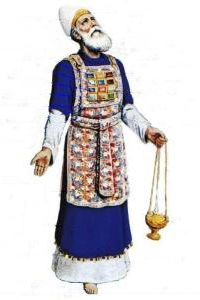
\includegraphics[width=50mm,scale=1.5]{Extras/Melchisedec.jpg}
\vspace{0.4in}  % Create a title for the document and write it in bold font
\LARGE{\textbf{\date}} % Again, do a line break
\linebreak 
% Create a subtitle \large{with Outlines, Statistics, Cross References, and Notes}
\vspace{0.5in}
\begin{flushleft}
\LARGE{Day \#67: Tuesday, 8 March 2022  \\}\vspace{0.25in}
\LARGE{Joshua 7-9 Psalm 67 Proverb 8}
\end{flushleft}
\vspace{0.6in}
\bigskip

\normalsize{Xenia, Oh.\\}
\normalsize{created: \today}
\vspace{1.3in}

\end{flushright}
\end{titlepage}

\newpage 
\tableofcontents\hypertarget{TOC}{}
\listoffigures
\listoftables

\hyphenation{A-bim-e-lech bre-thren E-phra-im  Gib-e-o-nites Jer-u-sa-lem through-out Phil-i-stines The-o-phil-us Am-a-le-kites ven-geance Mesh-el-e-mi-ah onan-ism Phar-a-oh thoughts grev-ous-ness Hach-a-liah adul-ter-er Shad-rach}

%%%%%%%%%%%%%%%%% EXTRA COLORS
%%%%%%%%%%%%%%%%% EXTRA COLORS
%%%%%%%%%%%%%%%%% EXTRA COLORS
\definecolor{champagne}{rgb}{0.97,0.91,0.81}
\definecolor{bone}{rgb}{0.89,0.85,0.79}

\definecolor{ForestGreen}{rgb}{0.00,0.29,0.098}
\definecolor{GIVING}{cmyk}{1,0.0,0.72,.1}

\definecolor{MLPE}{cmyk}{1,1,0,.45}
\definecolor{SOCCER}{cmyk}{.77, 0, .42, .49}
\definecolor{PAYBILL}{cmyk}{0,0.83,0.76,0.07}
\definecolor{SERMON}{cmyk}{.14,.9,0,.30} % aka seance \href{http://www.flatuicolorpicker.com/purple-cmyk-color-model/}{seance}
\definecolor{BIBLE}{cmyk}{0,.17,.74,.17}
\definecolor{WORKBLUE}{cmyk}{1, .5, 0, .6}
\definecolor{myOrange}{cmyk}{0, .4, .98, .03}
\definecolor{myTan}{cmyk}{0.0,.07,.17,.10}
\definecolor{myRed}{cmyk}{0,1,1,0}
\definecolor{myWhite}{cmyk}{0,0,0,0}
\definecolor{BLUESoD}{cmyk}{.97,.84,0,.04}
\definecolor{WHITE}{cmyk}{0,0,0,0}
\definecolor{OLDGOLD}{cmyk}{0.05,0.3,1.00,0}
\definecolor{CASTLETON}{cmyk}{1,0,0.31,0.66}
\definecolor{cadmiumgreen}{rgb}{0.0, 0.42, 0.24}
\definecolor{jungle}{rgb}{0.203,0.4882,0.1718}
\definecolor{MYGOLD}{rgb}{1,.84,0}

\definecolor{MYLIGHTGRAY}{rgb}{.85,.85,.85}

\definecolor{codegreen}{rgb}{0,0.6,0}
\definecolor{codegray}{rgb}{0.5,0.5,0.5}
\definecolor{codepurple}{rgb}{0.58,0,0.82}
\definecolor{backcolour}{rgb}{0.95,0.95,0.92}


\mdfdefinestyle{MyFrame}{%
    linecolor=blue,
    outerlinewidth=2pt,
    roundcorner=5pt,
    innertopmargin=\baselineskip,
    innerbottommargin=\baselineskip,
    innerrightmargin=10pt,
    innerleftmargin=10pt,
    backgroundcolor=gray!25!white}


\mdfdefinestyle{MyFrame2}{%
    linecolor=black,
    outerlinewidth=2pt,
    roundcorner=5pt,
    innertopmargin=\baselineskip,
    innerbottommargin=\baselineskip,
    innerrightmargin=10pt,
    innerleftmargin=10pt,
    backgroundcolor=yellow!25!white}


%%%%%
%% for PFTTIS list
%%%%%

%%% And Joseph said unto
\index[PFTTIS]{And Joseph said unto!Genesis!Gen 40:008}
\index[PFTTIS]{And Joseph said unto!Genesis!Gen 40:012}
\index[PFTTIS]{And Joseph said unto!Genesis!Gen 41:025}
\index[PFTTIS]{And Joseph said unto!Genesis!Gen 42:014}
\index[PFTTIS]{And Joseph said unto!Genesis!Gen 42:018}
\index[PFTTIS]{And Joseph said unto!Genesis!Gen 44:015}
\index[PFTTIS]{And Joseph said unto!Genesis!Gen 45:003}
\index[PFTTIS]{And Joseph said unto!Genesis!Gen 45:004}
\index[PFTTIS]{And Joseph said unto!Genesis!Gen 46:031}
\index[PFTTIS]{And Joseph said unto!Genesis!Gen 48:009}
\index[PFTTIS]{And Joseph said unto!Genesis!Gen 48:018}
\index[PFTTIS]{And Joseph said unto!Genesis!Gen 50:019}
\index[PFTTIS]{And Joseph said unto!Genesis!Gen 50:024}


%%% a shadow
\index[PFTTIS]{a shadow!1Chronicles!1Chr 029:15}
\index[PFTTIS]{a shadow!Job!Job 008:09}
\index[PFTTIS]{a shadow!Job!Job 014:02}
\index[PFTTIS]{a shadow!Job!Job 017:07}
\index[PFTTIS]{a shadow!Psalm!Psa 102:011}
\index[PFTTIS]{a shadow!Psalm!Psa 144:004}
\index[PFTTIS]{a shadow!Ecclesiastes!Eccl 006:012}
\index[PFTTIS]{a shadow!Ecclesiastes!Eccl 008:013}
\index[PFTTIS]{a shadow!Isaiah!Isa 04:006}
\index[PFTTIS]{a shadow!Isaiah!Isa 25:004}
\index[PFTTIS]{a shadow!Jonah!Jnh 04:06}
\index[PFTTIS]{a shadow!Colossians!Col 02:017}
\index[PFTTIS]{a shadow!Hebews!Heb 10:001}

%%% blessed is the man
\index[PFTTIS]{blessed is the man!Psalm!Psa 001:001}
\index[PFTTIS]{blessed is the man!Psalm!Psa 032:002}
\index[PFTTIS]{blessed is the man!Psalm!Psa 034:008}
\index[PFTTIS]{blessed is the man!Psalm!Psa 065:004}
\index[PFTTIS]{blessed is the man!Psalm!Psa 084:005}
\index[PFTTIS]{blessed is the man!Psalm!Psa 084:012}
\index[PFTTIS]{blessed is the man!Psalm!Psa 094:012}
\index[PFTTIS]{blessed is the man!Psalm!Psa 112:001}
\index[PFTTIS]{blessed is the man!Proverbs!Pro 008:034}
\index[PFTTIS]{blessed is the man!Isaiah!Isa 056:002}
\index[PFTTIS]{blessed is the man!Jeremiah!Jer 017:007}
\index[PFTTIS]{blessed is the man!Romans!Rom 004:008}
\index[PFTTIS]{blessed is the man!James!Jam 001:012}


%%% carry them
\index[PFTTIS]{carry them!Leviticus!Lev 14:045}
\index[PFTTIS]{carry them!Numbers!Num 11:012}
\index[PFTTIS]{carry them!Joshua!Jsh 04:003}
\index[PFTTIS]{carry them!1Samuel!1Sam 20:040}
\index[PFTTIS]{carry them!1Kings!1Kng 08:046}
\index[PFTTIS]{carry them!2Chronicles!2Chr 06:036}
\index[PFTTIS]{carry them!Ezra!Ezra 05:015}
\index[PFTTIS]{carry them!Isaiah!Isa 40:011}
\index[PFTTIS]{carry them!Isaiah!Isa 41:016}
\index[PFTTIS]{carry them!Isaiah!Isa 57:013}
\index[PFTTIS]{carry them!Jeremiah!Jer 20:004}
\index[PFTTIS]{carry them!Jeremiah!Jer 20:005}
\index[PFTTIS]{carry them!Jeremiah!Jer 43:012}


\index[PFTTIS]{good tidings!2Samuel!2Sam 18:027}
\index[PFTTIS]{good tidings!1Kings!1Ki 01:042}
\index[PFTTIS]{good tidings!2Kings!2Ki 07:009 (2x)}
\index[PFTTIS]{good tidings!Isaiah!Isa 40:009 (2x)}
\index[PFTTIS]{good tidings!Isaiah!Isa 41:007}
\index[PFTTIS]{good tidings!Isaiah!Isa 52:007}
\index[PFTTIS]{good tidings!Isaiah!Isa 61:001}
\index[PFTTIS]{good tidings!Nahum!Nah 01:005}
\index[PFTTIS]{good tidings!Luke!Lk 02:010}
\index[PFTTIS]{good tidings!1Thessalonians!1Thess 03:006}


%%% dead body
\index[PFTTIS]{dead body!Leviticus!Lev 21:011}
\index[PFTTIS]{dead body!Numbers!Num 06:006}
\index[PFTTIS]{dead body!Numbers!Num 09:006}
\index[PFTTIS]{dead body!Numbers!Num 09:007}
\index[PFTTIS]{dead body!Numbers!Num 09:010}
\index[PFTTIS]{dead body!Numbers!Num 09:011}
\index[PFTTIS]{dead body!Numbers!Num 09:013}
\index[PFTTIS]{dead body!Numbers!Num 09:016}
\index[PFTTIS]{dead body!2Kings!2Ki 08:005}
\index[PFTTIS]{dead body!Isaiah!Isa 26:019}
\index[PFTTIS]{dead body!Jeremiah!Jer 26:023}
\index[PFTTIS]{dead body!Jeremiah!Jer 36:030}
\index[PFTTIS]{dead body!Haggai!Hag 02:013}

%%% great sea
\index[PFTTIS]{great sea!Numbers!Num 34:006}
\index[PFTTIS]{great sea!Numbers!Num 34:007}
\index[PFTTIS]{great sea!Joshua!Jos 01:004}
\index[PFTTIS]{great sea!Joshua!Jos 09:001}
\index[PFTTIS]{great sea!Joshua!Jos 15:012}
\index[PFTTIS]{great sea!Joshua!Jos 15:047}
\index[PFTTIS]{great sea!Joshua!Jos 23:004}
\index[PFTTIS]{great sea!Ezekiel!Eze 47:010}
\index[PFTTIS]{great sea!Ezekiel!Eze 47:015}
\index[PFTTIS]{great sea!Ezekiel!Eze 47:019}
\index[PFTTIS]{great sea!Ezekiel!Eze 47:020}
\index[PFTTIS]{great sea!Ezekiel!Eze 48:028}
\index[PFTTIS]{great sea!Daniel!Dan 07:002}


%%% have forsaken me
\index[PFTTIS]{have forsaken me!Judges!Jdg 10:013}
\index[PFTTIS]{have forsaken me!1Samuel!1Sam 08:008}
\index[PFTTIS]{have forsaken me!1Kings!1Ki 11:033}
\index[PFTTIS]{have forsaken me!2Kings!2Ki 22:017}
\index[PFTTIS]{have forsaken me!2Chronicles!2Chr 12:005}
\index[PFTTIS]{have forsaken me!2Chronicles!2Chr 34:025}
\index[PFTTIS]{have forsaken me!Jeremiah!Jer 01:016}
\index[PFTTIS]{have forsaken me!Jeremiah!Jer 02:013}
\index[PFTTIS]{have forsaken me!Jeremiah!Jer 05:007}
\index[PFTTIS]{have forsaken me!Jeremiah!Jer 05:019}
\index[PFTTIS]{have forsaken me!Jeremiah!Jer 16:011 (2x)}
\index[PFTTIS]{have forsaken me!Jeremiah!Jer 19:004}

%%% no king
\index[PFTTIS]{no king!Judges!Jdg 17:06}
\index[PFTTIS]{no king!Judges!Jdg 18:01}
\index[PFTTIS]{no king!Judges!Jdg 19:01}
\index[PFTTIS]{no king!Judges!Jdg 21:25}
\index[PFTTIS]{no king!1Kings!1Ki 22:47}
\index[PFTTIS]{no king!2Kings!2Ki 23:25}
\index[PFTTIS]{no king!Nehemiah!Neh 13:26}
\index[PFTTIS]{no king!Psalms!Psa 033:016}
\index[PFTTIS]{no king!Proverbs!Pro 30:27}
\index[PFTTIS]{no king!Daniel!Dan 02:10}
\index[PFTTIS]{no king!Hosea!Hos 10:03}
\index[PFTTIS]{no king!Micah!Mic 04:09}
\index[PFTTIS]{no king!John!Jhn 19:15}


%%% rebellious house
\index[PFTTIS]{rebellious house!Exodus!Exo 02:005}
\index[PFTTIS]{rebellious house!Exodus!Exo 02:006}
\index[PFTTIS]{rebellious house!Exodus!Exo 02:008}
\index[PFTTIS]{rebellious house!Exodus!Exo 03:009}
\index[PFTTIS]{rebellious house!Exodus!Exo 03:026}
\index[PFTTIS]{rebellious house!Exodus!Exo 03:027}
\index[PFTTIS]{rebellious house!Exodus!Exo 12:002 (2x)}
\index[PFTTIS]{rebellious house!Exodus!Exo 12:003}
\index[PFTTIS]{rebellious house!Exodus!Exo 12:009}
\index[PFTTIS]{rebellious house!Exodus!Exo 12:025}
\index[PFTTIS]{rebellious house!Exodus!Exo 17:012}
\index[PFTTIS]{rebellious house!Exodus!Exo 24:003}

%%% seek him
\index[PFTTIS]{seek him!Deuteronomy!Deu 04:029}\index[PFTTIS]{seek him!1Samuel!1Sam 23:025}
\index[PFTTIS]{seek him!1Chronicles!1Chr 28:009}
\index[PFTTIS]{seek him!2Chronicles!1Chr 15:002}
\index[PFTTIS]{seek him!Ezra!Ezr 08:022}
\index[PFTTIS]{seek him!Psalms!Psa 022:026}
\index[PFTTIS]{seek him!Psalms!Psa 024:006}
\index[PFTTIS]{seek him!Psalms!Psa 119:002}
\index[PFTTIS]{seek him!SoS!SoS 03:002}
\index[PFTTIS]{seek him!SoS!SoS 06:001}
\index[PFTTIS]{seek him!Hosea!Hos 07:010}
\index[PFTTIS]{seek him!Amos!Amo 05:008}
\index[PFTTIS]{seek him!Hebrews!Heb 11:0063}


%%% seek ye
\index[PFTTIS]{seek ye!Isaiah!Isa 34:016}
\index[PFTTIS]{seek ye!Isaiah!Isa 45:019}
\index[PFTTIS]{seek ye!Isaiah!Isa 55:006}
\index[PFTTIS]{seek ye!Amos!Amos 5:004}
\index[PFTTIS]{seek ye!John!John 1:38}
\index[PFTTIS]{seek ye!John!John 18:4}
\index[PFTTIS]{seek ye!John!John 18:7}
\index[PFTTIS]{seek ye!Matthew!Matt 6:33}
\index[PFTTIS]{seek ye!Numbers!Num 16:10}
\index[PFTTIS]{seek ye!Luke!Luke 12:31}
\index[PFTTIS]{seek ye!Luke!Luke 24:5}
\index[PFTTIS]{seek ye!Psalm!Psa 27:8}
\index[PFTTIS]{seek ye!Zephaniah!Zeph 2:3}

%%% the uncircumcised
\index[PFTTIS]{the uncircumcised!Genesis!Gen 17:014}
\index[PFTTIS]{the uncircumcised!Judges!Jdg 14:003}
\index[PFTTIS]{the uncircumcised!Judges!Jdg 15:018}
\index[PFTTIS]{the uncircumcised!2Samuel!2Sam 01:020}
\index[PFTTIS]{the uncircumcised!Isaiah!Isa 02:001}
\index[PFTTIS]{the uncircumcised!Jeremiah!Jer 09:025}
\index[PFTTIS]{the uncircumcised!Ezekiel!Eze 28:010}
\index[PFTTIS]{the uncircumcised!Ezekiel!Eze 31:018}
\index[PFTTIS]{the uncircumcised!Ezekiel!Eze 32:019}
\index[PFTTIS]{the uncircumcised!Ezekiel!Eze 32:027}
\index[PFTTIS]{the uncircumcised!Ezekiel!Eze 32:028}
\index[PFTTIS]{the uncircumcised!Ezekiel!Eze 32:029}
\index[PFTTIS]{the uncircumcised!Ezekiel!Eze 32:032}

%%% worship him
\index[PFTTIS]{worship him!Psalms!Psa 97:007}
\index[PFTTIS]{worship him!Zephaniah!Zeph 02:011}
\index[PFTTIS]{worship him!Matthew!Matt 02:002}
\index[PFTTIS]{worship him!Matthew!Matt 02:008}
\index[PFTTIS]{worship him!John!John 04:023}
\index[PFTTIS]{worship him!John!John 04:024 (2x)} 
\index[PFTTIS]{worship him!Acts!Acts 17:023}
\index[PFTTIS]{worship him!Hebrews!Heb 01:006}
\index[PFTTIS]{worship him!Revelation!Rev 04:010}
\index[PFTTIS]{worship him!Revelation!Rev 13:008}
\index[PFTTIS]{worship him!Revelation!Rev 14:007}
\index[PFTTIS]{worship him!Revelation!Rev 19:010}


%%%%%
%% for PFTTIS list
%%%%%

%%% afflictions
\index[WFTTIS]{afflictions!Psalms!Psa 34:019}
\index[WFTTIS]{afflictions!Psalms!Psa 132:001}
\index[WFTTIS]{afflictions!Acts!Acts 07:010}
\index[WFTTIS]{afflictions!Acts!Acts 20:023}
\index[WFTTIS]{afflictions!2Corinthians!2Cor 06:004}
\index[WFTTIS]{afflictions!Colossians!Col 01:024}
\index[WFTTIS]{afflictions!1Thessalonians!1Thess 03:003}
\index[WFTTIS]{afflictions!2Timothy!2Tim 01:008}
\index[WFTTIS]{afflictions!2Timothy!2Tim 03:011}
\index[WFTTIS]{afflictions!2Timothy!2Tim 04:005}
\index[WFTTIS]{afflictions!Hebrews!Heb 10:032}
\index[WFTTIS]{afflictions!Hebrews!Heb 10:033}
\index[WFTTIS]{afflictions!1Peter!1Pet 05:009}

%%% acsend
\index[WFTTIS]{acsend!Joshua!Jos 06:05}
\index[WFTTIS]{acsend!Psalm!Psa 024:003}
\index[WFTTIS]{acsend!Psalm!Psa 135:007}
\index[WFTTIS]{acsend!Psalm!Psa 139:008}
\index[WFTTIS]{acsend!Isaiah!Isa 14:013}
\index[WFTTIS]{acsend!Isaiah!Isa 14:014}
\index[WFTTIS]{acsend!Jeremiah!Jer 10:013}
\index[WFTTIS]{acsend!Jeremiah!Jer 51:016}
\index[WFTTIS]{acsend!Ezekiel!Eze 38:009}
\index[WFTTIS]{acsend!John!John 06:062}
\index[WFTTIS]{acsend!John!John 20:017}
\index[WFTTIS]{acsend!Romans!Rom 10:006}
\index[WFTTIS]{acsend!Revelation!Rev 17:008}

%%% Assyrian
\index[WFTTIS]{Assyrian!Isaiah!Isa 10:005}
\index[WFTTIS]{Assyrian!Isaiah!Isa 10:024}
\index[WFTTIS]{Assyrian!Isaiah!Isa 14:025}
\index[WFTTIS]{Assyrian!Isaiah!Isa 19:023}
\index[WFTTIS]{Assyrian!Isaiah!Isa 23:013}
\index[WFTTIS]{Assyrian!Isaiah!Isa 30:031}
\index[WFTTIS]{Assyrian!Isaiah!Isa 31:008}
\index[WFTTIS]{Assyrian!Isaiah!Isa 52:004}
\index[WFTTIS]{Assyrian!Ezekiel!Eze 31:003}
\index[WFTTIS]{Assyrian!Hosea!Hos 05:013}
\index[WFTTIS]{Assyrian!Hosea!Hos 11:005}
\index[WFTTIS]{Assyrian!Micah!Hos 05:005}
\index[WFTTIS]{Assyrian!Micah!Hos 05:006}

%%% blot
\index[WFTTIS]{blot!Exodus!Exo 32:032}
\index[WFTTIS]{blot!Exodus!Exo 32:033}
\index[WFTTIS]{blot!Numbers!Num 05:026}
\index[WFTTIS]{blot!Deuteronomy!Deut 09:014}
\index[WFTTIS]{blot!Deuteronomy!Deut 25:019}
\index[WFTTIS]{blot!Deuteronomy!Deut 29:020}
\index[WFTTIS]{blot!2Kings!2Ki 14:027}
\index[WFTTIS]{blot!Job!Job 31:007}
\index[WFTTIS]{blot!Psalms!Psa 51:001}
\index[WFTTIS]{blot!Psalms!Psa 51:009}
\index[WFTTIS]{blot!Proverbs!Pro 09:007}
\index[WFTTIS]{blot!Jeremiah!Jer 18:023}
\index[WFTTIS]{blot!Revelation!Rev 03:005}


%%% chain
\index[WFTTIS]{chain!Genesis!Gen 41:042}
\index[WFTTIS]{chain!1Kings!1Ki 07:017}
\index[WFTTIS]{chain!Psalms!Psa 73:006}
\index[WFTTIS]{chain!SoS!Sos 04:009}
\index[WFTTIS]{chain!Lamentations!Lam 03:007}
\index[WFTTIS]{chain!Ezekiel!Eze 07:023}
\index[WFTTIS]{chain!Ezekiel!Eze 16:011}
\index[WFTTIS]{chain!Daniel!Dan 05:007}
\index[WFTTIS]{chain!Daniel!Dan 05:016}
\index[WFTTIS]{chain!Daniel!Dan 05:029}
\index[WFTTIS]{chain!Acts!Acts 28:020}
\index[WFTTIS]{chain!2Timothy!2Tim 01:016}
\index[WFTTIS]{chain!Revelation!Rev 20:001}


%%% controversy
\index[WFTTIS]{controversy!Deuteronomy!Deu 17:008}
\index[WFTTIS]{controversy!Deuteronomy!Deu 19:017}
\index[WFTTIS]{controversy!Deuteronomy!Deu 21:005}
\index[WFTTIS]{controversy!Deuteronomy!Deu 25:001}
\index[WFTTIS]{controversy!2Samuel!2Sam 15:002}
\index[WFTTIS]{controversy!Isaiah!Isa 34:008}
\index[WFTTIS]{controversy!Jeremiah!Jer 25:031}
\index[WFTTIS]{controversy!Ezekiel!Eze 44:024}
\index[WFTTIS]{controversy!Hosea!Hos 04:001}
\index[WFTTIS]{controversy!Hosea!Hos 12:002}
\index[WFTTIS]{controversy!Micah!Mic 06:002 (2x)}
\index[WFTTIS]{controversy!1Timothy!1Tim 03:016}


%%% Dagon/Dagon's
\index[WFTTIS]{Dagon!Judges!Jdg 16:023}
\index[WFTTIS]{Dagon!1Samuel!1Sam 05:002 (2x)}
\index[WFTTIS]{Dagon!1Samuel!1Sam 05:003 (2x)}
\index[WFTTIS]{Dagon!1Samuel!1Sam 05:004 (3x)}
\index[WFTTIS]{Dagon!1Samuel!1Sam 05:005 (3x)}
\index[WFTTIS]{Dagon!1Samuel!1Sam 05:007}
\index[WFTTIS]{Dagon!1Chronicles!1Chr 10:010}

%%% disobedient
\index[WFTTIS]{disobedient!1Kings!1Ki 13:026}
\index[WFTTIS]{disobedient!Nehemiah!Neh 09:026}
\index[WFTTIS]{disobedient!Luke!Luke 01:017}
\index[WFTTIS]{disobedient!Acts!Acts 26:019}
\index[WFTTIS]{disobedient!Romans!Rom 01:030}
\index[WFTTIS]{disobedient!Romans!Rom 10:021}
\index[WFTTIS]{disobedient!1Timothy!1Tim 01:009}
\index[WFTTIS]{disobedient!2Timothy!2Tim 03:002}
\index[WFTTIS]{disobedient!Titus!Titus 01:016}
\index[WFTTIS]{disobedient!Titus!Titus 03:003}
\index[WFTTIS]{disobedient!1Peter!1Pet 02:007}
\index[WFTTIS]{disobedient!1Peter!1Pet 02:008}
\index[WFTTIS]{disobedient!1Peter!1Pet 03:020}


%%% doubt
\index[WFTTIS]{doubt!Genesis!Gen 37:033}
\index[WFTTIS]{doubt!Deuteronomy!Deu 28:066}
\index[WFTTIS]{doubt!Job!Job 12:002}
\index[WFTTIS]{doubt!Matthew!Matt 14:031}
\index[WFTTIS]{doubt!Matthew!Matt 21:021}
\index[WFTTIS]{doubt!Mark!Mk 11:023}
\index[WFTTIS]{doubt!Luke!Lk 11:020}
\index[WFTTIS]{doubt!John!Jhn 10:024}
\index[WFTTIS]{doubt!Acts!Acts 02:012}
\index[WFTTIS]{doubt!Acts!Acts 28:004}
\index[WFTTIS]{doubt!1Corinthians!1Cor 09:010}
\index[WFTTIS]{doubt!Galatians!Gal 04:020}
\index[WFTTIS]{doubt!1John!1Jhn 02:019}


%%% dungeon
\index[WFTTIS]{dungeon!Genesis!Gen 40:015}
\index[WFTTIS]{dungeon!Genesis!Gen 41:014}
\index[WFTTIS]{dungeon!Exodus!Exo 12:029}
\index[WFTTIS]{dungeon!Jeremiah!Jer 37:016}
\index[WFTTIS]{dungeon!Jeremiah!Jer 38:006 (2x)}
\index[WFTTIS]{dungeon!Jeremiah!Jer 38:007}
\index[WFTTIS]{dungeon!Jeremiah!Jer 38:009}
\index[WFTTIS]{dungeon!Jeremiah!Jer 38:010}
\index[WFTTIS]{dungeon!Jeremiah!Jer 38:011}
\index[WFTTIS]{dungeon!Jeremiah!Jer 38:013}
\index[WFTTIS]{dungeon!Lamentations!Lam 03:053}
\index[WFTTIS]{dungeon!Lamentations!Lam 03:055}


%%% error
\index[WFTTIS]{error!2Samuel!2Sam 06:007}
\index[WFTTIS]{error!Job!Job 19:004}
\index[WFTTIS]{error!Ecclesiastes!Ecc 05:006}
\index[WFTTIS]{error!Ecclesiastes!Ecc 10:005}
\index[WFTTIS]{error!Isaiah!Isa 32:006}
\index[WFTTIS]{error!Daniel!Dan 06:004}
\index[WFTTIS]{error!Matthew!Matt 27:064}
\index[WFTTIS]{error!Romans!Rom 01:027}
\index[WFTTIS]{error!James!Jam 05:020}
\index[WFTTIS]{error!2Peter!2Pet 02:018}
\index[WFTTIS]{error!2Peter!2Pet 03:017}
\index[WFTTIS]{error!1John!1Jn 04:006}
\index[WFTTIS]{error!Jude!Jude 01:011}

%%% fourish
\index[WFTTIS]{fourish!Psalms!Psa 072:007}
\index[WFTTIS]{fourish!Psalms!Psa 072:016}
\index[WFTTIS]{fourish!Psalms!Psa 092:007}
\index[WFTTIS]{fourish!Psalms!Psa 092:012}
\index[WFTTIS]{fourish!Psalms!Psa 092:013}
\index[WFTTIS]{fourish!Psalms!Psa 132:018}
\index[WFTTIS]{fourish!Proverbs!Pro 11:28}
\index[WFTTIS]{fourish!Proverbs!Pro 14:11}
\index[WFTTIS]{fourish!Ecclesiastes!Ecc 12:05}
\index[WFTTIS]{fourish!SongOfSolomon!SOS 07:12}
\index[WFTTIS]{fourish!Isaiah!Isa 17:11}
\index[WFTTIS]{fourish!Isaiah!Isa 66:14}
\index[WFTTIS]{fourish!Ezekiel!Eze 17:24}




%%% giants
\index[WFTTIS]{giants!Genesis!Gen 06:004}
\index[WFTTIS]{giants!Numbers!Num 13:033}
\index[WFTTIS]{giants!Deuteronomy!Deut 02:011}
\index[WFTTIS]{giants!Deuteronomy!Deut 02:021}
\index[WFTTIS]{giants!Deuteronomy!Deut 03:011}
\index[WFTTIS]{giants!Deuteronomy!Deut 03:013}
\index[WFTTIS]{giants!Joshua!Josh 12:004}
\index[WFTTIS]{giants!Joshua!Josh 13:012}
\index[WFTTIS]{giants!Joshua!Josh 15:008}
\index[WFTTIS]{giants!Joshua!Josh 17:015}
\index[WFTTIS]{giants!Joshua!Josh 16:016}

%%% good man
\index[WFTTIS]{good man!2 Samuel!2Sa 18:27}
%(1) Psalms 37:23 [5]
%(1) Psalms 112:5 [2]
%(1) Proverbs 12:2 [2]
%(1) Proverbs 13:22 [2]
%(1) Proverbs 14:14 [14]
%(1) Micah 7:2 [2]
%(1) Matthew 12:35 [2]
%(1) Luke 6:45 [2]
%(1) Luke 23:50 [15]
%(1) John 7:12 [17]
%(1) Acts 11:24 [5]
%(1) Romans 5:7 [14]

%%% Hinnom
\index[WFTTIS]{Hinnom!Joshua!Jsh 15:008}
\index[WFTTIS]{Hinnom!Joshua!Jsh 18:016}
\index[WFTTIS]{Hinnom!2Kings!2Ki 23:010}
\index[WFTTIS]{Hinnom!2Chronicles!2Chr 28:003}
\index[WFTTIS]{Hinnom!2Chronicles!2Chr 33:006}
\index[WFTTIS]{Hinnom!Nehemiah!Neh 11:030}
\index[WFTTIS]{Hinnom!Jeremiah!Jer 07:031}
\index[WFTTIS]{Hinnom!Jeremiah!Jer 07:032}
\index[WFTTIS]{Hinnom!Jeremiah!Jer 19:002}
\index[WFTTIS]{Hinnom!Jeremiah!Jer 19:006}
\index[WFTTIS]{Hinnom!Jeremiah!Jer 32:035}

%%% inclined
\index[WFTTIS]{inclined!Judges!Jdg 09:003}
\index[WFTTIS]{inclined!Psalms!Psa 040:001}
\index[WFTTIS]{inclined!Psalms!Psa 116:002}
\index[WFTTIS]{inclined!Psalms!Psa 119:112}
\index[WFTTIS]{inclined!Proverbs!Pro 05:13}
\index[WFTTIS]{inclined!Jeremiah!Jer 07:24}
\index[WFTTIS]{inclined!Jeremiah!Jer 07:26}
\index[WFTTIS]{inclined!Jeremiah!Jer 11:08}
\index[WFTTIS]{inclined!Jeremiah!Jer 17:23}
\index[WFTTIS]{inclined!Jeremiah!Jer 25:04}
\index[WFTTIS]{inclined!Jeremiah!Jer 34:14}
\index[WFTTIS]{inclined!Jeremiah!Jer 35:15}
\index[WFTTIS]{inclined!Jeremiah!Jer 44:05}


%%% laughed
\index[WFTTIS]{laughed!Genesis!Gen 17:017}
\index[WFTTIS]{laughed!Genesis!Gen 18:012}
\index[WFTTIS]{laughed!Genesis!Gen 18:015}
\index[WFTTIS]{laughed!2Kings!2Ki 19:021}
\index[WFTTIS]{laughed!2Chronicles!2Chr 30:010}
\index[WFTTIS]{laughed!Nehemiah!Neh 02:019}
\index[WFTTIS]{laughed!Job!Job 12:004}
\index[WFTTIS]{laughed!Job!Job 29:024}
\index[WFTTIS]{laughed!Isaiah!Isa 37:022}
\index[WFTTIS]{laughed!Ezekiel!Ezek 23:032}
\index[WFTTIS]{laughed!Matthew!Matt 09:024}
\index[WFTTIS]{laughed!Mark!Mk 05:040}
\index[WFTTIS]{laughed!Luke!Lk 08:053}

%%% liar
\index[WFTTIS]{liar!Job!Job 24:025}
\index[WFTTIS]{liar!Proverbs!Pro 17:004}
\index[WFTTIS]{liar!Proverbs!Pro 19:022}
\index[WFTTIS]{liar!Proverbs!Pro 30:006}
\index[WFTTIS]{liar!Jeremiah!Jer 15:018}
\index[WFTTIS]{liar!John!Jhn 08:044}
\index[WFTTIS]{liar!John!Jhn 08:055}
\index[WFTTIS]{liar!Romans!Rom 03:004}
\index[WFTTIS]{liar!1John!1Jhn 01:010}
\index[WFTTIS]{liar!1John!1Jhn 02:004}
\index[WFTTIS]{liar!1John!1Jhn 02:022}
\index[WFTTIS]{liar!1John!1Jhn 04:020}
\index[WFTTIS]{liar!1John!1Jhn 05:010}

%%% palsy
\index[WFTTIS]{palsy!Matthew!Matt 04:024}
\index[WFTTIS]{palsy!Matthew!Matt 08:006}
\index[WFTTIS]{palsy!Matthew!Matt 09:002}
\index[WFTTIS]{palsy!Matthew!Matt 09:006}
\index[WFTTIS]{palsy!Mark!Mk 02:003}
\index[WFTTIS]{palsy!Mark!Mk 02:004}
\index[WFTTIS]{palsy!Mark!Mk 02:005}
\index[WFTTIS]{palsy!Mark!Mk 02:009}
\index[WFTTIS]{palsy!Mark!Mk 02:010}
\index[WFTTIS]{palsy!Luke!Lk 05:018}
\index[WFTTIS]{palsy!Luke!Lk 05:024}
\index[WFTTIS]{palsy!Acts!Acts 09:033}

%%% Profitable
\index[WFTTIS]{profitable!Job!Job 22:002 (2x)}
\index[WFTTIS]{profitable!Ecclesiastes!Ecc 10:010}
\index[WFTTIS]{profitable!Isaiah!Isa 44:010}
\index[WFTTIS]{profitable!Jeremiah!Jer 13:007}
\index[WFTTIS]{profitable!Matthew!Matt 05:029}
\index[WFTTIS]{profitable!Matthew!Matt 05:030}
\index[WFTTIS]{profitable!Acts!Acts 20:020}
\index[WFTTIS]{profitable!1Timothy!1Tim 04:008}
\index[WFTTIS]{profitable!2Timothy!2Tim 03:016}
\index[WFTTIS]{profitable!2Timothy!2Tim 04:011}
\index[WFTTIS]{profitable!Titus!Titus 03:008}
\index[WFTTIS]{profitable!Philemon!Phlm 01:011}

%%% Rechab
\index[WFTTIS]{Rechab!2Samuel!2Sam 04:002}
\index[WFTTIS]{Rechab!2Samuel!2Sam 04:005}
\index[WFTTIS]{Rechab!2Samuel!2Sam 04:006}
\index[WFTTIS]{Rechab!2Samuel!2Sam 04:009}
\index[WFTTIS]{Rechab!2KIngs!2Ki 10:015}
\index[WFTTIS]{Rechab!2KIngs!2Ki 10:023}
\index[WFTTIS]{Rechab!1Chronicles!1Chr 02:055}
\index[WFTTIS]{Rechab!Nehemiah!Neh 03:014}
\index[WFTTIS]{Rechab!Jeremiah!Jer 35:006}
\index[WFTTIS]{Rechab!Jeremiah!Jer 35:008}
\index[WFTTIS]{Rechab!Jeremiah!Jer 35:014}
\index[WFTTIS]{Rechab!Jeremiah!Jer 35:016}
\index[WFTTIS]{Rechab!Jeremiah!Jer 35:019}

%%% serpents
\index[WFTTIS]{serpents!Exodus!Exo 07:012}
\index[WFTTIS]{serpents!Numbers!Num 21:006}
\index[WFTTIS]{serpents!Numbers!Num 21:007}
\index[WFTTIS]{serpents!Deuteronomy!Deu 08:015}
\index[WFTTIS]{serpents!Deuteronomy!Deu 32:024}
\index[WFTTIS]{serpents!Jeremiah!Jer 08:017}
\index[WFTTIS]{serpents!Matthew!Matt 10:016}
\index[WFTTIS]{serpents!Matthew!Matt 23:033}
\index[WFTTIS]{serpents!Mark!Mk 16:018}
\index[WFTTIS]{serpents!Luke!Lk 10:019}
\index[WFTTIS]{serpents!1Corinthians!1Cor 10:009}
\index[WFTTIS]{serpents!James!Jas 03:007}
\index[WFTTIS]{serpents!Revelation!Rev 09:019}

%%% short
\index[WFTTIS]{short!Numbers!Num 11:023}
\index[WFTTIS]{short!2Kings!2Ki 10:032}
\index[WFTTIS]{short!Job!Job 17:012}
\index[WFTTIS]{short!Job!Job 20:005}
\index[WFTTIS]{short!Psalms!Psa 89:047}
\index[WFTTIS]{short!Romans!Rom 03:023}
\index[WFTTIS]{short!Romans!Rom 09:028  (2x)}
\index[WFTTIS]{short!1Corinthians!1Cor 07:029}
\index[WFTTIS]{short!1Thessalonians!1Thess 02:017}
\index[WFTTIS]{short!Hebrews!Heb 04:001}
\index[WFTTIS]{short!Revelation!Rev 12:012}
\index[WFTTIS]{short!Revelation!Rev 17:010}

%%% smiteth
\index[WFTTIS]{smiteth!Exodus!Exo 21:012}
\index[WFTTIS]{smiteth!Exodus!Exo 21:15}
\index[WFTTIS]{smiteth!Deuteronomy!Dt 25:11}
\index[WFTTIS]{smiteth!Deuteronomy!Dt 27:24}
\index[WFTTIS]{smiteth!Joshua!Jsh 15:16}
\index[WFTTIS]{smiteth!Judges!Jdg 15:16}
\index[WFTTIS]{smiteth!2 Samuel!2Sa 05:08}
\index[WFTTIS]{smiteth!1Chronicles!1Chr 11:06}
\index[WFTTIS]{smiteth!Job!1Chr 26:12}
\index[WFTTIS]{smiteth!Isaiah!Isa 09:13}
\index[WFTTIS]{smiteth!Lamentations!Lam 03:30}
\index[WFTTIS]{smiteth!Ezekiel!Eze 07:09}
\index[WFTTIS]{smiteth!Luke!Lk 06:29}



%%% vanities
\index[WFTTIS]{vanities!Deuteronomy!Deut 21:021}
\index[WFTTIS]{vanities!1Kings!1Ki 16:013}
\index[WFTTIS]{vanities!1Kings!1Ki 16:026}
\index[WFTTIS]{vanities!Psalms!Psa 031:006}
\index[WFTTIS]{vanities!Ecclesiastes!Ecc 01:002 (2x)}
\index[WFTTIS]{vanities!Ecclesiastes!Ecc 05:007}
\index[WFTTIS]{vanities!Ecclesiastes!Ecc 12:008}
\index[WFTTIS]{vanities!Jeremiah!Jer 08:019}
\index[WFTTIS]{vanities!Jeremiah!Jer 10:008}
\index[WFTTIS]{vanities!Jeremiah!Jer 14:022}
\index[WFTTIS]{vanities!Jonah!Jnh 02:008}
\index[WFTTIS]{vanities!Acts!Acts 14:015}



%%%%%
%% for PFTTIS list
%%%%%

%%% worm
\index[WFITV]{worm!Exodus!Exo 16:024}
\index[WFITV]{worm!Job!Job 17:014}
\index[WFITV]{worm!Job!Job 24:029}
\index[WFITV]{worm!Job!Job 25:005 (2x)}
\index[WFITV]{worm!Psalms!Psa 022:006}
\index[WFITV]{worm!Isaiah!Isa 14:011}
\index[WFITV]{worm!Isaiah!Isa 41:014}
\index[WFITV]{worm!Isaiah!Isa 51:008}
\index[WFITV]{worm!Isaiah!Isa 66:024}
\index[WFITV]{worm!Jonah!Jnh 04:007}
\index[WFITV]{worm!Mark!Mk 09:044}
\index[WFITV]{worm!Mark!Mk 09:046}
\index[WFITV]{worm!Mark!Mk 09:048}


%\subsubsection{Title}
%\textbf{Introduction:} Isaiah 46 
%\index[speaker]{Speaker!Isaiah 49 (Title}
%\index[series]{Book (Speaker)!IPassage (Title)}
%\index[date]{2017/07/09!Isaiah 49 (Title)}
%\begin{compactenum}[I.]
%    \item  \textbf{Point} \index[scripture]{Isaiah!IPassage} (IPassage)
%\end{compactenum}




  


%\input{02OT-Exodus/ExodusIntroduction}

%\newpage
%\begin{figure}
%\begin{center}
%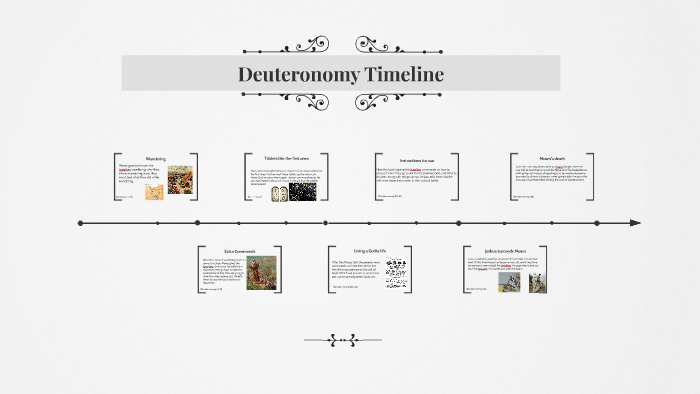
\includegraphics[scale=.7, angle=0]{05OT-Deuteronomy/References/AndrewSmithDeuteronomyTimeline.png}
%\caption[Deuteronomy Timeline by Andrew Smith]{Deuteronomy Timeline by Andrew %Smith}
%\label{fig:Deuteronomy Timeline by Andrew Smith}
%\end{center}
%\end{figure}

\newpage
\begin{figure}
\begin{center}
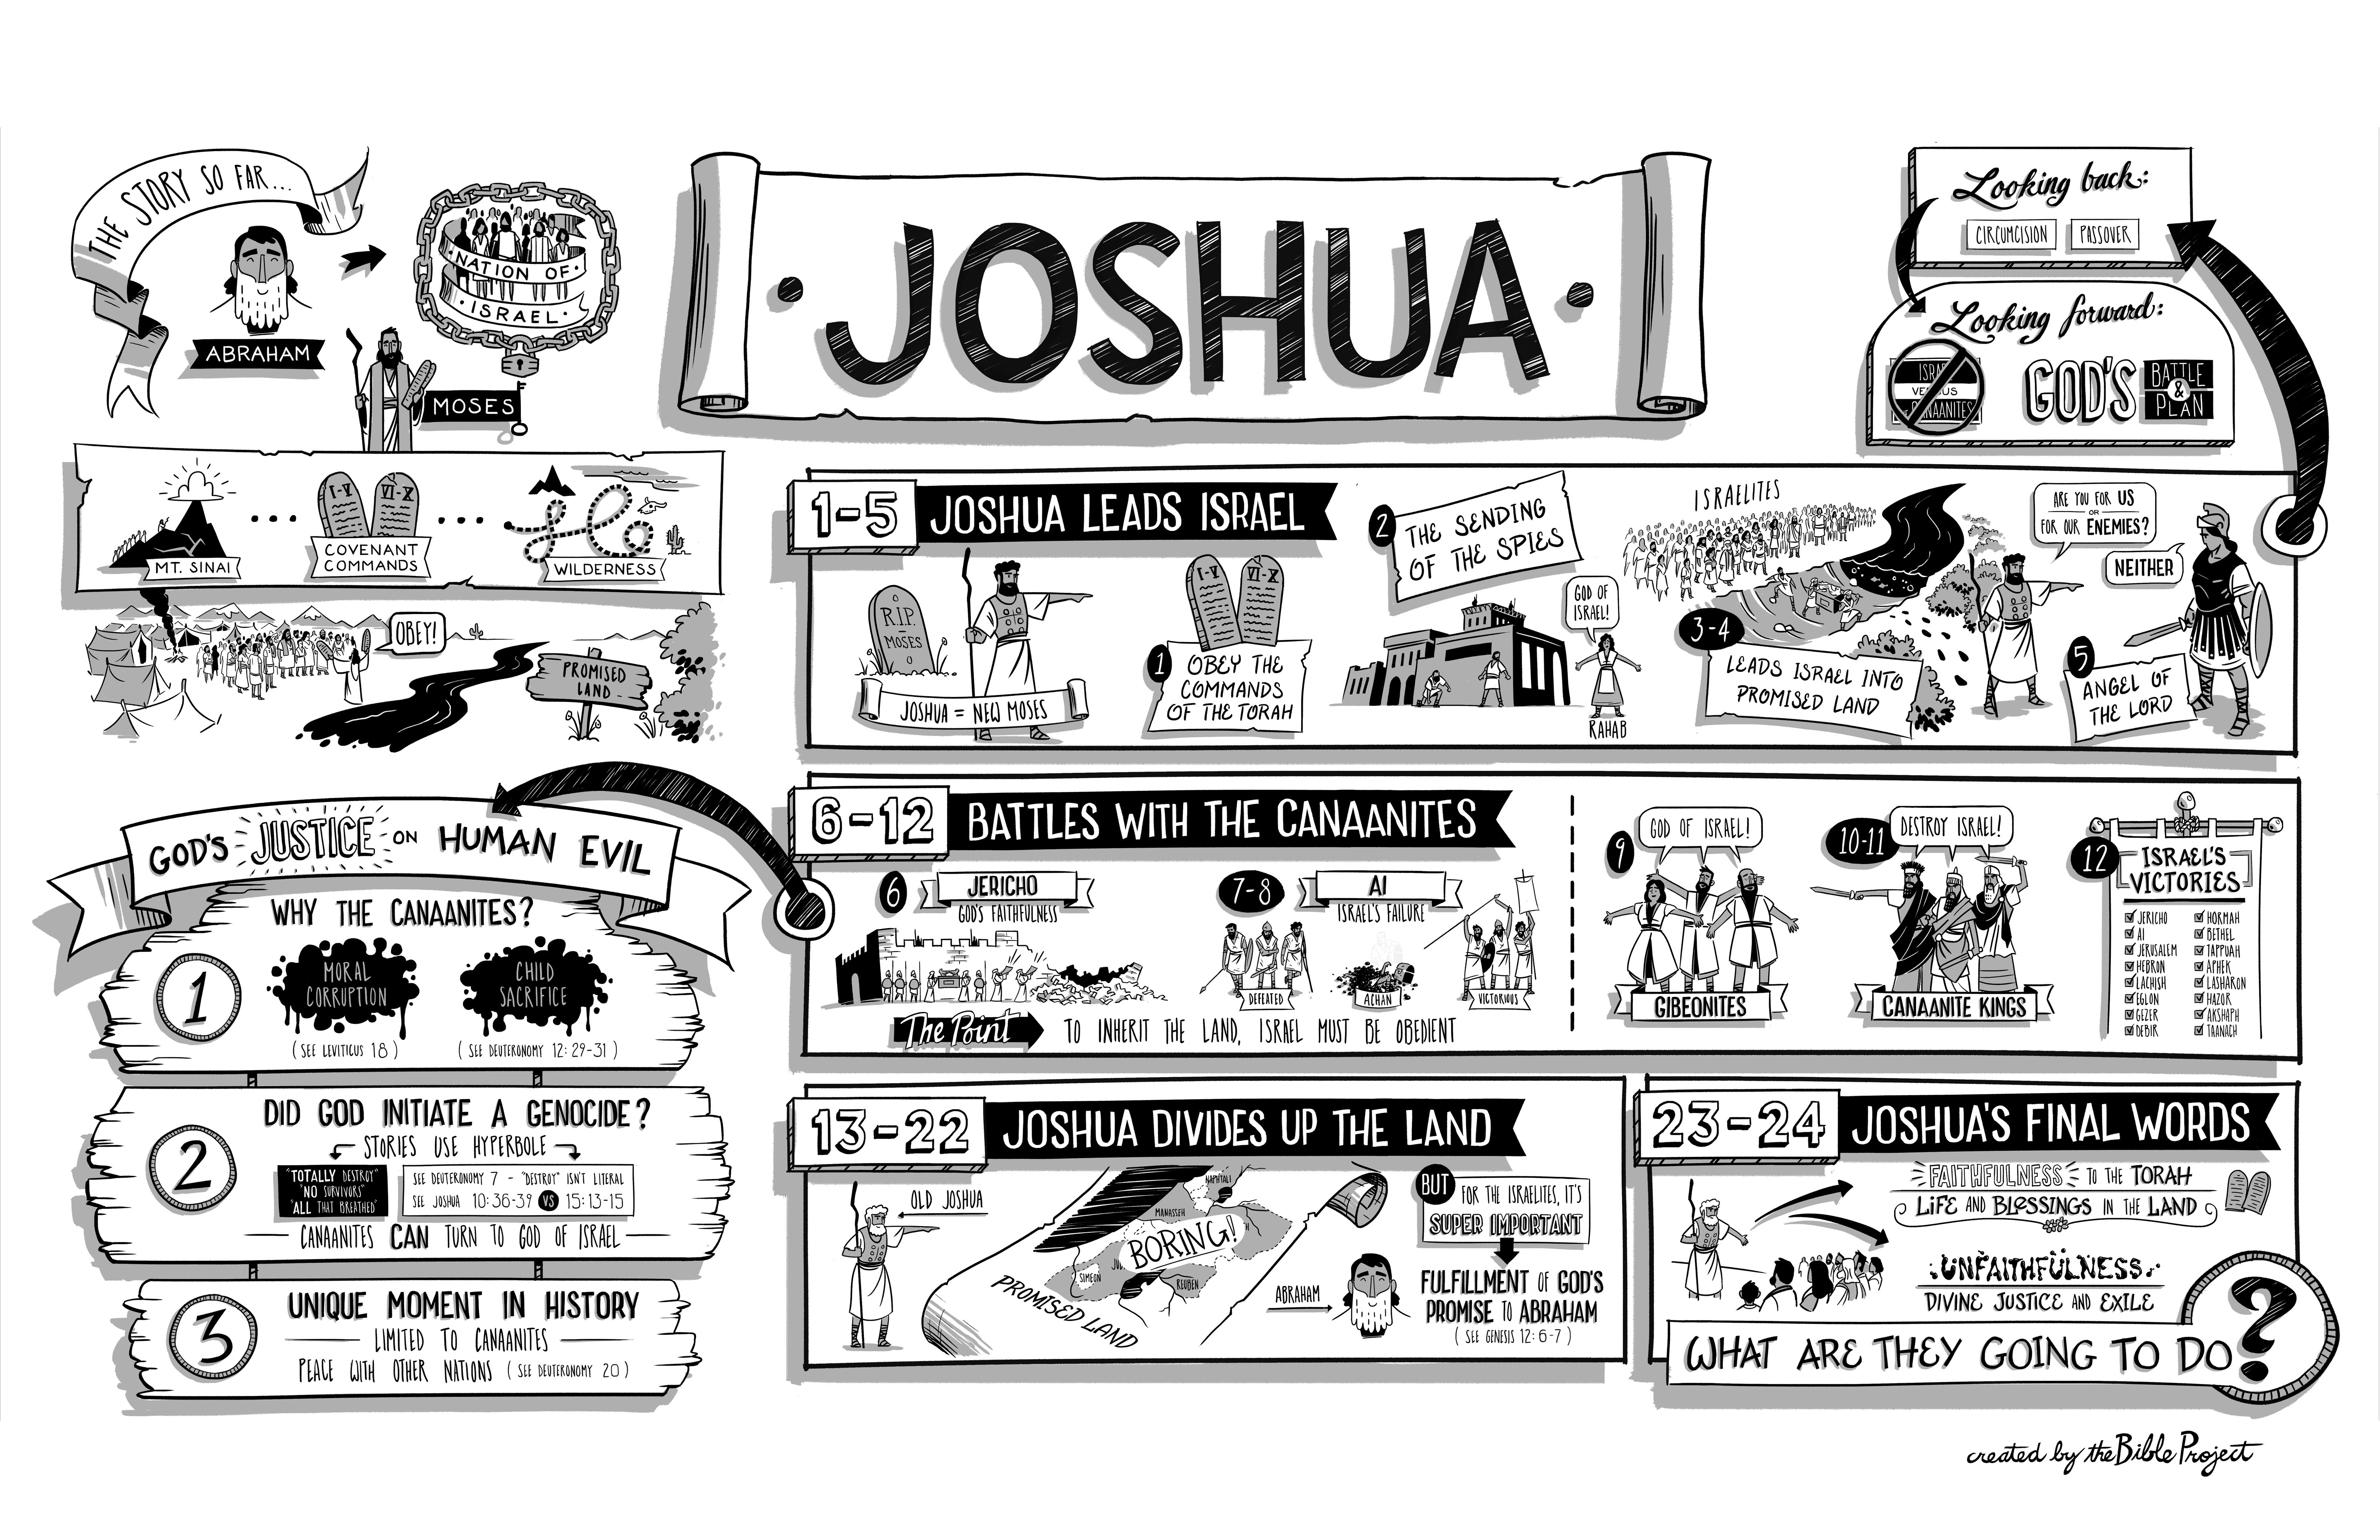
\includegraphics[scale=0.5, angle=90]{06OT-Joshua/References/1.BibleProject-Joshua.jpg}
\caption[Joshua from the Bible Project]{Joshua from the Bible Project}
\label{fig:Joshua from the Bible Project}
\end{center}
\end{figure}

\newpage
\begin{figure}
\begin{center}
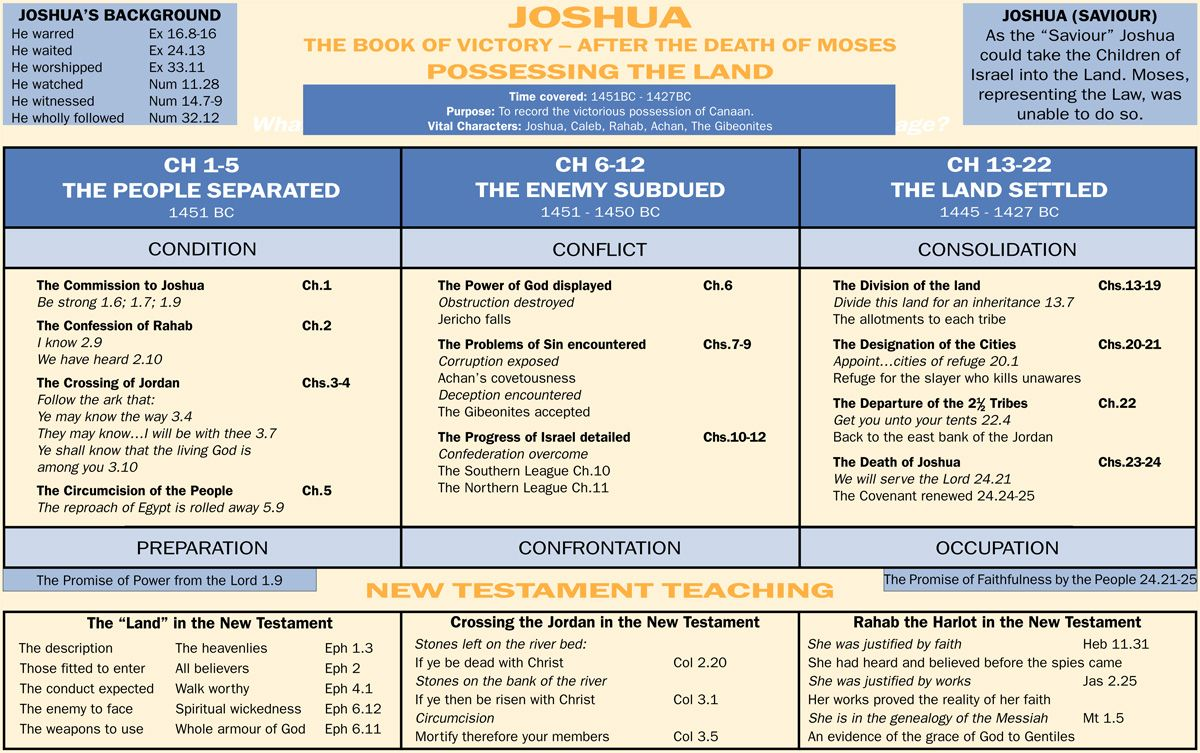
\includegraphics[scale=0.5, angle=90]{06OT-Joshua/References/2.JohnGrant-Joshua.jpg}
\caption[Joshua from John Grant]{Joshua from John Grant}
\label{fig:Joshua from John Grant}
\end{center}
\end{figure}

\newpage
\begin{figure}
\begin{center}
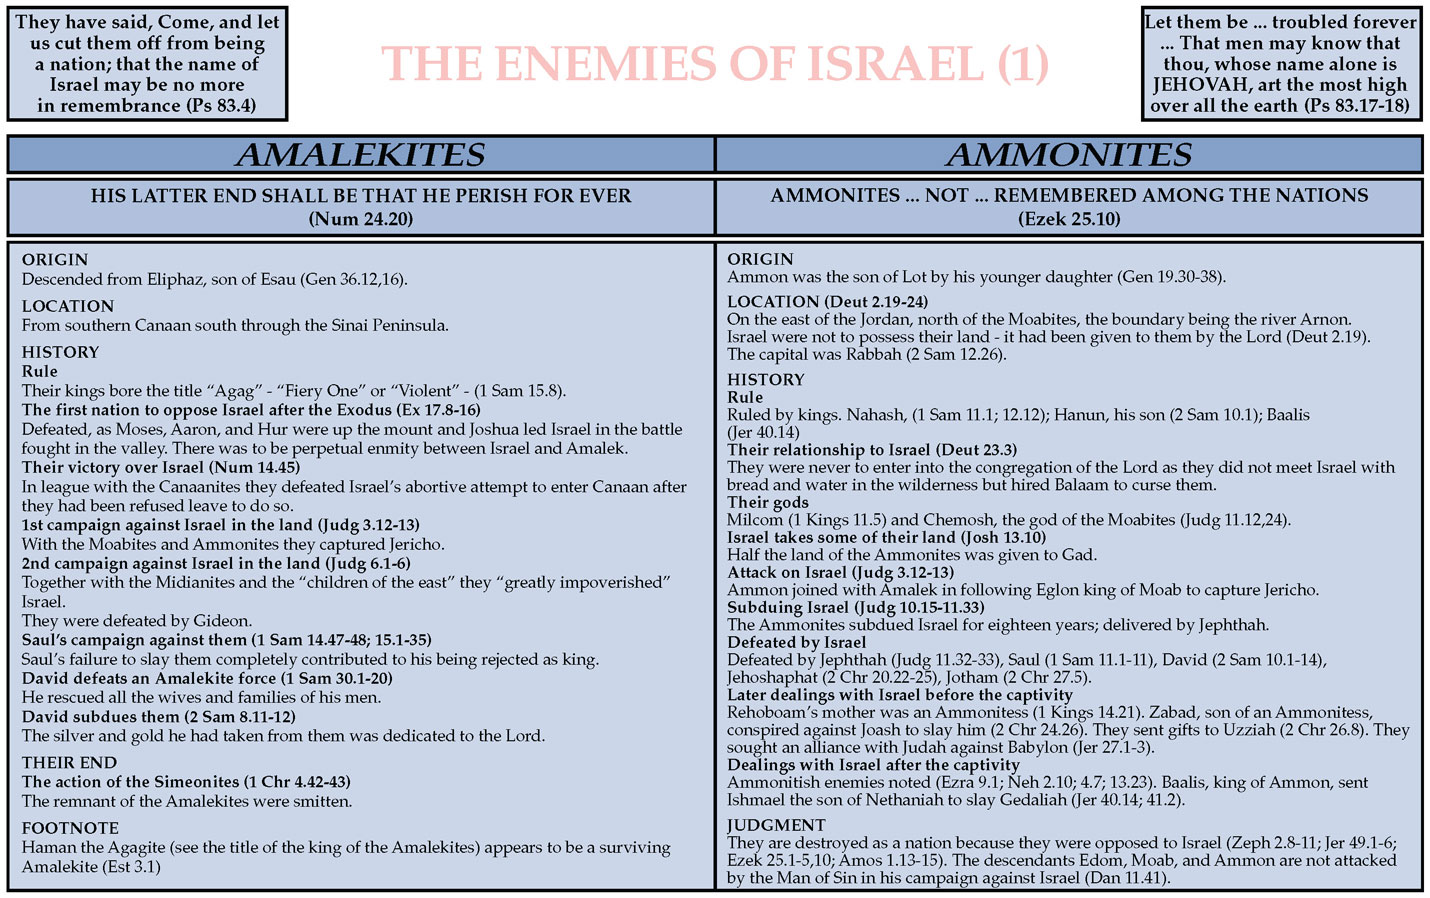
\includegraphics[scale=0.4, angle=90]{06OT-Joshua/References/3.EnemiesOfIsrael1.jpg}
\caption[Enemies of Israel 1]{Enemies of Israel 1}
\label{fig:Enemies of Israel 1}
\end{center}
\end{figure}

\newpage
\begin{figure}
\begin{center}
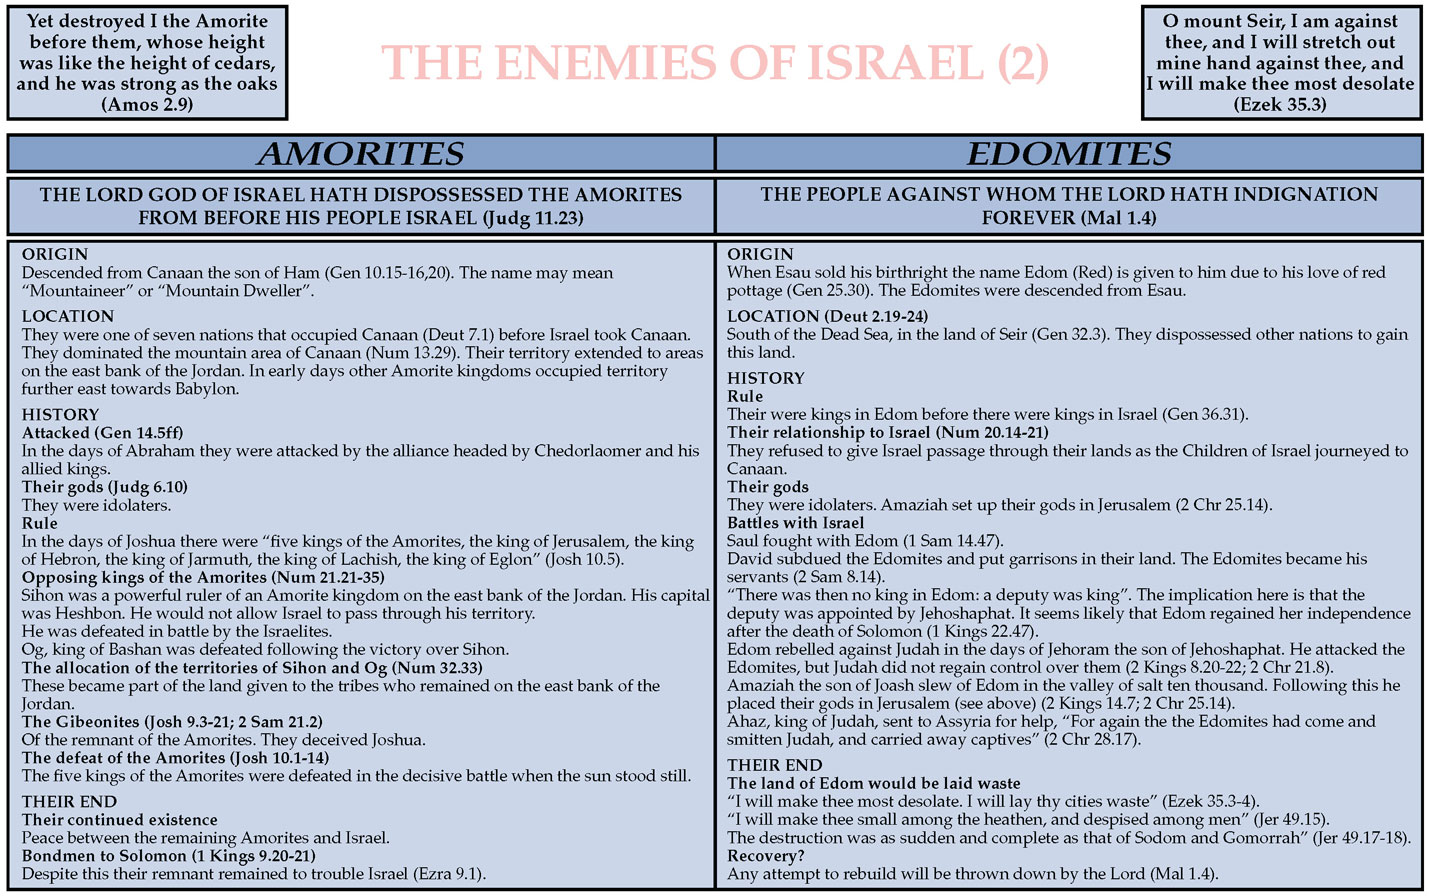
\includegraphics[scale=0.4, angle=90]{06OT-Joshua/References/4.EnemiesOfIsrael2.jpg}
\caption[Enemies of Israel 2]{Enemies of Israel 2}
\label{fig:Enemies of Israel 2}
\end{center}
\end{figure}

\newpage
\begin{figure}
\begin{center}
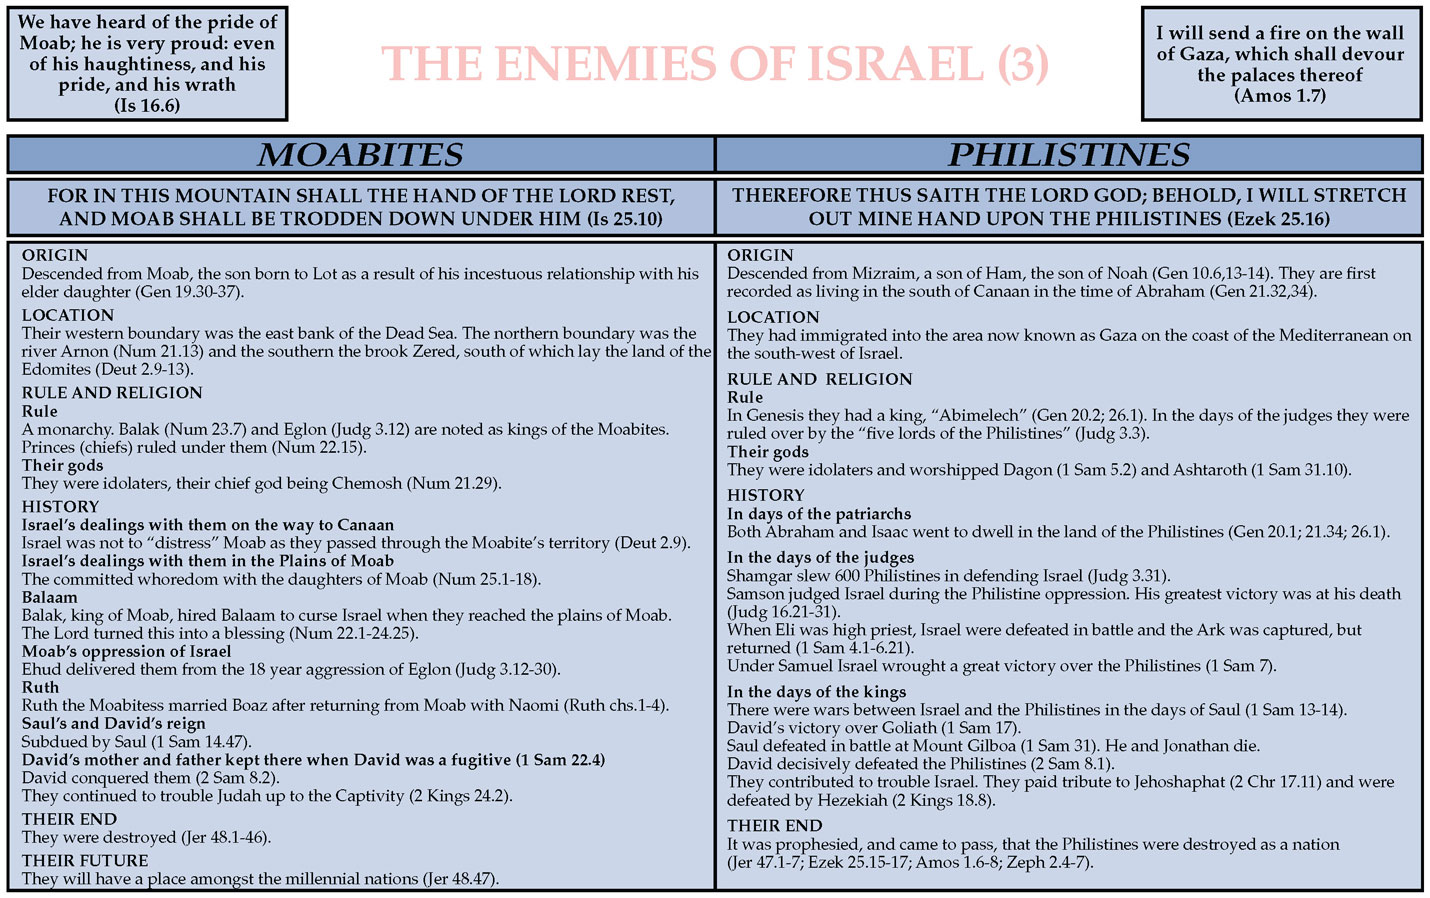
\includegraphics[scale=0.4, angle=90]{06OT-Joshua/References/5.EnemiesOfIsrael3.jpg}
\caption[Enemies of Israel 3]{Enemies of Israel 3}
\label{fig:Enemies of Israel 3}
\end{center}
\end{figure}

\newpage
\begin{figure}
\begin{center}
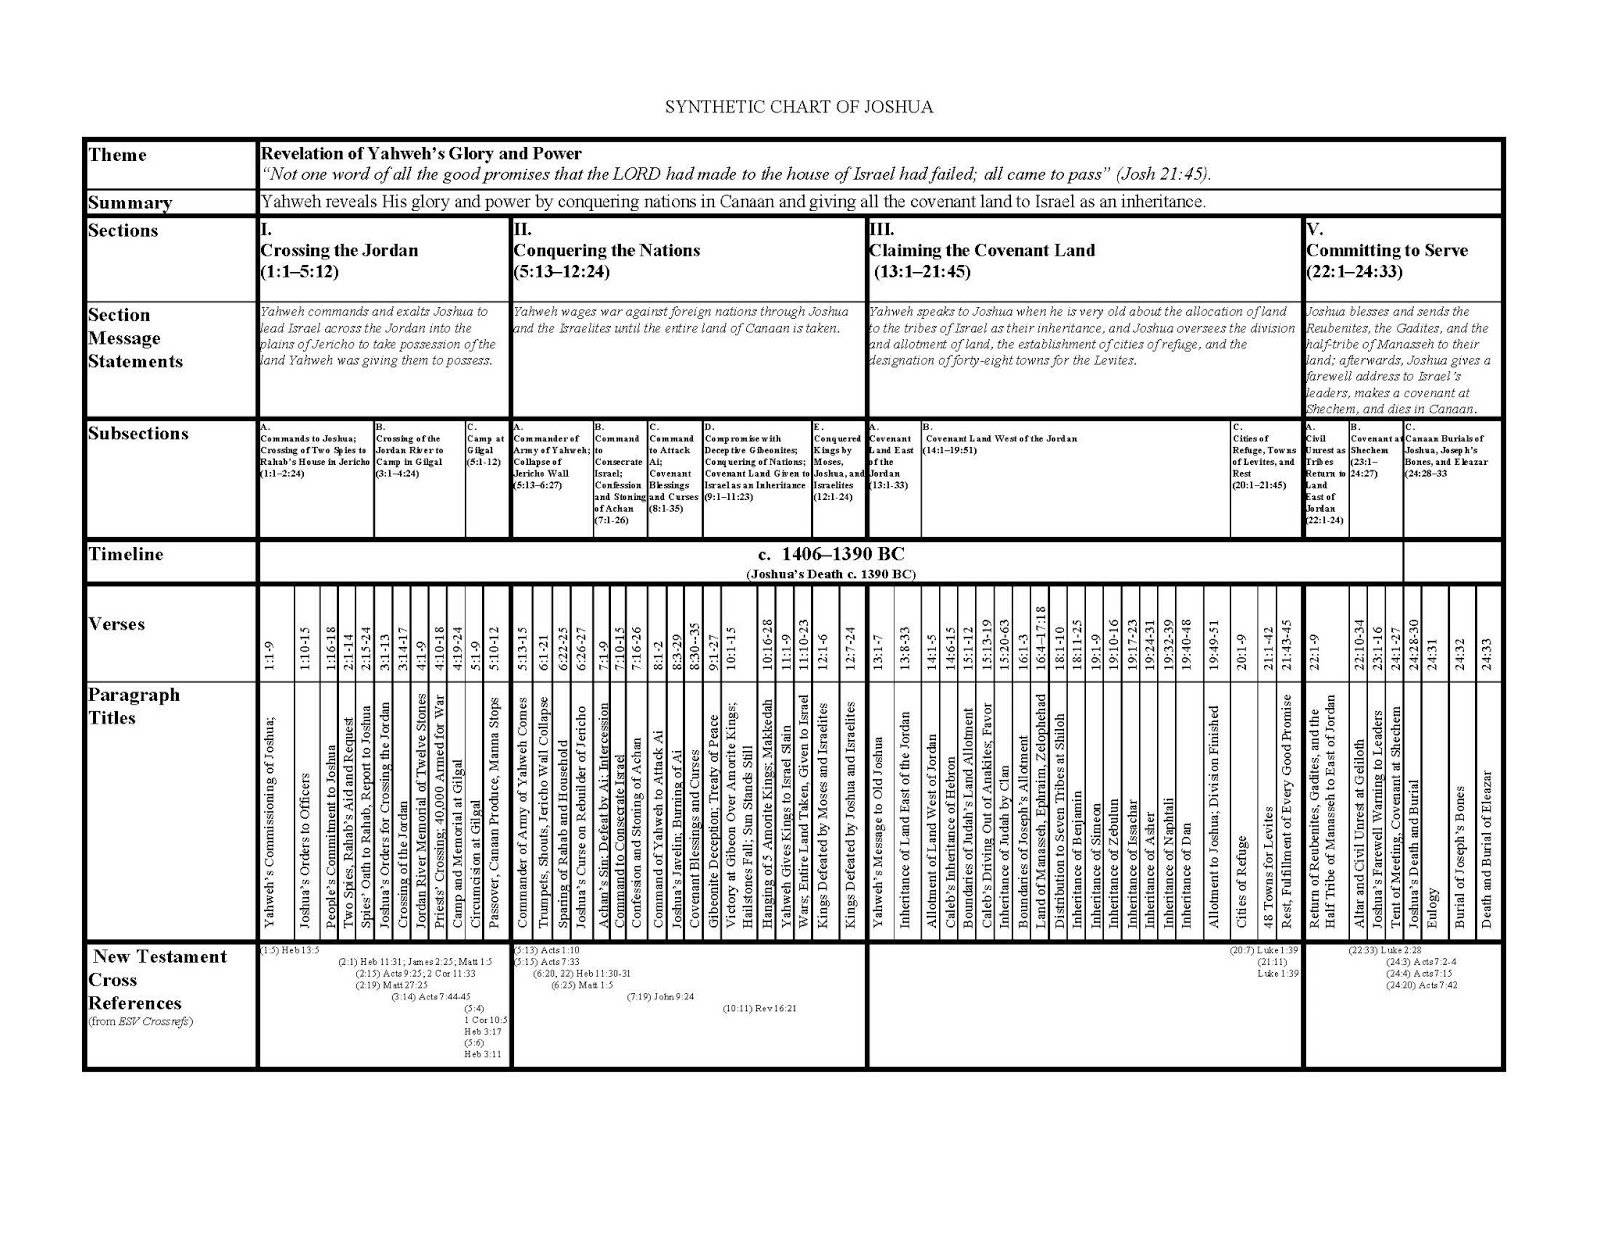
\includegraphics[scale=.4, angle=90]{06OT-Joshua/References/6.SyntheticChartofJoshua.jpg}
\caption[Synthetic Chart of Joshua]{Synthetic Chart of Joshua}
\label{fig:Synthetic Chart of Joshua}
\end{center}
\end{figure}


\newpage
\begin{figure}
\begin{center}
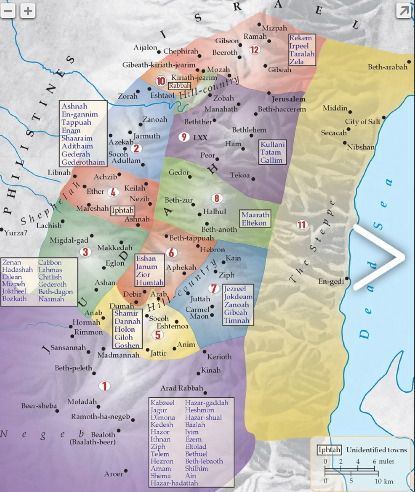
\includegraphics[scale=1, angle=0]{06OT-Joshua/References/7.WestSideOfDeadSea.jpg}
\caption[The West Side of the Dead Sea]{The West Side of the Dead Sea}
\label{fig:The West Side of the Dead Sea}
\end{center}
\end{figure}


\newpage
\begin{figure}
\begin{center}
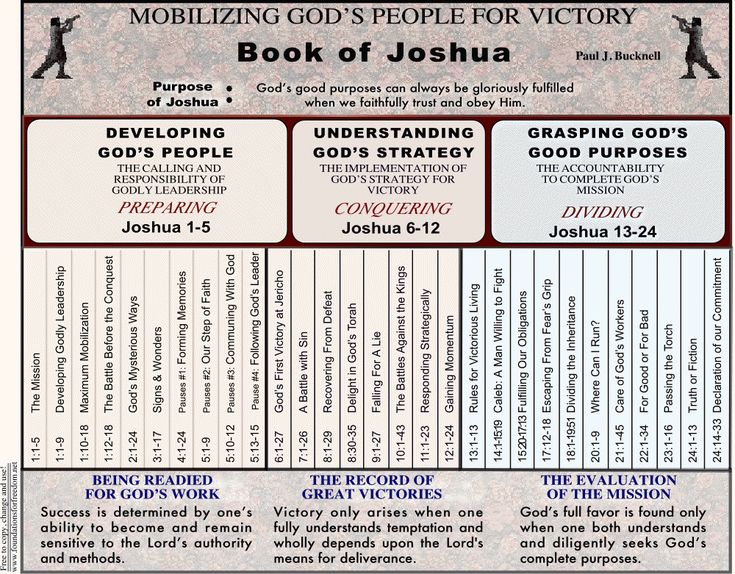
\includegraphics[scale=0.75, angle=90]{06OT-Joshua/References/8.Bucknell-Joshua.jpg}
\caption[Joshua from Bucknell]{Joshua from Bucknell}
\label{fig:Joshua from Bucknell}
\end{center}
\end{figure}


\newpage
\begin{figure}
\begin{center}
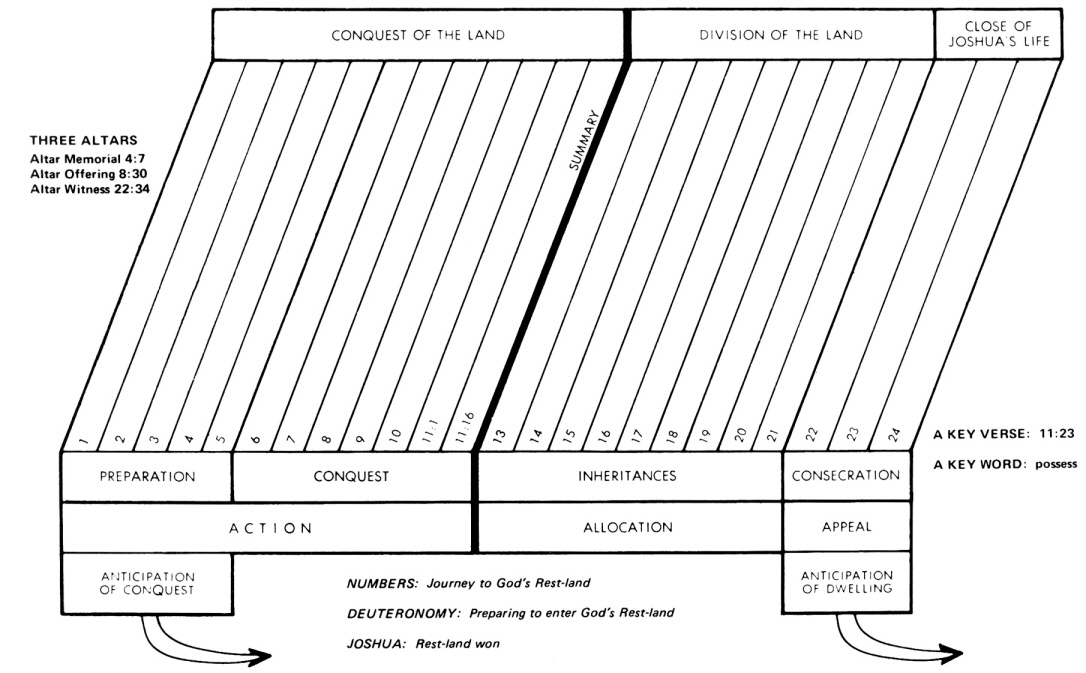
\includegraphics[scale=2, angle=90]{06OT-Joshua/References/9.Jensen-Joshua.png}
\caption[Joshua from Jensen]{Joshua from Jensen}
\label{fig:Joshua from Jensen}
\end{center}
\end{figure}


\newpage
\begin{figure}
\begin{center}
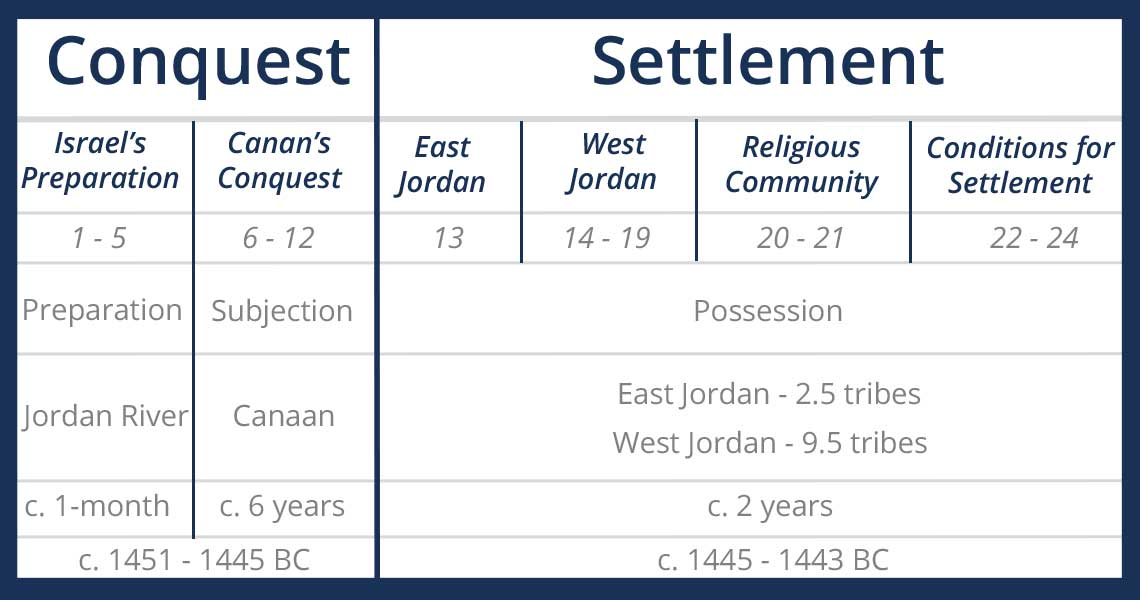
\includegraphics[scale=.5, angle=90]{06OT-Joshua/References/10.Bible-Brief-Joshua.jpg}
\caption[Bible Brief for Joshua]{Bible Brief for Joshua}
\label{fig:Bible Brief for Joshua}
\end{center}
\end{figure}

\newpage
\begin{figure}
\begin{center}
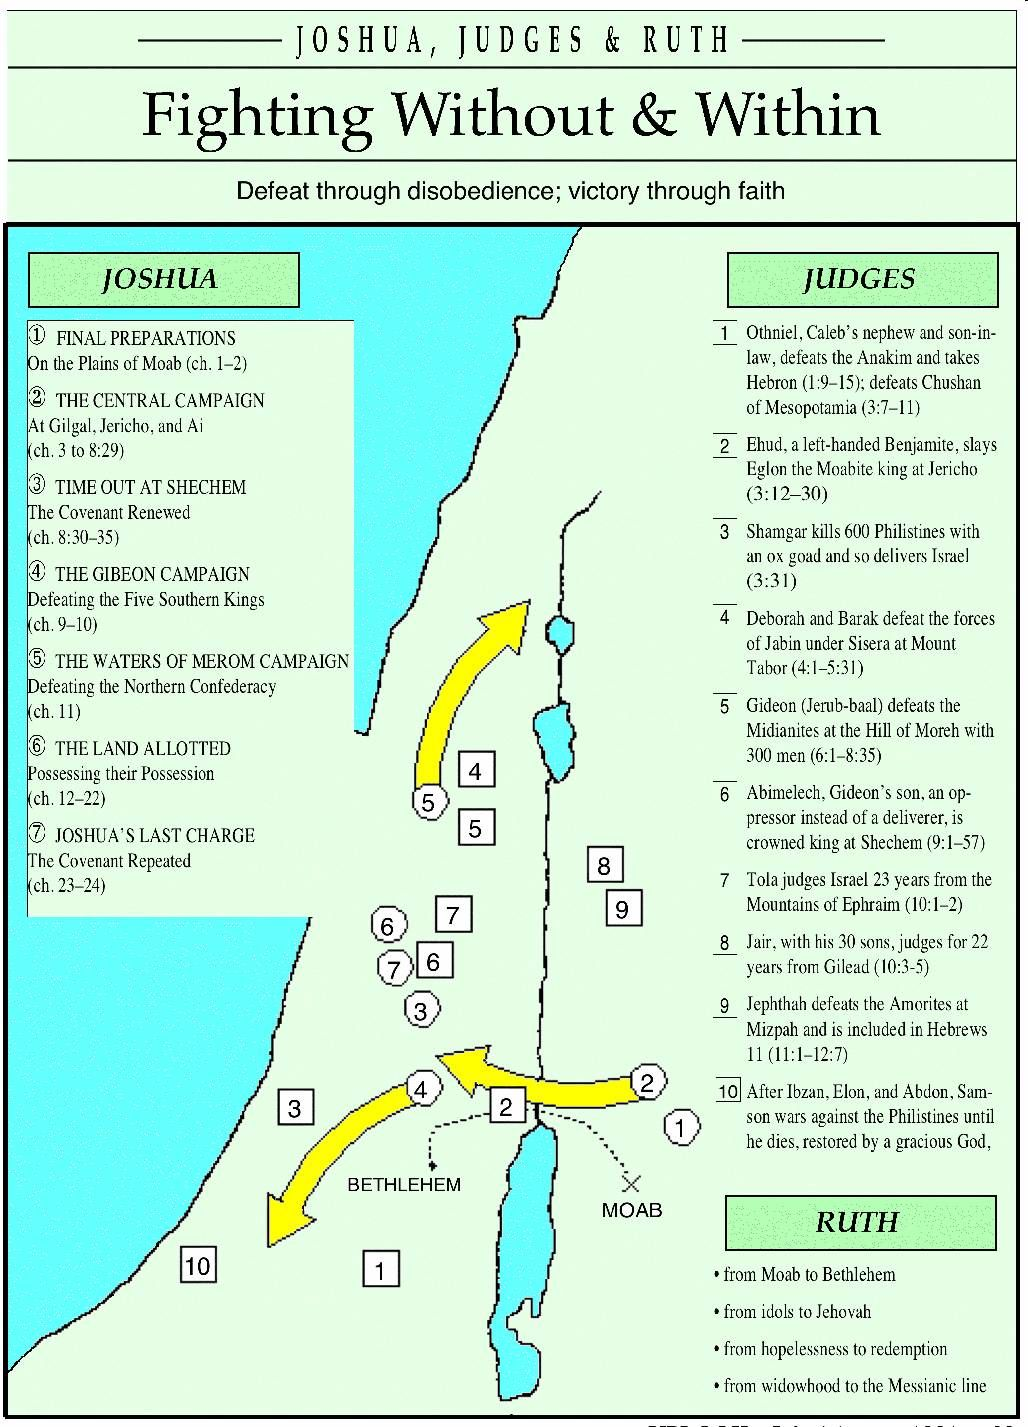
\includegraphics[scale=.5, angle=0]{06OT-Joshua/References/11.FightingInJoshuaAndJudges.jpg}
\caption[The Fighting in Joshua and Judges]{The Fighting in Joshua and Judges}
\label{fig:The Fighting in Joshua and Judges}
\end{center}
\end{figure}

\newpage
\begin{figure}
\begin{center}
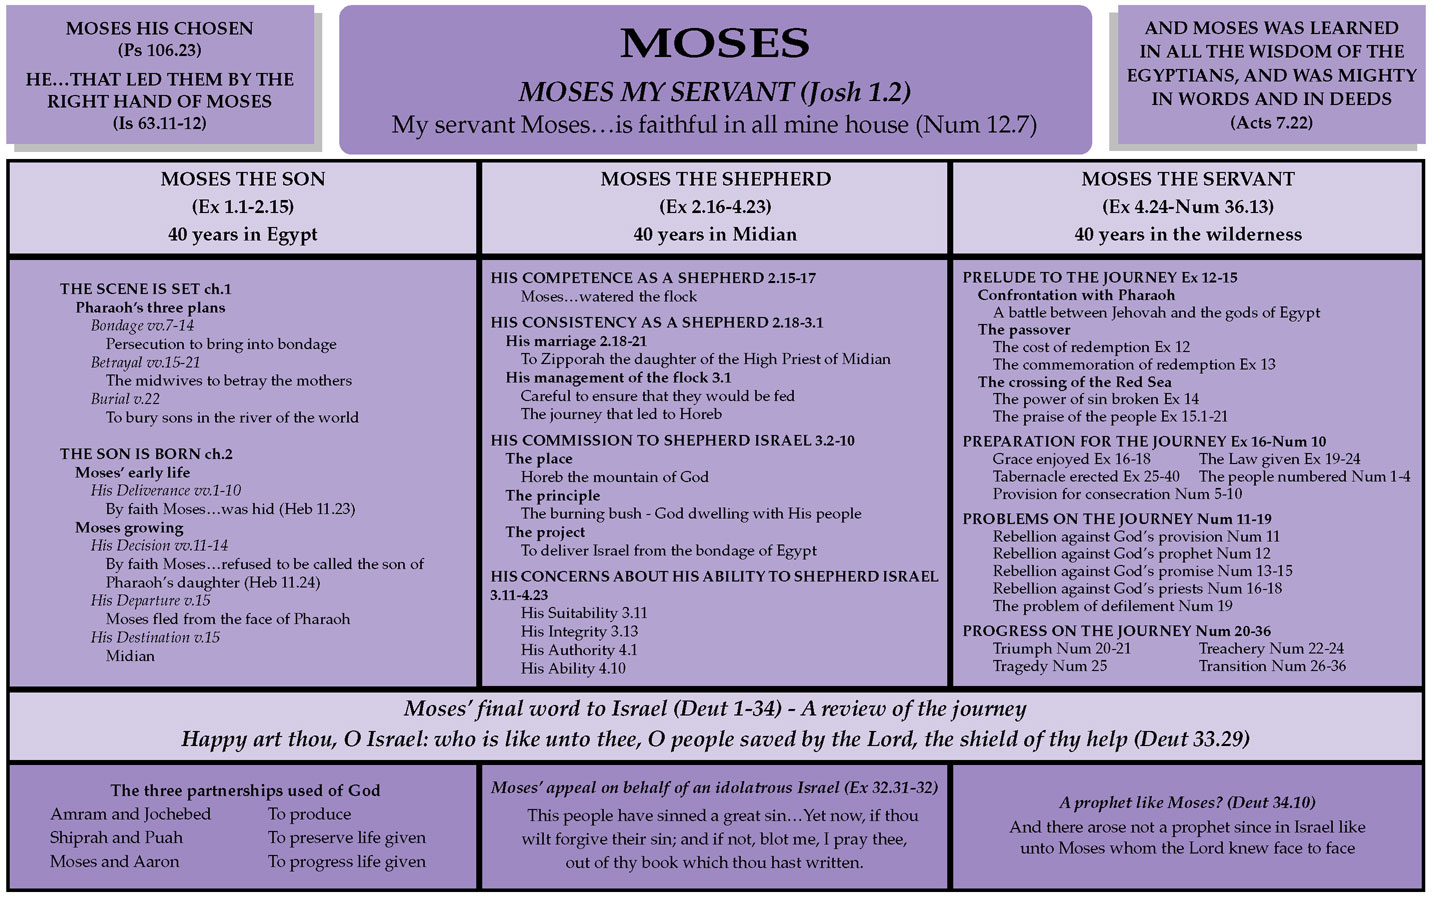
\includegraphics[scale=.4, angle=90]{06OT-Joshua/References/12.JohnGrantMoses.jpg}
\caption[Moses from John Grant]{Moses from John Grant}
\label{fig:Moses from John Grant}
\end{center}
\end{figure}








\chapter{Joshua 7}

\begin{figure}
  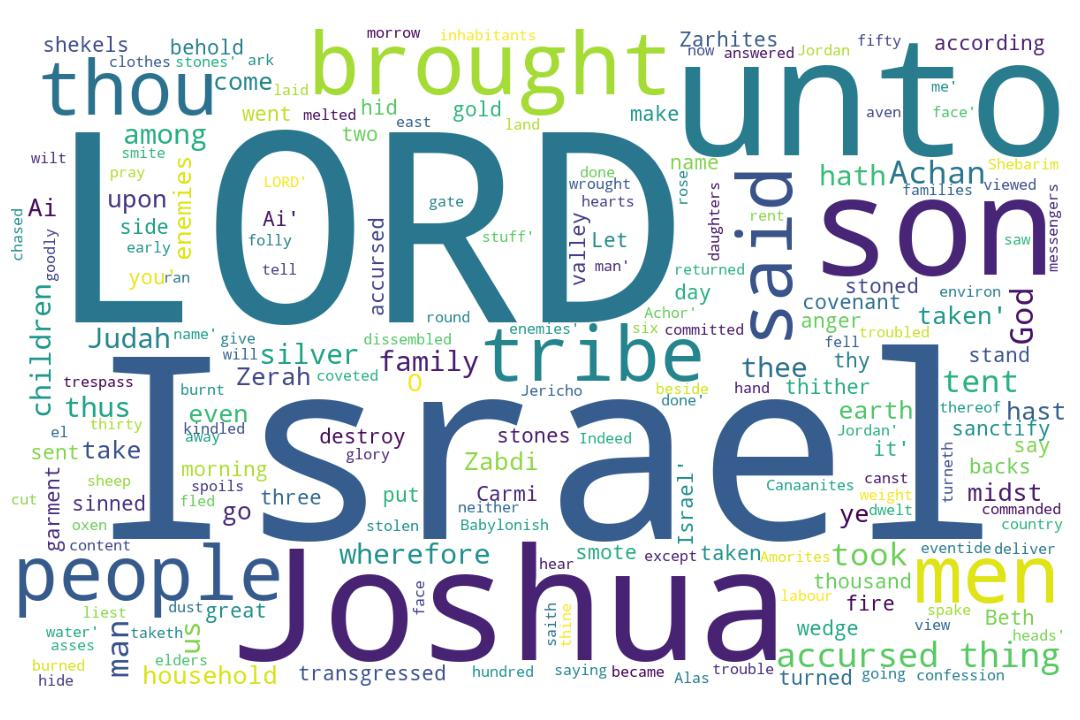
\includegraphics[width=\linewidth]{06OT-Joshua/Joshua7-WordCloud.jpg}
  \caption{Joshua 7 Word Cloud}
  \label{fig:Joshua 7Word Cloud}
\end{figure}

\marginpar{\scriptsize \centering \fcolorbox{bone}{lime}{\textbf{ACHIN FOR A BRUSIN'}}\\ (Joshua 7)

\begin{compactenum}[I.][8]

\item A \textbf{Pernicious Defiling}
\item A \textbf{Painful Defeat} \index[scripture]{Joshua!Jsh 07:04}  (Jsh 7:4) 
\item A \textbf{Public Declaration} \index[scripture]{Joshua!Jsh 07:20}  (Jsh 7:20) 
\item \textbf{Polluted Desire} \index[scripture]{Joshua!Jsh 07:21}  (Jsh 7:21) 
\item A \textbf{Personal Decision} \index[scripture]{Joshua!Jsh 07:21}  (Jsh 7:21) 
\item \textbf{Disproportionate Destruction} \index[scripture]{Joshua!Jsh 07:24}  (Jsh 7:24) 
\item A \textbf{Purifying Death} \index[scripture]{Joshua!Jsh 07:25}  (Jsh 7:25) 
\end{compactenum}}




\footnote{\textcolor[rgb]{0.00,0.25,0.00}{\hyperlink{TOC}{Return to end of Table of Contents.}}}\footnote{\href{https://audiobible.com/bible/joshua_7.html}{\textcolor[cmyk]{0.99998,1,0,0}{Joshua 7 Audio}}}\textcolor[cmyk]{0.99998,1,0,0}{But the children of Israel committed a trespass in the accursed thing: for Achan, the son of Carmi, the son of Zabdi, the son of Zerah, of the tribe of Judah, took of the accursed thing: and the anger of \fcolorbox{bone}{bone}{the LORD} was kindled against the children of Israel.}
[2] \textcolor[cmyk]{0.99998,1,0,0}{And Joshua sent men from Jericho to Ai, which \emph{is} beside Beth-aven, on the east side of Beth-el, and spake \fcolorbox{bone}{bone}{unto} \fcolorbox{bone}{bone}{them}, saying, Go up and view the country. And the men went up and viewed Ai.}
[3] \textcolor[cmyk]{0.99998,1,0,0}{And they returned to Joshua, and said \fcolorbox{bone}{bone}{unto} him, Let not all the people go up; but let about two or three thousand men go up and smite Ai; \emph{and} make not all the people to labour thither; for they \emph{are} \emph{but} few.}
[4] \textcolor[cmyk]{0.99998,1,0,0}{So there went up thither of the people about three thousand men: and they fled before the men of Ai.}
[5] \textcolor[cmyk]{0.99998,1,0,0}{And the men of Ai smote of \fcolorbox{bone}{bone}{them} about thirty and six men: for they chased \fcolorbox{bone}{bone}{them} \emph{from} before the gate \emph{even} \fcolorbox{bone}{bone}{unto} Shebarim, and smote \fcolorbox{bone}{bone}{them} in the going down: wherefore the hearts of the people melted, and became as water.}\\
\\
\P \textcolor[cmyk]{0.99998,1,0,0}{And Joshua rent his clothes, and fell to the earth upon his face before the ark of \fcolorbox{bone}{bone}{the LORD} until the eventide, he and the elders of Israel, and put dust upon their heads.}
[7] \textcolor[cmyk]{0.99998,1,0,0}{And Joshua said, Alas, O Lord GOD, wherefore hast thou at all brought this people over Jordan, to deliver us into the hand of the Amorites, to destroy us? would to God we had been content, and dwelt on the other side Jordan!}
[8] \textcolor[cmyk]{0.99998,1,0,0}{O Lord, what \fcolorbox{bone}{bone}{shall} I say, when Israel turneth their backs before their enemies!}
[9] \textcolor[cmyk]{0.99998,1,0,0}{For the Canaanites and all the inhabitants of the land \fcolorbox{bone}{bone}{shall} hear \emph{of} \emph{it}, and \fcolorbox{bone}{bone}{shall} environ us round, and cut off our name from the earth: and what wilt thou do \fcolorbox{bone}{bone}{unto} thy great name?}\\
\\
\P \textcolor[cmyk]{0.99998,1,0,0}{And \fcolorbox{bone}{bone}{the LORD} said \fcolorbox{bone}{bone}{unto} Joshua, Get thee up; wherefore liest thou thus upon thy face?}
[11] \textcolor[cmyk]{0.99998,1,0,0}{Israel hath sinned, and they have also transgressed my covenant which I commanded \fcolorbox{bone}{bone}{them}: for they have even taken of the accursed thing, and have also stolen, and dissembled also, and they have put \emph{it} even among their own stuff.}
[12] \textcolor[cmyk]{0.99998,1,0,0}{Therefore the children of Israel could not stand before their enemies, \emph{but} turned \emph{their} backs before their enemies, because they were accursed: neither will I be with you any more, except ye destroy the accursed from among you.}
[13] \textcolor[cmyk]{0.99998,1,0,0}{Up, sanctify the people, and say, Sanctify yourselves against to morrow: for thus saith \fcolorbox{bone}{bone}{the LORD} God of Israel, \emph{There} \emph{is} an accursed thing in the midst of thee, O Israel: thou canst not stand before thine enemies, until ye take away the accursed thing from among you.}
[14] \textcolor[cmyk]{0.99998,1,0,0}{In the morning therefore ye \fcolorbox{bone}{bone}{shall} be brought according to your tribes: and it \fcolorbox{bone}{bone}{shall} be, \emph{that} the tribe which \fcolorbox{bone}{bone}{the LORD} taketh \fcolorbox{bone}{bone}{shall} come according to the families \emph{thereof}; and the family which \fcolorbox{bone}{bone}{the LORD} \fcolorbox{bone}{bone}{shall} take \fcolorbox{bone}{bone}{shall} come by households; and the household which \fcolorbox{bone}{bone}{the LORD} \fcolorbox{bone}{bone}{shall} take \fcolorbox{bone}{bone}{shall} come man by man.}
[15] \textcolor[cmyk]{0.99998,1,0,0}{And it \fcolorbox{bone}{bone}{shall} be, \emph{that} he that is taken with the accursed thing \fcolorbox{bone}{bone}{shall} be burnt with fire, he and all that he hath: because he hath transgressed the covenant of \fcolorbox{bone}{bone}{the LORD}, and because he hath wrought folly in Israel.}\\
\\
\P \textcolor[cmyk]{0.99998,1,0,0}{So Joshua rose up early in the morning, and brought Israel by their tribes; and the tribe of Judah was taken:}
[17] \textcolor[cmyk]{0.99998,1,0,0}{And he brought the family of Judah; and he took the family of the Zarhites: and he brought the family of the Zarhites man by man; and Zabdi was taken:}
[18] \textcolor[cmyk]{0.99998,1,0,0}{And he brought his household man by man; and Achan, the son of Carmi, the son of Zabdi, the son of Zerah, of the tribe of Judah, was taken.}
[19] \textcolor[cmyk]{0.99998,1,0,0}{And Joshua said \fcolorbox{bone}{bone}{unto} Achan, My son, give, I pray thee, glory to \fcolorbox{bone}{bone}{the LORD} God of Israel, and make confession \fcolorbox{bone}{bone}{unto} him; and tell me now what thou hast done; hide \emph{it} not from me.}
[20] \textcolor[cmyk]{0.99998,1,0,0}{And Achan answered Joshua, and said, Indeed I have sinned against \fcolorbox{bone}{bone}{the LORD} God of Israel, and thus and thus have I done:}
[21] \textcolor[cmyk]{0.99998,1,0,0}{When I saw among the spoils a goodly Babylonish garment, and two hundred shekels of silver, and a wedge of gold of fifty shekels weight, then I coveted \fcolorbox{bone}{bone}{them}, and took \fcolorbox{bone}{bone}{them}; and, behold, they \emph{are} hid in the earth in the midst of my tent, and the silver under it.}\\
\\
\P \textcolor[cmyk]{0.99998,1,0,0}{So Joshua sent messengers, and they ran \fcolorbox{bone}{bone}{unto} the tent; and, behold, \emph{it} \emph{was} hid in his tent, and the silver under it.}
[23] \textcolor[cmyk]{0.99998,1,0,0}{And they took \fcolorbox{bone}{bone}{them} out of the midst of the tent, and brought \fcolorbox{bone}{bone}{them} \fcolorbox{bone}{bone}{unto} Joshua, and \fcolorbox{bone}{bone}{unto} all the children of Israel, and laid \fcolorbox{bone}{bone}{them} out before \fcolorbox{bone}{bone}{the LORD}.}
[24] \textcolor[cmyk]{0.99998,1,0,0}{And Joshua, and all Israel with him, took Achan the son of Zerah, and the silver, and the garment, and the wedge of gold, and his sons, and his daughters, and his oxen, and his asses, and his sheep, and his tent, and all that he had: and they brought \fcolorbox{bone}{bone}{them} \fcolorbox{bone}{bone}{unto} the valley of Achor.}
[25] \textcolor[cmyk]{0.99998,1,0,0}{And Joshua said, Why hast thou troubled us? \fcolorbox{bone}{bone}{the LORD} \fcolorbox{bone}{bone}{shall} trouble thee this day. And all Israel stoned him with stones, and burned \fcolorbox{bone}{bone}{them} with fire, after they had stoned \fcolorbox{bone}{bone}{them} with stones.}
[26] \textcolor[cmyk]{0.99998,1,0,0}{And they raised over him a great heap of stones \fcolorbox{bone}{bone}{unto} this day. So \fcolorbox{bone}{bone}{the LORD} turned from the fierceness of his anger. Wherefore the name of that place was called, The valley of Achor, \fcolorbox{bone}{bone}{unto} this day.}
]       



\index[NWIV]{49!Joshua!Jos 7:1}\index[AWIP]{But!Joshua!Jos 7:1}\index[AWIP]{the!Joshua!Jos 7:1}\index[AWIP]{the!Joshua!Jos 7:1 (2)}\index[AWIP]{the!Joshua!Jos 7:1 (3)}\index[AWIP]{the!Joshua!Jos 7:1 (4)}\index[AWIP]{the!Joshua!Jos 7:1 (5)}\index[AWIP]{the!Joshua!Jos 7:1 (6)}\index[AWIP]{the!Joshua!Jos 7:1 (7)}\index[AWIP]{the!Joshua!Jos 7:1 (8)}\index[AWIP]{the!Joshua!Jos 7:1 (9)}\index[AWIP]{the!Joshua!Jos 7:1 (10)}\index[AWIP]{children!Joshua!Jos 7:1}\index[AWIP]{children!Joshua!Jos 7:1 (2)}\index[AWIP]{of!Joshua!Jos 7:1}\index[AWIP]{of!Joshua!Jos 7:1 (2)}\index[AWIP]{of!Joshua!Jos 7:1 (3)}\index[AWIP]{of!Joshua!Jos 7:1 (4)}\index[AWIP]{of!Joshua!Jos 7:1 (5)}\index[AWIP]{of!Joshua!Jos 7:1 (6)}\index[AWIP]{of!Joshua!Jos 7:1 (7)}\index[AWIP]{of!Joshua!Jos 7:1 (8)}\index[AWIP]{of!Joshua!Jos 7:1 (9)}\index[AWIP]{Israel!Joshua!Jos 7:1}\index[AWIP]{Israel!Joshua!Jos 7:1 (2)}\index[AWIP]{committed!Joshua!Jos 7:1}\index[AWIP]{a!Joshua!Jos 7:1}\index[AWIP]{trespass!Joshua!Jos 7:1}\index[AWIP]{in!Joshua!Jos 7:1}\index[AWIP]{accursed!Joshua!Jos 7:1}\index[AWIP]{accursed!Joshua!Jos 7:1 (2)}\index[AWIP]{thing!Joshua!Jos 7:1}\index[AWIP]{thing!Joshua!Jos 7:1 (2)}\index[AWIP]{for!Joshua!Jos 7:1}\index[AWIP]{Achan!Joshua!Jos 7:1}\index[AWIP]{son!Joshua!Jos 7:1}\index[AWIP]{son!Joshua!Jos 7:1 (2)}\index[AWIP]{son!Joshua!Jos 7:1 (3)}\index[AWIP]{Carmi!Joshua!Jos 7:1}\index[AWIP]{Zabdi!Joshua!Jos 7:1}\index[AWIP]{Zerah!Joshua!Jos 7:1}\index[AWIP]{tribe!Joshua!Jos 7:1}\index[AWIP]{Judah!Joshua!Jos 7:1}\index[AWIP]{took!Joshua!Jos 7:1}\index[AWIP]{and!Joshua!Jos 7:1}\index[AWIP]{anger!Joshua!Jos 7:1}\index[AWIP]{LORD!Joshua!Jos 7:1}\index[AWIP]{was!Joshua!Jos 7:1}\index[AWIP]{kindled!Joshua!Jos 7:1}\index[AWIP]{against!Joshua!Jos 7:1}

\index[NWIV]{37!Joshua!Jos 7:2}\index[AWIP]{And!Joshua!Jos 7:2}\index[AWIP]{And!Joshua!Jos 7:2 (2)}\index[AWIP]{Joshua!Joshua!Jos 7:2}\index[AWIP]{sent!Joshua!Jos 7:2}\index[AWIP]{men!Joshua!Jos 7:2}\index[AWIP]{men!Joshua!Jos 7:2 (2)}\index[AWIP]{from!Joshua!Jos 7:2}\index[AWIP]{Jericho!Joshua!Jos 7:2}\index[AWIP]{to!Joshua!Jos 7:2}\index[AWIP]{Ai!Joshua!Jos 7:2}\index[AWIP]{Ai!Joshua!Jos 7:2 (2)}\index[AWIP]{which!Joshua!Jos 7:2}\index[AWIP]{\emph{is}!Joshua!Jos 7:2}\index[AWIP]{beside!Joshua!Jos 7:2}\index[AWIP]{Beth-aven!Joshua!Jos 7:2}\index[AWIP]{on!Joshua!Jos 7:2}\index[AWIP]{the!Joshua!Jos 7:2}\index[AWIP]{the!Joshua!Jos 7:2 (2)}\index[AWIP]{the!Joshua!Jos 7:2 (3)}\index[AWIP]{east!Joshua!Jos 7:2}\index[AWIP]{side!Joshua!Jos 7:2}\index[AWIP]{of!Joshua!Jos 7:2}\index[AWIP]{Beth-el!Joshua!Jos 7:2}\index[AWIP]{and!Joshua!Jos 7:2}\index[AWIP]{and!Joshua!Jos 7:2 (2)}\index[AWIP]{and!Joshua!Jos 7:2 (3)}\index[AWIP]{spake!Joshua!Jos 7:2}\index[AWIP]{unto!Joshua!Jos 7:2}\index[AWIP]{them!Joshua!Jos 7:2}\index[AWIP]{saying!Joshua!Jos 7:2}\index[AWIP]{Go!Joshua!Jos 7:2}\index[AWIP]{up!Joshua!Jos 7:2}\index[AWIP]{up!Joshua!Jos 7:2 (2)}\index[AWIP]{view!Joshua!Jos 7:2}\index[AWIP]{country!Joshua!Jos 7:2}\index[AWIP]{went!Joshua!Jos 7:2}\index[AWIP]{viewed!Joshua!Jos 7:2}\index[AWIP]{\emph{is}!Joshua!Jos 7:2}

\index[NWIV]{43!Joshua!Jos 7:3}\index[AWIP]{And!Joshua!Jos 7:3}\index[AWIP]{they!Joshua!Jos 7:3}\index[AWIP]{they!Joshua!Jos 7:3 (2)}\index[AWIP]{returned!Joshua!Jos 7:3}\index[AWIP]{to!Joshua!Jos 7:3}\index[AWIP]{to!Joshua!Jos 7:3 (2)}\index[AWIP]{Joshua!Joshua!Jos 7:3}\index[AWIP]{and!Joshua!Jos 7:3}\index[AWIP]{and!Joshua!Jos 7:3 (2)}\index[AWIP]{said!Joshua!Jos 7:3}\index[AWIP]{unto!Joshua!Jos 7:3}\index[AWIP]{him!Joshua!Jos 7:3}\index[AWIP]{Let!Joshua!Jos 7:3}\index[AWIP]{not!Joshua!Jos 7:3}\index[AWIP]{not!Joshua!Jos 7:3 (2)}\index[AWIP]{all!Joshua!Jos 7:3}\index[AWIP]{all!Joshua!Jos 7:3 (2)}\index[AWIP]{the!Joshua!Jos 7:3}\index[AWIP]{the!Joshua!Jos 7:3 (2)}\index[AWIP]{people!Joshua!Jos 7:3}\index[AWIP]{people!Joshua!Jos 7:3 (2)}\index[AWIP]{go!Joshua!Jos 7:3}\index[AWIP]{go!Joshua!Jos 7:3 (2)}\index[AWIP]{up!Joshua!Jos 7:3}\index[AWIP]{up!Joshua!Jos 7:3 (2)}\index[AWIP]{but!Joshua!Jos 7:3}\index[AWIP]{let!Joshua!Jos 7:3}\index[AWIP]{about!Joshua!Jos 7:3}\index[AWIP]{two!Joshua!Jos 7:3}\index[AWIP]{or!Joshua!Jos 7:3}\index[AWIP]{three!Joshua!Jos 7:3}\index[AWIP]{thousand!Joshua!Jos 7:3}\index[AWIP]{men!Joshua!Jos 7:3}\index[AWIP]{smite!Joshua!Jos 7:3}\index[AWIP]{Ai!Joshua!Jos 7:3}\index[AWIP]{\emph{and}!Joshua!Jos 7:3}\index[AWIP]{make!Joshua!Jos 7:3}\index[AWIP]{labour!Joshua!Jos 7:3}\index[AWIP]{thither!Joshua!Jos 7:3}\index[AWIP]{for!Joshua!Jos 7:3}\index[AWIP]{\emph{are}!Joshua!Jos 7:3}\index[AWIP]{\emph{but}!Joshua!Jos 7:3}\index[AWIP]{few!Joshua!Jos 7:3}\index[AWIP]{\emph{and}!Joshua!Jos 7:3}\index[AWIP]{\emph{are}!Joshua!Jos 7:3}\index[AWIP]{\emph{but}!Joshua!Jos 7:3}

\index[NWIV]{20!Joshua!Jos 7:4}\index[AWIP]{So!Joshua!Jos 7:4}\index[AWIP]{there!Joshua!Jos 7:4}\index[AWIP]{went!Joshua!Jos 7:4}\index[AWIP]{up!Joshua!Jos 7:4}\index[AWIP]{thither!Joshua!Jos 7:4}\index[AWIP]{of!Joshua!Jos 7:4}\index[AWIP]{of!Joshua!Jos 7:4 (2)}\index[AWIP]{the!Joshua!Jos 7:4}\index[AWIP]{the!Joshua!Jos 7:4 (2)}\index[AWIP]{people!Joshua!Jos 7:4}\index[AWIP]{about!Joshua!Jos 7:4}\index[AWIP]{three!Joshua!Jos 7:4}\index[AWIP]{thousand!Joshua!Jos 7:4}\index[AWIP]{men!Joshua!Jos 7:4}\index[AWIP]{men!Joshua!Jos 7:4 (2)}\index[AWIP]{and!Joshua!Jos 7:4}\index[AWIP]{they!Joshua!Jos 7:4}\index[AWIP]{fled!Joshua!Jos 7:4}\index[AWIP]{before!Joshua!Jos 7:4}\index[AWIP]{Ai!Joshua!Jos 7:4}

\index[NWIV]{42!Joshua!Jos 7:5}\index[AWIP]{And!Joshua!Jos 7:5}\index[AWIP]{the!Joshua!Jos 7:5}\index[AWIP]{the!Joshua!Jos 7:5 (2)}\index[AWIP]{the!Joshua!Jos 7:5 (3)}\index[AWIP]{the!Joshua!Jos 7:5 (4)}\index[AWIP]{the!Joshua!Jos 7:5 (5)}\index[AWIP]{men!Joshua!Jos 7:5}\index[AWIP]{men!Joshua!Jos 7:5 (2)}\index[AWIP]{of!Joshua!Jos 7:5}\index[AWIP]{of!Joshua!Jos 7:5 (2)}\index[AWIP]{of!Joshua!Jos 7:5 (3)}\index[AWIP]{Ai!Joshua!Jos 7:5}\index[AWIP]{smote!Joshua!Jos 7:5}\index[AWIP]{smote!Joshua!Jos 7:5 (2)}\index[AWIP]{them!Joshua!Jos 7:5}\index[AWIP]{them!Joshua!Jos 7:5 (2)}\index[AWIP]{them!Joshua!Jos 7:5 (3)}\index[AWIP]{about!Joshua!Jos 7:5}\index[AWIP]{thirty!Joshua!Jos 7:5}\index[AWIP]{and!Joshua!Jos 7:5}\index[AWIP]{and!Joshua!Jos 7:5 (2)}\index[AWIP]{and!Joshua!Jos 7:5 (3)}\index[AWIP]{six!Joshua!Jos 7:5}\index[AWIP]{for!Joshua!Jos 7:5}\index[AWIP]{they!Joshua!Jos 7:5}\index[AWIP]{chased!Joshua!Jos 7:5}\index[AWIP]{\emph{from}!Joshua!Jos 7:5}\index[AWIP]{before!Joshua!Jos 7:5}\index[AWIP]{gate!Joshua!Jos 7:5}\index[AWIP]{\emph{even}!Joshua!Jos 7:5}\index[AWIP]{unto!Joshua!Jos 7:5}\index[AWIP]{Shebarim!Joshua!Jos 7:5}\index[AWIP]{in!Joshua!Jos 7:5}\index[AWIP]{going!Joshua!Jos 7:5}\index[AWIP]{down!Joshua!Jos 7:5}\index[AWIP]{wherefore!Joshua!Jos 7:5}\index[AWIP]{hearts!Joshua!Jos 7:5}\index[AWIP]{people!Joshua!Jos 7:5}\index[AWIP]{melted!Joshua!Jos 7:5}\index[AWIP]{became!Joshua!Jos 7:5}\index[AWIP]{as!Joshua!Jos 7:5}\index[AWIP]{water!Joshua!Jos 7:5}\index[AWIP]{\emph{from}!Joshua!Jos 7:5}\index[AWIP]{\emph{even}!Joshua!Jos 7:5}

\index[NWIV]{34!Joshua!Jos 7:6}\index[AWIP]{And!Joshua!Jos 7:6}\index[AWIP]{Joshua!Joshua!Jos 7:6}\index[AWIP]{rent!Joshua!Jos 7:6}\index[AWIP]{his!Joshua!Jos 7:6}\index[AWIP]{his!Joshua!Jos 7:6 (2)}\index[AWIP]{clothes!Joshua!Jos 7:6}\index[AWIP]{and!Joshua!Jos 7:6}\index[AWIP]{and!Joshua!Jos 7:6 (2)}\index[AWIP]{and!Joshua!Jos 7:6 (3)}\index[AWIP]{fell!Joshua!Jos 7:6}\index[AWIP]{to!Joshua!Jos 7:6}\index[AWIP]{the!Joshua!Jos 7:6}\index[AWIP]{the!Joshua!Jos 7:6 (2)}\index[AWIP]{the!Joshua!Jos 7:6 (3)}\index[AWIP]{the!Joshua!Jos 7:6 (4)}\index[AWIP]{the!Joshua!Jos 7:6 (5)}\index[AWIP]{earth!Joshua!Jos 7:6}\index[AWIP]{upon!Joshua!Jos 7:6}\index[AWIP]{upon!Joshua!Jos 7:6 (2)}\index[AWIP]{face!Joshua!Jos 7:6}\index[AWIP]{before!Joshua!Jos 7:6}\index[AWIP]{ark!Joshua!Jos 7:6}\index[AWIP]{of!Joshua!Jos 7:6}\index[AWIP]{of!Joshua!Jos 7:6 (2)}\index[AWIP]{LORD!Joshua!Jos 7:6}\index[AWIP]{until!Joshua!Jos 7:6}\index[AWIP]{eventide!Joshua!Jos 7:6}\index[AWIP]{he!Joshua!Jos 7:6}\index[AWIP]{elders!Joshua!Jos 7:6}\index[AWIP]{Israel!Joshua!Jos 7:6}\index[AWIP]{put!Joshua!Jos 7:6}\index[AWIP]{dust!Joshua!Jos 7:6}\index[AWIP]{their!Joshua!Jos 7:6}\index[AWIP]{heads!Joshua!Jos 7:6}

\index[NWIV]{43!Joshua!Jos 7:7}\index[AWIP]{And!Joshua!Jos 7:7}\index[AWIP]{Joshua!Joshua!Jos 7:7}\index[AWIP]{said!Joshua!Jos 7:7}\index[AWIP]{Alas!Joshua!Jos 7:7}\index[AWIP]{O!Joshua!Jos 7:7}\index[AWIP]{Lord!Joshua!Jos 7:7}\index[AWIP]{GOD!Joshua!Jos 7:7}\index[AWIP]{wherefore!Joshua!Jos 7:7}\index[AWIP]{hast!Joshua!Jos 7:7}\index[AWIP]{thou!Joshua!Jos 7:7}\index[AWIP]{at!Joshua!Jos 7:7}\index[AWIP]{all!Joshua!Jos 7:7}\index[AWIP]{brought!Joshua!Jos 7:7}\index[AWIP]{this!Joshua!Jos 7:7}\index[AWIP]{people!Joshua!Jos 7:7}\index[AWIP]{over!Joshua!Jos 7:7}\index[AWIP]{Jordan!Joshua!Jos 7:7}\index[AWIP]{to!Joshua!Jos 7:7}\index[AWIP]{to!Joshua!Jos 7:7 (2)}\index[AWIP]{to!Joshua!Jos 7:7 (3)}\index[AWIP]{deliver!Joshua!Jos 7:7}\index[AWIP]{us!Joshua!Jos 7:7}\index[AWIP]{into!Joshua!Jos 7:7}\index[AWIP]{the!Joshua!Jos 7:7}\index[AWIP]{the!Joshua!Jos 7:7 (2)}\index[AWIP]{the!Joshua!Jos 7:7 (3)}\index[AWIP]{hand!Joshua!Jos 7:7}\index[AWIP]{of!Joshua!Jos 7:7}\index[AWIP]{Amorites!Joshua!Jos 7:7}\index[AWIP]{destroy!Joshua!Jos 7:7}\index[AWIP]{us?!Joshua!Jos 7:7}\index[AWIP]{would!Joshua!Jos 7:7}\index[AWIP]{God!Joshua!Jos 7:7}\index[AWIP]{we!Joshua!Jos 7:7}\index[AWIP]{had!Joshua!Jos 7:7}\index[AWIP]{been!Joshua!Jos 7:7}\index[AWIP]{content!Joshua!Jos 7:7}\index[AWIP]{and!Joshua!Jos 7:7}\index[AWIP]{dwelt!Joshua!Jos 7:7}\index[AWIP]{on!Joshua!Jos 7:7}\index[AWIP]{other!Joshua!Jos 7:7}\index[AWIP]{side!Joshua!Jos 7:7}\index[AWIP]{Jordan!!Joshua!Jos 7:7}

\index[NWIV]{14!Joshua!Jos 7:8}\index[AWIP]{O!Joshua!Jos 7:8}\index[AWIP]{Lord!Joshua!Jos 7:8}\index[AWIP]{what!Joshua!Jos 7:8}\index[AWIP]{shall!Joshua!Jos 7:8}\index[AWIP]{I!Joshua!Jos 7:8}\index[AWIP]{say!Joshua!Jos 7:8}\index[AWIP]{when!Joshua!Jos 7:8}\index[AWIP]{Israel!Joshua!Jos 7:8}\index[AWIP]{turneth!Joshua!Jos 7:8}\index[AWIP]{their!Joshua!Jos 7:8}\index[AWIP]{their!Joshua!Jos 7:8 (2)}\index[AWIP]{backs!Joshua!Jos 7:8}\index[AWIP]{before!Joshua!Jos 7:8}\index[AWIP]{enemies!!Joshua!Jos 7:8}

\index[NWIV]{36!Joshua!Jos 7:9}\index[AWIP]{For!Joshua!Jos 7:9}\index[AWIP]{the!Joshua!Jos 7:9}\index[AWIP]{the!Joshua!Jos 7:9 (2)}\index[AWIP]{the!Joshua!Jos 7:9 (3)}\index[AWIP]{the!Joshua!Jos 7:9 (4)}\index[AWIP]{Canaanites!Joshua!Jos 7:9}\index[AWIP]{and!Joshua!Jos 7:9}\index[AWIP]{and!Joshua!Jos 7:9 (2)}\index[AWIP]{and!Joshua!Jos 7:9 (3)}\index[AWIP]{and!Joshua!Jos 7:9 (4)}\index[AWIP]{all!Joshua!Jos 7:9}\index[AWIP]{inhabitants!Joshua!Jos 7:9}\index[AWIP]{of!Joshua!Jos 7:9}\index[AWIP]{land!Joshua!Jos 7:9}\index[AWIP]{shall!Joshua!Jos 7:9}\index[AWIP]{shall!Joshua!Jos 7:9 (2)}\index[AWIP]{hear!Joshua!Jos 7:9}\index[AWIP]{\emph{of}!Joshua!Jos 7:9}\index[AWIP]{\emph{it}!Joshua!Jos 7:9}\index[AWIP]{environ!Joshua!Jos 7:9}\index[AWIP]{us!Joshua!Jos 7:9}\index[AWIP]{round!Joshua!Jos 7:9}\index[AWIP]{cut!Joshua!Jos 7:9}\index[AWIP]{off!Joshua!Jos 7:9}\index[AWIP]{our!Joshua!Jos 7:9}\index[AWIP]{name!Joshua!Jos 7:9}\index[AWIP]{from!Joshua!Jos 7:9}\index[AWIP]{earth!Joshua!Jos 7:9}\index[AWIP]{what!Joshua!Jos 7:9}\index[AWIP]{wilt!Joshua!Jos 7:9}\index[AWIP]{thou!Joshua!Jos 7:9}\index[AWIP]{do!Joshua!Jos 7:9}\index[AWIP]{unto!Joshua!Jos 7:9}\index[AWIP]{thy!Joshua!Jos 7:9}\index[AWIP]{great!Joshua!Jos 7:9}\index[AWIP]{name?!Joshua!Jos 7:9}\index[AWIP]{\emph{of}!Joshua!Jos 7:9}\index[AWIP]{\emph{it}!Joshua!Jos 7:9}

\index[NWIV]{16!Joshua!Jos 7:10}\index[AWIP]{And!Joshua!Jos 7:10}\index[AWIP]{the!Joshua!Jos 7:10}\index[AWIP]{LORD!Joshua!Jos 7:10}\index[AWIP]{said!Joshua!Jos 7:10}\index[AWIP]{unto!Joshua!Jos 7:10}\index[AWIP]{Joshua!Joshua!Jos 7:10}\index[AWIP]{Get!Joshua!Jos 7:10}\index[AWIP]{thee!Joshua!Jos 7:10}\index[AWIP]{up!Joshua!Jos 7:10}\index[AWIP]{wherefore!Joshua!Jos 7:10}\index[AWIP]{liest!Joshua!Jos 7:10}\index[AWIP]{thou!Joshua!Jos 7:10}\index[AWIP]{thus!Joshua!Jos 7:10}\index[AWIP]{upon!Joshua!Jos 7:10}\index[AWIP]{thy!Joshua!Jos 7:10}\index[AWIP]{face?!Joshua!Jos 7:10}

\index[NWIV]{40!Joshua!Jos 7:11}\index[AWIP]{Israel!Joshua!Jos 7:11}\index[AWIP]{hath!Joshua!Jos 7:11}\index[AWIP]{sinned!Joshua!Jos 7:11}\index[AWIP]{and!Joshua!Jos 7:11}\index[AWIP]{and!Joshua!Jos 7:11 (2)}\index[AWIP]{and!Joshua!Jos 7:11 (3)}\index[AWIP]{and!Joshua!Jos 7:11 (4)}\index[AWIP]{they!Joshua!Jos 7:11}\index[AWIP]{they!Joshua!Jos 7:11 (2)}\index[AWIP]{they!Joshua!Jos 7:11 (3)}\index[AWIP]{have!Joshua!Jos 7:11}\index[AWIP]{have!Joshua!Jos 7:11 (2)}\index[AWIP]{have!Joshua!Jos 7:11 (3)}\index[AWIP]{have!Joshua!Jos 7:11 (4)}\index[AWIP]{also!Joshua!Jos 7:11}\index[AWIP]{also!Joshua!Jos 7:11 (2)}\index[AWIP]{also!Joshua!Jos 7:11 (3)}\index[AWIP]{transgressed!Joshua!Jos 7:11}\index[AWIP]{my!Joshua!Jos 7:11}\index[AWIP]{covenant!Joshua!Jos 7:11}\index[AWIP]{which!Joshua!Jos 7:11}\index[AWIP]{I!Joshua!Jos 7:11}\index[AWIP]{commanded!Joshua!Jos 7:11}\index[AWIP]{them!Joshua!Jos 7:11}\index[AWIP]{for!Joshua!Jos 7:11}\index[AWIP]{even!Joshua!Jos 7:11}\index[AWIP]{even!Joshua!Jos 7:11 (2)}\index[AWIP]{taken!Joshua!Jos 7:11}\index[AWIP]{of!Joshua!Jos 7:11}\index[AWIP]{the!Joshua!Jos 7:11}\index[AWIP]{accursed!Joshua!Jos 7:11}\index[AWIP]{thing!Joshua!Jos 7:11}\index[AWIP]{stolen!Joshua!Jos 7:11}\index[AWIP]{dissembled!Joshua!Jos 7:11}\index[AWIP]{put!Joshua!Jos 7:11}\index[AWIP]{\emph{it}!Joshua!Jos 7:11}\index[AWIP]{among!Joshua!Jos 7:11}\index[AWIP]{their!Joshua!Jos 7:11}\index[AWIP]{own!Joshua!Jos 7:11}\index[AWIP]{stuff!Joshua!Jos 7:11}\index[AWIP]{\emph{it}!Joshua!Jos 7:11}

\index[NWIV]{38!Joshua!Jos 7:12}\index[AWIP]{Therefore!Joshua!Jos 7:12}\index[AWIP]{the!Joshua!Jos 7:12}\index[AWIP]{the!Joshua!Jos 7:12 (2)}\index[AWIP]{children!Joshua!Jos 7:12}\index[AWIP]{of!Joshua!Jos 7:12}\index[AWIP]{Israel!Joshua!Jos 7:12}\index[AWIP]{could!Joshua!Jos 7:12}\index[AWIP]{not!Joshua!Jos 7:12}\index[AWIP]{stand!Joshua!Jos 7:12}\index[AWIP]{before!Joshua!Jos 7:12}\index[AWIP]{before!Joshua!Jos 7:12 (2)}\index[AWIP]{their!Joshua!Jos 7:12}\index[AWIP]{their!Joshua!Jos 7:12 (2)}\index[AWIP]{enemies!Joshua!Jos 7:12}\index[AWIP]{enemies!Joshua!Jos 7:12 (2)}\index[AWIP]{\emph{but}!Joshua!Jos 7:12}\index[AWIP]{turned!Joshua!Jos 7:12}\index[AWIP]{\emph{their}!Joshua!Jos 7:12}\index[AWIP]{backs!Joshua!Jos 7:12}\index[AWIP]{because!Joshua!Jos 7:12}\index[AWIP]{they!Joshua!Jos 7:12}\index[AWIP]{were!Joshua!Jos 7:12}\index[AWIP]{accursed!Joshua!Jos 7:12}\index[AWIP]{accursed!Joshua!Jos 7:12 (2)}\index[AWIP]{neither!Joshua!Jos 7:12}\index[AWIP]{will!Joshua!Jos 7:12}\index[AWIP]{I!Joshua!Jos 7:12}\index[AWIP]{be!Joshua!Jos 7:12}\index[AWIP]{with!Joshua!Jos 7:12}\index[AWIP]{you!Joshua!Jos 7:12}\index[AWIP]{you!Joshua!Jos 7:12 (2)}\index[AWIP]{any!Joshua!Jos 7:12}\index[AWIP]{more!Joshua!Jos 7:12}\index[AWIP]{except!Joshua!Jos 7:12}\index[AWIP]{ye!Joshua!Jos 7:12}\index[AWIP]{destroy!Joshua!Jos 7:12}\index[AWIP]{from!Joshua!Jos 7:12}\index[AWIP]{among!Joshua!Jos 7:12}\index[AWIP]{\emph{but}!Joshua!Jos 7:12}\index[AWIP]{\emph{their}!Joshua!Jos 7:12}

\index[NWIV]{48!Joshua!Jos 7:13}\index[AWIP]{Up!Joshua!Jos 7:13}\index[AWIP]{sanctify!Joshua!Jos 7:13}\index[AWIP]{the!Joshua!Jos 7:13}\index[AWIP]{the!Joshua!Jos 7:13 (2)}\index[AWIP]{the!Joshua!Jos 7:13 (3)}\index[AWIP]{the!Joshua!Jos 7:13 (4)}\index[AWIP]{people!Joshua!Jos 7:13}\index[AWIP]{and!Joshua!Jos 7:13}\index[AWIP]{say!Joshua!Jos 7:13}\index[AWIP]{Sanctify!Joshua!Jos 7:13}\index[AWIP]{yourselves!Joshua!Jos 7:13}\index[AWIP]{against!Joshua!Jos 7:13}\index[AWIP]{to!Joshua!Jos 7:13}\index[AWIP]{morrow!Joshua!Jos 7:13}\index[AWIP]{for!Joshua!Jos 7:13}\index[AWIP]{thus!Joshua!Jos 7:13}\index[AWIP]{saith!Joshua!Jos 7:13}\index[AWIP]{LORD!Joshua!Jos 7:13}\index[AWIP]{God!Joshua!Jos 7:13}\index[AWIP]{of!Joshua!Jos 7:13}\index[AWIP]{of!Joshua!Jos 7:13 (2)}\index[AWIP]{Israel!Joshua!Jos 7:13}\index[AWIP]{Israel!Joshua!Jos 7:13 (2)}\index[AWIP]{\emph{There}!Joshua!Jos 7:13}\index[AWIP]{\emph{is}!Joshua!Jos 7:13}\index[AWIP]{an!Joshua!Jos 7:13}\index[AWIP]{accursed!Joshua!Jos 7:13}\index[AWIP]{accursed!Joshua!Jos 7:13 (2)}\index[AWIP]{thing!Joshua!Jos 7:13}\index[AWIP]{thing!Joshua!Jos 7:13 (2)}\index[AWIP]{in!Joshua!Jos 7:13}\index[AWIP]{midst!Joshua!Jos 7:13}\index[AWIP]{thee!Joshua!Jos 7:13}\index[AWIP]{O!Joshua!Jos 7:13}\index[AWIP]{thou!Joshua!Jos 7:13}\index[AWIP]{canst!Joshua!Jos 7:13}\index[AWIP]{not!Joshua!Jos 7:13}\index[AWIP]{stand!Joshua!Jos 7:13}\index[AWIP]{before!Joshua!Jos 7:13}\index[AWIP]{thine!Joshua!Jos 7:13}\index[AWIP]{enemies!Joshua!Jos 7:13}\index[AWIP]{until!Joshua!Jos 7:13}\index[AWIP]{ye!Joshua!Jos 7:13}\index[AWIP]{take!Joshua!Jos 7:13}\index[AWIP]{away!Joshua!Jos 7:13}\index[AWIP]{from!Joshua!Jos 7:13}\index[AWIP]{among!Joshua!Jos 7:13}\index[AWIP]{you!Joshua!Jos 7:13}\index[AWIP]{\emph{There}!Joshua!Jos 7:13}\index[AWIP]{\emph{is}!Joshua!Jos 7:13}

\index[NWIV]{55!Joshua!Jos 7:14}\index[AWIP]{In!Joshua!Jos 7:14}\index[AWIP]{the!Joshua!Jos 7:14}\index[AWIP]{the!Joshua!Jos 7:14 (2)}\index[AWIP]{the!Joshua!Jos 7:14 (3)}\index[AWIP]{the!Joshua!Jos 7:14 (4)}\index[AWIP]{the!Joshua!Jos 7:14 (5)}\index[AWIP]{the!Joshua!Jos 7:14 (6)}\index[AWIP]{the!Joshua!Jos 7:14 (7)}\index[AWIP]{the!Joshua!Jos 7:14 (8)}\index[AWIP]{morning!Joshua!Jos 7:14}\index[AWIP]{therefore!Joshua!Jos 7:14}\index[AWIP]{ye!Joshua!Jos 7:14}\index[AWIP]{shall!Joshua!Jos 7:14}\index[AWIP]{shall!Joshua!Jos 7:14 (2)}\index[AWIP]{shall!Joshua!Jos 7:14 (3)}\index[AWIP]{shall!Joshua!Jos 7:14 (4)}\index[AWIP]{shall!Joshua!Jos 7:14 (5)}\index[AWIP]{shall!Joshua!Jos 7:14 (6)}\index[AWIP]{shall!Joshua!Jos 7:14 (7)}\index[AWIP]{be!Joshua!Jos 7:14}\index[AWIP]{be!Joshua!Jos 7:14 (2)}\index[AWIP]{brought!Joshua!Jos 7:14}\index[AWIP]{according!Joshua!Jos 7:14}\index[AWIP]{according!Joshua!Jos 7:14 (2)}\index[AWIP]{to!Joshua!Jos 7:14}\index[AWIP]{to!Joshua!Jos 7:14 (2)}\index[AWIP]{your!Joshua!Jos 7:14}\index[AWIP]{tribes!Joshua!Jos 7:14}\index[AWIP]{and!Joshua!Jos 7:14}\index[AWIP]{and!Joshua!Jos 7:14 (2)}\index[AWIP]{and!Joshua!Jos 7:14 (3)}\index[AWIP]{it!Joshua!Jos 7:14}\index[AWIP]{\emph{that}!Joshua!Jos 7:14}\index[AWIP]{tribe!Joshua!Jos 7:14}\index[AWIP]{which!Joshua!Jos 7:14}\index[AWIP]{which!Joshua!Jos 7:14 (2)}\index[AWIP]{which!Joshua!Jos 7:14 (3)}\index[AWIP]{LORD!Joshua!Jos 7:14}\index[AWIP]{LORD!Joshua!Jos 7:14 (2)}\index[AWIP]{LORD!Joshua!Jos 7:14 (3)}\index[AWIP]{taketh!Joshua!Jos 7:14}\index[AWIP]{come!Joshua!Jos 7:14}\index[AWIP]{come!Joshua!Jos 7:14 (2)}\index[AWIP]{come!Joshua!Jos 7:14 (3)}\index[AWIP]{families!Joshua!Jos 7:14}\index[AWIP]{\emph{thereof}!Joshua!Jos 7:14}\index[AWIP]{family!Joshua!Jos 7:14}\index[AWIP]{take!Joshua!Jos 7:14}\index[AWIP]{take!Joshua!Jos 7:14 (2)}\index[AWIP]{by!Joshua!Jos 7:14}\index[AWIP]{by!Joshua!Jos 7:14 (2)}\index[AWIP]{households!Joshua!Jos 7:14}\index[AWIP]{household!Joshua!Jos 7:14}\index[AWIP]{man!Joshua!Jos 7:14}\index[AWIP]{man!Joshua!Jos 7:14 (2)}\index[AWIP]{\emph{that}!Joshua!Jos 7:14}\index[AWIP]{\emph{thereof}!Joshua!Jos 7:14}

\index[NWIV]{41!Joshua!Jos 7:15}\index[AWIP]{And!Joshua!Jos 7:15}\index[AWIP]{it!Joshua!Jos 7:15}\index[AWIP]{shall!Joshua!Jos 7:15}\index[AWIP]{shall!Joshua!Jos 7:15 (2)}\index[AWIP]{be!Joshua!Jos 7:15}\index[AWIP]{be!Joshua!Jos 7:15 (2)}\index[AWIP]{\emph{that}!Joshua!Jos 7:15}\index[AWIP]{he!Joshua!Jos 7:15}\index[AWIP]{he!Joshua!Jos 7:15 (2)}\index[AWIP]{he!Joshua!Jos 7:15 (3)}\index[AWIP]{he!Joshua!Jos 7:15 (4)}\index[AWIP]{he!Joshua!Jos 7:15 (5)}\index[AWIP]{that!Joshua!Jos 7:15}\index[AWIP]{that!Joshua!Jos 7:15 (2)}\index[AWIP]{is!Joshua!Jos 7:15}\index[AWIP]{taken!Joshua!Jos 7:15}\index[AWIP]{with!Joshua!Jos 7:15}\index[AWIP]{with!Joshua!Jos 7:15 (2)}\index[AWIP]{the!Joshua!Jos 7:15}\index[AWIP]{the!Joshua!Jos 7:15 (2)}\index[AWIP]{the!Joshua!Jos 7:15 (3)}\index[AWIP]{accursed!Joshua!Jos 7:15}\index[AWIP]{thing!Joshua!Jos 7:15}\index[AWIP]{burnt!Joshua!Jos 7:15}\index[AWIP]{fire!Joshua!Jos 7:15}\index[AWIP]{and!Joshua!Jos 7:15}\index[AWIP]{and!Joshua!Jos 7:15 (2)}\index[AWIP]{all!Joshua!Jos 7:15}\index[AWIP]{hath!Joshua!Jos 7:15}\index[AWIP]{hath!Joshua!Jos 7:15 (2)}\index[AWIP]{hath!Joshua!Jos 7:15 (3)}\index[AWIP]{because!Joshua!Jos 7:15}\index[AWIP]{because!Joshua!Jos 7:15 (2)}\index[AWIP]{transgressed!Joshua!Jos 7:15}\index[AWIP]{covenant!Joshua!Jos 7:15}\index[AWIP]{of!Joshua!Jos 7:15}\index[AWIP]{LORD!Joshua!Jos 7:15}\index[AWIP]{wrought!Joshua!Jos 7:15}\index[AWIP]{folly!Joshua!Jos 7:15}\index[AWIP]{in!Joshua!Jos 7:15}\index[AWIP]{Israel!Joshua!Jos 7:15}\index[AWIP]{\emph{that}!Joshua!Jos 7:15}

\index[NWIV]{21!Joshua!Jos 7:16}\index[AWIP]{So!Joshua!Jos 7:16}\index[AWIP]{Joshua!Joshua!Jos 7:16}\index[AWIP]{rose!Joshua!Jos 7:16}\index[AWIP]{up!Joshua!Jos 7:16}\index[AWIP]{early!Joshua!Jos 7:16}\index[AWIP]{in!Joshua!Jos 7:16}\index[AWIP]{the!Joshua!Jos 7:16}\index[AWIP]{the!Joshua!Jos 7:16 (2)}\index[AWIP]{morning!Joshua!Jos 7:16}\index[AWIP]{and!Joshua!Jos 7:16}\index[AWIP]{and!Joshua!Jos 7:16 (2)}\index[AWIP]{brought!Joshua!Jos 7:16}\index[AWIP]{Israel!Joshua!Jos 7:16}\index[AWIP]{by!Joshua!Jos 7:16}\index[AWIP]{their!Joshua!Jos 7:16}\index[AWIP]{tribes!Joshua!Jos 7:16}\index[AWIP]{tribe!Joshua!Jos 7:16}\index[AWIP]{of!Joshua!Jos 7:16}\index[AWIP]{Judah!Joshua!Jos 7:16}\index[AWIP]{was!Joshua!Jos 7:16}\index[AWIP]{taken!Joshua!Jos 7:16}

\index[NWIV]{30!Joshua!Jos 7:17}\index[AWIP]{And!Joshua!Jos 7:17}\index[AWIP]{he!Joshua!Jos 7:17}\index[AWIP]{he!Joshua!Jos 7:17 (2)}\index[AWIP]{he!Joshua!Jos 7:17 (3)}\index[AWIP]{brought!Joshua!Jos 7:17}\index[AWIP]{brought!Joshua!Jos 7:17 (2)}\index[AWIP]{the!Joshua!Jos 7:17}\index[AWIP]{the!Joshua!Jos 7:17 (2)}\index[AWIP]{the!Joshua!Jos 7:17 (3)}\index[AWIP]{the!Joshua!Jos 7:17 (4)}\index[AWIP]{the!Joshua!Jos 7:17 (5)}\index[AWIP]{family!Joshua!Jos 7:17}\index[AWIP]{family!Joshua!Jos 7:17 (2)}\index[AWIP]{family!Joshua!Jos 7:17 (3)}\index[AWIP]{of!Joshua!Jos 7:17}\index[AWIP]{of!Joshua!Jos 7:17 (2)}\index[AWIP]{of!Joshua!Jos 7:17 (3)}\index[AWIP]{Judah!Joshua!Jos 7:17}\index[AWIP]{and!Joshua!Jos 7:17}\index[AWIP]{and!Joshua!Jos 7:17 (2)}\index[AWIP]{and!Joshua!Jos 7:17 (3)}\index[AWIP]{took!Joshua!Jos 7:17}\index[AWIP]{Zarhites!Joshua!Jos 7:17}\index[AWIP]{Zarhites!Joshua!Jos 7:17 (2)}\index[AWIP]{man!Joshua!Jos 7:17}\index[AWIP]{man!Joshua!Jos 7:17 (2)}\index[AWIP]{by!Joshua!Jos 7:17}\index[AWIP]{Zabdi!Joshua!Jos 7:17}\index[AWIP]{was!Joshua!Jos 7:17}\index[AWIP]{taken!Joshua!Jos 7:17}

\index[NWIV]{29!Joshua!Jos 7:18}\index[AWIP]{And!Joshua!Jos 7:18}\index[AWIP]{he!Joshua!Jos 7:18}\index[AWIP]{brought!Joshua!Jos 7:18}\index[AWIP]{his!Joshua!Jos 7:18}\index[AWIP]{household!Joshua!Jos 7:18}\index[AWIP]{man!Joshua!Jos 7:18}\index[AWIP]{man!Joshua!Jos 7:18 (2)}\index[AWIP]{by!Joshua!Jos 7:18}\index[AWIP]{and!Joshua!Jos 7:18}\index[AWIP]{Achan!Joshua!Jos 7:18}\index[AWIP]{the!Joshua!Jos 7:18}\index[AWIP]{the!Joshua!Jos 7:18 (2)}\index[AWIP]{the!Joshua!Jos 7:18 (3)}\index[AWIP]{the!Joshua!Jos 7:18 (4)}\index[AWIP]{son!Joshua!Jos 7:18}\index[AWIP]{son!Joshua!Jos 7:18 (2)}\index[AWIP]{son!Joshua!Jos 7:18 (3)}\index[AWIP]{of!Joshua!Jos 7:18}\index[AWIP]{of!Joshua!Jos 7:18 (2)}\index[AWIP]{of!Joshua!Jos 7:18 (3)}\index[AWIP]{of!Joshua!Jos 7:18 (4)}\index[AWIP]{of!Joshua!Jos 7:18 (5)}\index[AWIP]{Carmi!Joshua!Jos 7:18}\index[AWIP]{Zabdi!Joshua!Jos 7:18}\index[AWIP]{Zerah!Joshua!Jos 7:18}\index[AWIP]{tribe!Joshua!Jos 7:18}\index[AWIP]{Judah!Joshua!Jos 7:18}\index[AWIP]{was!Joshua!Jos 7:18}\index[AWIP]{taken!Joshua!Jos 7:18}

\index[NWIV]{36!Joshua!Jos 7:19}\index[AWIP]{And!Joshua!Jos 7:19}\index[AWIP]{Joshua!Joshua!Jos 7:19}\index[AWIP]{said!Joshua!Jos 7:19}\index[AWIP]{unto!Joshua!Jos 7:19}\index[AWIP]{unto!Joshua!Jos 7:19 (2)}\index[AWIP]{Achan!Joshua!Jos 7:19}\index[AWIP]{My!Joshua!Jos 7:19}\index[AWIP]{son!Joshua!Jos 7:19}\index[AWIP]{give!Joshua!Jos 7:19}\index[AWIP]{I!Joshua!Jos 7:19}\index[AWIP]{pray!Joshua!Jos 7:19}\index[AWIP]{thee!Joshua!Jos 7:19}\index[AWIP]{glory!Joshua!Jos 7:19}\index[AWIP]{to!Joshua!Jos 7:19}\index[AWIP]{the!Joshua!Jos 7:19}\index[AWIP]{LORD!Joshua!Jos 7:19}\index[AWIP]{God!Joshua!Jos 7:19}\index[AWIP]{of!Joshua!Jos 7:19}\index[AWIP]{Israel!Joshua!Jos 7:19}\index[AWIP]{and!Joshua!Jos 7:19}\index[AWIP]{and!Joshua!Jos 7:19 (2)}\index[AWIP]{make!Joshua!Jos 7:19}\index[AWIP]{confession!Joshua!Jos 7:19}\index[AWIP]{him!Joshua!Jos 7:19}\index[AWIP]{tell!Joshua!Jos 7:19}\index[AWIP]{me!Joshua!Jos 7:19}\index[AWIP]{me!Joshua!Jos 7:19 (2)}\index[AWIP]{now!Joshua!Jos 7:19}\index[AWIP]{what!Joshua!Jos 7:19}\index[AWIP]{thou!Joshua!Jos 7:19}\index[AWIP]{hast!Joshua!Jos 7:19}\index[AWIP]{done!Joshua!Jos 7:19}\index[AWIP]{hide!Joshua!Jos 7:19}\index[AWIP]{\emph{it}!Joshua!Jos 7:19}\index[AWIP]{not!Joshua!Jos 7:19}\index[AWIP]{from!Joshua!Jos 7:19}\index[AWIP]{\emph{it}!Joshua!Jos 7:19}

\index[NWIV]{23!Joshua!Jos 7:20}\index[AWIP]{And!Joshua!Jos 7:20}\index[AWIP]{Achan!Joshua!Jos 7:20}\index[AWIP]{answered!Joshua!Jos 7:20}\index[AWIP]{Joshua!Joshua!Jos 7:20}\index[AWIP]{and!Joshua!Jos 7:20}\index[AWIP]{and!Joshua!Jos 7:20 (2)}\index[AWIP]{and!Joshua!Jos 7:20 (3)}\index[AWIP]{said!Joshua!Jos 7:20}\index[AWIP]{Indeed!Joshua!Jos 7:20}\index[AWIP]{I!Joshua!Jos 7:20}\index[AWIP]{I!Joshua!Jos 7:20 (2)}\index[AWIP]{have!Joshua!Jos 7:20}\index[AWIP]{have!Joshua!Jos 7:20 (2)}\index[AWIP]{sinned!Joshua!Jos 7:20}\index[AWIP]{against!Joshua!Jos 7:20}\index[AWIP]{the!Joshua!Jos 7:20}\index[AWIP]{LORD!Joshua!Jos 7:20}\index[AWIP]{God!Joshua!Jos 7:20}\index[AWIP]{of!Joshua!Jos 7:20}\index[AWIP]{Israel!Joshua!Jos 7:20}\index[AWIP]{thus!Joshua!Jos 7:20}\index[AWIP]{thus!Joshua!Jos 7:20 (2)}\index[AWIP]{done!Joshua!Jos 7:20}

\index[NWIV]{51!Joshua!Jos 7:21}\index[AWIP]{When!Joshua!Jos 7:21}\index[AWIP]{I!Joshua!Jos 7:21}\index[AWIP]{I!Joshua!Jos 7:21 (2)}\index[AWIP]{saw!Joshua!Jos 7:21}\index[AWIP]{among!Joshua!Jos 7:21}\index[AWIP]{the!Joshua!Jos 7:21}\index[AWIP]{the!Joshua!Jos 7:21 (2)}\index[AWIP]{the!Joshua!Jos 7:21 (3)}\index[AWIP]{the!Joshua!Jos 7:21 (4)}\index[AWIP]{spoils!Joshua!Jos 7:21}\index[AWIP]{a!Joshua!Jos 7:21}\index[AWIP]{a!Joshua!Jos 7:21 (2)}\index[AWIP]{goodly!Joshua!Jos 7:21}\index[AWIP]{Babylonish!Joshua!Jos 7:21}\index[AWIP]{garment!Joshua!Jos 7:21}\index[AWIP]{and!Joshua!Jos 7:21}\index[AWIP]{and!Joshua!Jos 7:21 (2)}\index[AWIP]{and!Joshua!Jos 7:21 (3)}\index[AWIP]{and!Joshua!Jos 7:21 (4)}\index[AWIP]{and!Joshua!Jos 7:21 (5)}\index[AWIP]{two!Joshua!Jos 7:21}\index[AWIP]{hundred!Joshua!Jos 7:21}\index[AWIP]{shekels!Joshua!Jos 7:21}\index[AWIP]{shekels!Joshua!Jos 7:21 (2)}\index[AWIP]{of!Joshua!Jos 7:21}\index[AWIP]{of!Joshua!Jos 7:21 (2)}\index[AWIP]{of!Joshua!Jos 7:21 (3)}\index[AWIP]{of!Joshua!Jos 7:21 (4)}\index[AWIP]{silver!Joshua!Jos 7:21}\index[AWIP]{silver!Joshua!Jos 7:21 (2)}\index[AWIP]{wedge!Joshua!Jos 7:21}\index[AWIP]{gold!Joshua!Jos 7:21}\index[AWIP]{fifty!Joshua!Jos 7:21}\index[AWIP]{weight!Joshua!Jos 7:21}\index[AWIP]{then!Joshua!Jos 7:21}\index[AWIP]{coveted!Joshua!Jos 7:21}\index[AWIP]{them!Joshua!Jos 7:21}\index[AWIP]{them!Joshua!Jos 7:21 (2)}\index[AWIP]{took!Joshua!Jos 7:21}\index[AWIP]{behold!Joshua!Jos 7:21}\index[AWIP]{they!Joshua!Jos 7:21}\index[AWIP]{\emph{are}!Joshua!Jos 7:21}\index[AWIP]{hid!Joshua!Jos 7:21}\index[AWIP]{in!Joshua!Jos 7:21}\index[AWIP]{in!Joshua!Jos 7:21 (2)}\index[AWIP]{earth!Joshua!Jos 7:21}\index[AWIP]{midst!Joshua!Jos 7:21}\index[AWIP]{my!Joshua!Jos 7:21}\index[AWIP]{tent!Joshua!Jos 7:21}\index[AWIP]{under!Joshua!Jos 7:21}\index[AWIP]{it!Joshua!Jos 7:21}\index[AWIP]{\emph{are}!Joshua!Jos 7:21}

\index[NWIV]{23!Joshua!Jos 7:22}\index[AWIP]{So!Joshua!Jos 7:22}\index[AWIP]{Joshua!Joshua!Jos 7:22}\index[AWIP]{sent!Joshua!Jos 7:22}\index[AWIP]{messengers!Joshua!Jos 7:22}\index[AWIP]{and!Joshua!Jos 7:22}\index[AWIP]{and!Joshua!Jos 7:22 (2)}\index[AWIP]{and!Joshua!Jos 7:22 (3)}\index[AWIP]{they!Joshua!Jos 7:22}\index[AWIP]{ran!Joshua!Jos 7:22}\index[AWIP]{unto!Joshua!Jos 7:22}\index[AWIP]{the!Joshua!Jos 7:22}\index[AWIP]{the!Joshua!Jos 7:22 (2)}\index[AWIP]{tent!Joshua!Jos 7:22}\index[AWIP]{tent!Joshua!Jos 7:22 (2)}\index[AWIP]{behold!Joshua!Jos 7:22}\index[AWIP]{\emph{it}!Joshua!Jos 7:22}\index[AWIP]{\emph{was}!Joshua!Jos 7:22}\index[AWIP]{hid!Joshua!Jos 7:22}\index[AWIP]{in!Joshua!Jos 7:22}\index[AWIP]{his!Joshua!Jos 7:22}\index[AWIP]{silver!Joshua!Jos 7:22}\index[AWIP]{under!Joshua!Jos 7:22}\index[AWIP]{it!Joshua!Jos 7:22}\index[AWIP]{\emph{it}!Joshua!Jos 7:22}\index[AWIP]{\emph{was}!Joshua!Jos 7:22}

\index[NWIV]{30!Joshua!Jos 7:23}\index[AWIP]{And!Joshua!Jos 7:23}\index[AWIP]{they!Joshua!Jos 7:23}\index[AWIP]{took!Joshua!Jos 7:23}\index[AWIP]{them!Joshua!Jos 7:23}\index[AWIP]{them!Joshua!Jos 7:23 (2)}\index[AWIP]{them!Joshua!Jos 7:23 (3)}\index[AWIP]{out!Joshua!Jos 7:23}\index[AWIP]{out!Joshua!Jos 7:23 (2)}\index[AWIP]{of!Joshua!Jos 7:23}\index[AWIP]{of!Joshua!Jos 7:23 (2)}\index[AWIP]{of!Joshua!Jos 7:23 (3)}\index[AWIP]{the!Joshua!Jos 7:23}\index[AWIP]{the!Joshua!Jos 7:23 (2)}\index[AWIP]{the!Joshua!Jos 7:23 (3)}\index[AWIP]{the!Joshua!Jos 7:23 (4)}\index[AWIP]{midst!Joshua!Jos 7:23}\index[AWIP]{tent!Joshua!Jos 7:23}\index[AWIP]{and!Joshua!Jos 7:23}\index[AWIP]{and!Joshua!Jos 7:23 (2)}\index[AWIP]{and!Joshua!Jos 7:23 (3)}\index[AWIP]{brought!Joshua!Jos 7:23}\index[AWIP]{unto!Joshua!Jos 7:23}\index[AWIP]{unto!Joshua!Jos 7:23 (2)}\index[AWIP]{Joshua!Joshua!Jos 7:23}\index[AWIP]{all!Joshua!Jos 7:23}\index[AWIP]{children!Joshua!Jos 7:23}\index[AWIP]{Israel!Joshua!Jos 7:23}\index[AWIP]{laid!Joshua!Jos 7:23}\index[AWIP]{before!Joshua!Jos 7:23}\index[AWIP]{LORD!Joshua!Jos 7:23}

\index[NWIV]{56!Joshua!Jos 7:24}\index[AWIP]{And!Joshua!Jos 7:24}\index[AWIP]{Joshua!Joshua!Jos 7:24}\index[AWIP]{and!Joshua!Jos 7:24}\index[AWIP]{and!Joshua!Jos 7:24 (2)}\index[AWIP]{and!Joshua!Jos 7:24 (3)}\index[AWIP]{and!Joshua!Jos 7:24 (4)}\index[AWIP]{and!Joshua!Jos 7:24 (5)}\index[AWIP]{and!Joshua!Jos 7:24 (6)}\index[AWIP]{and!Joshua!Jos 7:24 (7)}\index[AWIP]{and!Joshua!Jos 7:24 (8)}\index[AWIP]{and!Joshua!Jos 7:24 (9)}\index[AWIP]{and!Joshua!Jos 7:24 (10)}\index[AWIP]{and!Joshua!Jos 7:24 (11)}\index[AWIP]{and!Joshua!Jos 7:24 (12)}\index[AWIP]{all!Joshua!Jos 7:24}\index[AWIP]{all!Joshua!Jos 7:24 (2)}\index[AWIP]{Israel!Joshua!Jos 7:24}\index[AWIP]{with!Joshua!Jos 7:24}\index[AWIP]{him!Joshua!Jos 7:24}\index[AWIP]{took!Joshua!Jos 7:24}\index[AWIP]{Achan!Joshua!Jos 7:24}\index[AWIP]{the!Joshua!Jos 7:24}\index[AWIP]{the!Joshua!Jos 7:24 (2)}\index[AWIP]{the!Joshua!Jos 7:24 (3)}\index[AWIP]{the!Joshua!Jos 7:24 (4)}\index[AWIP]{the!Joshua!Jos 7:24 (5)}\index[AWIP]{son!Joshua!Jos 7:24}\index[AWIP]{of!Joshua!Jos 7:24}\index[AWIP]{of!Joshua!Jos 7:24 (2)}\index[AWIP]{of!Joshua!Jos 7:24 (3)}\index[AWIP]{Zerah!Joshua!Jos 7:24}\index[AWIP]{silver!Joshua!Jos 7:24}\index[AWIP]{garment!Joshua!Jos 7:24}\index[AWIP]{wedge!Joshua!Jos 7:24}\index[AWIP]{gold!Joshua!Jos 7:24}\index[AWIP]{his!Joshua!Jos 7:24}\index[AWIP]{his!Joshua!Jos 7:24 (2)}\index[AWIP]{his!Joshua!Jos 7:24 (3)}\index[AWIP]{his!Joshua!Jos 7:24 (4)}\index[AWIP]{his!Joshua!Jos 7:24 (5)}\index[AWIP]{his!Joshua!Jos 7:24 (6)}\index[AWIP]{sons!Joshua!Jos 7:24}\index[AWIP]{daughters!Joshua!Jos 7:24}\index[AWIP]{oxen!Joshua!Jos 7:24}\index[AWIP]{asses!Joshua!Jos 7:24}\index[AWIP]{sheep!Joshua!Jos 7:24}\index[AWIP]{tent!Joshua!Jos 7:24}\index[AWIP]{that!Joshua!Jos 7:24}\index[AWIP]{he!Joshua!Jos 7:24}\index[AWIP]{had!Joshua!Jos 7:24}\index[AWIP]{they!Joshua!Jos 7:24}\index[AWIP]{brought!Joshua!Jos 7:24}\index[AWIP]{them!Joshua!Jos 7:24}\index[AWIP]{unto!Joshua!Jos 7:24}\index[AWIP]{valley!Joshua!Jos 7:24}\index[AWIP]{Achor!Joshua!Jos 7:24}

\index[NWIV]{34!Joshua!Jos 7:25}\index[AWIP]{And!Joshua!Jos 7:25}\index[AWIP]{And!Joshua!Jos 7:25 (2)}\index[AWIP]{Joshua!Joshua!Jos 7:25}\index[AWIP]{said!Joshua!Jos 7:25}\index[AWIP]{Why!Joshua!Jos 7:25}\index[AWIP]{hast!Joshua!Jos 7:25}\index[AWIP]{thou!Joshua!Jos 7:25}\index[AWIP]{troubled!Joshua!Jos 7:25}\index[AWIP]{us?!Joshua!Jos 7:25}\index[AWIP]{the!Joshua!Jos 7:25}\index[AWIP]{LORD!Joshua!Jos 7:25}\index[AWIP]{shall!Joshua!Jos 7:25}\index[AWIP]{trouble!Joshua!Jos 7:25}\index[AWIP]{thee!Joshua!Jos 7:25}\index[AWIP]{this!Joshua!Jos 7:25}\index[AWIP]{day!Joshua!Jos 7:25}\index[AWIP]{all!Joshua!Jos 7:25}\index[AWIP]{Israel!Joshua!Jos 7:25}\index[AWIP]{stoned!Joshua!Jos 7:25}\index[AWIP]{stoned!Joshua!Jos 7:25 (2)}\index[AWIP]{him!Joshua!Jos 7:25}\index[AWIP]{with!Joshua!Jos 7:25}\index[AWIP]{with!Joshua!Jos 7:25 (2)}\index[AWIP]{with!Joshua!Jos 7:25 (3)}\index[AWIP]{stones!Joshua!Jos 7:25}\index[AWIP]{stones!Joshua!Jos 7:25 (2)}\index[AWIP]{and!Joshua!Jos 7:25}\index[AWIP]{burned!Joshua!Jos 7:25}\index[AWIP]{them!Joshua!Jos 7:25}\index[AWIP]{them!Joshua!Jos 7:25 (2)}\index[AWIP]{fire!Joshua!Jos 7:25}\index[AWIP]{after!Joshua!Jos 7:25}\index[AWIP]{they!Joshua!Jos 7:25}\index[AWIP]{had!Joshua!Jos 7:25}

\index[NWIV]{38!Joshua!Jos 7:26}\index[AWIP]{And!Joshua!Jos 7:26}\index[AWIP]{they!Joshua!Jos 7:26}\index[AWIP]{raised!Joshua!Jos 7:26}\index[AWIP]{over!Joshua!Jos 7:26}\index[AWIP]{him!Joshua!Jos 7:26}\index[AWIP]{a!Joshua!Jos 7:26}\index[AWIP]{great!Joshua!Jos 7:26}\index[AWIP]{heap!Joshua!Jos 7:26}\index[AWIP]{of!Joshua!Jos 7:26}\index[AWIP]{of!Joshua!Jos 7:26 (2)}\index[AWIP]{of!Joshua!Jos 7:26 (3)}\index[AWIP]{of!Joshua!Jos 7:26 (4)}\index[AWIP]{stones!Joshua!Jos 7:26}\index[AWIP]{unto!Joshua!Jos 7:26}\index[AWIP]{unto!Joshua!Jos 7:26 (2)}\index[AWIP]{this!Joshua!Jos 7:26}\index[AWIP]{this!Joshua!Jos 7:26 (2)}\index[AWIP]{day!Joshua!Jos 7:26}\index[AWIP]{day!Joshua!Jos 7:26 (2)}\index[AWIP]{So!Joshua!Jos 7:26}\index[AWIP]{the!Joshua!Jos 7:26}\index[AWIP]{the!Joshua!Jos 7:26 (2)}\index[AWIP]{the!Joshua!Jos 7:26 (3)}\index[AWIP]{LORD!Joshua!Jos 7:26}\index[AWIP]{turned!Joshua!Jos 7:26}\index[AWIP]{from!Joshua!Jos 7:26}\index[AWIP]{fierceness!Joshua!Jos 7:26}\index[AWIP]{his!Joshua!Jos 7:26}\index[AWIP]{anger!Joshua!Jos 7:26}\index[AWIP]{Wherefore!Joshua!Jos 7:26}\index[AWIP]{name!Joshua!Jos 7:26}\index[AWIP]{that!Joshua!Jos 7:26}\index[AWIP]{place!Joshua!Jos 7:26}\index[AWIP]{was!Joshua!Jos 7:26}\index[AWIP]{called!Joshua!Jos 7:26}\index[AWIP]{The!Joshua!Jos 7:26}\index[AWIP]{valley!Joshua!Jos 7:26}\index[AWIP]{Achor!Joshua!Jos 7:26}


\section{Joshua 7 Outlines}

\subsection{My Outlines}

\subsubsection{Achin for a Brusing}
\index[speaker]{Keith Anthony!Joshua 07 (Achin for a Brusing)}
\index[series]{Joshua (Keith Anthony)!Joshua 07 (Achin for a Brusing)}
\index[date]{2018/03/07!Joshua 07 (Achin for a Brusing) (Keith Anthony)}
\begin{compactenum}[I.]
\item A \textbf{Pernicious Defiling}
\item A \textbf{Painful Defeat} \index[scripture]{Joshua!Jsh 07:04}  (Jsh 7:4) 
\item A \textbf{Public Declaration} \index[scripture]{Joshua!Jsh 07:20}  (Jsh 7:20) 
\item \textbf{Polluted Desire} \index[scripture]{Joshua!Jsh 07:21}  (Jsh 7:21) 
\item A \textbf{Personal Decision} \index[scripture]{Joshua!Jsh 07:21}  (Jsh 7:21) 
\item \textbf{Disproportionate Destruction} \index[scripture]{Joshua!Jsh 07:24}  (Jsh 7:24) 
\item A \textbf{Purifying Death} \index[scripture]{Joshua!Jsh 07:25}  (Jsh 7:25) 
\end{compactenum}
\subsection{My Outlines from Others}


\section{Joshua 7 Comments}

\subsection{Numeric Nuggets}
\textbf{13: } The words  ``LORD,'' ``unto,'' ``nthem,'' and ``shall'' are found 13 times in the chapter. The phrase ``the LORD'' is used 13 times in the chapter.


\subsection{Joshua 7 Repeated Phrases}


%%%%%%%%%%
%%%%%%%%%%
\normalsize
 
\begin{center}
\begin{longtable}{|p{3.0in}|p{0.5in}|}
\caption[Joshua 7 Repeated Phrases]{Joshua 7 Repeated Phrases}\label{table:Repeated Phrases Joshua 7} \\
\hline \multicolumn{1}{|c|}{\textbf{Phrase}} & \multicolumn{1}{c|}{\textbf{Frequency}} \\ \hline 
\endfirsthead
 
\multicolumn{2}{c}
{{\bfseries \tablename\ \thetable{} -- continued from previous page}} \\  
\hline \multicolumn{1}{|c|}{\textbf{Phrase}} & \multicolumn{1}{c|}{\textbf{Frequency}} \\ \hline 
\endhead
 
\hline \multicolumn{2}{c}{{ }} \\ \hline
\endfoot 
of the & 15\\ \hline 
the LORD & 13\\ \hline 
and the & 10\\ \hline 
of Israel & 8\\ \hline 
the son & 7\\ \hline 
the son of & 7\\ \hline 
son of & 7\\ \hline 
in the & 6\\ \hline 
the accursed & 6\\ \hline 
accursed thing & 6\\ \hline 
And Joshua & 6\\ \hline 
and his & 6\\ \hline 
the accursed thing & 5\\ \hline 
the people & 5\\ \hline 
and they & 5\\ \hline 
tent and & 5\\ \hline 
the children & 4\\ \hline 
the children of & 4\\ \hline 
the children of Israel & 4\\ \hline 
children of & 4\\ \hline 
children of Israel & 4\\ \hline 
the tribe & 4\\ \hline 
of Judah & 4\\ \hline 
Joshua and & 4\\ \hline 
all the & 4\\ \hline 
before the & 4\\ \hline 
of Israel and & 4\\ \hline 
Israel and & 4\\ \hline 
and all & 4\\ \hline 
shall be & 4\\ \hline 
the family & 4\\ \hline 
Achan the & 3\\ \hline 
Achan the son & 3\\ \hline 
Achan the son of & 3\\ \hline 
the son of Zerah & 3\\ \hline 
son of Zerah & 3\\ \hline 
of Zerah & 3\\ \hline 
the tribe of & 3\\ \hline 
the tribe of Judah & 3\\ \hline 
tribe of & 3\\ \hline 
tribe of Judah & 3\\ \hline 
of the LORD & 3\\ \hline 
up and & 3\\ \hline 
And the & 3\\ \hline 
the men & 3\\ \hline 
And they & 3\\ \hline 
said unto & 3\\ \hline 
for they & 3\\ \hline 
to the & 3\\ \hline 
the earth & 3\\ \hline 
And Joshua said & 3\\ \hline 
Joshua said & 3\\ \hline 
before their & 3\\ \hline 
before their enemies & 3\\ \hline 
their enemies & 3\\ \hline 
they have & 3\\ \hline 
the LORD God & 3\\ \hline 
the LORD God of & 3\\ \hline 
the LORD God of Israel & 3\\ \hline 
LORD God & 3\\ \hline 
LORD God of & 3\\ \hline 
LORD God of Israel & 3\\ \hline 
God of & 3\\ \hline 
God of Israel & 3\\ \hline 
the midst & 3\\ \hline 
the midst of & 3\\ \hline 
midst of & 3\\ \hline 
which the & 3\\ \hline 
which the LORD & 3\\ \hline 
shall come & 3\\ \hline 
the LORD shall & 3\\ \hline 
LORD shall & 3\\ \hline 
man by & 3\\ \hline 
man by man & 3\\ \hline 
by man & 3\\ \hline 
he hath & 3\\ \hline 
was taken & 3\\ \hline 
he brought & 3\\ \hline 
the family of & 3\\ \hline 
family of & 3\\ \hline 
and the silver & 3\\ \hline 
the silver & 3\\ \hline 
this day & 3\\ \hline 
\end{longtable}
\end{center}



%%%%%%%%%%
%%%%%%%%%%



\section{Joshua 7 Word Statistics}


%%%%%%%%%%
%%%%%%%%%%
\normalsize
 
\begin{center}
\begin{longtable}{l|c|c|c|c}
\caption[Joshua 7 Statistics]{Joshua 7 Statistics}\label{table:Statistics for Joshua 7} \\
\hline \multicolumn{1}{|c|}{\textbf{Verse(s)}} & \multicolumn{1}{|c|}{\textbf{Count}} & \multicolumn{1}{|c|}{\textbf{Unique}} & \multicolumn{1}{|c|}{\textbf{Italics}} & \multicolumn{1}{|c|}{\textbf{Uniq Italic}}  \\ \hline 
\endfirsthead
 
\multicolumn{5}{c}
{{\bfseries \tablename\ \thetable{} -- continued from previous page}} \\  
\hline \multicolumn{1}{|c|}{\textbf{Verse(s)}} & \multicolumn{1}{|c|}{\textbf{Count}} & \multicolumn{1}{|c|}{\textbf{Unique}} & \multicolumn{1}{|c|}{\textbf{Italics}} & \multicolumn{1}{|c|}{\textbf{Uniq Italic}}  \\ \hline 
\endhead
 
\hline \multicolumn{5}{|r|}{{Continued if needed}} \\ \hline
\endfoot 
1 & 49 & 26 & 0 & 0\\ \hline
2 & 37 & 29 & 1 & 1\\ \hline
3 & 43 & 34 & 3 & 3\\ \hline
4 & 20 & 17 & 0 & 0\\ \hline
5 & 42 & 30 & 2 & 2\\ \hline
6 & 34 & 25 & 0 & 0\\ \hline
7 & 43 & 37 & 0 & 0\\ \hline
8 & 14 & 13 & 0 & 0\\ \hline
9 & 36 & 28 & 2 & 2\\ \hline
10 & 16 & 16 & 0 & 0\\ \hline
11 & 40 & 29 & 1 & 1\\ \hline
12 & 38 & 32 & 2 & 2\\ \hline
13 & 48 & 41 & 2 & 2\\ \hline
14 & 55 & 28 & 2 & 2\\ \hline
15 & 41 & 27 & 1 & 1\\ \hline
16 & 21 & 19 & 0 & 0\\ \hline
17 & 30 & 15 & 0 & 0\\ \hline
18 & 29 & 19 & 0 & 0\\ \hline
19 & 36 & 33 & 1 & 1\\ \hline
20 & 23 & 18 & 0 & 0\\ \hline
21 & 51 & 35 & 1 & 1\\ \hline
22 & 23 & 19 & 2 & 2\\ \hline
23 & 30 & 19 & 0 & 0\\ \hline
24 & 56 & 33 & 0 & 0\\ \hline
25 & 34 & 28 & 0 & 0\\ \hline
26 & 38 & 30 & 0 & 0\\ \hline
Total & 927 & 294 & 20 & 13
\end{longtable}
\end{center}



%%%%%%%%%%
%%%%%%%%%%


\subsection{Joshua 7 Words by Frequency}


%%%%%%%%%%
%%%%%%%%%%
\normalsize
 
\begin{center}
\begin{longtable}{l|r}
\caption[Joshua 7 Words by Frequency]{Joshua 7 Words by Frequency}\label{table:WordsbyFrequency for Joshua 7} \\
\hline \multicolumn{1}{|c|}{\textbf{Word}} & \multicolumn{1}{c|}{\textbf{Frequency}} \\ \hline 
\endfirsthead
 
\multicolumn{2}{c}
{{\bfseries \tablename\ \thetable{} -- continued from previous page}} \\  
\hline \multicolumn{1}{|c|}{\textbf{Word}} & \multicolumn{1}{c|}{\textbf{Frequency}} \\ \hline 
\endhead
 
\hline \multicolumn{2}{c}{{ }} \\ \hline
\endfoot 
the & 85\\ \hline 
and & 63\\ \hline 
of & 49\\ \hline 
And & 17\\ \hline 
Israel & 15\\ \hline 
they & 14\\ \hline 
LORD & 13\\ \hline 
unto & 13\\ \hline 
them & 13\\ \hline 
shall & 13\\ \hline 
Joshua & 12\\ \hline 
to & 11\\ \hline 
his & 11\\ \hline 
he & 11\\ \hline 
all & 9\\ \hline 
in & 8\\ \hline 
accursed & 8\\ \hline 
son & 8\\ \hline 
before & 8\\ \hline 
brought & 8\\ \hline 
I & 8\\ \hline 
men & 7\\ \hline 
up & 7\\ \hline 
their & 7\\ \hline 
with & 7\\ \hline 
thing & 6\\ \hline 
from & 6\\ \hline 
said & 6\\ \hline 
people & 6\\ \hline 
thou & 6\\ \hline 
have & 6\\ \hline 
man & 6\\ \hline 
for & 5\\ \hline 
Achan & 5\\ \hline 
took & 5\\ \hline 
was & 5\\ \hline 
Ai & 5\\ \hline 
which & 5\\ \hline 
him & 5\\ \hline 
not & 5\\ \hline 
taken & 5\\ \hline 
be & 5\\ \hline 
by & 5\\ \hline 
tent & 5\\ \hline 
children & 4\\ \hline 
a & 4\\ \hline 
tribe & 4\\ \hline 
Judah & 4\\ \hline 
So & 4\\ \hline 
this & 4\\ \hline 
us & 4\\ \hline 
God & 4\\ \hline 
enemies & 4\\ \hline 
\emph{it} & 4\\ \hline 
thee & 4\\ \hline 
thus & 4\\ \hline 
hath & 4\\ \hline 
among & 4\\ \hline 
it & 4\\ \hline 
family & 4\\ \hline 
that & 4\\ \hline 
silver & 4\\ \hline 
Zabdi & 3\\ \hline 
Zerah & 3\\ \hline 
against & 3\\ \hline 
about & 3\\ \hline 
wherefore & 3\\ \hline 
earth & 3\\ \hline 
upon & 3\\ \hline 
O & 3\\ \hline 
hast & 3\\ \hline 
had & 3\\ \hline 
what & 3\\ \hline 
name & 3\\ \hline 
also & 3\\ \hline 
because & 3\\ \hline 
you & 3\\ \hline 
ye & 3\\ \hline 
midst & 3\\ \hline 
take & 3\\ \hline 
come & 3\\ \hline 
day & 3\\ \hline 
stones & 3\\ \hline 
Carmi & 2\\ \hline 
anger & 2\\ \hline 
sent & 2\\ \hline 
\emph{is} & 2\\ \hline 
on & 2\\ \hline 
side & 2\\ \hline 
went & 2\\ \hline 
go & 2\\ \hline 
two & 2\\ \hline 
three & 2\\ \hline 
thousand & 2\\ \hline 
make & 2\\ \hline 
thither & 2\\ \hline 
\emph{are} & 2\\ \hline 
\emph{but} & 2\\ \hline 
smote & 2\\ \hline 
face & 2\\ \hline 
until & 2\\ \hline 
put & 2\\ \hline 
Lord & 2\\ \hline 
over & 2\\ \hline 
Jordan & 2\\ \hline 
destroy & 2\\ \hline 
say & 2\\ \hline 
backs & 2\\ \hline 
thy & 2\\ \hline 
great & 2\\ \hline 
sinned & 2\\ \hline 
transgressed & 2\\ \hline 
my & 2\\ \hline 
covenant & 2\\ \hline 
even & 2\\ \hline 
stand & 2\\ \hline 
turned & 2\\ \hline 
morning & 2\\ \hline 
according & 2\\ \hline 
tribes & 2\\ \hline 
\emph{that} & 2\\ \hline 
household & 2\\ \hline 
fire & 2\\ \hline 
Zarhites & 2\\ \hline 
me & 2\\ \hline 
done & 2\\ \hline 
garment & 2\\ \hline 
shekels & 2\\ \hline 
wedge & 2\\ \hline 
gold & 2\\ \hline 
behold & 2\\ \hline 
hid & 2\\ \hline 
under & 2\\ \hline 
out & 2\\ \hline 
valley & 2\\ \hline 
Achor & 2\\ \hline 
stoned & 2\\ \hline 
But & 1\\ \hline 
committed & 1\\ \hline 
trespass & 1\\ \hline 
kindled & 1\\ \hline 
Jericho & 1\\ \hline 
beside & 1\\ \hline 
Beth-aven & 1\\ \hline 
east & 1\\ \hline 
Beth-el & 1\\ \hline 
spake & 1\\ \hline 
saying & 1\\ \hline 
Go & 1\\ \hline 
view & 1\\ \hline 
country & 1\\ \hline 
viewed & 1\\ \hline 
returned & 1\\ \hline 
Let & 1\\ \hline 
but & 1\\ \hline 
let & 1\\ \hline 
or & 1\\ \hline 
smite & 1\\ \hline 
\emph{and} & 1\\ \hline 
labour & 1\\ \hline 
few & 1\\ \hline 
there & 1\\ \hline 
fled & 1\\ \hline 
thirty & 1\\ \hline 
six & 1\\ \hline 
chased & 1\\ \hline 
\emph{from} & 1\\ \hline 
gate & 1\\ \hline 
\emph{even} & 1\\ \hline 
Shebarim & 1\\ \hline 
going & 1\\ \hline 
down & 1\\ \hline 
hearts & 1\\ \hline 
melted & 1\\ \hline 
became & 1\\ \hline 
as & 1\\ \hline 
water & 1\\ \hline 
rent & 1\\ \hline 
clothes & 1\\ \hline 
fell & 1\\ \hline 
ark & 1\\ \hline 
eventide & 1\\ \hline 
elders & 1\\ \hline 
dust & 1\\ \hline 
heads & 1\\ \hline 
Alas & 1\\ \hline 
GOD & 1\\ \hline 
at & 1\\ \hline 
deliver & 1\\ \hline 
into & 1\\ \hline 
hand & 1\\ \hline 
Amorites & 1\\ \hline 
would & 1\\ \hline 
we & 1\\ \hline 
been & 1\\ \hline 
content & 1\\ \hline 
dwelt & 1\\ \hline 
other & 1\\ \hline 
when & 1\\ \hline 
turneth & 1\\ \hline 
For & 1\\ \hline 
Canaanites & 1\\ \hline 
inhabitants & 1\\ \hline 
land & 1\\ \hline 
hear & 1\\ \hline 
\emph{of} & 1\\ \hline 
environ & 1\\ \hline 
round & 1\\ \hline 
cut & 1\\ \hline 
off & 1\\ \hline 
our & 1\\ \hline 
wilt & 1\\ \hline 
do & 1\\ \hline 
Get & 1\\ \hline 
liest & 1\\ \hline 
commanded & 1\\ \hline 
stolen & 1\\ \hline 
dissembled & 1\\ \hline 
own & 1\\ \hline 
stuff & 1\\ \hline 
Therefore & 1\\ \hline 
could & 1\\ \hline 
\emph{their} & 1\\ \hline 
were & 1\\ \hline 
neither & 1\\ \hline 
will & 1\\ \hline 
any & 1\\ \hline 
more & 1\\ \hline 
except & 1\\ \hline 
Up & 1\\ \hline 
sanctify & 1\\ \hline 
Sanctify & 1\\ \hline 
yourselves & 1\\ \hline 
morrow & 1\\ \hline 
saith & 1\\ \hline 
\emph{There} & 1\\ \hline 
an & 1\\ \hline 
canst & 1\\ \hline 
thine & 1\\ \hline 
away & 1\\ \hline 
In & 1\\ \hline 
therefore & 1\\ \hline 
your & 1\\ \hline 
taketh & 1\\ \hline 
families & 1\\ \hline 
\emph{thereof} & 1\\ \hline 
households & 1\\ \hline 
is & 1\\ \hline 
burnt & 1\\ \hline 
wrought & 1\\ \hline 
folly & 1\\ \hline 
rose & 1\\ \hline 
early & 1\\ \hline 
My & 1\\ \hline 
give & 1\\ \hline 
pray & 1\\ \hline 
glory & 1\\ \hline 
confession & 1\\ \hline 
tell & 1\\ \hline 
now & 1\\ \hline 
hide & 1\\ \hline 
answered & 1\\ \hline 
Indeed & 1\\ \hline 
When & 1\\ \hline 
saw & 1\\ \hline 
spoils & 1\\ \hline 
goodly & 1\\ \hline 
Babylonish & 1\\ \hline 
hundred & 1\\ \hline 
fifty & 1\\ \hline 
weight & 1\\ \hline 
then & 1\\ \hline 
coveted & 1\\ \hline 
messengers & 1\\ \hline 
ran & 1\\ \hline 
\emph{was} & 1\\ \hline 
laid & 1\\ \hline 
sons & 1\\ \hline 
daughters & 1\\ \hline 
oxen & 1\\ \hline 
asses & 1\\ \hline 
sheep & 1\\ \hline 
Why & 1\\ \hline 
troubled & 1\\ \hline 
trouble & 1\\ \hline 
burned & 1\\ \hline 
after & 1\\ \hline 
raised & 1\\ \hline 
heap & 1\\ \hline 
fierceness & 1\\ \hline 
Wherefore & 1\\ \hline 
place & 1\\ \hline 
called & 1\\ \hline 
The & 1\\ \hline 
\end{longtable}
\end{center}



%%%%%%%%%%
%%%%%%%%%%


\subsection{Joshua 7 Words Alphabetically}


%%%%%%%%%%
%%%%%%%%%%
\normalsize
 
\begin{center}
\begin{longtable}{l|r}
\caption[Joshua 7 Words Alphabetically]{Joshua 7 Words Alphabetically}\label{table:WordsAlphabetically for Joshua 7} \\
\hline \multicolumn{1}{|c|}{\textbf{Word}} & \multicolumn{1}{c|}{\textbf{Frequency}} \\ \hline 
\endfirsthead
 
\multicolumn{2}{c}
{{\bfseries \tablename\ \thetable{} -- continued from previous page}} \\  
\hline \multicolumn{1}{|c|}{\textbf{Word}} & \multicolumn{1}{c|}{\textbf{Frequency}} \\ \hline 
\endhead
 
\hline \multicolumn{2}{c}{{ }} \\ \hline
\endfoot 
Achan & 5\\ \hline 
Achor & 2\\ \hline 
Ai & 5\\ \hline 
Alas & 1\\ \hline 
Amorites & 1\\ \hline 
And & 17\\ \hline 
Babylonish & 1\\ \hline 
Beth-aven & 1\\ \hline 
Beth-el & 1\\ \hline 
But & 1\\ \hline 
Canaanites & 1\\ \hline 
Carmi & 2\\ \hline 
For & 1\\ \hline 
GOD & 1\\ \hline 
Get & 1\\ \hline 
Go & 1\\ \hline 
God & 4\\ \hline 
I & 8\\ \hline 
In & 1\\ \hline 
Indeed & 1\\ \hline 
Israel & 15\\ \hline 
Jericho & 1\\ \hline 
Jordan & 2\\ \hline 
Joshua & 12\\ \hline 
Judah & 4\\ \hline 
LORD & 13\\ \hline 
Let & 1\\ \hline 
Lord & 2\\ \hline 
My & 1\\ \hline 
O & 3\\ \hline 
Sanctify & 1\\ \hline 
Shebarim & 1\\ \hline 
So & 4\\ \hline 
The & 1\\ \hline 
Therefore & 1\\ \hline 
Up & 1\\ \hline 
When & 1\\ \hline 
Wherefore & 1\\ \hline 
Why & 1\\ \hline 
Zabdi & 3\\ \hline 
Zarhites & 2\\ \hline 
Zerah & 3\\ \hline 
\emph{There} & 1\\ \hline 
\emph{and} & 1\\ \hline 
\emph{are} & 2\\ \hline 
\emph{but} & 2\\ \hline 
\emph{even} & 1\\ \hline 
\emph{from} & 1\\ \hline 
\emph{is} & 2\\ \hline 
\emph{it} & 4\\ \hline 
\emph{of} & 1\\ \hline 
\emph{that} & 2\\ \hline 
\emph{their} & 1\\ \hline 
\emph{thereof} & 1\\ \hline 
\emph{was} & 1\\ \hline 
a & 4\\ \hline 
about & 3\\ \hline 
according & 2\\ \hline 
accursed & 8\\ \hline 
after & 1\\ \hline 
against & 3\\ \hline 
all & 9\\ \hline 
also & 3\\ \hline 
among & 4\\ \hline 
an & 1\\ \hline 
and & 63\\ \hline 
anger & 2\\ \hline 
answered & 1\\ \hline 
any & 1\\ \hline 
ark & 1\\ \hline 
as & 1\\ \hline 
asses & 1\\ \hline 
at & 1\\ \hline 
away & 1\\ \hline 
backs & 2\\ \hline 
be & 5\\ \hline 
became & 1\\ \hline 
because & 3\\ \hline 
been & 1\\ \hline 
before & 8\\ \hline 
behold & 2\\ \hline 
beside & 1\\ \hline 
brought & 8\\ \hline 
burned & 1\\ \hline 
burnt & 1\\ \hline 
but & 1\\ \hline 
by & 5\\ \hline 
called & 1\\ \hline 
canst & 1\\ \hline 
chased & 1\\ \hline 
children & 4\\ \hline 
clothes & 1\\ \hline 
come & 3\\ \hline 
commanded & 1\\ \hline 
committed & 1\\ \hline 
confession & 1\\ \hline 
content & 1\\ \hline 
could & 1\\ \hline 
country & 1\\ \hline 
covenant & 2\\ \hline 
coveted & 1\\ \hline 
cut & 1\\ \hline 
daughters & 1\\ \hline 
day & 3\\ \hline 
deliver & 1\\ \hline 
destroy & 2\\ \hline 
dissembled & 1\\ \hline 
do & 1\\ \hline 
done & 2\\ \hline 
down & 1\\ \hline 
dust & 1\\ \hline 
dwelt & 1\\ \hline 
early & 1\\ \hline 
earth & 3\\ \hline 
east & 1\\ \hline 
elders & 1\\ \hline 
enemies & 4\\ \hline 
environ & 1\\ \hline 
even & 2\\ \hline 
eventide & 1\\ \hline 
except & 1\\ \hline 
face & 2\\ \hline 
families & 1\\ \hline 
family & 4\\ \hline 
fell & 1\\ \hline 
few & 1\\ \hline 
fierceness & 1\\ \hline 
fifty & 1\\ \hline 
fire & 2\\ \hline 
fled & 1\\ \hline 
folly & 1\\ \hline 
for & 5\\ \hline 
from & 6\\ \hline 
garment & 2\\ \hline 
gate & 1\\ \hline 
give & 1\\ \hline 
glory & 1\\ \hline 
go & 2\\ \hline 
going & 1\\ \hline 
gold & 2\\ \hline 
goodly & 1\\ \hline 
great & 2\\ \hline 
had & 3\\ \hline 
hand & 1\\ \hline 
hast & 3\\ \hline 
hath & 4\\ \hline 
have & 6\\ \hline 
he & 11\\ \hline 
heads & 1\\ \hline 
heap & 1\\ \hline 
hear & 1\\ \hline 
hearts & 1\\ \hline 
hid & 2\\ \hline 
hide & 1\\ \hline 
him & 5\\ \hline 
his & 11\\ \hline 
household & 2\\ \hline 
households & 1\\ \hline 
hundred & 1\\ \hline 
in & 8\\ \hline 
inhabitants & 1\\ \hline 
into & 1\\ \hline 
is & 1\\ \hline 
it & 4\\ \hline 
kindled & 1\\ \hline 
labour & 1\\ \hline 
laid & 1\\ \hline 
land & 1\\ \hline 
let & 1\\ \hline 
liest & 1\\ \hline 
make & 2\\ \hline 
man & 6\\ \hline 
me & 2\\ \hline 
melted & 1\\ \hline 
men & 7\\ \hline 
messengers & 1\\ \hline 
midst & 3\\ \hline 
more & 1\\ \hline 
morning & 2\\ \hline 
morrow & 1\\ \hline 
my & 2\\ \hline 
name & 3\\ \hline 
neither & 1\\ \hline 
not & 5\\ \hline 
now & 1\\ \hline 
of & 49\\ \hline 
off & 1\\ \hline 
on & 2\\ \hline 
or & 1\\ \hline 
other & 1\\ \hline 
our & 1\\ \hline 
out & 2\\ \hline 
over & 2\\ \hline 
own & 1\\ \hline 
oxen & 1\\ \hline 
people & 6\\ \hline 
place & 1\\ \hline 
pray & 1\\ \hline 
put & 2\\ \hline 
raised & 1\\ \hline 
ran & 1\\ \hline 
rent & 1\\ \hline 
returned & 1\\ \hline 
rose & 1\\ \hline 
round & 1\\ \hline 
said & 6\\ \hline 
saith & 1\\ \hline 
sanctify & 1\\ \hline 
saw & 1\\ \hline 
say & 2\\ \hline 
saying & 1\\ \hline 
sent & 2\\ \hline 
shall & 13\\ \hline 
sheep & 1\\ \hline 
shekels & 2\\ \hline 
side & 2\\ \hline 
silver & 4\\ \hline 
sinned & 2\\ \hline 
six & 1\\ \hline 
smite & 1\\ \hline 
smote & 2\\ \hline 
son & 8\\ \hline 
sons & 1\\ \hline 
spake & 1\\ \hline 
spoils & 1\\ \hline 
stand & 2\\ \hline 
stolen & 1\\ \hline 
stoned & 2\\ \hline 
stones & 3\\ \hline 
stuff & 1\\ \hline 
take & 3\\ \hline 
taken & 5\\ \hline 
taketh & 1\\ \hline 
tell & 1\\ \hline 
tent & 5\\ \hline 
that & 4\\ \hline 
the & 85\\ \hline 
thee & 4\\ \hline 
their & 7\\ \hline 
them & 13\\ \hline 
then & 1\\ \hline 
there & 1\\ \hline 
therefore & 1\\ \hline 
they & 14\\ \hline 
thine & 1\\ \hline 
thing & 6\\ \hline 
thirty & 1\\ \hline 
this & 4\\ \hline 
thither & 2\\ \hline 
thou & 6\\ \hline 
thousand & 2\\ \hline 
three & 2\\ \hline 
thus & 4\\ \hline 
thy & 2\\ \hline 
to & 11\\ \hline 
took & 5\\ \hline 
transgressed & 2\\ \hline 
trespass & 1\\ \hline 
tribe & 4\\ \hline 
tribes & 2\\ \hline 
trouble & 1\\ \hline 
troubled & 1\\ \hline 
turned & 2\\ \hline 
turneth & 1\\ \hline 
two & 2\\ \hline 
under & 2\\ \hline 
until & 2\\ \hline 
unto & 13\\ \hline 
up & 7\\ \hline 
upon & 3\\ \hline 
us & 4\\ \hline 
valley & 2\\ \hline 
view & 1\\ \hline 
viewed & 1\\ \hline 
was & 5\\ \hline 
water & 1\\ \hline 
we & 1\\ \hline 
wedge & 2\\ \hline 
weight & 1\\ \hline 
went & 2\\ \hline 
were & 1\\ \hline 
what & 3\\ \hline 
when & 1\\ \hline 
wherefore & 3\\ \hline 
which & 5\\ \hline 
will & 1\\ \hline 
wilt & 1\\ \hline 
with & 7\\ \hline 
would & 1\\ \hline 
wrought & 1\\ \hline 
ye & 3\\ \hline 
you & 3\\ \hline 
your & 1\\ \hline 
yourselves & 1\\ \hline 
\end{longtable}
\end{center}



%%%%%%%%%%
%%%%%%%%%%


\subsection{Joshua 7 Words by Length}


%%%%%%%%%%
%%%%%%%%%%
\normalsize
 
\begin{center}
\begin{longtable}{l|p{3.75in}}
\caption[Joshua 7 Words by Length]{Joshua 7 Words by Length}\label{table:WordsAlphabetically for Joshua 7} \\
\hline \multicolumn{1}{|c|}{\textbf{Length}} & \multicolumn{1}{c|}{\textbf{Words}} \\ \hline 
\endfirsthead
\hline \multicolumn{1}{|c|}{\textbf{Length}} & \multicolumn{1}{c|}{\textbf{Words}} \\ \hline 
\multicolumn{2}{c}
{{\bfseries \tablename\ \thetable{} -- continued from previous page}} \\  
\hline \multicolumn{1}{|c|}{\textbf{Word}} & \multicolumn{1}{c|}{\textbf{Frequency}} \\ \hline 
\endhead
 
\hline \multicolumn{2}{c}{{ }} \\ \hline
\endfoot 
1 & a, O, I\\ \hline 
2 & of, in, to, Ai, \emph{is}, on, Go, up, go, or, So, as, he, at, us, we, \emph{of}, \emph{it}, do, my, be, ye, Up, an, In, it, by, is, My, me\\ \hline 
3 & But, the, for, son, and, was, And, men, him, Let, not, all, but, let, two, \emph{and}, \emph{are}, \emph{but}, few, six, his, ark, put, GOD, God, had, say, For, cut, off, our, thy, Get, own, you, any, man, now, saw, hid, ran, \emph{was}, out, Why, day, The\\ \hline 
4 & took, LORD, sent, from, east, side, unto, them, view, went, they, said, make, fled, \emph{from}, gate, \emph{even}, down, rent, fell, upon, face, dust, Alas, Lord, hast, thou, this, over, into, hand, been, what, when, land, hear, name, wilt, thee, thus, hath, have, also, even, were, will, with, more, take, away, your, \emph{that}, come, that, fire, rose, give, pray, tell, done, hide, When, gold, then, tent, laid, sons, oxen, heap\\ \hline 
5 & thing, Achan, Carmi, Zabdi, Zerah, tribe, Judah, anger, which, spake, about, three, smite, there, smote, going, water, earth, until, their, heads, would, dwelt, other, shall, backs, round, great, liest, taken, among, stuff, could, stand, \emph{their}, saith, \emph{There}, midst, canst, thine, burnt, folly, early, glory, wedge, fifty, under, asses, sheep, Achor, after, place\\ \hline 
6 & Israel, Joshua, beside, saying, viewed, people, labour, before, thirty, chased, hearts, melted, became, elders, Jordan, sinned, stolen, turned, except, morrow, tribes, taketh, family, Indeed, spoils, goodly, silver, weight, behold, valley, stoned, stones, burned, raised, called\\ \hline 
7 & kindled, against, Jericho, Beth-el, country, thither, clothes, brought, deliver, destroy, content, turneth, enemies, environ, because, neither, morning, \emph{thereof}, wrought, garment, hundred, shekels, coveted, trouble\\ \hline 
8 & children, trespass, accursed, returned, thousand, Shebarim, eventide, Amorites, covenant, sanctify, Sanctify, families, Zarhites, answered, troubled\\ \hline 
9 & committed, Beth-aven, wherefore, commanded, Therefore, therefore, according, household, daughters, Wherefore\\ \hline 
10 & Canaanites, dissembled, yourselves, households, confession, Babylonish, messengers, fierceness\\ \hline 
11 & inhabitants\\ \hline 
12 & transgressed\\ \hline 
\end{longtable}
\end{center}



%%%%%%%%%%
%%%%%%%%%%




\chapter{Joshua 8}

\begin{figure}
  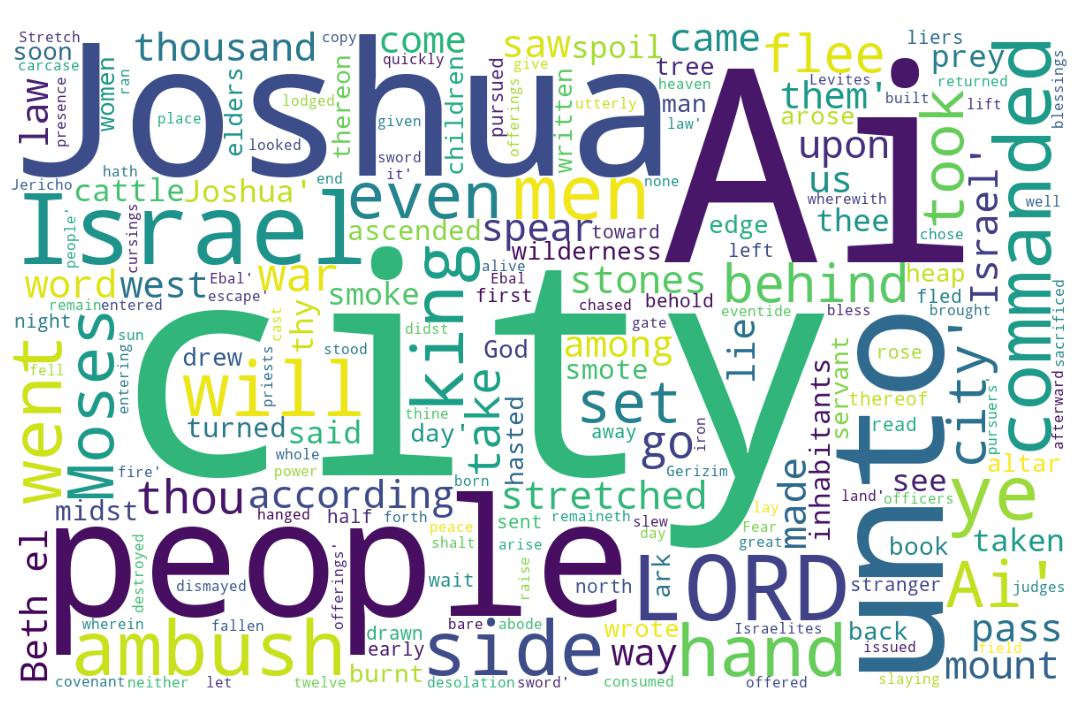
\includegraphics[width=\linewidth]{06OT-Joshua/Joshua8-WordCloud.jpg}
  \caption{Joshua 8 Word Cloud}
  \label{fig:Joshua 8 Word Cloud}
\end{figure}

\marginpar{\scriptsize \centering \fcolorbox{bone}{lime}{\textbf{ACHIN FOR A BRUSIN'}}\\ (Joshua 8)

\begin{compactenum}[I.][8]

	\item A \textbf{Never-Ending Promise} \index[scripture]{Joshua!Jsh 08:01}  (Jsh 8:1) 
	\item \textbf{No Procrastination} \index[scripture]{Joshua!Jsh 08:03}  (Jsh 8:3) 
	\item A \textbf{Nifty Plan} \index[scripture]{Joshua!Jsh 08:07}  (Jsh 8:7) 
	\item An \textbf{Unwise Pursuit} \index[scripture]{Joshua!Jsh 08:16--17}  (Jsh 8:16--17) 
	\item The \textbf{Number who Perished} \index[scripture]{Joshua!Jsh 08:25}  (Jsh 8:25) 
	\item A \textbf{National Presence} \index[scripture]{Joshua!Jsh 08:32}  (Jsh 8:32) 
	\item A \textbf{Notable Publication} \index[scripture]{Joshua!Jsh 08:34}  (Jsh 8:34) 
\end{compactenum}}


\footnote{\textcolor[cmyk]{0.99998,1,0,0}{\hyperlink{TOC}{Return to end of Table of Contents.}}}\textcolor[cmyk]{0.99998,1,0,0}{And the LORD said unto Joshua, Fear not, neither be thou dismayed: take all the \fcolorbox{bone}{bone}{people} of war with thee, and arise, go up to Ai: see, \fcolorbox{bone}{lime}{I have} \fcolorbox{bone}{lime}{given} into thy hand the king of Ai, and his \fcolorbox{bone}{bone}{people}, and his city, and his land:}
[2] \textcolor[cmyk]{0.99998,1,0,0}{And thou shalt do to Ai and her king as thou didst unto Jericho and her king: only the spoil thereof, and the cattle thereof, shall ye take for a prey unto yourselves: lay thee an ambush for the city behind it.}\\
\\
\P \textcolor[cmyk]{0.99998,1,0,0}{So Joshua arose, and all the \fcolorbox{bone}{bone}{people} of war, to go up against Ai: and Joshua chose out thirty thousand mighty men of valour, and \fcolorbox{bone}{lime}{sent them} \fcolorbox{bone}{lime}{away} by night.}
[4] \textcolor[cmyk]{0.99998,1,0,0}{And he commanded them, saying, Behold, ye shall lie in wa\fcolorbox{bone}{bone}{it} against the city, \emph{even} behind the city: go not very far from the city, but be ye all ready:}
[5] \textcolor[cmyk]{0.99998,1,0,0}{And I, and all the \fcolorbox{bone}{bone}{people} that \emph{are} with me, will approach unto the city: and \fcolorbox{bone}{bone}{it} shall come to pass, when they come out against us, as at the first, that we will flee before them,}
[6] \textcolor[cmyk]{0.99998,1,0,0}{(For they will come out after us) till we have drawn them from the city; for they will say, They flee before us, as at the first: therefore we will flee before them.}
[7] \textcolor[cmyk]{0.99998,1,0,0}{Then ye shall rise up from the ambush, and seize upon the city: for the LORD your \fcolorbox{bone}{lime}{God will deliver} \fcolorbox{bone}{bone}{it} into your hand.}
[8] \textcolor[cmyk]{0.99998,1,0,0}{And \fcolorbox{bone}{bone}{it} shall be, when ye have taken the city, \emph{that} ye shall set the city \fcolorbox{bone}{bone}{on} fire: according to the commandment of the LORD shall ye do. See, I have commanded you.}\\
\\
\P \textcolor[cmyk]{0.99998,1,0,0}{Joshua therefore sent them forth: and they went to lie in ambush, and abode between Beth-el and Ai, \fcolorbox{bone}{bone}{on} the west side of Ai: but Joshua lodged that night among the \fcolorbox{bone}{bone}{people}.}
[10] \textcolor[cmyk]{0.99998,1,0,0}{And Joshua rose up early in the morning, and numbered the \fcolorbox{bone}{bone}{people}, and went up, he and the elders of Israel, before the \fcolorbox{bone}{bone}{people} to Ai.}
[11] \textcolor[cmyk]{0.99998,1,0,0}{And all the \fcolorbox{bone}{bone}{people}, \emph{even} \emph{the} \emph{people} of war that \emph{were} with him, went up, and drew nigh, and came before the city, and pitched \fcolorbox{bone}{bone}{on} the north side of Ai: now \emph{there} \emph{was} a valley between them and Ai.}
[12] \textcolor[cmyk]{0.99998,1,0,0}{And he took about five thousand men, and set them to lie in ambush between Beth-el and Ai, \fcolorbox{bone}{bone}{on} the west side of the city.}
[13] \textcolor[cmyk]{0.99998,1,0,0}{And when they had set the \fcolorbox{bone}{bone}{people}, \emph{even} all the host that \emph{was} \fcolorbox{bone}{bone}{on} the north of the city, and their liers in wa\fcolorbox{bone}{bone}{it} \fcolorbox{bone}{bone}{on} the west of the city, Joshua went that night into the midst of the valley.}\\
\\
\P \textcolor[cmyk]{0.99998,1,0,0}{And \fcolorbox{bone}{bone}{it} came to pass, when the king of Ai saw \emph{it}, that they hasted and rose up early, and the men of the city went out against Israel to battle, he and all his \fcolorbox{bone}{bone}{people}, at a time appointed, before the plain; but he wist not that \emph{there} \emph{were} liers in ambush against him behind the city.}
[15] \textcolor[cmyk]{0.99998,1,0,0}{And Joshua and all Israel made as if they were beaten before them, and fled by the way of the wilderness.}
[16] \textcolor[cmyk]{0.99998,1,0,0}{And all the \fcolorbox{bone}{bone}{people} that \emph{were} in Ai were called together to \fcolorbox{bone}{lime}{pursue} after them: and they pursued after Joshua, and were drawn away from the city.}
[17] \textcolor[cmyk]{0.99998,1,0,0}{And there was not a man left in Ai or Beth-el, that went not out after Israel: and they left the city open, and pursued after Israel.}
[18] \textcolor[cmyk]{0.99998,1,0,0}{And the LORD said unto Joshua, Stretch out the spear that \emph{is} in thy hand toward Ai; for I will give \fcolorbox{bone}{bone}{it} into thine hand. And Joshua stretched out the spear that \emph{he} \emph{had} in his hand toward the city.}
[19] \textcolor[cmyk]{0.99998,1,0,0}{And the ambush arose quickly out of their place, and they ran as soon as he had stretched out his hand: and they entered into the city, and took it, and hasted and set the city \fcolorbox{bone}{bone}{on} fire.}
[20] \textcolor[cmyk]{0.99998,1,0,0}{And when the men of Ai looked behind them, they saw, and, behold, the smoke of the city ascended up to heaven, and they had no power to flee this way or that way: and the \fcolorbox{bone}{bone}{people} that fled to the wilderness turned back upon the pursuers.}
[21] \textcolor[cmyk]{0.99998,1,0,0}{And when Joshua and all Israel saw that the ambush had taken the city, and that the smoke of the city ascended, then they turned again, and slew the men of Ai.}
[22] \textcolor[cmyk]{0.99998,1,0,0}{And the other issued out of the city against them; so they were in the midst of Israel, some \fcolorbox{bone}{bone}{on} this side, and some \fcolorbox{bone}{bone}{on} that side: and they smote them, so that they let none of them remain or escape.}
[23] \textcolor[cmyk]{0.99998,1,0,0}{And the king of Ai they took alive, and brought him to Joshua.}
[24] \textcolor[cmyk]{0.99998,1,0,0}{And \fcolorbox{bone}{bone}{it} came to pass, when Israel had made an end of slaying all the inhabitants of Ai in the field, in the wilderness wherein they chased them, and when they were all fallen \fcolorbox{bone}{bone}{on} the edge of the sword, until they were consumed, that all the Israelites returned unto Ai, and smote \fcolorbox{bone}{bone}{it} with the edge of the sword.}
[25] \textcolor[cmyk]{0.99998,1,0,0}{And \emph{so} \fcolorbox{bone}{bone}{it} was, \emph{that} all that fell that day, both of men and women, \emph{were} \fcolorbox{bone}{lime}{twelve thousand}, \emph{even} all the men of Ai.}
[26] \textcolor[cmyk]{0.99998,1,0,0}{For Joshua drew not his hand back, wherewith he stretched out the spear, until he had utterly destroyed all the inhabitants of Ai.}
[27] \textcolor[cmyk]{0.99998,1,0,0}{Only the cattle and the spoil of that city Israel took for a prey unto themselves, according unto the word of the LORD which he commanded Joshua.}
[28] \textcolor[cmyk]{0.99998,1,0,0}{And Joshua burnt Ai, and made \fcolorbox{bone}{bone}{it} an heap for ever, \emph{even} a desolation unto this day.}
[29] \textcolor[cmyk]{0.99998,1,0,0}{And the king of Ai he hanged \fcolorbox{bone}{bone}{on} a tree until eventide: and as soon as the sun was down, Joshua commanded that they should take his carcase down from the tree, and cast \fcolorbox{bone}{bone}{it} at the entering of the gate of the city, and raise thereon a great heap of stones, \emph{that} \emph{remaineth} unto this day.}\\
\\
\P  \textcolor[cmyk]{0.99998,1,0,0}{Then Joshua built an altar unto the LORD God of Israel in mount Ebal,}
[31] \textcolor[cmyk]{0.99998,1,0,0}{As Moses the servant of the LORD commanded the children of Israel, as \fcolorbox{bone}{bone}{it} is written in the book of the law of Moses, an altar of whole stones, over which no man hath lift up \emph{any} iron: and they offered thereon burnt offerings unto the LORD, and sacrificed peace offerings.}\\
\\
\P \textcolor[cmyk]{0.99998,1,0,0}{And he wrote there upon the stones a copy of the law of Moses, which he wrote in the \fcolorbox{bone}{lime}{presence} of the children of Israel.}
[33] \textcolor[cmyk]{0.99998,1,0,0}{And all Israel, and their elders, and officers, and their judges, stood \fcolorbox{bone}{bone}{on} this side the ark and \fcolorbox{bone}{bone}{on} that side before the priests the Levites, which bare the ark of the covenant of the LORD, as well the stranger, as he that was born among them; half of them over against mount Gerizim, and half of them over against mount Ebal; as Moses the servant of the LORD had commanded before, that they should bless the \fcolorbox{bone}{bone}{people} of Israel.}
[34] \textcolor[cmyk]{0.99998,1,0,0}{And afterward \fcolorbox{bone}{lime}{he read} all the words of the law, the blessings and cursings, according to all that is written in the book of the law.}
[35] \textcolor[cmyk]{0.99998,1,0,0}{There was not a word of all that Moses commanded, which Joshua read not before all the congregation of Israel, with the women, and the little ones, and the strangers that were conversant among them.}


\index[NWIV]{46!Joshua!Jos 8:1}\index[AWIP]{And!Joshua!Jos 8:1}\index[AWIP]{the!Joshua!Jos 8:1}\index[AWIP]{the!Joshua!Jos 8:1 (2)}\index[AWIP]{the!Joshua!Jos 8:1 (3)}\index[AWIP]{LORD!Joshua!Jos 8:1}\index[AWIP]{said!Joshua!Jos 8:1}\index[AWIP]{unto!Joshua!Jos 8:1}\index[AWIP]{Joshua!Joshua!Jos 8:1}\index[AWIP]{Fear!Joshua!Jos 8:1}\index[AWIP]{not!Joshua!Jos 8:1}\index[AWIP]{neither!Joshua!Jos 8:1}\index[AWIP]{be!Joshua!Jos 8:1}\index[AWIP]{thou!Joshua!Jos 8:1}\index[AWIP]{dismayed!Joshua!Jos 8:1}\index[AWIP]{take!Joshua!Jos 8:1}\index[AWIP]{all!Joshua!Jos 8:1}\index[AWIP]{people!Joshua!Jos 8:1}\index[AWIP]{people!Joshua!Jos 8:1 (2)}\index[AWIP]{of!Joshua!Jos 8:1}\index[AWIP]{of!Joshua!Jos 8:1 (2)}\index[AWIP]{war!Joshua!Jos 8:1}\index[AWIP]{with!Joshua!Jos 8:1}\index[AWIP]{thee!Joshua!Jos 8:1}\index[AWIP]{and!Joshua!Jos 8:1}\index[AWIP]{and!Joshua!Jos 8:1 (2)}\index[AWIP]{and!Joshua!Jos 8:1 (3)}\index[AWIP]{and!Joshua!Jos 8:1 (4)}\index[AWIP]{arise!Joshua!Jos 8:1}\index[AWIP]{go!Joshua!Jos 8:1}\index[AWIP]{up!Joshua!Jos 8:1}\index[AWIP]{to!Joshua!Jos 8:1}\index[AWIP]{Ai!Joshua!Jos 8:1}\index[AWIP]{Ai!Joshua!Jos 8:1 (2)}\index[AWIP]{see!Joshua!Jos 8:1}\index[AWIP]{I!Joshua!Jos 8:1}\index[AWIP]{have!Joshua!Jos 8:1}\index[AWIP]{given!Joshua!Jos 8:1}\index[AWIP]{into!Joshua!Jos 8:1}\index[AWIP]{thy!Joshua!Jos 8:1}\index[AWIP]{hand!Joshua!Jos 8:1}\index[AWIP]{king!Joshua!Jos 8:1}\index[AWIP]{his!Joshua!Jos 8:1}\index[AWIP]{his!Joshua!Jos 8:1 (2)}\index[AWIP]{his!Joshua!Jos 8:1 (3)}\index[AWIP]{city!Joshua!Jos 8:1}\index[AWIP]{land!Joshua!Jos 8:1}

\index[NWIV]{42!Joshua!Jos 8:2}\index[AWIP]{And!Joshua!Jos 8:2}\index[AWIP]{thou!Joshua!Jos 8:2}\index[AWIP]{thou!Joshua!Jos 8:2 (2)}\index[AWIP]{shalt!Joshua!Jos 8:2}\index[AWIP]{do!Joshua!Jos 8:2}\index[AWIP]{to!Joshua!Jos 8:2}\index[AWIP]{Ai!Joshua!Jos 8:2}\index[AWIP]{and!Joshua!Jos 8:2}\index[AWIP]{and!Joshua!Jos 8:2 (2)}\index[AWIP]{and!Joshua!Jos 8:2 (3)}\index[AWIP]{her!Joshua!Jos 8:2}\index[AWIP]{her!Joshua!Jos 8:2 (2)}\index[AWIP]{king!Joshua!Jos 8:2}\index[AWIP]{king!Joshua!Jos 8:2 (2)}\index[AWIP]{as!Joshua!Jos 8:2}\index[AWIP]{didst!Joshua!Jos 8:2}\index[AWIP]{unto!Joshua!Jos 8:2}\index[AWIP]{unto!Joshua!Jos 8:2 (2)}\index[AWIP]{Jericho!Joshua!Jos 8:2}\index[AWIP]{only!Joshua!Jos 8:2}\index[AWIP]{the!Joshua!Jos 8:2}\index[AWIP]{the!Joshua!Jos 8:2 (2)}\index[AWIP]{the!Joshua!Jos 8:2 (3)}\index[AWIP]{spoil!Joshua!Jos 8:2}\index[AWIP]{thereof!Joshua!Jos 8:2}\index[AWIP]{thereof!Joshua!Jos 8:2 (2)}\index[AWIP]{cattle!Joshua!Jos 8:2}\index[AWIP]{shall!Joshua!Jos 8:2}\index[AWIP]{ye!Joshua!Jos 8:2}\index[AWIP]{take!Joshua!Jos 8:2}\index[AWIP]{for!Joshua!Jos 8:2}\index[AWIP]{for!Joshua!Jos 8:2 (2)}\index[AWIP]{a!Joshua!Jos 8:2}\index[AWIP]{prey!Joshua!Jos 8:2}\index[AWIP]{yourselves!Joshua!Jos 8:2}\index[AWIP]{lay!Joshua!Jos 8:2}\index[AWIP]{thee!Joshua!Jos 8:2}\index[AWIP]{an!Joshua!Jos 8:2}\index[AWIP]{ambush!Joshua!Jos 8:2}\index[AWIP]{city!Joshua!Jos 8:2}\index[AWIP]{behind!Joshua!Jos 8:2}\index[AWIP]{it!Joshua!Jos 8:2}

\index[NWIV]{30!Joshua!Jos 8:3}\index[AWIP]{So!Joshua!Jos 8:3}\index[AWIP]{Joshua!Joshua!Jos 8:3}\index[AWIP]{Joshua!Joshua!Jos 8:3 (2)}\index[AWIP]{arose!Joshua!Jos 8:3}\index[AWIP]{and!Joshua!Jos 8:3}\index[AWIP]{and!Joshua!Jos 8:3 (2)}\index[AWIP]{and!Joshua!Jos 8:3 (3)}\index[AWIP]{all!Joshua!Jos 8:3}\index[AWIP]{the!Joshua!Jos 8:3}\index[AWIP]{people!Joshua!Jos 8:3}\index[AWIP]{of!Joshua!Jos 8:3}\index[AWIP]{of!Joshua!Jos 8:3 (2)}\index[AWIP]{war!Joshua!Jos 8:3}\index[AWIP]{to!Joshua!Jos 8:3}\index[AWIP]{go!Joshua!Jos 8:3}\index[AWIP]{up!Joshua!Jos 8:3}\index[AWIP]{against!Joshua!Jos 8:3}\index[AWIP]{Ai!Joshua!Jos 8:3}\index[AWIP]{chose!Joshua!Jos 8:3}\index[AWIP]{out!Joshua!Jos 8:3}\index[AWIP]{thirty!Joshua!Jos 8:3}\index[AWIP]{thousand!Joshua!Jos 8:3}\index[AWIP]{mighty!Joshua!Jos 8:3}\index[AWIP]{men!Joshua!Jos 8:3}\index[AWIP]{valour!Joshua!Jos 8:3}\index[AWIP]{sent!Joshua!Jos 8:3}\index[AWIP]{them!Joshua!Jos 8:3}\index[AWIP]{away!Joshua!Jos 8:3}\index[AWIP]{by!Joshua!Jos 8:3}\index[AWIP]{night!Joshua!Jos 8:3}

\index[NWIV]{30!Joshua!Jos 8:4}\index[AWIP]{And!Joshua!Jos 8:4}\index[AWIP]{he!Joshua!Jos 8:4}\index[AWIP]{commanded!Joshua!Jos 8:4}\index[AWIP]{them!Joshua!Jos 8:4}\index[AWIP]{saying!Joshua!Jos 8:4}\index[AWIP]{Behold!Joshua!Jos 8:4}\index[AWIP]{ye!Joshua!Jos 8:4}\index[AWIP]{ye!Joshua!Jos 8:4 (2)}\index[AWIP]{shall!Joshua!Jos 8:4}\index[AWIP]{lie!Joshua!Jos 8:4}\index[AWIP]{in!Joshua!Jos 8:4}\index[AWIP]{wait!Joshua!Jos 8:4}\index[AWIP]{against!Joshua!Jos 8:4}\index[AWIP]{the!Joshua!Jos 8:4}\index[AWIP]{the!Joshua!Jos 8:4 (2)}\index[AWIP]{the!Joshua!Jos 8:4 (3)}\index[AWIP]{city!Joshua!Jos 8:4}\index[AWIP]{city!Joshua!Jos 8:4 (2)}\index[AWIP]{city!Joshua!Jos 8:4 (3)}\index[AWIP]{\emph{even}!Joshua!Jos 8:4}\index[AWIP]{behind!Joshua!Jos 8:4}\index[AWIP]{go!Joshua!Jos 8:4}\index[AWIP]{not!Joshua!Jos 8:4}\index[AWIP]{very!Joshua!Jos 8:4}\index[AWIP]{far!Joshua!Jos 8:4}\index[AWIP]{from!Joshua!Jos 8:4}\index[AWIP]{but!Joshua!Jos 8:4}\index[AWIP]{be!Joshua!Jos 8:4}\index[AWIP]{all!Joshua!Jos 8:4}\index[AWIP]{ready!Joshua!Jos 8:4}\index[AWIP]{\emph{even}!Joshua!Jos 8:4}

\index[NWIV]{37!Joshua!Jos 8:5}\index[AWIP]{And!Joshua!Jos 8:5}\index[AWIP]{I!Joshua!Jos 8:5}\index[AWIP]{and!Joshua!Jos 8:5}\index[AWIP]{and!Joshua!Jos 8:5 (2)}\index[AWIP]{all!Joshua!Jos 8:5}\index[AWIP]{the!Joshua!Jos 8:5}\index[AWIP]{the!Joshua!Jos 8:5 (2)}\index[AWIP]{the!Joshua!Jos 8:5 (3)}\index[AWIP]{people!Joshua!Jos 8:5}\index[AWIP]{that!Joshua!Jos 8:5}\index[AWIP]{that!Joshua!Jos 8:5 (2)}\index[AWIP]{\emph{are}!Joshua!Jos 8:5}\index[AWIP]{with!Joshua!Jos 8:5}\index[AWIP]{me!Joshua!Jos 8:5}\index[AWIP]{will!Joshua!Jos 8:5}\index[AWIP]{will!Joshua!Jos 8:5 (2)}\index[AWIP]{approach!Joshua!Jos 8:5}\index[AWIP]{unto!Joshua!Jos 8:5}\index[AWIP]{city!Joshua!Jos 8:5}\index[AWIP]{it!Joshua!Jos 8:5}\index[AWIP]{shall!Joshua!Jos 8:5}\index[AWIP]{come!Joshua!Jos 8:5}\index[AWIP]{come!Joshua!Jos 8:5 (2)}\index[AWIP]{to!Joshua!Jos 8:5}\index[AWIP]{pass!Joshua!Jos 8:5}\index[AWIP]{when!Joshua!Jos 8:5}\index[AWIP]{they!Joshua!Jos 8:5}\index[AWIP]{out!Joshua!Jos 8:5}\index[AWIP]{against!Joshua!Jos 8:5}\index[AWIP]{us!Joshua!Jos 8:5}\index[AWIP]{as!Joshua!Jos 8:5}\index[AWIP]{at!Joshua!Jos 8:5}\index[AWIP]{first!Joshua!Jos 8:5}\index[AWIP]{we!Joshua!Jos 8:5}\index[AWIP]{flee!Joshua!Jos 8:5}\index[AWIP]{before!Joshua!Jos 8:5}\index[AWIP]{them!Joshua!Jos 8:5}\index[AWIP]{\emph{are}!Joshua!Jos 8:5}

\index[NWIV]{33!Joshua!Jos 8:6}\index[AWIP]{(For!Joshua!Jos 8:6}\index[AWIP]{they!Joshua!Jos 8:6}\index[AWIP]{they!Joshua!Jos 8:6 (2)}\index[AWIP]{will!Joshua!Jos 8:6}\index[AWIP]{will!Joshua!Jos 8:6 (2)}\index[AWIP]{will!Joshua!Jos 8:6 (3)}\index[AWIP]{come!Joshua!Jos 8:6}\index[AWIP]{out!Joshua!Jos 8:6}\index[AWIP]{after!Joshua!Jos 8:6}\index[AWIP]{us)!Joshua!Jos 8:6}\index[AWIP]{till!Joshua!Jos 8:6}\index[AWIP]{we!Joshua!Jos 8:6}\index[AWIP]{we!Joshua!Jos 8:6 (2)}\index[AWIP]{have!Joshua!Jos 8:6}\index[AWIP]{drawn!Joshua!Jos 8:6}\index[AWIP]{them!Joshua!Jos 8:6}\index[AWIP]{them!Joshua!Jos 8:6 (2)}\index[AWIP]{from!Joshua!Jos 8:6}\index[AWIP]{the!Joshua!Jos 8:6}\index[AWIP]{the!Joshua!Jos 8:6 (2)}\index[AWIP]{city!Joshua!Jos 8:6}\index[AWIP]{for!Joshua!Jos 8:6}\index[AWIP]{say!Joshua!Jos 8:6}\index[AWIP]{They!Joshua!Jos 8:6}\index[AWIP]{flee!Joshua!Jos 8:6}\index[AWIP]{flee!Joshua!Jos 8:6 (2)}\index[AWIP]{before!Joshua!Jos 8:6}\index[AWIP]{before!Joshua!Jos 8:6 (2)}\index[AWIP]{us!Joshua!Jos 8:6}\index[AWIP]{as!Joshua!Jos 8:6}\index[AWIP]{at!Joshua!Jos 8:6}\index[AWIP]{first!Joshua!Jos 8:6}\index[AWIP]{therefore!Joshua!Jos 8:6}

\index[NWIV]{24!Joshua!Jos 8:7}\index[AWIP]{Then!Joshua!Jos 8:7}\index[AWIP]{ye!Joshua!Jos 8:7}\index[AWIP]{shall!Joshua!Jos 8:7}\index[AWIP]{rise!Joshua!Jos 8:7}\index[AWIP]{up!Joshua!Jos 8:7}\index[AWIP]{from!Joshua!Jos 8:7}\index[AWIP]{the!Joshua!Jos 8:7}\index[AWIP]{the!Joshua!Jos 8:7 (2)}\index[AWIP]{the!Joshua!Jos 8:7 (3)}\index[AWIP]{ambush!Joshua!Jos 8:7}\index[AWIP]{and!Joshua!Jos 8:7}\index[AWIP]{seize!Joshua!Jos 8:7}\index[AWIP]{upon!Joshua!Jos 8:7}\index[AWIP]{city!Joshua!Jos 8:7}\index[AWIP]{for!Joshua!Jos 8:7}\index[AWIP]{LORD!Joshua!Jos 8:7}\index[AWIP]{your!Joshua!Jos 8:7}\index[AWIP]{your!Joshua!Jos 8:7 (2)}\index[AWIP]{God!Joshua!Jos 8:7}\index[AWIP]{will!Joshua!Jos 8:7}\index[AWIP]{deliver!Joshua!Jos 8:7}\index[AWIP]{it!Joshua!Jos 8:7}\index[AWIP]{into!Joshua!Jos 8:7}\index[AWIP]{hand!Joshua!Jos 8:7}

\index[NWIV]{33!Joshua!Jos 8:8}\index[AWIP]{And!Joshua!Jos 8:8}\index[AWIP]{it!Joshua!Jos 8:8}\index[AWIP]{shall!Joshua!Jos 8:8}\index[AWIP]{shall!Joshua!Jos 8:8 (2)}\index[AWIP]{shall!Joshua!Jos 8:8 (3)}\index[AWIP]{be!Joshua!Jos 8:8}\index[AWIP]{when!Joshua!Jos 8:8}\index[AWIP]{ye!Joshua!Jos 8:8}\index[AWIP]{ye!Joshua!Jos 8:8 (2)}\index[AWIP]{ye!Joshua!Jos 8:8 (3)}\index[AWIP]{have!Joshua!Jos 8:8}\index[AWIP]{have!Joshua!Jos 8:8 (2)}\index[AWIP]{taken!Joshua!Jos 8:8}\index[AWIP]{the!Joshua!Jos 8:8}\index[AWIP]{the!Joshua!Jos 8:8 (2)}\index[AWIP]{the!Joshua!Jos 8:8 (3)}\index[AWIP]{the!Joshua!Jos 8:8 (4)}\index[AWIP]{city!Joshua!Jos 8:8}\index[AWIP]{city!Joshua!Jos 8:8 (2)}\index[AWIP]{\emph{that}!Joshua!Jos 8:8}\index[AWIP]{set!Joshua!Jos 8:8}\index[AWIP]{on!Joshua!Jos 8:8}\index[AWIP]{fire!Joshua!Jos 8:8}\index[AWIP]{according!Joshua!Jos 8:8}\index[AWIP]{to!Joshua!Jos 8:8}\index[AWIP]{commandment!Joshua!Jos 8:8}\index[AWIP]{of!Joshua!Jos 8:8}\index[AWIP]{LORD!Joshua!Jos 8:8}\index[AWIP]{do!Joshua!Jos 8:8}\index[AWIP]{See!Joshua!Jos 8:8}\index[AWIP]{I!Joshua!Jos 8:8}\index[AWIP]{commanded!Joshua!Jos 8:8}\index[AWIP]{you!Joshua!Jos 8:8}\index[AWIP]{\emph{that}!Joshua!Jos 8:8}

\index[NWIV]{32!Joshua!Jos 8:9}\index[AWIP]{Joshua!Joshua!Jos 8:9}\index[AWIP]{Joshua!Joshua!Jos 8:9 (2)}\index[AWIP]{therefore!Joshua!Jos 8:9}\index[AWIP]{sent!Joshua!Jos 8:9}\index[AWIP]{them!Joshua!Jos 8:9}\index[AWIP]{forth!Joshua!Jos 8:9}\index[AWIP]{and!Joshua!Jos 8:9}\index[AWIP]{and!Joshua!Jos 8:9 (2)}\index[AWIP]{and!Joshua!Jos 8:9 (3)}\index[AWIP]{they!Joshua!Jos 8:9}\index[AWIP]{went!Joshua!Jos 8:9}\index[AWIP]{to!Joshua!Jos 8:9}\index[AWIP]{lie!Joshua!Jos 8:9}\index[AWIP]{in!Joshua!Jos 8:9}\index[AWIP]{ambush!Joshua!Jos 8:9}\index[AWIP]{abode!Joshua!Jos 8:9}\index[AWIP]{between!Joshua!Jos 8:9}\index[AWIP]{Beth-el!Joshua!Jos 8:9}\index[AWIP]{Ai!Joshua!Jos 8:9}\index[AWIP]{Ai!Joshua!Jos 8:9 (2)}\index[AWIP]{on!Joshua!Jos 8:9}\index[AWIP]{the!Joshua!Jos 8:9}\index[AWIP]{the!Joshua!Jos 8:9 (2)}\index[AWIP]{west!Joshua!Jos 8:9}\index[AWIP]{side!Joshua!Jos 8:9}\index[AWIP]{of!Joshua!Jos 8:9}\index[AWIP]{but!Joshua!Jos 8:9}\index[AWIP]{lodged!Joshua!Jos 8:9}\index[AWIP]{that!Joshua!Jos 8:9}\index[AWIP]{night!Joshua!Jos 8:9}\index[AWIP]{among!Joshua!Jos 8:9}\index[AWIP]{people!Joshua!Jos 8:9}

\index[NWIV]{26!Joshua!Jos 8:10}\index[AWIP]{And!Joshua!Jos 8:10}\index[AWIP]{Joshua!Joshua!Jos 8:10}\index[AWIP]{rose!Joshua!Jos 8:10}\index[AWIP]{up!Joshua!Jos 8:10}\index[AWIP]{up!Joshua!Jos 8:10 (2)}\index[AWIP]{early!Joshua!Jos 8:10}\index[AWIP]{in!Joshua!Jos 8:10}\index[AWIP]{the!Joshua!Jos 8:10}\index[AWIP]{the!Joshua!Jos 8:10 (2)}\index[AWIP]{the!Joshua!Jos 8:10 (3)}\index[AWIP]{the!Joshua!Jos 8:10 (4)}\index[AWIP]{morning!Joshua!Jos 8:10}\index[AWIP]{and!Joshua!Jos 8:10}\index[AWIP]{and!Joshua!Jos 8:10 (2)}\index[AWIP]{and!Joshua!Jos 8:10 (3)}\index[AWIP]{numbered!Joshua!Jos 8:10}\index[AWIP]{people!Joshua!Jos 8:10}\index[AWIP]{people!Joshua!Jos 8:10 (2)}\index[AWIP]{went!Joshua!Jos 8:10}\index[AWIP]{he!Joshua!Jos 8:10}\index[AWIP]{elders!Joshua!Jos 8:10}\index[AWIP]{of!Joshua!Jos 8:10}\index[AWIP]{Israel!Joshua!Jos 8:10}\index[AWIP]{before!Joshua!Jos 8:10}\index[AWIP]{to!Joshua!Jos 8:10}\index[AWIP]{Ai!Joshua!Jos 8:10}

\index[NWIV]{40!Joshua!Jos 8:11}\index[AWIP]{And!Joshua!Jos 8:11}\index[AWIP]{all!Joshua!Jos 8:11}\index[AWIP]{the!Joshua!Jos 8:11}\index[AWIP]{the!Joshua!Jos 8:11 (2)}\index[AWIP]{the!Joshua!Jos 8:11 (3)}\index[AWIP]{people!Joshua!Jos 8:11}\index[AWIP]{\emph{even}!Joshua!Jos 8:11}\index[AWIP]{\emph{the}!Joshua!Jos 8:11}\index[AWIP]{\emph{people}!Joshua!Jos 8:11}\index[AWIP]{of!Joshua!Jos 8:11}\index[AWIP]{of!Joshua!Jos 8:11 (2)}\index[AWIP]{war!Joshua!Jos 8:11}\index[AWIP]{that!Joshua!Jos 8:11}\index[AWIP]{\emph{were}!Joshua!Jos 8:11}\index[AWIP]{with!Joshua!Jos 8:11}\index[AWIP]{him!Joshua!Jos 8:11}\index[AWIP]{went!Joshua!Jos 8:11}\index[AWIP]{up!Joshua!Jos 8:11}\index[AWIP]{and!Joshua!Jos 8:11}\index[AWIP]{and!Joshua!Jos 8:11 (2)}\index[AWIP]{and!Joshua!Jos 8:11 (3)}\index[AWIP]{and!Joshua!Jos 8:11 (4)}\index[AWIP]{drew!Joshua!Jos 8:11}\index[AWIP]{nigh!Joshua!Jos 8:11}\index[AWIP]{came!Joshua!Jos 8:11}\index[AWIP]{before!Joshua!Jos 8:11}\index[AWIP]{city!Joshua!Jos 8:11}\index[AWIP]{pitched!Joshua!Jos 8:11}\index[AWIP]{on!Joshua!Jos 8:11}\index[AWIP]{north!Joshua!Jos 8:11}\index[AWIP]{side!Joshua!Jos 8:11}\index[AWIP]{Ai!Joshua!Jos 8:11}\index[AWIP]{Ai!Joshua!Jos 8:11 (2)}\index[AWIP]{now!Joshua!Jos 8:11}\index[AWIP]{\emph{there}!Joshua!Jos 8:11}\index[AWIP]{\emph{was}!Joshua!Jos 8:11}\index[AWIP]{a!Joshua!Jos 8:11}\index[AWIP]{valley!Joshua!Jos 8:11}\index[AWIP]{between!Joshua!Jos 8:11}\index[AWIP]{them!Joshua!Jos 8:11}\index[AWIP]{\emph{even}!Joshua!Jos 8:11}\index[AWIP]{\emph{the}!Joshua!Jos 8:11}\index[AWIP]{\emph{people}!Joshua!Jos 8:11}\index[AWIP]{\emph{were}!Joshua!Jos 8:11}\index[AWIP]{\emph{there}!Joshua!Jos 8:11}\index[AWIP]{\emph{was}!Joshua!Jos 8:11}

\index[NWIV]{25!Joshua!Jos 8:12}\index[AWIP]{And!Joshua!Jos 8:12}\index[AWIP]{he!Joshua!Jos 8:12}\index[AWIP]{took!Joshua!Jos 8:12}\index[AWIP]{about!Joshua!Jos 8:12}\index[AWIP]{five!Joshua!Jos 8:12}\index[AWIP]{thousand!Joshua!Jos 8:12}\index[AWIP]{men!Joshua!Jos 8:12}\index[AWIP]{and!Joshua!Jos 8:12}\index[AWIP]{and!Joshua!Jos 8:12 (2)}\index[AWIP]{set!Joshua!Jos 8:12}\index[AWIP]{them!Joshua!Jos 8:12}\index[AWIP]{to!Joshua!Jos 8:12}\index[AWIP]{lie!Joshua!Jos 8:12}\index[AWIP]{in!Joshua!Jos 8:12}\index[AWIP]{ambush!Joshua!Jos 8:12}\index[AWIP]{between!Joshua!Jos 8:12}\index[AWIP]{Beth-el!Joshua!Jos 8:12}\index[AWIP]{Ai!Joshua!Jos 8:12}\index[AWIP]{on!Joshua!Jos 8:12}\index[AWIP]{the!Joshua!Jos 8:12}\index[AWIP]{the!Joshua!Jos 8:12 (2)}\index[AWIP]{west!Joshua!Jos 8:12}\index[AWIP]{side!Joshua!Jos 8:12}\index[AWIP]{of!Joshua!Jos 8:12}\index[AWIP]{city!Joshua!Jos 8:12}

\index[NWIV]{40!Joshua!Jos 8:13}\index[AWIP]{And!Joshua!Jos 8:13}\index[AWIP]{when!Joshua!Jos 8:13}\index[AWIP]{they!Joshua!Jos 8:13}\index[AWIP]{had!Joshua!Jos 8:13}\index[AWIP]{set!Joshua!Jos 8:13}\index[AWIP]{the!Joshua!Jos 8:13}\index[AWIP]{the!Joshua!Jos 8:13 (2)}\index[AWIP]{the!Joshua!Jos 8:13 (3)}\index[AWIP]{the!Joshua!Jos 8:13 (4)}\index[AWIP]{the!Joshua!Jos 8:13 (5)}\index[AWIP]{the!Joshua!Jos 8:13 (6)}\index[AWIP]{the!Joshua!Jos 8:13 (7)}\index[AWIP]{the!Joshua!Jos 8:13 (8)}\index[AWIP]{people!Joshua!Jos 8:13}\index[AWIP]{\emph{even}!Joshua!Jos 8:13}\index[AWIP]{all!Joshua!Jos 8:13}\index[AWIP]{host!Joshua!Jos 8:13}\index[AWIP]{that!Joshua!Jos 8:13}\index[AWIP]{that!Joshua!Jos 8:13 (2)}\index[AWIP]{\emph{was}!Joshua!Jos 8:13}\index[AWIP]{on!Joshua!Jos 8:13}\index[AWIP]{on!Joshua!Jos 8:13 (2)}\index[AWIP]{north!Joshua!Jos 8:13}\index[AWIP]{of!Joshua!Jos 8:13}\index[AWIP]{of!Joshua!Jos 8:13 (2)}\index[AWIP]{of!Joshua!Jos 8:13 (3)}\index[AWIP]{city!Joshua!Jos 8:13}\index[AWIP]{city!Joshua!Jos 8:13 (2)}\index[AWIP]{and!Joshua!Jos 8:13}\index[AWIP]{their!Joshua!Jos 8:13}\index[AWIP]{liers!Joshua!Jos 8:13}\index[AWIP]{in!Joshua!Jos 8:13}\index[AWIP]{wait!Joshua!Jos 8:13}\index[AWIP]{west!Joshua!Jos 8:13}\index[AWIP]{Joshua!Joshua!Jos 8:13}\index[AWIP]{went!Joshua!Jos 8:13}\index[AWIP]{night!Joshua!Jos 8:13}\index[AWIP]{into!Joshua!Jos 8:13}\index[AWIP]{midst!Joshua!Jos 8:13}\index[AWIP]{valley!Joshua!Jos 8:13}\index[AWIP]{\emph{even}!Joshua!Jos 8:13}\index[AWIP]{\emph{was}!Joshua!Jos 8:13}

\index[NWIV]{58!Joshua!Jos 8:14}\index[AWIP]{And!Joshua!Jos 8:14}\index[AWIP]{it!Joshua!Jos 8:14}\index[AWIP]{came!Joshua!Jos 8:14}\index[AWIP]{to!Joshua!Jos 8:14}\index[AWIP]{to!Joshua!Jos 8:14 (2)}\index[AWIP]{pass!Joshua!Jos 8:14}\index[AWIP]{when!Joshua!Jos 8:14}\index[AWIP]{the!Joshua!Jos 8:14}\index[AWIP]{the!Joshua!Jos 8:14 (2)}\index[AWIP]{the!Joshua!Jos 8:14 (3)}\index[AWIP]{the!Joshua!Jos 8:14 (4)}\index[AWIP]{the!Joshua!Jos 8:14 (5)}\index[AWIP]{king!Joshua!Jos 8:14}\index[AWIP]{of!Joshua!Jos 8:14}\index[AWIP]{of!Joshua!Jos 8:14 (2)}\index[AWIP]{Ai!Joshua!Jos 8:14}\index[AWIP]{saw!Joshua!Jos 8:14}\index[AWIP]{\emph{it}!Joshua!Jos 8:14}\index[AWIP]{that!Joshua!Jos 8:14}\index[AWIP]{that!Joshua!Jos 8:14 (2)}\index[AWIP]{they!Joshua!Jos 8:14}\index[AWIP]{hasted!Joshua!Jos 8:14}\index[AWIP]{and!Joshua!Jos 8:14}\index[AWIP]{and!Joshua!Jos 8:14 (2)}\index[AWIP]{and!Joshua!Jos 8:14 (3)}\index[AWIP]{rose!Joshua!Jos 8:14}\index[AWIP]{up!Joshua!Jos 8:14}\index[AWIP]{early!Joshua!Jos 8:14}\index[AWIP]{men!Joshua!Jos 8:14}\index[AWIP]{city!Joshua!Jos 8:14}\index[AWIP]{city!Joshua!Jos 8:14 (2)}\index[AWIP]{went!Joshua!Jos 8:14}\index[AWIP]{out!Joshua!Jos 8:14}\index[AWIP]{against!Joshua!Jos 8:14}\index[AWIP]{against!Joshua!Jos 8:14 (2)}\index[AWIP]{Israel!Joshua!Jos 8:14}\index[AWIP]{battle!Joshua!Jos 8:14}\index[AWIP]{he!Joshua!Jos 8:14}\index[AWIP]{he!Joshua!Jos 8:14 (2)}\index[AWIP]{all!Joshua!Jos 8:14}\index[AWIP]{his!Joshua!Jos 8:14}\index[AWIP]{people!Joshua!Jos 8:14}\index[AWIP]{at!Joshua!Jos 8:14}\index[AWIP]{a!Joshua!Jos 8:14}\index[AWIP]{time!Joshua!Jos 8:14}\index[AWIP]{appointed!Joshua!Jos 8:14}\index[AWIP]{before!Joshua!Jos 8:14}\index[AWIP]{plain!Joshua!Jos 8:14}\index[AWIP]{but!Joshua!Jos 8:14}\index[AWIP]{wist!Joshua!Jos 8:14}\index[AWIP]{not!Joshua!Jos 8:14}\index[AWIP]{\emph{there}!Joshua!Jos 8:14}\index[AWIP]{\emph{were}!Joshua!Jos 8:14}\index[AWIP]{liers!Joshua!Jos 8:14}\index[AWIP]{in!Joshua!Jos 8:14}\index[AWIP]{ambush!Joshua!Jos 8:14}\index[AWIP]{him!Joshua!Jos 8:14}\index[AWIP]{behind!Joshua!Jos 8:14}\index[AWIP]{\emph{it}!Joshua!Jos 8:14}\index[AWIP]{\emph{there}!Joshua!Jos 8:14}\index[AWIP]{\emph{were}!Joshua!Jos 8:14}

\index[NWIV]{21!Joshua!Jos 8:15}\index[AWIP]{And!Joshua!Jos 8:15}\index[AWIP]{Joshua!Joshua!Jos 8:15}\index[AWIP]{and!Joshua!Jos 8:15}\index[AWIP]{and!Joshua!Jos 8:15 (2)}\index[AWIP]{all!Joshua!Jos 8:15}\index[AWIP]{Israel!Joshua!Jos 8:15}\index[AWIP]{made!Joshua!Jos 8:15}\index[AWIP]{as!Joshua!Jos 8:15}\index[AWIP]{if!Joshua!Jos 8:15}\index[AWIP]{they!Joshua!Jos 8:15}\index[AWIP]{were!Joshua!Jos 8:15}\index[AWIP]{beaten!Joshua!Jos 8:15}\index[AWIP]{before!Joshua!Jos 8:15}\index[AWIP]{them!Joshua!Jos 8:15}\index[AWIP]{fled!Joshua!Jos 8:15}\index[AWIP]{by!Joshua!Jos 8:15}\index[AWIP]{the!Joshua!Jos 8:15}\index[AWIP]{the!Joshua!Jos 8:15 (2)}\index[AWIP]{way!Joshua!Jos 8:15}\index[AWIP]{of!Joshua!Jos 8:15}\index[AWIP]{wilderness!Joshua!Jos 8:15}

\index[NWIV]{27!Joshua!Jos 8:16}\index[AWIP]{And!Joshua!Jos 8:16}\index[AWIP]{all!Joshua!Jos 8:16}\index[AWIP]{the!Joshua!Jos 8:16}\index[AWIP]{the!Joshua!Jos 8:16 (2)}\index[AWIP]{people!Joshua!Jos 8:16}\index[AWIP]{that!Joshua!Jos 8:16}\index[AWIP]{\emph{were}!Joshua!Jos 8:16}\index[AWIP]{in!Joshua!Jos 8:16}\index[AWIP]{Ai!Joshua!Jos 8:16}\index[AWIP]{were!Joshua!Jos 8:16}\index[AWIP]{were!Joshua!Jos 8:16 (2)}\index[AWIP]{called!Joshua!Jos 8:16}\index[AWIP]{together!Joshua!Jos 8:16}\index[AWIP]{to!Joshua!Jos 8:16}\index[AWIP]{pursue!Joshua!Jos 8:16}\index[AWIP]{after!Joshua!Jos 8:16}\index[AWIP]{after!Joshua!Jos 8:16 (2)}\index[AWIP]{them!Joshua!Jos 8:16}\index[AWIP]{and!Joshua!Jos 8:16}\index[AWIP]{and!Joshua!Jos 8:16 (2)}\index[AWIP]{they!Joshua!Jos 8:16}\index[AWIP]{pursued!Joshua!Jos 8:16}\index[AWIP]{Joshua!Joshua!Jos 8:16}\index[AWIP]{drawn!Joshua!Jos 8:16}\index[AWIP]{away!Joshua!Jos 8:16}\index[AWIP]{from!Joshua!Jos 8:16}\index[AWIP]{city!Joshua!Jos 8:16}\index[AWIP]{\emph{were}!Joshua!Jos 8:16}

\index[NWIV]{27!Joshua!Jos 8:17}\index[AWIP]{And!Joshua!Jos 8:17}\index[AWIP]{there!Joshua!Jos 8:17}\index[AWIP]{was!Joshua!Jos 8:17}\index[AWIP]{not!Joshua!Jos 8:17}\index[AWIP]{not!Joshua!Jos 8:17 (2)}\index[AWIP]{a!Joshua!Jos 8:17}\index[AWIP]{man!Joshua!Jos 8:17}\index[AWIP]{left!Joshua!Jos 8:17}\index[AWIP]{left!Joshua!Jos 8:17 (2)}\index[AWIP]{in!Joshua!Jos 8:17}\index[AWIP]{Ai!Joshua!Jos 8:17}\index[AWIP]{or!Joshua!Jos 8:17}\index[AWIP]{Beth-el!Joshua!Jos 8:17}\index[AWIP]{that!Joshua!Jos 8:17}\index[AWIP]{went!Joshua!Jos 8:17}\index[AWIP]{out!Joshua!Jos 8:17}\index[AWIP]{after!Joshua!Jos 8:17}\index[AWIP]{after!Joshua!Jos 8:17 (2)}\index[AWIP]{Israel!Joshua!Jos 8:17}\index[AWIP]{Israel!Joshua!Jos 8:17 (2)}\index[AWIP]{and!Joshua!Jos 8:17}\index[AWIP]{and!Joshua!Jos 8:17 (2)}\index[AWIP]{they!Joshua!Jos 8:17}\index[AWIP]{the!Joshua!Jos 8:17}\index[AWIP]{city!Joshua!Jos 8:17}\index[AWIP]{open!Joshua!Jos 8:17}\index[AWIP]{pursued!Joshua!Jos 8:17}

\index[NWIV]{40!Joshua!Jos 8:18}\index[AWIP]{And!Joshua!Jos 8:18}\index[AWIP]{And!Joshua!Jos 8:18 (2)}\index[AWIP]{the!Joshua!Jos 8:18}\index[AWIP]{the!Joshua!Jos 8:18 (2)}\index[AWIP]{the!Joshua!Jos 8:18 (3)}\index[AWIP]{the!Joshua!Jos 8:18 (4)}\index[AWIP]{LORD!Joshua!Jos 8:18}\index[AWIP]{said!Joshua!Jos 8:18}\index[AWIP]{unto!Joshua!Jos 8:18}\index[AWIP]{Joshua!Joshua!Jos 8:18}\index[AWIP]{Joshua!Joshua!Jos 8:18 (2)}\index[AWIP]{Stretch!Joshua!Jos 8:18}\index[AWIP]{out!Joshua!Jos 8:18}\index[AWIP]{out!Joshua!Jos 8:18 (2)}\index[AWIP]{spear!Joshua!Jos 8:18}\index[AWIP]{spear!Joshua!Jos 8:18 (2)}\index[AWIP]{that!Joshua!Jos 8:18}\index[AWIP]{that!Joshua!Jos 8:18 (2)}\index[AWIP]{\emph{is}!Joshua!Jos 8:18}\index[AWIP]{in!Joshua!Jos 8:18}\index[AWIP]{in!Joshua!Jos 8:18 (2)}\index[AWIP]{thy!Joshua!Jos 8:18}\index[AWIP]{hand!Joshua!Jos 8:18}\index[AWIP]{hand!Joshua!Jos 8:18 (2)}\index[AWIP]{hand!Joshua!Jos 8:18 (3)}\index[AWIP]{toward!Joshua!Jos 8:18}\index[AWIP]{toward!Joshua!Jos 8:18 (2)}\index[AWIP]{Ai!Joshua!Jos 8:18}\index[AWIP]{for!Joshua!Jos 8:18}\index[AWIP]{I!Joshua!Jos 8:18}\index[AWIP]{will!Joshua!Jos 8:18}\index[AWIP]{give!Joshua!Jos 8:18}\index[AWIP]{it!Joshua!Jos 8:18}\index[AWIP]{into!Joshua!Jos 8:18}\index[AWIP]{thine!Joshua!Jos 8:18}\index[AWIP]{stretched!Joshua!Jos 8:18}\index[AWIP]{\emph{he}!Joshua!Jos 8:18}\index[AWIP]{\emph{had}!Joshua!Jos 8:18}\index[AWIP]{his!Joshua!Jos 8:18}\index[AWIP]{city!Joshua!Jos 8:18}\index[AWIP]{\emph{is}!Joshua!Jos 8:18}\index[AWIP]{\emph{he}!Joshua!Jos 8:18}\index[AWIP]{\emph{had}!Joshua!Jos 8:18}

\index[NWIV]{38!Joshua!Jos 8:19}\index[AWIP]{And!Joshua!Jos 8:19}\index[AWIP]{the!Joshua!Jos 8:19}\index[AWIP]{the!Joshua!Jos 8:19 (2)}\index[AWIP]{the!Joshua!Jos 8:19 (3)}\index[AWIP]{ambush!Joshua!Jos 8:19}\index[AWIP]{arose!Joshua!Jos 8:19}\index[AWIP]{quickly!Joshua!Jos 8:19}\index[AWIP]{out!Joshua!Jos 8:19}\index[AWIP]{out!Joshua!Jos 8:19 (2)}\index[AWIP]{of!Joshua!Jos 8:19}\index[AWIP]{their!Joshua!Jos 8:19}\index[AWIP]{place!Joshua!Jos 8:19}\index[AWIP]{and!Joshua!Jos 8:19}\index[AWIP]{and!Joshua!Jos 8:19 (2)}\index[AWIP]{and!Joshua!Jos 8:19 (3)}\index[AWIP]{and!Joshua!Jos 8:19 (4)}\index[AWIP]{and!Joshua!Jos 8:19 (5)}\index[AWIP]{they!Joshua!Jos 8:19}\index[AWIP]{they!Joshua!Jos 8:19 (2)}\index[AWIP]{ran!Joshua!Jos 8:19}\index[AWIP]{as!Joshua!Jos 8:19}\index[AWIP]{as!Joshua!Jos 8:19 (2)}\index[AWIP]{soon!Joshua!Jos 8:19}\index[AWIP]{he!Joshua!Jos 8:19}\index[AWIP]{had!Joshua!Jos 8:19}\index[AWIP]{stretched!Joshua!Jos 8:19}\index[AWIP]{his!Joshua!Jos 8:19}\index[AWIP]{hand!Joshua!Jos 8:19}\index[AWIP]{entered!Joshua!Jos 8:19}\index[AWIP]{into!Joshua!Jos 8:19}\index[AWIP]{city!Joshua!Jos 8:19}\index[AWIP]{city!Joshua!Jos 8:19 (2)}\index[AWIP]{took!Joshua!Jos 8:19}\index[AWIP]{it!Joshua!Jos 8:19}\index[AWIP]{hasted!Joshua!Jos 8:19}\index[AWIP]{set!Joshua!Jos 8:19}\index[AWIP]{on!Joshua!Jos 8:19}\index[AWIP]{fire!Joshua!Jos 8:19}

\index[NWIV]{47!Joshua!Jos 8:20}\index[AWIP]{And!Joshua!Jos 8:20}\index[AWIP]{when!Joshua!Jos 8:20}\index[AWIP]{the!Joshua!Jos 8:20}\index[AWIP]{the!Joshua!Jos 8:20 (2)}\index[AWIP]{the!Joshua!Jos 8:20 (3)}\index[AWIP]{the!Joshua!Jos 8:20 (4)}\index[AWIP]{the!Joshua!Jos 8:20 (5)}\index[AWIP]{the!Joshua!Jos 8:20 (6)}\index[AWIP]{men!Joshua!Jos 8:20}\index[AWIP]{of!Joshua!Jos 8:20}\index[AWIP]{of!Joshua!Jos 8:20 (2)}\index[AWIP]{Ai!Joshua!Jos 8:20}\index[AWIP]{looked!Joshua!Jos 8:20}\index[AWIP]{behind!Joshua!Jos 8:20}\index[AWIP]{them!Joshua!Jos 8:20}\index[AWIP]{they!Joshua!Jos 8:20}\index[AWIP]{they!Joshua!Jos 8:20 (2)}\index[AWIP]{saw!Joshua!Jos 8:20}\index[AWIP]{and!Joshua!Jos 8:20}\index[AWIP]{and!Joshua!Jos 8:20 (2)}\index[AWIP]{and!Joshua!Jos 8:20 (3)}\index[AWIP]{behold!Joshua!Jos 8:20}\index[AWIP]{smoke!Joshua!Jos 8:20}\index[AWIP]{city!Joshua!Jos 8:20}\index[AWIP]{ascended!Joshua!Jos 8:20}\index[AWIP]{up!Joshua!Jos 8:20}\index[AWIP]{to!Joshua!Jos 8:20}\index[AWIP]{to!Joshua!Jos 8:20 (2)}\index[AWIP]{to!Joshua!Jos 8:20 (3)}\index[AWIP]{heaven!Joshua!Jos 8:20}\index[AWIP]{had!Joshua!Jos 8:20}\index[AWIP]{no!Joshua!Jos 8:20}\index[AWIP]{power!Joshua!Jos 8:20}\index[AWIP]{flee!Joshua!Jos 8:20}\index[AWIP]{this!Joshua!Jos 8:20}\index[AWIP]{way!Joshua!Jos 8:20}\index[AWIP]{way!Joshua!Jos 8:20 (2)}\index[AWIP]{or!Joshua!Jos 8:20}\index[AWIP]{that!Joshua!Jos 8:20}\index[AWIP]{that!Joshua!Jos 8:20 (2)}\index[AWIP]{people!Joshua!Jos 8:20}\index[AWIP]{fled!Joshua!Jos 8:20}\index[AWIP]{wilderness!Joshua!Jos 8:20}\index[AWIP]{turned!Joshua!Jos 8:20}\index[AWIP]{back!Joshua!Jos 8:20}\index[AWIP]{upon!Joshua!Jos 8:20}\index[AWIP]{pursuers!Joshua!Jos 8:20}

\index[NWIV]{32!Joshua!Jos 8:21}\index[AWIP]{And!Joshua!Jos 8:21}\index[AWIP]{when!Joshua!Jos 8:21}\index[AWIP]{Joshua!Joshua!Jos 8:21}\index[AWIP]{and!Joshua!Jos 8:21}\index[AWIP]{and!Joshua!Jos 8:21 (2)}\index[AWIP]{and!Joshua!Jos 8:21 (3)}\index[AWIP]{all!Joshua!Jos 8:21}\index[AWIP]{Israel!Joshua!Jos 8:21}\index[AWIP]{saw!Joshua!Jos 8:21}\index[AWIP]{that!Joshua!Jos 8:21}\index[AWIP]{that!Joshua!Jos 8:21 (2)}\index[AWIP]{the!Joshua!Jos 8:21}\index[AWIP]{the!Joshua!Jos 8:21 (2)}\index[AWIP]{the!Joshua!Jos 8:21 (3)}\index[AWIP]{the!Joshua!Jos 8:21 (4)}\index[AWIP]{the!Joshua!Jos 8:21 (5)}\index[AWIP]{ambush!Joshua!Jos 8:21}\index[AWIP]{had!Joshua!Jos 8:21}\index[AWIP]{taken!Joshua!Jos 8:21}\index[AWIP]{city!Joshua!Jos 8:21}\index[AWIP]{city!Joshua!Jos 8:21 (2)}\index[AWIP]{smoke!Joshua!Jos 8:21}\index[AWIP]{of!Joshua!Jos 8:21}\index[AWIP]{of!Joshua!Jos 8:21 (2)}\index[AWIP]{ascended!Joshua!Jos 8:21}\index[AWIP]{then!Joshua!Jos 8:21}\index[AWIP]{they!Joshua!Jos 8:21}\index[AWIP]{turned!Joshua!Jos 8:21}\index[AWIP]{again!Joshua!Jos 8:21}\index[AWIP]{slew!Joshua!Jos 8:21}\index[AWIP]{men!Joshua!Jos 8:21}\index[AWIP]{Ai!Joshua!Jos 8:21}

\index[NWIV]{41!Joshua!Jos 8:22}\index[AWIP]{And!Joshua!Jos 8:22}\index[AWIP]{the!Joshua!Jos 8:22}\index[AWIP]{the!Joshua!Jos 8:22 (2)}\index[AWIP]{the!Joshua!Jos 8:22 (3)}\index[AWIP]{other!Joshua!Jos 8:22}\index[AWIP]{issued!Joshua!Jos 8:22}\index[AWIP]{out!Joshua!Jos 8:22}\index[AWIP]{of!Joshua!Jos 8:22}\index[AWIP]{of!Joshua!Jos 8:22 (2)}\index[AWIP]{of!Joshua!Jos 8:22 (3)}\index[AWIP]{city!Joshua!Jos 8:22}\index[AWIP]{against!Joshua!Jos 8:22}\index[AWIP]{them!Joshua!Jos 8:22}\index[AWIP]{them!Joshua!Jos 8:22 (2)}\index[AWIP]{them!Joshua!Jos 8:22 (3)}\index[AWIP]{so!Joshua!Jos 8:22}\index[AWIP]{so!Joshua!Jos 8:22 (2)}\index[AWIP]{they!Joshua!Jos 8:22}\index[AWIP]{they!Joshua!Jos 8:22 (2)}\index[AWIP]{they!Joshua!Jos 8:22 (3)}\index[AWIP]{were!Joshua!Jos 8:22}\index[AWIP]{in!Joshua!Jos 8:22}\index[AWIP]{midst!Joshua!Jos 8:22}\index[AWIP]{Israel!Joshua!Jos 8:22}\index[AWIP]{some!Joshua!Jos 8:22}\index[AWIP]{some!Joshua!Jos 8:22 (2)}\index[AWIP]{on!Joshua!Jos 8:22}\index[AWIP]{on!Joshua!Jos 8:22 (2)}\index[AWIP]{this!Joshua!Jos 8:22}\index[AWIP]{side!Joshua!Jos 8:22}\index[AWIP]{side!Joshua!Jos 8:22 (2)}\index[AWIP]{and!Joshua!Jos 8:22}\index[AWIP]{and!Joshua!Jos 8:22 (2)}\index[AWIP]{that!Joshua!Jos 8:22}\index[AWIP]{that!Joshua!Jos 8:22 (2)}\index[AWIP]{smote!Joshua!Jos 8:22}\index[AWIP]{let!Joshua!Jos 8:22}\index[AWIP]{none!Joshua!Jos 8:22}\index[AWIP]{remain!Joshua!Jos 8:22}\index[AWIP]{or!Joshua!Jos 8:22}\index[AWIP]{escape!Joshua!Jos 8:22}

\index[NWIV]{13!Joshua!Jos 8:23}\index[AWIP]{And!Joshua!Jos 8:23}\index[AWIP]{the!Joshua!Jos 8:23}\index[AWIP]{king!Joshua!Jos 8:23}\index[AWIP]{of!Joshua!Jos 8:23}\index[AWIP]{Ai!Joshua!Jos 8:23}\index[AWIP]{they!Joshua!Jos 8:23}\index[AWIP]{took!Joshua!Jos 8:23}\index[AWIP]{alive!Joshua!Jos 8:23}\index[AWIP]{and!Joshua!Jos 8:23}\index[AWIP]{brought!Joshua!Jos 8:23}\index[AWIP]{him!Joshua!Jos 8:23}\index[AWIP]{to!Joshua!Jos 8:23}\index[AWIP]{Joshua!Joshua!Jos 8:23}

\index[NWIV]{60!Joshua!Jos 8:24}\index[AWIP]{And!Joshua!Jos 8:24}\index[AWIP]{it!Joshua!Jos 8:24}\index[AWIP]{it!Joshua!Jos 8:24 (2)}\index[AWIP]{came!Joshua!Jos 8:24}\index[AWIP]{to!Joshua!Jos 8:24}\index[AWIP]{pass!Joshua!Jos 8:24}\index[AWIP]{when!Joshua!Jos 8:24}\index[AWIP]{when!Joshua!Jos 8:24 (2)}\index[AWIP]{Israel!Joshua!Jos 8:24}\index[AWIP]{had!Joshua!Jos 8:24}\index[AWIP]{made!Joshua!Jos 8:24}\index[AWIP]{an!Joshua!Jos 8:24}\index[AWIP]{end!Joshua!Jos 8:24}\index[AWIP]{of!Joshua!Jos 8:24}\index[AWIP]{of!Joshua!Jos 8:24 (2)}\index[AWIP]{of!Joshua!Jos 8:24 (3)}\index[AWIP]{of!Joshua!Jos 8:24 (4)}\index[AWIP]{slaying!Joshua!Jos 8:24}\index[AWIP]{all!Joshua!Jos 8:24}\index[AWIP]{all!Joshua!Jos 8:24 (2)}\index[AWIP]{all!Joshua!Jos 8:24 (3)}\index[AWIP]{the!Joshua!Jos 8:24}\index[AWIP]{the!Joshua!Jos 8:24 (2)}\index[AWIP]{the!Joshua!Jos 8:24 (3)}\index[AWIP]{the!Joshua!Jos 8:24 (4)}\index[AWIP]{the!Joshua!Jos 8:24 (5)}\index[AWIP]{the!Joshua!Jos 8:24 (6)}\index[AWIP]{the!Joshua!Jos 8:24 (7)}\index[AWIP]{the!Joshua!Jos 8:24 (8)}\index[AWIP]{inhabitants!Joshua!Jos 8:24}\index[AWIP]{Ai!Joshua!Jos 8:24}\index[AWIP]{Ai!Joshua!Jos 8:24 (2)}\index[AWIP]{in!Joshua!Jos 8:24}\index[AWIP]{in!Joshua!Jos 8:24 (2)}\index[AWIP]{field!Joshua!Jos 8:24}\index[AWIP]{wilderness!Joshua!Jos 8:24}\index[AWIP]{wherein!Joshua!Jos 8:24}\index[AWIP]{they!Joshua!Jos 8:24}\index[AWIP]{they!Joshua!Jos 8:24 (2)}\index[AWIP]{they!Joshua!Jos 8:24 (3)}\index[AWIP]{chased!Joshua!Jos 8:24}\index[AWIP]{them!Joshua!Jos 8:24}\index[AWIP]{and!Joshua!Jos 8:24}\index[AWIP]{and!Joshua!Jos 8:24 (2)}\index[AWIP]{were!Joshua!Jos 8:24}\index[AWIP]{were!Joshua!Jos 8:24 (2)}\index[AWIP]{fallen!Joshua!Jos 8:24}\index[AWIP]{on!Joshua!Jos 8:24}\index[AWIP]{edge!Joshua!Jos 8:24}\index[AWIP]{edge!Joshua!Jos 8:24 (2)}\index[AWIP]{sword!Joshua!Jos 8:24}\index[AWIP]{sword!Joshua!Jos 8:24 (2)}\index[AWIP]{until!Joshua!Jos 8:24}\index[AWIP]{consumed!Joshua!Jos 8:24}\index[AWIP]{that!Joshua!Jos 8:24}\index[AWIP]{Israelites!Joshua!Jos 8:24}\index[AWIP]{returned!Joshua!Jos 8:24}\index[AWIP]{unto!Joshua!Jos 8:24}\index[AWIP]{smote!Joshua!Jos 8:24}\index[AWIP]{with!Joshua!Jos 8:24}

\index[NWIV]{24!Joshua!Jos 8:25}\index[AWIP]{And!Joshua!Jos 8:25}\index[AWIP]{\emph{so}!Joshua!Jos 8:25}\index[AWIP]{it!Joshua!Jos 8:25}\index[AWIP]{was!Joshua!Jos 8:25}\index[AWIP]{\emph{that}!Joshua!Jos 8:25}\index[AWIP]{all!Joshua!Jos 8:25}\index[AWIP]{all!Joshua!Jos 8:25 (2)}\index[AWIP]{that!Joshua!Jos 8:25}\index[AWIP]{that!Joshua!Jos 8:25 (2)}\index[AWIP]{fell!Joshua!Jos 8:25}\index[AWIP]{day!Joshua!Jos 8:25}\index[AWIP]{both!Joshua!Jos 8:25}\index[AWIP]{of!Joshua!Jos 8:25}\index[AWIP]{of!Joshua!Jos 8:25 (2)}\index[AWIP]{men!Joshua!Jos 8:25}\index[AWIP]{men!Joshua!Jos 8:25 (2)}\index[AWIP]{and!Joshua!Jos 8:25}\index[AWIP]{women!Joshua!Jos 8:25}\index[AWIP]{\emph{were}!Joshua!Jos 8:25}\index[AWIP]{twelve!Joshua!Jos 8:25}\index[AWIP]{thousand!Joshua!Jos 8:25}\index[AWIP]{\emph{even}!Joshua!Jos 8:25}\index[AWIP]{the!Joshua!Jos 8:25}\index[AWIP]{Ai!Joshua!Jos 8:25}\index[AWIP]{\emph{so}!Joshua!Jos 8:25}\index[AWIP]{\emph{that}!Joshua!Jos 8:25}\index[AWIP]{\emph{were}!Joshua!Jos 8:25}\index[AWIP]{\emph{even}!Joshua!Jos 8:25}

\index[NWIV]{23!Joshua!Jos 8:26}\index[AWIP]{For!Joshua!Jos 8:26}\index[AWIP]{Joshua!Joshua!Jos 8:26}\index[AWIP]{drew!Joshua!Jos 8:26}\index[AWIP]{not!Joshua!Jos 8:26}\index[AWIP]{his!Joshua!Jos 8:26}\index[AWIP]{hand!Joshua!Jos 8:26}\index[AWIP]{back!Joshua!Jos 8:26}\index[AWIP]{wherewith!Joshua!Jos 8:26}\index[AWIP]{he!Joshua!Jos 8:26}\index[AWIP]{he!Joshua!Jos 8:26 (2)}\index[AWIP]{stretched!Joshua!Jos 8:26}\index[AWIP]{out!Joshua!Jos 8:26}\index[AWIP]{the!Joshua!Jos 8:26}\index[AWIP]{the!Joshua!Jos 8:26 (2)}\index[AWIP]{spear!Joshua!Jos 8:26}\index[AWIP]{until!Joshua!Jos 8:26}\index[AWIP]{had!Joshua!Jos 8:26}\index[AWIP]{utterly!Joshua!Jos 8:26}\index[AWIP]{destroyed!Joshua!Jos 8:26}\index[AWIP]{all!Joshua!Jos 8:26}\index[AWIP]{inhabitants!Joshua!Jos 8:26}\index[AWIP]{of!Joshua!Jos 8:26}\index[AWIP]{Ai!Joshua!Jos 8:26}

\index[NWIV]{27!Joshua!Jos 8:27}\index[AWIP]{Only!Joshua!Jos 8:27}\index[AWIP]{the!Joshua!Jos 8:27}\index[AWIP]{the!Joshua!Jos 8:27 (2)}\index[AWIP]{the!Joshua!Jos 8:27 (3)}\index[AWIP]{the!Joshua!Jos 8:27 (4)}\index[AWIP]{cattle!Joshua!Jos 8:27}\index[AWIP]{and!Joshua!Jos 8:27}\index[AWIP]{spoil!Joshua!Jos 8:27}\index[AWIP]{of!Joshua!Jos 8:27}\index[AWIP]{of!Joshua!Jos 8:27 (2)}\index[AWIP]{that!Joshua!Jos 8:27}\index[AWIP]{city!Joshua!Jos 8:27}\index[AWIP]{Israel!Joshua!Jos 8:27}\index[AWIP]{took!Joshua!Jos 8:27}\index[AWIP]{for!Joshua!Jos 8:27}\index[AWIP]{a!Joshua!Jos 8:27}\index[AWIP]{prey!Joshua!Jos 8:27}\index[AWIP]{unto!Joshua!Jos 8:27}\index[AWIP]{unto!Joshua!Jos 8:27 (2)}\index[AWIP]{themselves!Joshua!Jos 8:27}\index[AWIP]{according!Joshua!Jos 8:27}\index[AWIP]{word!Joshua!Jos 8:27}\index[AWIP]{LORD!Joshua!Jos 8:27}\index[AWIP]{which!Joshua!Jos 8:27}\index[AWIP]{he!Joshua!Jos 8:27}\index[AWIP]{commanded!Joshua!Jos 8:27}\index[AWIP]{Joshua!Joshua!Jos 8:27}

\index[NWIV]{17!Joshua!Jos 8:28}\index[AWIP]{And!Joshua!Jos 8:28}\index[AWIP]{Joshua!Joshua!Jos 8:28}\index[AWIP]{burnt!Joshua!Jos 8:28}\index[AWIP]{Ai!Joshua!Jos 8:28}\index[AWIP]{and!Joshua!Jos 8:28}\index[AWIP]{made!Joshua!Jos 8:28}\index[AWIP]{it!Joshua!Jos 8:28}\index[AWIP]{an!Joshua!Jos 8:28}\index[AWIP]{heap!Joshua!Jos 8:28}\index[AWIP]{for!Joshua!Jos 8:28}\index[AWIP]{ever!Joshua!Jos 8:28}\index[AWIP]{\emph{even}!Joshua!Jos 8:28}\index[AWIP]{a!Joshua!Jos 8:28}\index[AWIP]{desolation!Joshua!Jos 8:28}\index[AWIP]{unto!Joshua!Jos 8:28}\index[AWIP]{this!Joshua!Jos 8:28}\index[AWIP]{day!Joshua!Jos 8:28}\index[AWIP]{\emph{even}!Joshua!Jos 8:28}

\index[NWIV]{57!Joshua!Jos 8:29}\index[AWIP]{And!Joshua!Jos 8:29}\index[AWIP]{the!Joshua!Jos 8:29}\index[AWIP]{the!Joshua!Jos 8:29 (2)}\index[AWIP]{the!Joshua!Jos 8:29 (3)}\index[AWIP]{the!Joshua!Jos 8:29 (4)}\index[AWIP]{the!Joshua!Jos 8:29 (5)}\index[AWIP]{the!Joshua!Jos 8:29 (6)}\index[AWIP]{king!Joshua!Jos 8:29}\index[AWIP]{of!Joshua!Jos 8:29}\index[AWIP]{of!Joshua!Jos 8:29 (2)}\index[AWIP]{of!Joshua!Jos 8:29 (3)}\index[AWIP]{of!Joshua!Jos 8:29 (4)}\index[AWIP]{Ai!Joshua!Jos 8:29}\index[AWIP]{he!Joshua!Jos 8:29}\index[AWIP]{hanged!Joshua!Jos 8:29}\index[AWIP]{on!Joshua!Jos 8:29}\index[AWIP]{a!Joshua!Jos 8:29}\index[AWIP]{a!Joshua!Jos 8:29 (2)}\index[AWIP]{tree!Joshua!Jos 8:29}\index[AWIP]{tree!Joshua!Jos 8:29 (2)}\index[AWIP]{until!Joshua!Jos 8:29}\index[AWIP]{eventide!Joshua!Jos 8:29}\index[AWIP]{and!Joshua!Jos 8:29}\index[AWIP]{and!Joshua!Jos 8:29 (2)}\index[AWIP]{and!Joshua!Jos 8:29 (3)}\index[AWIP]{as!Joshua!Jos 8:29}\index[AWIP]{as!Joshua!Jos 8:29 (2)}\index[AWIP]{soon!Joshua!Jos 8:29}\index[AWIP]{sun!Joshua!Jos 8:29}\index[AWIP]{was!Joshua!Jos 8:29}\index[AWIP]{down!Joshua!Jos 8:29}\index[AWIP]{down!Joshua!Jos 8:29 (2)}\index[AWIP]{Joshua!Joshua!Jos 8:29}\index[AWIP]{commanded!Joshua!Jos 8:29}\index[AWIP]{that!Joshua!Jos 8:29}\index[AWIP]{they!Joshua!Jos 8:29}\index[AWIP]{should!Joshua!Jos 8:29}\index[AWIP]{take!Joshua!Jos 8:29}\index[AWIP]{his!Joshua!Jos 8:29}\index[AWIP]{carcase!Joshua!Jos 8:29}\index[AWIP]{from!Joshua!Jos 8:29}\index[AWIP]{cast!Joshua!Jos 8:29}\index[AWIP]{it!Joshua!Jos 8:29}\index[AWIP]{at!Joshua!Jos 8:29}\index[AWIP]{entering!Joshua!Jos 8:29}\index[AWIP]{gate!Joshua!Jos 8:29}\index[AWIP]{city!Joshua!Jos 8:29}\index[AWIP]{raise!Joshua!Jos 8:29}\index[AWIP]{thereon!Joshua!Jos 8:29}\index[AWIP]{great!Joshua!Jos 8:29}\index[AWIP]{heap!Joshua!Jos 8:29}\index[AWIP]{stones!Joshua!Jos 8:29}\index[AWIP]{\emph{that}!Joshua!Jos 8:29}\index[AWIP]{\emph{remaineth}!Joshua!Jos 8:29}\index[AWIP]{unto!Joshua!Jos 8:29}\index[AWIP]{this!Joshua!Jos 8:29}\index[AWIP]{day!Joshua!Jos 8:29}\index[AWIP]{\emph{that}!Joshua!Jos 8:29}\index[AWIP]{\emph{remaineth}!Joshua!Jos 8:29}

\index[NWIV]{14!Joshua!Jos 8:30}\index[AWIP]{Then!Joshua!Jos 8:30}\index[AWIP]{Joshua!Joshua!Jos 8:30}\index[AWIP]{built!Joshua!Jos 8:30}\index[AWIP]{an!Joshua!Jos 8:30}\index[AWIP]{altar!Joshua!Jos 8:30}\index[AWIP]{unto!Joshua!Jos 8:30}\index[AWIP]{the!Joshua!Jos 8:30}\index[AWIP]{LORD!Joshua!Jos 8:30}\index[AWIP]{God!Joshua!Jos 8:30}\index[AWIP]{of!Joshua!Jos 8:30}\index[AWIP]{Israel!Joshua!Jos 8:30}\index[AWIP]{in!Joshua!Jos 8:30}\index[AWIP]{mount!Joshua!Jos 8:30}\index[AWIP]{Ebal!Joshua!Jos 8:30}

\index[NWIV]{51!Joshua!Jos 8:31}\index[AWIP]{As!Joshua!Jos 8:31}\index[AWIP]{Moses!Joshua!Jos 8:31}\index[AWIP]{Moses!Joshua!Jos 8:31 (2)}\index[AWIP]{the!Joshua!Jos 8:31}\index[AWIP]{the!Joshua!Jos 8:31 (2)}\index[AWIP]{the!Joshua!Jos 8:31 (3)}\index[AWIP]{the!Joshua!Jos 8:31 (4)}\index[AWIP]{the!Joshua!Jos 8:31 (5)}\index[AWIP]{the!Joshua!Jos 8:31 (6)}\index[AWIP]{servant!Joshua!Jos 8:31}\index[AWIP]{of!Joshua!Jos 8:31}\index[AWIP]{of!Joshua!Jos 8:31 (2)}\index[AWIP]{of!Joshua!Jos 8:31 (3)}\index[AWIP]{of!Joshua!Jos 8:31 (4)}\index[AWIP]{of!Joshua!Jos 8:31 (5)}\index[AWIP]{LORD!Joshua!Jos 8:31}\index[AWIP]{LORD!Joshua!Jos 8:31 (2)}\index[AWIP]{commanded!Joshua!Jos 8:31}\index[AWIP]{children!Joshua!Jos 8:31}\index[AWIP]{Israel!Joshua!Jos 8:31}\index[AWIP]{as!Joshua!Jos 8:31}\index[AWIP]{it!Joshua!Jos 8:31}\index[AWIP]{is!Joshua!Jos 8:31}\index[AWIP]{written!Joshua!Jos 8:31}\index[AWIP]{in!Joshua!Jos 8:31}\index[AWIP]{book!Joshua!Jos 8:31}\index[AWIP]{law!Joshua!Jos 8:31}\index[AWIP]{an!Joshua!Jos 8:31}\index[AWIP]{altar!Joshua!Jos 8:31}\index[AWIP]{whole!Joshua!Jos 8:31}\index[AWIP]{stones!Joshua!Jos 8:31}\index[AWIP]{over!Joshua!Jos 8:31}\index[AWIP]{which!Joshua!Jos 8:31}\index[AWIP]{no!Joshua!Jos 8:31}\index[AWIP]{man!Joshua!Jos 8:31}\index[AWIP]{hath!Joshua!Jos 8:31}\index[AWIP]{lift!Joshua!Jos 8:31}\index[AWIP]{up!Joshua!Jos 8:31}\index[AWIP]{\emph{any}!Joshua!Jos 8:31}\index[AWIP]{iron!Joshua!Jos 8:31}\index[AWIP]{and!Joshua!Jos 8:31}\index[AWIP]{and!Joshua!Jos 8:31 (2)}\index[AWIP]{they!Joshua!Jos 8:31}\index[AWIP]{offered!Joshua!Jos 8:31}\index[AWIP]{thereon!Joshua!Jos 8:31}\index[AWIP]{burnt!Joshua!Jos 8:31}\index[AWIP]{offerings!Joshua!Jos 8:31}\index[AWIP]{offerings!Joshua!Jos 8:31 (2)}\index[AWIP]{unto!Joshua!Jos 8:31}\index[AWIP]{sacrificed!Joshua!Jos 8:31}\index[AWIP]{peace!Joshua!Jos 8:31}\index[AWIP]{\emph{any}!Joshua!Jos 8:31}

\index[NWIV]{25!Joshua!Jos 8:32}\index[AWIP]{And!Joshua!Jos 8:32}\index[AWIP]{he!Joshua!Jos 8:32}\index[AWIP]{he!Joshua!Jos 8:32 (2)}\index[AWIP]{wrote!Joshua!Jos 8:32}\index[AWIP]{wrote!Joshua!Jos 8:32 (2)}\index[AWIP]{there!Joshua!Jos 8:32}\index[AWIP]{upon!Joshua!Jos 8:32}\index[AWIP]{the!Joshua!Jos 8:32}\index[AWIP]{the!Joshua!Jos 8:32 (2)}\index[AWIP]{the!Joshua!Jos 8:32 (3)}\index[AWIP]{the!Joshua!Jos 8:32 (4)}\index[AWIP]{stones!Joshua!Jos 8:32}\index[AWIP]{a!Joshua!Jos 8:32}\index[AWIP]{copy!Joshua!Jos 8:32}\index[AWIP]{of!Joshua!Jos 8:32}\index[AWIP]{of!Joshua!Jos 8:32 (2)}\index[AWIP]{of!Joshua!Jos 8:32 (3)}\index[AWIP]{of!Joshua!Jos 8:32 (4)}\index[AWIP]{law!Joshua!Jos 8:32}\index[AWIP]{Moses!Joshua!Jos 8:32}\index[AWIP]{which!Joshua!Jos 8:32}\index[AWIP]{in!Joshua!Jos 8:32}\index[AWIP]{presence!Joshua!Jos 8:32}\index[AWIP]{children!Joshua!Jos 8:32}\index[AWIP]{Israel!Joshua!Jos 8:32}

\index[NWIV]{80!Joshua!Jos 8:33}\index[AWIP]{And!Joshua!Jos 8:33}\index[AWIP]{all!Joshua!Jos 8:33}\index[AWIP]{Israel!Joshua!Jos 8:33}\index[AWIP]{Israel!Joshua!Jos 8:33 (2)}\index[AWIP]{and!Joshua!Jos 8:33}\index[AWIP]{and!Joshua!Jos 8:33 (2)}\index[AWIP]{and!Joshua!Jos 8:33 (3)}\index[AWIP]{and!Joshua!Jos 8:33 (4)}\index[AWIP]{and!Joshua!Jos 8:33 (5)}\index[AWIP]{their!Joshua!Jos 8:33}\index[AWIP]{their!Joshua!Jos 8:33 (2)}\index[AWIP]{elders!Joshua!Jos 8:33}\index[AWIP]{officers!Joshua!Jos 8:33}\index[AWIP]{judges!Joshua!Jos 8:33}\index[AWIP]{stood!Joshua!Jos 8:33}\index[AWIP]{on!Joshua!Jos 8:33}\index[AWIP]{on!Joshua!Jos 8:33 (2)}\index[AWIP]{this!Joshua!Jos 8:33}\index[AWIP]{side!Joshua!Jos 8:33}\index[AWIP]{side!Joshua!Jos 8:33 (2)}\index[AWIP]{the!Joshua!Jos 8:33}\index[AWIP]{the!Joshua!Jos 8:33 (2)}\index[AWIP]{the!Joshua!Jos 8:33 (3)}\index[AWIP]{the!Joshua!Jos 8:33 (4)}\index[AWIP]{the!Joshua!Jos 8:33 (5)}\index[AWIP]{the!Joshua!Jos 8:33 (6)}\index[AWIP]{the!Joshua!Jos 8:33 (7)}\index[AWIP]{the!Joshua!Jos 8:33 (8)}\index[AWIP]{the!Joshua!Jos 8:33 (9)}\index[AWIP]{the!Joshua!Jos 8:33 (10)}\index[AWIP]{ark!Joshua!Jos 8:33}\index[AWIP]{ark!Joshua!Jos 8:33 (2)}\index[AWIP]{that!Joshua!Jos 8:33}\index[AWIP]{that!Joshua!Jos 8:33 (2)}\index[AWIP]{that!Joshua!Jos 8:33 (3)}\index[AWIP]{before!Joshua!Jos 8:33}\index[AWIP]{before!Joshua!Jos 8:33 (2)}\index[AWIP]{priests!Joshua!Jos 8:33}\index[AWIP]{Levites!Joshua!Jos 8:33}\index[AWIP]{which!Joshua!Jos 8:33}\index[AWIP]{bare!Joshua!Jos 8:33}\index[AWIP]{of!Joshua!Jos 8:33}\index[AWIP]{of!Joshua!Jos 8:33 (2)}\index[AWIP]{of!Joshua!Jos 8:33 (3)}\index[AWIP]{of!Joshua!Jos 8:33 (4)}\index[AWIP]{of!Joshua!Jos 8:33 (5)}\index[AWIP]{of!Joshua!Jos 8:33 (6)}\index[AWIP]{covenant!Joshua!Jos 8:33}\index[AWIP]{LORD!Joshua!Jos 8:33}\index[AWIP]{LORD!Joshua!Jos 8:33 (2)}\index[AWIP]{as!Joshua!Jos 8:33}\index[AWIP]{as!Joshua!Jos 8:33 (2)}\index[AWIP]{as!Joshua!Jos 8:33 (3)}\index[AWIP]{well!Joshua!Jos 8:33}\index[AWIP]{stranger!Joshua!Jos 8:33}\index[AWIP]{he!Joshua!Jos 8:33}\index[AWIP]{was!Joshua!Jos 8:33}\index[AWIP]{born!Joshua!Jos 8:33}\index[AWIP]{among!Joshua!Jos 8:33}\index[AWIP]{them!Joshua!Jos 8:33}\index[AWIP]{them!Joshua!Jos 8:33 (2)}\index[AWIP]{them!Joshua!Jos 8:33 (3)}\index[AWIP]{half!Joshua!Jos 8:33}\index[AWIP]{half!Joshua!Jos 8:33 (2)}\index[AWIP]{over!Joshua!Jos 8:33}\index[AWIP]{over!Joshua!Jos 8:33 (2)}\index[AWIP]{against!Joshua!Jos 8:33}\index[AWIP]{against!Joshua!Jos 8:33 (2)}\index[AWIP]{mount!Joshua!Jos 8:33}\index[AWIP]{mount!Joshua!Jos 8:33 (2)}\index[AWIP]{Gerizim!Joshua!Jos 8:33}\index[AWIP]{Ebal!Joshua!Jos 8:33}\index[AWIP]{Moses!Joshua!Jos 8:33}\index[AWIP]{servant!Joshua!Jos 8:33}\index[AWIP]{had!Joshua!Jos 8:33}\index[AWIP]{commanded!Joshua!Jos 8:33}\index[AWIP]{they!Joshua!Jos 8:33}\index[AWIP]{should!Joshua!Jos 8:33}\index[AWIP]{bless!Joshua!Jos 8:33}\index[AWIP]{people!Joshua!Jos 8:33}

\index[NWIV]{26!Joshua!Jos 8:34}\index[AWIP]{And!Joshua!Jos 8:34}\index[AWIP]{afterward!Joshua!Jos 8:34}\index[AWIP]{he!Joshua!Jos 8:34}\index[AWIP]{read!Joshua!Jos 8:34}\index[AWIP]{all!Joshua!Jos 8:34}\index[AWIP]{all!Joshua!Jos 8:34 (2)}\index[AWIP]{the!Joshua!Jos 8:34}\index[AWIP]{the!Joshua!Jos 8:34 (2)}\index[AWIP]{the!Joshua!Jos 8:34 (3)}\index[AWIP]{the!Joshua!Jos 8:34 (4)}\index[AWIP]{the!Joshua!Jos 8:34 (5)}\index[AWIP]{words!Joshua!Jos 8:34}\index[AWIP]{of!Joshua!Jos 8:34}\index[AWIP]{of!Joshua!Jos 8:34 (2)}\index[AWIP]{law!Joshua!Jos 8:34}\index[AWIP]{law!Joshua!Jos 8:34 (2)}\index[AWIP]{blessings!Joshua!Jos 8:34}\index[AWIP]{and!Joshua!Jos 8:34}\index[AWIP]{cursings!Joshua!Jos 8:34}\index[AWIP]{according!Joshua!Jos 8:34}\index[AWIP]{to!Joshua!Jos 8:34}\index[AWIP]{that!Joshua!Jos 8:34}\index[AWIP]{is!Joshua!Jos 8:34}\index[AWIP]{written!Joshua!Jos 8:34}\index[AWIP]{in!Joshua!Jos 8:34}\index[AWIP]{book!Joshua!Jos 8:34}

\index[NWIV]{35!Joshua!Jos 8:35}\index[AWIP]{There!Joshua!Jos 8:35}\index[AWIP]{was!Joshua!Jos 8:35}\index[AWIP]{not!Joshua!Jos 8:35}\index[AWIP]{not!Joshua!Jos 8:35 (2)}\index[AWIP]{a!Joshua!Jos 8:35}\index[AWIP]{word!Joshua!Jos 8:35}\index[AWIP]{of!Joshua!Jos 8:35}\index[AWIP]{of!Joshua!Jos 8:35 (2)}\index[AWIP]{all!Joshua!Jos 8:35}\index[AWIP]{all!Joshua!Jos 8:35 (2)}\index[AWIP]{that!Joshua!Jos 8:35}\index[AWIP]{that!Joshua!Jos 8:35 (2)}\index[AWIP]{Moses!Joshua!Jos 8:35}\index[AWIP]{commanded!Joshua!Jos 8:35}\index[AWIP]{which!Joshua!Jos 8:35}\index[AWIP]{Joshua!Joshua!Jos 8:35}\index[AWIP]{read!Joshua!Jos 8:35}\index[AWIP]{before!Joshua!Jos 8:35}\index[AWIP]{the!Joshua!Jos 8:35}\index[AWIP]{the!Joshua!Jos 8:35 (2)}\index[AWIP]{the!Joshua!Jos 8:35 (3)}\index[AWIP]{the!Joshua!Jos 8:35 (4)}\index[AWIP]{congregation!Joshua!Jos 8:35}\index[AWIP]{Israel!Joshua!Jos 8:35}\index[AWIP]{with!Joshua!Jos 8:35}\index[AWIP]{women!Joshua!Jos 8:35}\index[AWIP]{and!Joshua!Jos 8:35}\index[AWIP]{and!Joshua!Jos 8:35 (2)}\index[AWIP]{little!Joshua!Jos 8:35}\index[AWIP]{ones!Joshua!Jos 8:35}\index[AWIP]{strangers!Joshua!Jos 8:35}\index[AWIP]{were!Joshua!Jos 8:35}\index[AWIP]{conversant!Joshua!Jos 8:35}\index[AWIP]{among!Joshua!Jos 8:35}\index[AWIP]{them!Joshua!Jos 8:35}


\section{Joshua 8 Outlines}

\subsection{My Outlines}

\subsubsection{Victory at Ai}
\index[speaker]{Keith Anthony!Joshua 08 (Victory at Ai)}
\index[series]{Joshua (Keith Anthony)!Joshua 08 (Victory at Ai)}
\index[date]{2018/03/07!Joshua 08 (Victory at Ai) (Keith Anthony)}
\begin{compactenum}[I.]
	\item A \textbf{Never-Ending Promise} \index[scripture]{Joshua!Jsh 08:01}  (Jsh 8:1) 
	\item \textbf{No Procrastination} \index[scripture]{Joshua!Jsh 08:03}  (Jsh 8:3) 
	\item A \textbf{Nifty Plan} \index[scripture]{Joshua!Jsh 08:07}  (Jsh 8:7) 
	\item An \textbf{Unwise Pursuit} \index[scripture]{Joshua!Jsh 08:16--17}  (Jsh 8:16--17) 
	\item The \textbf{Number who Perished} \index[scripture]{Joshua!Jsh 08:25}  (Jsh 8:25) 
	\item A \textbf{National Presence} \index[scripture]{Joshua!Jsh 08:32}  (Jsh 8:32) 
	\item A \textbf{Notable Publication} \index[scripture]{Joshua!Jsh 08:34}  (Jsh 8:34) 
\end{compactenum}
\subsection{My Outlines from Others}


\section{Joshua 8 Comments}

\subsection{Numeric Nuggets}
\textbf{13: } The words ``people,'' it,'' and ``on'' are found 13 times in the chapter.


\subsection{Joshua 8 Repeated Phrases}


%%%%%%%%%%
%%%%%%%%%%
\normalsize
 
\begin{center}
\begin{longtable}{|p{3.0in}|p{0.5in}|}
\caption[Joshua 8 Repeated Phrases]{Joshua 8 Repeated Phrases}\label{table:Repeated Phrases Joshua 8} \\
\hline \multicolumn{1}{|c|}{\textbf{Phrase}} & \multicolumn{1}{c|}{\textbf{Frequency}} \\ \hline 
\endfirsthead
 
\multicolumn{2}{c}
{{\bfseries \tablename\ \thetable{} -- continued from previous page}} \\  
\hline \multicolumn{1}{|c|}{\textbf{Phrase}} & \multicolumn{1}{c|}{\textbf{Frequency}} \\ \hline 
\endhead
 
\hline \multicolumn{2}{c}{{ }} \\ \hline
\endfoot 
the city & 25\\ \hline 
of the & 24\\ \hline 
all the & 12\\ \hline 
the people & 11\\ \hline 
of Ai & 11\\ \hline 
the LORD & 10\\ \hline 
and they & 8\\ \hline 
of the city & 8\\ \hline 
city and & 7\\ \hline 
and the & 7\\ \hline 
in the & 7\\ \hline 
of Israel & 7\\ \hline 
And the & 6\\ \hline 
the city and & 6\\ \hline 
on the & 6\\ \hline 
all the people & 5\\ \hline 
Ai and & 5\\ \hline 
and all & 5\\ \hline 
men of & 5\\ \hline 
from the & 5\\ \hline 
of the LORD & 5\\ \hline 
the king & 4\\ \hline 
the king of & 4\\ \hline 
the king of Ai & 4\\ \hline 
king of & 4\\ \hline 
king of Ai & 4\\ \hline 
unto the & 4\\ \hline 
And Joshua & 4\\ \hline 
before the & 4\\ \hline 
them and & 4\\ \hline 
that they & 4\\ \hline 
the men & 4\\ \hline 
the men of & 4\\ \hline 
they were & 4\\ \hline 
of the law & 4\\ \hline 
the law & 4\\ \hline 
the people of & 3\\ \hline 
people of & 3\\ \hline 
of war & 3\\ \hline 
to Ai & 3\\ \hline 
and his & 3\\ \hline 
And he & 3\\ \hline 
ye shall & 3\\ \hline 
lie in & 3\\ \hline 
from the city & 3\\ \hline 
the people that & 3\\ \hline 
people that & 3\\ \hline 
to pass & 3\\ \hline 
to pass when & 3\\ \hline 
pass when & 3\\ \hline 
when they & 3\\ \hline 
at the & 3\\ \hline 
flee before & 3\\ \hline 
before them & 3\\ \hline 
the ambush & 3\\ \hline 
upon the & 3\\ \hline 
And it & 3\\ \hline 
set the & 3\\ \hline 
in ambush & 3\\ \hline 
and Ai & 3\\ \hline 
on the west & 3\\ \hline 
the west & 3\\ \hline 
side of & 3\\ \hline 
And all & 3\\ \hline 
And when & 3\\ \hline 
and their & 3\\ \hline 
Joshua and & 3\\ \hline 
all Israel & 3\\ \hline 
the wilderness & 3\\ \hline 
out the & 3\\ \hline 
out the spear & 3\\ \hline 
the spear & 3\\ \hline 
stretched out & 3\\ \hline 
his hand & 3\\ \hline 
the men of Ai & 3\\ \hline 
men of Ai & 3\\ \hline 
of them & 3\\ \hline 
all that & 3\\ \hline 
\end{longtable}
\end{center}



%%%%%%%%%%
%%%%%%%%%%



\section{Joshua 8 Word Statistics}


%%%%%%%%%%
%%%%%%%%%%
\normalsize
 
\begin{center}
\begin{longtable}{l|c|c|c|c}
\caption[Joshua 8 Statistics]{Joshua 8 Statistics}\label{table:Statistics for Joshua 8} \\
\hline \multicolumn{1}{|c|}{\textbf{Verse(s)}} & \multicolumn{1}{|c|}{\textbf{Count}} & \multicolumn{1}{|c|}{\textbf{Unique}} & \multicolumn{1}{|c|}{\textbf{Italics}} & \multicolumn{1}{|c|}{\textbf{Uniq Italic}}  \\ \hline 
\endfirsthead
 
\multicolumn{5}{c}
{{\bfseries \tablename\ \thetable{} -- continued from previous page}} \\  
\hline \multicolumn{1}{|c|}{\textbf{Verse(s)}} & \multicolumn{1}{|c|}{\textbf{Count}} & \multicolumn{1}{|c|}{\textbf{Unique}} & \multicolumn{1}{|c|}{\textbf{Italics}} & \multicolumn{1}{|c|}{\textbf{Uniq Italic}}  \\ \hline 
\endhead
 
\hline \multicolumn{5}{|r|}{{Continued if needed}} \\ \hline
\endfoot 
1 & 46 & 36 & 0 & 0\\ \hline
2 & 42 & 32 & 0 & 0\\ \hline
3 & 30 & 26 & 0 & 0\\ \hline
4 & 30 & 25 & 1 & 1\\ \hline
5 & 37 & 31 & 1 & 1\\ \hline
6 & 33 & 24 & 0 & 0\\ \hline
7 & 24 & 21 & 0 & 0\\ \hline
8 & 33 & 24 & 1 & 1\\ \hline
9 & 32 & 27 & 0 & 0\\ \hline
10 & 26 & 19 & 0 & 0\\ \hline
11 & 40 & 33 & 6 & 6\\ \hline
12 & 25 & 23 & 0 & 0\\ \hline
13 & 40 & 28 & 2 & 2\\ \hline
14 & 58 & 46 & 3 & 3\\ \hline
15 & 21 & 19 & 0 & 0\\ \hline
16 & 27 & 23 & 1 & 1\\ \hline
17 & 27 & 22 & 0 & 0\\ \hline
18 & 40 & 28 & 3 & 3\\ \hline
19 & 38 & 28 & 0 & 0\\ \hline
20 & 47 & 34 & 0 & 0\\ \hline
21 & 32 & 23 & 0 & 0\\ \hline
22 & 41 & 27 & 0 & 0\\ \hline
23 & 13 & 13 & 0 & 0\\ \hline
24 & 60 & 38 & 0 & 0\\ \hline
25 & 24 & 20 & 4 & 4\\ \hline
26 & 23 & 21 & 0 & 0\\ \hline
27 & 27 & 22 & 0 & 0\\ \hline
28 & 17 & 17 & 1 & 1\\ \hline
29 & 57 & 43 & 2 & 2\\ \hline
30 & 14 & 14 & 0 & 0\\ \hline
31 & 51 & 38 & 1 & 1\\ \hline
32 & 25 & 17 & 0 & 0\\ \hline
33 & 80 & 45 & 0 & 0\\ \hline
34 & 26 & 19 & 0 & 0\\ \hline
35 & 35 & 27 & 0 & 0\\ \hline
Total & 1221 & 318 & 26 & 15
\end{longtable}
\end{center}



%%%%%%%%%%
%%%%%%%%%%


\subsection{Joshua 8 Words by Frequency}


%%%%%%%%%%
%%%%%%%%%%
\normalsize
 
\begin{center}
\begin{longtable}{l|r}
\caption[Joshua 8 Words by Frequency]{Joshua 8 Words by Frequency}\label{table:WordsbyFrequency for Joshua 8} \\
\hline \multicolumn{1}{|c|}{\textbf{Word}} & \multicolumn{1}{c|}{\textbf{Frequency}} \\ \hline 
\endfirsthead
 
\multicolumn{2}{c}
{{\bfseries \tablename\ \thetable{} -- continued from previous page}} \\  
\hline \multicolumn{1}{|c|}{\textbf{Word}} & \multicolumn{1}{c|}{\textbf{Frequency}} \\ \hline 
\endhead
 
\hline \multicolumn{2}{c}{{ }} \\ \hline
\endfoot 
the & 124\\ \hline 
and & 67\\ \hline 
of & 58\\ \hline 
that & 29\\ \hline 
And & 27\\ \hline 
city & 27\\ \hline 
they & 24\\ \hline 
Ai & 23\\ \hline 
all & 21\\ \hline 
Joshua & 19\\ \hline 
them & 19\\ \hline 
to & 17\\ \hline 
in & 17\\ \hline 
Israel & 15\\ \hline 
he & 14\\ \hline 
people & 13\\ \hline 
it & 13\\ \hline 
on & 13\\ \hline 
unto & 12\\ \hline 
as & 12\\ \hline 
out & 11\\ \hline 
LORD & 10\\ \hline 
a & 10\\ \hline 
before & 10\\ \hline 
up & 9\\ \hline 
not & 8\\ \hline 
his & 8\\ \hline 
against & 8\\ \hline 
when & 8\\ \hline 
hand & 7\\ \hline 
shall & 7\\ \hline 
ye & 7\\ \hline 
for & 7\\ \hline 
ambush & 7\\ \hline 
men & 7\\ \hline 
commanded & 7\\ \hline 
will & 7\\ \hline 
side & 7\\ \hline 
had & 7\\ \hline 
were & 7\\ \hline 
king & 6\\ \hline 
went & 6\\ \hline 
with & 5\\ \hline 
into & 5\\ \hline 
an & 5\\ \hline 
\emph{even} & 5\\ \hline 
from & 5\\ \hline 
after & 5\\ \hline 
was & 5\\ \hline 
this & 5\\ \hline 
which & 5\\ \hline 
Moses & 5\\ \hline 
I & 4\\ \hline 
have & 4\\ \hline 
behind & 4\\ \hline 
at & 4\\ \hline 
flee & 4\\ \hline 
set & 4\\ \hline 
\emph{were} & 4\\ \hline 
took & 4\\ \hline 
their & 4\\ \hline 
law & 4\\ \hline 
be & 3\\ \hline 
thou & 3\\ \hline 
take & 3\\ \hline 
war & 3\\ \hline 
go & 3\\ \hline 
thousand & 3\\ \hline 
night & 3\\ \hline 
lie & 3\\ \hline 
but & 3\\ \hline 
come & 3\\ \hline 
pass & 3\\ \hline 
us & 3\\ \hline 
we & 3\\ \hline 
upon & 3\\ \hline 
\emph{that} & 3\\ \hline 
according & 3\\ \hline 
between & 3\\ \hline 
Beth-el & 3\\ \hline 
west & 3\\ \hline 
among & 3\\ \hline 
him & 3\\ \hline 
came & 3\\ \hline 
saw & 3\\ \hline 
made & 3\\ \hline 
way & 3\\ \hline 
wilderness & 3\\ \hline 
or & 3\\ \hline 
spear & 3\\ \hline 
stretched & 3\\ \hline 
until & 3\\ \hline 
day & 3\\ \hline 
stones & 3\\ \hline 
mount & 3\\ \hline 
over & 3\\ \hline 
said & 2\\ \hline 
thee & 2\\ \hline 
thy & 2\\ \hline 
do & 2\\ \hline 
her & 2\\ \hline 
spoil & 2\\ \hline 
thereof & 2\\ \hline 
cattle & 2\\ \hline 
prey & 2\\ \hline 
arose & 2\\ \hline 
sent & 2\\ \hline 
away & 2\\ \hline 
by & 2\\ \hline 
wait & 2\\ \hline 
first & 2\\ \hline 
For & 2\\ \hline 
drawn & 2\\ \hline 
therefore & 2\\ \hline 
Then & 2\\ \hline 
your & 2\\ \hline 
God & 2\\ \hline 
taken & 2\\ \hline 
fire & 2\\ \hline 
rose & 2\\ \hline 
early & 2\\ \hline 
elders & 2\\ \hline 
drew & 2\\ \hline 
north & 2\\ \hline 
\emph{there} & 2\\ \hline 
\emph{was} & 2\\ \hline 
valley & 2\\ \hline 
liers & 2\\ \hline 
midst & 2\\ \hline 
hasted & 2\\ \hline 
fled & 2\\ \hline 
pursued & 2\\ \hline 
there & 2\\ \hline 
man & 2\\ \hline 
left & 2\\ \hline 
toward & 2\\ \hline 
soon & 2\\ \hline 
smoke & 2\\ \hline 
ascended & 2\\ \hline 
no & 2\\ \hline 
turned & 2\\ \hline 
back & 2\\ \hline 
so & 2\\ \hline 
some & 2\\ \hline 
smote & 2\\ \hline 
inhabitants & 2\\ \hline 
edge & 2\\ \hline 
sword & 2\\ \hline 
women & 2\\ \hline 
word & 2\\ \hline 
burnt & 2\\ \hline 
heap & 2\\ \hline 
tree & 2\\ \hline 
down & 2\\ \hline 
should & 2\\ \hline 
thereon & 2\\ \hline 
altar & 2\\ \hline 
Ebal & 2\\ \hline 
servant & 2\\ \hline 
children & 2\\ \hline 
is & 2\\ \hline 
written & 2\\ \hline 
book & 2\\ \hline 
offerings & 2\\ \hline 
wrote & 2\\ \hline 
ark & 2\\ \hline 
half & 2\\ \hline 
read & 2\\ \hline 
Fear & 1\\ \hline 
neither & 1\\ \hline 
dismayed & 1\\ \hline 
arise & 1\\ \hline 
see & 1\\ \hline 
given & 1\\ \hline 
land & 1\\ \hline 
shalt & 1\\ \hline 
didst & 1\\ \hline 
Jericho & 1\\ \hline 
only & 1\\ \hline 
yourselves & 1\\ \hline 
lay & 1\\ \hline 
So & 1\\ \hline 
chose & 1\\ \hline 
thirty & 1\\ \hline 
mighty & 1\\ \hline 
valour & 1\\ \hline 
saying & 1\\ \hline 
Behold & 1\\ \hline 
very & 1\\ \hline 
far & 1\\ \hline 
ready & 1\\ \hline 
\emph{are} & 1\\ \hline 
me & 1\\ \hline 
approach & 1\\ \hline 
till & 1\\ \hline 
say & 1\\ \hline 
They & 1\\ \hline 
rise & 1\\ \hline 
seize & 1\\ \hline 
deliver & 1\\ \hline 
commandment & 1\\ \hline 
See & 1\\ \hline 
you & 1\\ \hline 
forth & 1\\ \hline 
abode & 1\\ \hline 
lodged & 1\\ \hline 
morning & 1\\ \hline 
numbered & 1\\ \hline 
\emph{the} & 1\\ \hline 
\emph{people} & 1\\ \hline 
nigh & 1\\ \hline 
pitched & 1\\ \hline 
now & 1\\ \hline 
about & 1\\ \hline 
five & 1\\ \hline 
host & 1\\ \hline 
\emph{it} & 1\\ \hline 
battle & 1\\ \hline 
time & 1\\ \hline 
appointed & 1\\ \hline 
plain & 1\\ \hline 
wist & 1\\ \hline 
if & 1\\ \hline 
beaten & 1\\ \hline 
called & 1\\ \hline 
together & 1\\ \hline 
pursue & 1\\ \hline 
open & 1\\ \hline 
Stretch & 1\\ \hline 
\emph{is} & 1\\ \hline 
give & 1\\ \hline 
thine & 1\\ \hline 
\emph{he} & 1\\ \hline 
\emph{had} & 1\\ \hline 
quickly & 1\\ \hline 
place & 1\\ \hline 
ran & 1\\ \hline 
entered & 1\\ \hline 
looked & 1\\ \hline 
behold & 1\\ \hline 
heaven & 1\\ \hline 
power & 1\\ \hline 
pursuers & 1\\ \hline 
then & 1\\ \hline 
again & 1\\ \hline 
slew & 1\\ \hline 
other & 1\\ \hline 
issued & 1\\ \hline 
let & 1\\ \hline 
none & 1\\ \hline 
remain & 1\\ \hline 
escape & 1\\ \hline 
alive & 1\\ \hline 
brought & 1\\ \hline 
end & 1\\ \hline 
slaying & 1\\ \hline 
field & 1\\ \hline 
wherein & 1\\ \hline 
chased & 1\\ \hline 
fallen & 1\\ \hline 
consumed & 1\\ \hline 
Israelites & 1\\ \hline 
returned & 1\\ \hline 
\emph{so} & 1\\ \hline 
fell & 1\\ \hline 
both & 1\\ \hline 
twelve & 1\\ \hline 
wherewith & 1\\ \hline 
utterly & 1\\ \hline 
destroyed & 1\\ \hline 
Only & 1\\ \hline 
themselves & 1\\ \hline 
ever & 1\\ \hline 
desolation & 1\\ \hline 
hanged & 1\\ \hline 
eventide & 1\\ \hline 
sun & 1\\ \hline 
carcase & 1\\ \hline 
cast & 1\\ \hline 
entering & 1\\ \hline 
gate & 1\\ \hline 
raise & 1\\ \hline 
great & 1\\ \hline 
\emph{remaineth} & 1\\ \hline 
built & 1\\ \hline 
As & 1\\ \hline 
whole & 1\\ \hline 
hath & 1\\ \hline 
lift & 1\\ \hline 
\emph{any} & 1\\ \hline 
iron & 1\\ \hline 
offered & 1\\ \hline 
sacrificed & 1\\ \hline 
peace & 1\\ \hline 
copy & 1\\ \hline 
presence & 1\\ \hline 
officers & 1\\ \hline 
judges & 1\\ \hline 
stood & 1\\ \hline 
priests & 1\\ \hline 
Levites & 1\\ \hline 
bare & 1\\ \hline 
covenant & 1\\ \hline 
well & 1\\ \hline 
stranger & 1\\ \hline 
born & 1\\ \hline 
Gerizim & 1\\ \hline 
bless & 1\\ \hline 
afterward & 1\\ \hline 
words & 1\\ \hline 
blessings & 1\\ \hline 
cursings & 1\\ \hline 
There & 1\\ \hline 
congregation & 1\\ \hline 
little & 1\\ \hline 
ones & 1\\ \hline 
strangers & 1\\ \hline 
conversant & 1\\ \hline 
\end{longtable}
\end{center}



%%%%%%%%%%
%%%%%%%%%%


\subsection{Joshua 8 Words Alphabetically}


%%%%%%%%%%
%%%%%%%%%%
\normalsize
 
\begin{center}
\begin{longtable}{l|r}
\caption[Joshua 8 Words Alphabetically]{Joshua 8 Words Alphabetically}\label{table:WordsAlphabetically for Joshua 8} \\
\hline \multicolumn{1}{|c|}{\textbf{Word}} & \multicolumn{1}{c|}{\textbf{Frequency}} \\ \hline 
\endfirsthead
 
\multicolumn{2}{c}
{{\bfseries \tablename\ \thetable{} -- continued from previous page}} \\  
\hline \multicolumn{1}{|c|}{\textbf{Word}} & \multicolumn{1}{c|}{\textbf{Frequency}} \\ \hline 
\endhead
 
\hline \multicolumn{2}{c}{{ }} \\ \hline
\endfoot 
Ai & 23\\ \hline 
And & 27\\ \hline 
As & 1\\ \hline 
Behold & 1\\ \hline 
Beth-el & 3\\ \hline 
Ebal & 2\\ \hline 
Fear & 1\\ \hline 
For & 2\\ \hline 
Gerizim & 1\\ \hline 
God & 2\\ \hline 
I & 4\\ \hline 
Israel & 15\\ \hline 
Israelites & 1\\ \hline 
Jericho & 1\\ \hline 
Joshua & 19\\ \hline 
LORD & 10\\ \hline 
Levites & 1\\ \hline 
Moses & 5\\ \hline 
Only & 1\\ \hline 
See & 1\\ \hline 
So & 1\\ \hline 
Stretch & 1\\ \hline 
Then & 2\\ \hline 
There & 1\\ \hline 
They & 1\\ \hline 
\emph{any} & 1\\ \hline 
\emph{are} & 1\\ \hline 
\emph{even} & 5\\ \hline 
\emph{had} & 1\\ \hline 
\emph{he} & 1\\ \hline 
\emph{is} & 1\\ \hline 
\emph{it} & 1\\ \hline 
\emph{people} & 1\\ \hline 
\emph{remaineth} & 1\\ \hline 
\emph{so} & 1\\ \hline 
\emph{that} & 3\\ \hline 
\emph{there} & 2\\ \hline 
\emph{the} & 1\\ \hline 
\emph{was} & 2\\ \hline 
\emph{were} & 4\\ \hline 
a & 10\\ \hline 
abode & 1\\ \hline 
about & 1\\ \hline 
according & 3\\ \hline 
after & 5\\ \hline 
afterward & 1\\ \hline 
again & 1\\ \hline 
against & 8\\ \hline 
alive & 1\\ \hline 
all & 21\\ \hline 
altar & 2\\ \hline 
ambush & 7\\ \hline 
among & 3\\ \hline 
an & 5\\ \hline 
and & 67\\ \hline 
appointed & 1\\ \hline 
approach & 1\\ \hline 
arise & 1\\ \hline 
ark & 2\\ \hline 
arose & 2\\ \hline 
as & 12\\ \hline 
ascended & 2\\ \hline 
at & 4\\ \hline 
away & 2\\ \hline 
back & 2\\ \hline 
bare & 1\\ \hline 
battle & 1\\ \hline 
be & 3\\ \hline 
beaten & 1\\ \hline 
before & 10\\ \hline 
behind & 4\\ \hline 
behold & 1\\ \hline 
between & 3\\ \hline 
bless & 1\\ \hline 
blessings & 1\\ \hline 
book & 2\\ \hline 
born & 1\\ \hline 
both & 1\\ \hline 
brought & 1\\ \hline 
built & 1\\ \hline 
burnt & 2\\ \hline 
but & 3\\ \hline 
by & 2\\ \hline 
called & 1\\ \hline 
came & 3\\ \hline 
carcase & 1\\ \hline 
cast & 1\\ \hline 
cattle & 2\\ \hline 
chased & 1\\ \hline 
children & 2\\ \hline 
chose & 1\\ \hline 
city & 27\\ \hline 
come & 3\\ \hline 
commanded & 7\\ \hline 
commandment & 1\\ \hline 
congregation & 1\\ \hline 
consumed & 1\\ \hline 
conversant & 1\\ \hline 
copy & 1\\ \hline 
covenant & 1\\ \hline 
cursings & 1\\ \hline 
day & 3\\ \hline 
deliver & 1\\ \hline 
desolation & 1\\ \hline 
destroyed & 1\\ \hline 
didst & 1\\ \hline 
dismayed & 1\\ \hline 
do & 2\\ \hline 
down & 2\\ \hline 
drawn & 2\\ \hline 
drew & 2\\ \hline 
early & 2\\ \hline 
edge & 2\\ \hline 
elders & 2\\ \hline 
end & 1\\ \hline 
entered & 1\\ \hline 
entering & 1\\ \hline 
escape & 1\\ \hline 
eventide & 1\\ \hline 
ever & 1\\ \hline 
fallen & 1\\ \hline 
far & 1\\ \hline 
fell & 1\\ \hline 
field & 1\\ \hline 
fire & 2\\ \hline 
first & 2\\ \hline 
five & 1\\ \hline 
fled & 2\\ \hline 
flee & 4\\ \hline 
for & 7\\ \hline 
forth & 1\\ \hline 
from & 5\\ \hline 
gate & 1\\ \hline 
give & 1\\ \hline 
given & 1\\ \hline 
go & 3\\ \hline 
great & 1\\ \hline 
had & 7\\ \hline 
half & 2\\ \hline 
hand & 7\\ \hline 
hanged & 1\\ \hline 
hasted & 2\\ \hline 
hath & 1\\ \hline 
have & 4\\ \hline 
he & 14\\ \hline 
heap & 2\\ \hline 
heaven & 1\\ \hline 
her & 2\\ \hline 
him & 3\\ \hline 
his & 8\\ \hline 
host & 1\\ \hline 
if & 1\\ \hline 
in & 17\\ \hline 
inhabitants & 2\\ \hline 
into & 5\\ \hline 
iron & 1\\ \hline 
is & 2\\ \hline 
issued & 1\\ \hline 
it & 13\\ \hline 
judges & 1\\ \hline 
king & 6\\ \hline 
land & 1\\ \hline 
law & 4\\ \hline 
lay & 1\\ \hline 
left & 2\\ \hline 
let & 1\\ \hline 
lie & 3\\ \hline 
liers & 2\\ \hline 
lift & 1\\ \hline 
little & 1\\ \hline 
lodged & 1\\ \hline 
looked & 1\\ \hline 
made & 3\\ \hline 
man & 2\\ \hline 
me & 1\\ \hline 
men & 7\\ \hline 
midst & 2\\ \hline 
mighty & 1\\ \hline 
morning & 1\\ \hline 
mount & 3\\ \hline 
neither & 1\\ \hline 
nigh & 1\\ \hline 
night & 3\\ \hline 
no & 2\\ \hline 
none & 1\\ \hline 
north & 2\\ \hline 
not & 8\\ \hline 
now & 1\\ \hline 
numbered & 1\\ \hline 
of & 58\\ \hline 
offered & 1\\ \hline 
offerings & 2\\ \hline 
officers & 1\\ \hline 
on & 13\\ \hline 
ones & 1\\ \hline 
only & 1\\ \hline 
open & 1\\ \hline 
or & 3\\ \hline 
other & 1\\ \hline 
out & 11\\ \hline 
over & 3\\ \hline 
pass & 3\\ \hline 
peace & 1\\ \hline 
people & 13\\ \hline 
pitched & 1\\ \hline 
place & 1\\ \hline 
plain & 1\\ \hline 
power & 1\\ \hline 
presence & 1\\ \hline 
prey & 2\\ \hline 
priests & 1\\ \hline 
pursue & 1\\ \hline 
pursued & 2\\ \hline 
pursuers & 1\\ \hline 
quickly & 1\\ \hline 
raise & 1\\ \hline 
ran & 1\\ \hline 
read & 2\\ \hline 
ready & 1\\ \hline 
remain & 1\\ \hline 
returned & 1\\ \hline 
rise & 1\\ \hline 
rose & 2\\ \hline 
sacrificed & 1\\ \hline 
said & 2\\ \hline 
saw & 3\\ \hline 
say & 1\\ \hline 
saying & 1\\ \hline 
see & 1\\ \hline 
seize & 1\\ \hline 
sent & 2\\ \hline 
servant & 2\\ \hline 
set & 4\\ \hline 
shall & 7\\ \hline 
shalt & 1\\ \hline 
should & 2\\ \hline 
side & 7\\ \hline 
slaying & 1\\ \hline 
slew & 1\\ \hline 
smoke & 2\\ \hline 
smote & 2\\ \hline 
so & 2\\ \hline 
some & 2\\ \hline 
soon & 2\\ \hline 
spear & 3\\ \hline 
spoil & 2\\ \hline 
stones & 3\\ \hline 
stood & 1\\ \hline 
stranger & 1\\ \hline 
strangers & 1\\ \hline 
stretched & 3\\ \hline 
sun & 1\\ \hline 
sword & 2\\ \hline 
take & 3\\ \hline 
taken & 2\\ \hline 
that & 29\\ \hline 
the & 124\\ \hline 
thee & 2\\ \hline 
their & 4\\ \hline 
them & 19\\ \hline 
themselves & 1\\ \hline 
then & 1\\ \hline 
there & 2\\ \hline 
therefore & 2\\ \hline 
thereof & 2\\ \hline 
thereon & 2\\ \hline 
they & 24\\ \hline 
thine & 1\\ \hline 
thirty & 1\\ \hline 
this & 5\\ \hline 
thou & 3\\ \hline 
thousand & 3\\ \hline 
thy & 2\\ \hline 
till & 1\\ \hline 
time & 1\\ \hline 
to & 17\\ \hline 
together & 1\\ \hline 
took & 4\\ \hline 
toward & 2\\ \hline 
tree & 2\\ \hline 
turned & 2\\ \hline 
twelve & 1\\ \hline 
until & 3\\ \hline 
unto & 12\\ \hline 
up & 9\\ \hline 
upon & 3\\ \hline 
us & 3\\ \hline 
utterly & 1\\ \hline 
valley & 2\\ \hline 
valour & 1\\ \hline 
very & 1\\ \hline 
wait & 2\\ \hline 
war & 3\\ \hline 
was & 5\\ \hline 
way & 3\\ \hline 
we & 3\\ \hline 
well & 1\\ \hline 
went & 6\\ \hline 
were & 7\\ \hline 
west & 3\\ \hline 
when & 8\\ \hline 
wherein & 1\\ \hline 
wherewith & 1\\ \hline 
which & 5\\ \hline 
whole & 1\\ \hline 
wilderness & 3\\ \hline 
will & 7\\ \hline 
wist & 1\\ \hline 
with & 5\\ \hline 
women & 2\\ \hline 
word & 2\\ \hline 
words & 1\\ \hline 
written & 2\\ \hline 
wrote & 2\\ \hline 
ye & 7\\ \hline 
you & 1\\ \hline 
your & 2\\ \hline 
yourselves & 1\\ \hline 
\end{longtable}
\end{center}



%%%%%%%%%%
%%%%%%%%%%


\subsection{Joshua 8 Words by Length}


%%%%%%%%%%
%%%%%%%%%%
\normalsize
 
\begin{center}
\begin{longtable}{l|p{3.75in}}
\caption[Joshua 8 Words by Length]{Joshua 8 Words by Length}\label{table:WordsAlphabetically for Joshua 8} \\
\hline \multicolumn{1}{|c|}{\textbf{Length}} & \multicolumn{1}{c|}{\textbf{Words}} \\ \hline 
\endfirsthead
\hline \multicolumn{1}{|c|}{\textbf{Length}} & \multicolumn{1}{c|}{\textbf{Words}} \\ \hline 
\multicolumn{2}{c}
{{\bfseries \tablename\ \thetable{} -- continued from previous page}} \\  
\hline \multicolumn{1}{|c|}{\textbf{Word}} & \multicolumn{1}{c|}{\textbf{Frequency}} \\ \hline 
\endhead
 
\hline \multicolumn{2}{c}{{ }} \\ \hline
\endfoot 
1 & I, a\\ \hline 
2 & be, of, go, up, to, Ai, do, as, ye, an, it, So, by, he, in, me, us, at, we, on, \emph{it}, if, or, \emph{is}, \emph{he}, no, so, \emph{so}, As, is\\ \hline 
3 & And, the, not, all, war, and, see, thy, his, her, for, lay, out, men, lie, far, but, \emph{are}, For, say, God, set, See, you, \emph{the}, him, now, \emph{was}, had, saw, way, was, man, \emph{had}, ran, let, end, day, sun, law, \emph{any}, ark\\ \hline 
4 & LORD, said, unto, Fear, thou, take, with, thee, have, into, hand, king, city, land, only, prey, sent, them, away, wait, \emph{even}, very, from, that, will, come, pass, when, they, flee, till, They, Then, rise, upon, your, \emph{that}, fire, went, west, side, rose, \emph{were}, drew, nigh, came, took, five, host, time, wist, made, were, fled, left, open, give, soon, this, back, then, slew, some, none, edge, fell, both, Only, word, heap, ever, tree, down, cast, gate, Ebal, book, over, hath, lift, iron, copy, bare, well, born, half, read, ones\\ \hline 
5 & arise, given, shalt, didst, spoil, shall, arose, chose, night, ready, first, after, drawn, seize, taken, forth, abode, among, early, north, \emph{there}, about, their, liers, midst, plain, there, spear, thine, place, smoke, power, again, other, smote, alive, field, sword, until, women, which, burnt, raise, great, built, altar, mount, Moses, whole, peace, wrote, stood, bless, words, There\\ \hline 
6 & Joshua, people, cattle, ambush, behind, thirty, mighty, valour, saying, Behold, before, lodged, elders, Israel, \emph{people}, valley, hasted, battle, beaten, called, pursue, toward, looked, behold, heaven, turned, issued, remain, escape, chased, fallen, twelve, hanged, should, stones, judges, little\\ \hline 
7 & neither, Jericho, thereof, against, deliver, between, Beth-el, morning, pitched, pursued, Stretch, quickly, entered, brought, slaying, wherein, utterly, carcase, thereon, servant, written, offered, priests, Levites, Gerizim\\ \hline 
8 & dismayed, thousand, approach, numbered, together, ascended, pursuers, consumed, returned, eventide, entering, children, presence, officers, covenant, stranger, cursings\\ \hline 
9 & commanded, therefore, according, appointed, stretched, wherewith, destroyed, \emph{remaineth}, offerings, afterward, blessings, strangers\\ \hline 
10 & yourselves, wilderness, Israelites, themselves, desolation, sacrificed, conversant\\ \hline 
11 & commandment, inhabitants\\ \hline 
12 & congregation\\ \hline 
\end{longtable}
\end{center}



%%%%%%%%%%
%%%%%%%%%%




\chapter{Joshua 9}

\begin{figure}
  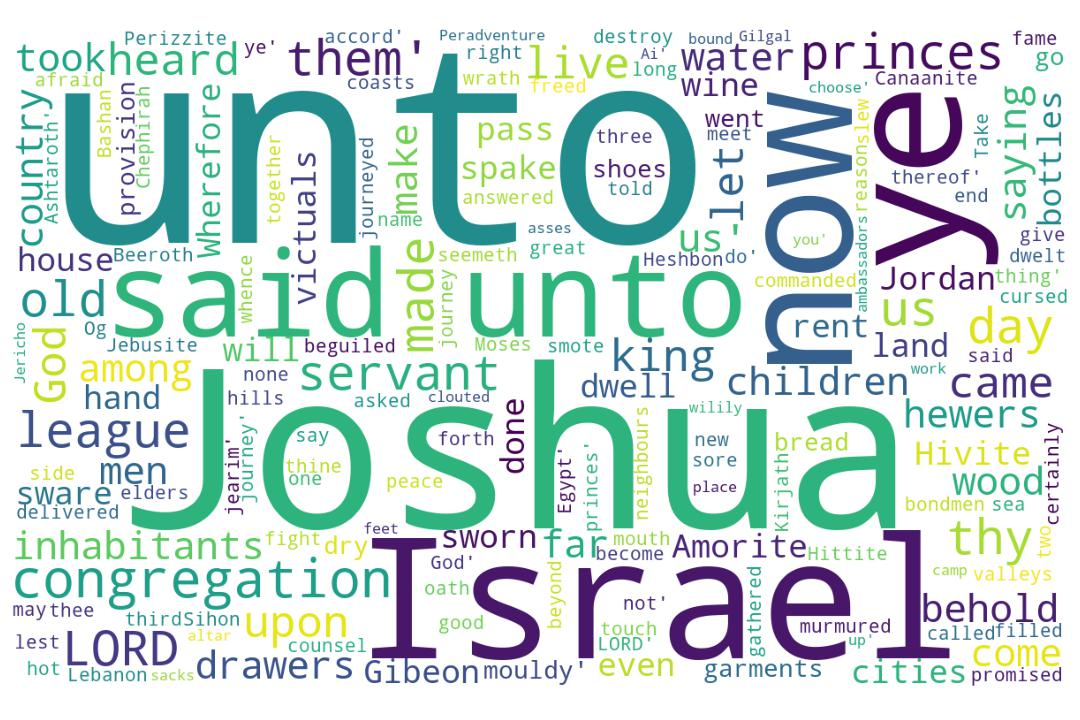
\includegraphics[width=\linewidth]{06OT-Joshua/Joshua9-WordCloud.jpg}
  \caption{Joshua 9 Word Cloud}
  \label{fig:Joshua 9 Word Cloud}
\end{figure}

%%%%%%%%%%%%%%%%%%%%%%%%%%%%%%%%%%%%%%%%%%%%%%%%
\marginpar{\scriptsize \centering \fcolorbox{bone}{lime}{\textbf{A SNEAKY DEAL}}\\ (Joshua 9)
\begin{compactenum}[I.][8]
    \item The \textbf{Dread} \index[scripture]{Joshua!Jsh 09:02} \index[scripture]{Joshua!Jsh 09:24}  (Jsh 9:2, 24) 
    \item The Things that Have been  \textbf{Done} \index[scripture]{Joshua!Jsh 09:03}  
    \item The \textbf{Deception} \index[scripture]{Joshua!Jsh 09:04}  (Jsh 9:4) 
    \item The \textbf{Deal} \index[scripture]{Joshua!Jsh 09:15}  (Jsh 9:15) 
    \item Three \textbf{Days} to Know the Truth \index[scripture]{Joshua!Jsh 09:16--17}  (Jsh 9:16--17) 
    \item \textbf{Drawers and Hewers} \index[scripture]{Joshua!Jsh 09:21}\index[scripture]{Joshua!Jsh 09:23}\index[scripture]{Joshua!Jsh 09:27}  (Jsh 9:21, 23, 27) 
    \item The \textbf{Destruction} \index[scripture]{Joshua!Jsh 09:24} \index[scripture]{Joshua!Jsh 09:24}  (Jsh 9:24) 
    \item \textbf{Delivery} from Revenge \index[scripture]{Joshua!Jsh 09:26}  (Jsh 9:26) 
\end{compactenum}}

%%%%%%%%%%%%%%%%%%%%%%%%%%%%%%%%%%%%%%%%%%%%%%%%
\footnote{\textcolor[rgb]{0.00,0.25,0.00}{\hyperlink{TOC}{Return to end of Table of Contents.}}}\footnote{\href{https://audiobible.com/bible/joshua_9.html}{\textcolor[cmyk]{0.99998,1,0,0}{Joshua 9 Audio}}}\textcolor[cmyk]{0.99998,1,0,0}{And it came to pass, when all the kings which \emph{were} on this side Jordan, in the hills, and in the valleys, and in all the coasts \fcolorbox{bone}{bone}{of the} great sea over against Lebanon, the Hittite, and the Amorite, the Canaanite, the Perizzite, the Hivite, and the Jebusite, heard \emph{thereof};}
[2] \textcolor[cmyk]{0.99998,1,0,0}{That they \fcolorbox{bone}{lime}{gathered} themselves together, to fight with Joshua and with Israel, with one accord.}\\
\\
\P \textcolor[cmyk]{0.99998,1,0,0}{And when the inhabitants of Gibeon heard what Joshua had \fcolorbox{bone}{lime}{done} unto Jericho and to Ai,}\
[4] \textcolor[cmyk]{0.99998,1,0,0}{They did work wilily, and went and made as if they had been ambassadors, and took old sacks upon their asses, and wine bottles, old, and rent, and bound up;}
[5] \textcolor[cmyk]{0.99998,1,0,0}{And \fcolorbox{bone}{lime}{old shoes} and clouted upon their feet, and \fcolorbox{bone}{lime}{old garments} upon them; and all the bread of their provision was dry \emph{and} \fcolorbox{bone}{lime}{mouldy}.}
[6] \textcolor[cmyk]{0.99998,1,0,0}{And they went to Joshua unto the camp at Gilgal, and said unto him, and to the men of Israel, We be come from a far country: now therefore make ye a league with us.}
[7] \textcolor[cmyk]{0.99998,1,0,0}{And the men of Israel said unto the Hivites, Peradventure ye dwell among us; and how shall we make a league with you?}
[8] \textcolor[cmyk]{0.99998,1,0,0}{And they said unto Joshua, We \emph{are} thy servants. And Joshua said unto them, Who \emph{are} ye? and from whence come ye?}
[9] \textcolor[cmyk]{0.99998,1,0,0}{And they said unto him, From a very far country thy servants are come because \fcolorbox{bone}{bone}{of the} name \fcolorbox{bone}{bone}{of the} LORD thy God: for we have heard the fame of him, and all that he did in Egypt,}
[10] \textcolor[cmyk]{0.99998,1,0,0}{And all that he did to the two kings \fcolorbox{bone}{bone}{of the} Amorites, that \emph{were} beyond Jordan, to Sihon king of Heshbon, and to Og king of Bashan, which \emph{was} at Ashtaroth.}
[11] \textcolor[cmyk]{0.99998,1,0,0}{Wherefore our elders and all the inhabitants of our country spake to us, saying, Take victuals with you for the journey, and go to meet them, and say unto them, We \emph{are} your servants: therefore now make ye a league with us.}
[12] \textcolor[cmyk]{0.99998,1,0,0}{This our bread we took hot \emph{for} our provision out of our houses on the day we came forth to go unto you; but now, behold, it is dry, and it is mouldy:}
[13] \textcolor[cmyk]{0.99998,1,0,0}{And these bottles of wine, which we filled, \emph{were} new; and, behold, they be rent: and these our garments and our shoes are become old by reason \fcolorbox{bone}{bone}{of the} very long journey.}
[14] \textcolor[cmyk]{0.99998,1,0,0}{And the men took of their victuals, and asked not \emph{counsel} at the mouth \fcolorbox{bone}{bone}{of the} LORD.}
[15] \textcolor[cmyk]{0.99998,1,0,0}{And Joshua made \fcolorbox{bone}{lime}{peace} with them, and made a \fcolorbox{bone}{lime}{league} with them, to let them live: and the princes \fcolorbox{bone}{bone}{of the} congregation sware unto them.}\\
\\
\P \textcolor[cmyk]{0.99998,1,0,0}{And it came to pass at the end of \fcolorbox{bone}{lime}{three days} after they had made a league with them, that they heard that they \emph{were} their neighbours, and \emph{that} they dwelt among them.}
[17] \textcolor[cmyk]{0.99998,1,0,0}{And the children of Israel journeyed, and came unto their cities on the third day. Now their cities \emph{were} Gibeon, and Chephirah, and Beeroth, and Kirjath-jearim.}
[18] \textcolor[cmyk]{0.99998,1,0,0}{And the children of Israel smote them not, because the princes \fcolorbox{bone}{bone}{of the} congregation had sworn unto them by the LORD God of Israel. And all the congregation murmured against the princes.}
[19] \textcolor[cmyk]{0.99998,1,0,0}{But all the princes said unto all the congregation, We have sworn unto them by the LORD God of Israel: now therefore we may not touch them.}
[20] \textcolor[cmyk]{0.99998,1,0,0}{This we will do to them; we will even let them live, lest wrath be upon us, because \fcolorbox{bone}{bone}{of the} oath which we sware unto them.}
[21] \textcolor[cmyk]{0.99998,1,0,0}{And the princes said unto them, Let them live; but let them be \fcolorbox{bone}{lime}{hewers} of wood and \fcolorbox{bone}{lime}{drawers} of water unto all the congregation; as the princes had promised them.}\\
\\
\P \textcolor[cmyk]{0.99998,1,0,0}{And Joshua called for them, and he spake unto them, saying, Wherefore have ye beguiled us, saying, We \emph{are} very far from you; when ye dwell among us?}
[23] \textcolor[cmyk]{0.99998,1,0,0}{Now therefore ye \emph{are} cursed, and there shall none of you be freed from being \fcolorbox{bone}{lime}{bondmen}, and \fcolorbox{bone}{lime}{hewers} of wood and \fcolorbox{bone}{lime}{drawers} of water for the house of my God.}
[24] \textcolor[cmyk]{0.99998,1,0,0}{And they answered Joshua, and said, Because it was certainly told thy servants, how that the LORD thy God commanded his servant Moses to give you all the land, and to \fcolorbox{bone}{lime}{destroy} all the inhabitants \fcolorbox{bone}{bone}{of the} land from before you, therefore we were sore afraid of our lives \fcolorbox{bone}{lime}{because of you}, and have done this thing.}
[25] \textcolor[cmyk]{0.99998,1,0,0}{And now, behold, we \emph{are} in thine hand: as it seemeth good and right unto thee to do unto us, do.}
[26] \textcolor[cmyk]{0.99998,1,0,0}{And so did he unto them, and delivered them out \fcolorbox{bone}{bone}{of the} hand \fcolorbox{bone}{bone}{of the} children of Israel, that they slew them not.}
[27] \textcolor[cmyk]{0.99998,1,0,0}{And Joshua made them that day \fcolorbox{bone}{lime}{hewers} of wood and \fcolorbox{bone}{lime}{drawers} of water for the congregation, and for the altar \fcolorbox{bone}{bone}{of the} LORD, even unto this day, in the place which he should choose.}


\index[NWIV]{50!Joshua!Jos 9:1}\index[AWIP]{And!Joshua!Jos 9:1}\index[AWIP]{it!Joshua!Jos 9:1}\index[AWIP]{came!Joshua!Jos 9:1}\index[AWIP]{to!Joshua!Jos 9:1}\index[AWIP]{pass!Joshua!Jos 9:1}\index[AWIP]{when!Joshua!Jos 9:1}\index[AWIP]{all!Joshua!Jos 9:1}\index[AWIP]{all!Joshua!Jos 9:1 (2)}\index[AWIP]{the!Joshua!Jos 9:1}\index[AWIP]{the!Joshua!Jos 9:1 (2)}\index[AWIP]{the!Joshua!Jos 9:1 (3)}\index[AWIP]{the!Joshua!Jos 9:1 (4)}\index[AWIP]{the!Joshua!Jos 9:1 (5)}\index[AWIP]{the!Joshua!Jos 9:1 (6)}\index[AWIP]{the!Joshua!Jos 9:1 (7)}\index[AWIP]{the!Joshua!Jos 9:1 (8)}\index[AWIP]{the!Joshua!Jos 9:1 (9)}\index[AWIP]{the!Joshua!Jos 9:1 (10)}\index[AWIP]{the!Joshua!Jos 9:1 (11)}\index[AWIP]{kings!Joshua!Jos 9:1}\index[AWIP]{which!Joshua!Jos 9:1}\index[AWIP]{\emph{were}!Joshua!Jos 9:1}\index[AWIP]{on!Joshua!Jos 9:1}\index[AWIP]{this!Joshua!Jos 9:1}\index[AWIP]{side!Joshua!Jos 9:1}\index[AWIP]{Jordan!Joshua!Jos 9:1}\index[AWIP]{in!Joshua!Jos 9:1}\index[AWIP]{in!Joshua!Jos 9:1 (2)}\index[AWIP]{in!Joshua!Jos 9:1 (3)}\index[AWIP]{hills!Joshua!Jos 9:1}\index[AWIP]{and!Joshua!Jos 9:1}\index[AWIP]{and!Joshua!Jos 9:1 (2)}\index[AWIP]{and!Joshua!Jos 9:1 (3)}\index[AWIP]{and!Joshua!Jos 9:1 (4)}\index[AWIP]{valleys!Joshua!Jos 9:1}\index[AWIP]{coasts!Joshua!Jos 9:1}\index[AWIP]{of!Joshua!Jos 9:1}\index[AWIP]{great!Joshua!Jos 9:1}\index[AWIP]{sea!Joshua!Jos 9:1}\index[AWIP]{over!Joshua!Jos 9:1}\index[AWIP]{against!Joshua!Jos 9:1}\index[AWIP]{Lebanon!Joshua!Jos 9:1}\index[AWIP]{Hittite!Joshua!Jos 9:1}\index[AWIP]{Amorite!Joshua!Jos 9:1}\index[AWIP]{Canaanite!Joshua!Jos 9:1}\index[AWIP]{Perizzite!Joshua!Jos 9:1}\index[AWIP]{Hivite!Joshua!Jos 9:1}\index[AWIP]{Jebusite!Joshua!Jos 9:1}\index[AWIP]{heard!Joshua!Jos 9:1}\index[AWIP]{\emph{thereof}!Joshua!Jos 9:1}\index[AWIP]{\emph{were}!Joshua!Jos 9:1}\index[AWIP]{\emph{thereof}!Joshua!Jos 9:1}

\index[NWIV]{15!Joshua!Jos 9:2}\index[AWIP]{That!Joshua!Jos 9:2}\index[AWIP]{they!Joshua!Jos 9:2}\index[AWIP]{gathered!Joshua!Jos 9:2}\index[AWIP]{themselves!Joshua!Jos 9:2}\index[AWIP]{together!Joshua!Jos 9:2}\index[AWIP]{to!Joshua!Jos 9:2}\index[AWIP]{fight!Joshua!Jos 9:2}\index[AWIP]{with!Joshua!Jos 9:2}\index[AWIP]{with!Joshua!Jos 9:2 (2)}\index[AWIP]{with!Joshua!Jos 9:2 (3)}\index[AWIP]{Joshua!Joshua!Jos 9:2}\index[AWIP]{and!Joshua!Jos 9:2}\index[AWIP]{Israel!Joshua!Jos 9:2}\index[AWIP]{one!Joshua!Jos 9:2}\index[AWIP]{accord!Joshua!Jos 9:2}

\index[NWIV]{16!Joshua!Jos 9:3}\index[AWIP]{And!Joshua!Jos 9:3}\index[AWIP]{when!Joshua!Jos 9:3}\index[AWIP]{the!Joshua!Jos 9:3}\index[AWIP]{inhabitants!Joshua!Jos 9:3}\index[AWIP]{of!Joshua!Jos 9:3}\index[AWIP]{Gibeon!Joshua!Jos 9:3}\index[AWIP]{heard!Joshua!Jos 9:3}\index[AWIP]{what!Joshua!Jos 9:3}\index[AWIP]{Joshua!Joshua!Jos 9:3}\index[AWIP]{had!Joshua!Jos 9:3}\index[AWIP]{done!Joshua!Jos 9:3}\index[AWIP]{unto!Joshua!Jos 9:3}\index[AWIP]{Jericho!Joshua!Jos 9:3}\index[AWIP]{and!Joshua!Jos 9:3}\index[AWIP]{to!Joshua!Jos 9:3}\index[AWIP]{Ai!Joshua!Jos 9:3}

\index[NWIV]{30!Joshua!Jos 9:4}\index[AWIP]{They!Joshua!Jos 9:4}\index[AWIP]{did!Joshua!Jos 9:4}\index[AWIP]{work!Joshua!Jos 9:4}\index[AWIP]{wilily!Joshua!Jos 9:4}\index[AWIP]{and!Joshua!Jos 9:4}\index[AWIP]{and!Joshua!Jos 9:4 (2)}\index[AWIP]{and!Joshua!Jos 9:4 (3)}\index[AWIP]{and!Joshua!Jos 9:4 (4)}\index[AWIP]{and!Joshua!Jos 9:4 (5)}\index[AWIP]{and!Joshua!Jos 9:4 (6)}\index[AWIP]{went!Joshua!Jos 9:4}\index[AWIP]{made!Joshua!Jos 9:4}\index[AWIP]{as!Joshua!Jos 9:4}\index[AWIP]{if!Joshua!Jos 9:4}\index[AWIP]{they!Joshua!Jos 9:4}\index[AWIP]{had!Joshua!Jos 9:4}\index[AWIP]{been!Joshua!Jos 9:4}\index[AWIP]{ambassadors!Joshua!Jos 9:4}\index[AWIP]{took!Joshua!Jos 9:4}\index[AWIP]{old!Joshua!Jos 9:4}\index[AWIP]{old!Joshua!Jos 9:4 (2)}\index[AWIP]{sacks!Joshua!Jos 9:4}\index[AWIP]{upon!Joshua!Jos 9:4}\index[AWIP]{their!Joshua!Jos 9:4}\index[AWIP]{asses!Joshua!Jos 9:4}\index[AWIP]{wine!Joshua!Jos 9:4}\index[AWIP]{bottles!Joshua!Jos 9:4}\index[AWIP]{rent!Joshua!Jos 9:4}\index[AWIP]{bound!Joshua!Jos 9:4}\index[AWIP]{up!Joshua!Jos 9:4}

\index[NWIV]{24!Joshua!Jos 9:5}\index[AWIP]{And!Joshua!Jos 9:5}\index[AWIP]{old!Joshua!Jos 9:5}\index[AWIP]{old!Joshua!Jos 9:5 (2)}\index[AWIP]{shoes!Joshua!Jos 9:5}\index[AWIP]{and!Joshua!Jos 9:5}\index[AWIP]{and!Joshua!Jos 9:5 (2)}\index[AWIP]{and!Joshua!Jos 9:5 (3)}\index[AWIP]{clouted!Joshua!Jos 9:5}\index[AWIP]{upon!Joshua!Jos 9:5}\index[AWIP]{upon!Joshua!Jos 9:5 (2)}\index[AWIP]{their!Joshua!Jos 9:5}\index[AWIP]{their!Joshua!Jos 9:5 (2)}\index[AWIP]{feet!Joshua!Jos 9:5}\index[AWIP]{garments!Joshua!Jos 9:5}\index[AWIP]{them!Joshua!Jos 9:5}\index[AWIP]{all!Joshua!Jos 9:5}\index[AWIP]{the!Joshua!Jos 9:5}\index[AWIP]{bread!Joshua!Jos 9:5}\index[AWIP]{of!Joshua!Jos 9:5}\index[AWIP]{provision!Joshua!Jos 9:5}\index[AWIP]{was!Joshua!Jos 9:5}\index[AWIP]{dry!Joshua!Jos 9:5}\index[AWIP]{\emph{and}!Joshua!Jos 9:5}\index[AWIP]{mouldy!Joshua!Jos 9:5}\index[AWIP]{\emph{and}!Joshua!Jos 9:5}

\index[NWIV]{35!Joshua!Jos 9:6}\index[AWIP]{And!Joshua!Jos 9:6}\index[AWIP]{they!Joshua!Jos 9:6}\index[AWIP]{went!Joshua!Jos 9:6}\index[AWIP]{to!Joshua!Jos 9:6}\index[AWIP]{to!Joshua!Jos 9:6 (2)}\index[AWIP]{Joshua!Joshua!Jos 9:6}\index[AWIP]{unto!Joshua!Jos 9:6}\index[AWIP]{unto!Joshua!Jos 9:6 (2)}\index[AWIP]{the!Joshua!Jos 9:6}\index[AWIP]{the!Joshua!Jos 9:6 (2)}\index[AWIP]{camp!Joshua!Jos 9:6}\index[AWIP]{at!Joshua!Jos 9:6}\index[AWIP]{Gilgal!Joshua!Jos 9:6}\index[AWIP]{and!Joshua!Jos 9:6}\index[AWIP]{and!Joshua!Jos 9:6 (2)}\index[AWIP]{said!Joshua!Jos 9:6}\index[AWIP]{him!Joshua!Jos 9:6}\index[AWIP]{men!Joshua!Jos 9:6}\index[AWIP]{of!Joshua!Jos 9:6}\index[AWIP]{Israel!Joshua!Jos 9:6}\index[AWIP]{We!Joshua!Jos 9:6}\index[AWIP]{be!Joshua!Jos 9:6}\index[AWIP]{come!Joshua!Jos 9:6}\index[AWIP]{from!Joshua!Jos 9:6}\index[AWIP]{a!Joshua!Jos 9:6}\index[AWIP]{a!Joshua!Jos 9:6 (2)}\index[AWIP]{far!Joshua!Jos 9:6}\index[AWIP]{country!Joshua!Jos 9:6}\index[AWIP]{now!Joshua!Jos 9:6}\index[AWIP]{therefore!Joshua!Jos 9:6}\index[AWIP]{make!Joshua!Jos 9:6}\index[AWIP]{ye!Joshua!Jos 9:6}\index[AWIP]{league!Joshua!Jos 9:6}\index[AWIP]{with!Joshua!Jos 9:6}\index[AWIP]{us!Joshua!Jos 9:6}

\index[NWIV]{23!Joshua!Jos 9:7}\index[AWIP]{And!Joshua!Jos 9:7}\index[AWIP]{the!Joshua!Jos 9:7}\index[AWIP]{the!Joshua!Jos 9:7 (2)}\index[AWIP]{men!Joshua!Jos 9:7}\index[AWIP]{of!Joshua!Jos 9:7}\index[AWIP]{Israel!Joshua!Jos 9:7}\index[AWIP]{said!Joshua!Jos 9:7}\index[AWIP]{unto!Joshua!Jos 9:7}\index[AWIP]{Hivites!Joshua!Jos 9:7}\index[AWIP]{Peradventure!Joshua!Jos 9:7}\index[AWIP]{ye!Joshua!Jos 9:7}\index[AWIP]{dwell!Joshua!Jos 9:7}\index[AWIP]{among!Joshua!Jos 9:7}\index[AWIP]{us!Joshua!Jos 9:7}\index[AWIP]{and!Joshua!Jos 9:7}\index[AWIP]{how!Joshua!Jos 9:7}\index[AWIP]{shall!Joshua!Jos 9:7}\index[AWIP]{we!Joshua!Jos 9:7}\index[AWIP]{make!Joshua!Jos 9:7}\index[AWIP]{a!Joshua!Jos 9:7}\index[AWIP]{league!Joshua!Jos 9:7}\index[AWIP]{with!Joshua!Jos 9:7}\index[AWIP]{you?!Joshua!Jos 9:7}

\index[NWIV]{22!Joshua!Jos 9:8}\index[AWIP]{And!Joshua!Jos 9:8}\index[AWIP]{And!Joshua!Jos 9:8 (2)}\index[AWIP]{they!Joshua!Jos 9:8}\index[AWIP]{said!Joshua!Jos 9:8}\index[AWIP]{said!Joshua!Jos 9:8 (2)}\index[AWIP]{unto!Joshua!Jos 9:8}\index[AWIP]{unto!Joshua!Jos 9:8 (2)}\index[AWIP]{Joshua!Joshua!Jos 9:8}\index[AWIP]{Joshua!Joshua!Jos 9:8 (2)}\index[AWIP]{We!Joshua!Jos 9:8}\index[AWIP]{\emph{are}!Joshua!Jos 9:8}\index[AWIP]{\emph{are}!Joshua!Jos 9:8 (2)}\index[AWIP]{thy!Joshua!Jos 9:8}\index[AWIP]{servants!Joshua!Jos 9:8}\index[AWIP]{them!Joshua!Jos 9:8}\index[AWIP]{Who!Joshua!Jos 9:8}\index[AWIP]{ye?!Joshua!Jos 9:8}\index[AWIP]{ye?!Joshua!Jos 9:8 (2)}\index[AWIP]{and!Joshua!Jos 9:8}\index[AWIP]{from!Joshua!Jos 9:8}\index[AWIP]{whence!Joshua!Jos 9:8}\index[AWIP]{come!Joshua!Jos 9:8}\index[AWIP]{\emph{are}!Joshua!Jos 9:8}\index[AWIP]{\emph{are}!Joshua!Jos 9:8 (2)}

\index[NWIV]{38!Joshua!Jos 9:9}\index[AWIP]{And!Joshua!Jos 9:9}\index[AWIP]{they!Joshua!Jos 9:9}\index[AWIP]{said!Joshua!Jos 9:9}\index[AWIP]{unto!Joshua!Jos 9:9}\index[AWIP]{him!Joshua!Jos 9:9}\index[AWIP]{him!Joshua!Jos 9:9 (2)}\index[AWIP]{From!Joshua!Jos 9:9}\index[AWIP]{a!Joshua!Jos 9:9}\index[AWIP]{very!Joshua!Jos 9:9}\index[AWIP]{far!Joshua!Jos 9:9}\index[AWIP]{country!Joshua!Jos 9:9}\index[AWIP]{thy!Joshua!Jos 9:9}\index[AWIP]{thy!Joshua!Jos 9:9 (2)}\index[AWIP]{servants!Joshua!Jos 9:9}\index[AWIP]{are!Joshua!Jos 9:9}\index[AWIP]{come!Joshua!Jos 9:9}\index[AWIP]{because!Joshua!Jos 9:9}\index[AWIP]{of!Joshua!Jos 9:9}\index[AWIP]{of!Joshua!Jos 9:9 (2)}\index[AWIP]{of!Joshua!Jos 9:9 (3)}\index[AWIP]{the!Joshua!Jos 9:9}\index[AWIP]{the!Joshua!Jos 9:9 (2)}\index[AWIP]{the!Joshua!Jos 9:9 (3)}\index[AWIP]{name!Joshua!Jos 9:9}\index[AWIP]{LORD!Joshua!Jos 9:9}\index[AWIP]{God!Joshua!Jos 9:9}\index[AWIP]{for!Joshua!Jos 9:9}\index[AWIP]{we!Joshua!Jos 9:9}\index[AWIP]{have!Joshua!Jos 9:9}\index[AWIP]{heard!Joshua!Jos 9:9}\index[AWIP]{fame!Joshua!Jos 9:9}\index[AWIP]{and!Joshua!Jos 9:9}\index[AWIP]{all!Joshua!Jos 9:9}\index[AWIP]{that!Joshua!Jos 9:9}\index[AWIP]{he!Joshua!Jos 9:9}\index[AWIP]{did!Joshua!Jos 9:9}\index[AWIP]{in!Joshua!Jos 9:9}\index[AWIP]{Egypt!Joshua!Jos 9:9}

\index[NWIV]{31!Joshua!Jos 9:10}\index[AWIP]{And!Joshua!Jos 9:10}\index[AWIP]{all!Joshua!Jos 9:10}\index[AWIP]{that!Joshua!Jos 9:10}\index[AWIP]{that!Joshua!Jos 9:10 (2)}\index[AWIP]{he!Joshua!Jos 9:10}\index[AWIP]{did!Joshua!Jos 9:10}\index[AWIP]{to!Joshua!Jos 9:10}\index[AWIP]{to!Joshua!Jos 9:10 (2)}\index[AWIP]{to!Joshua!Jos 9:10 (3)}\index[AWIP]{the!Joshua!Jos 9:10}\index[AWIP]{the!Joshua!Jos 9:10 (2)}\index[AWIP]{two!Joshua!Jos 9:10}\index[AWIP]{kings!Joshua!Jos 9:10}\index[AWIP]{of!Joshua!Jos 9:10}\index[AWIP]{of!Joshua!Jos 9:10 (2)}\index[AWIP]{of!Joshua!Jos 9:10 (3)}\index[AWIP]{Amorites!Joshua!Jos 9:10}\index[AWIP]{\emph{were}!Joshua!Jos 9:10}\index[AWIP]{beyond!Joshua!Jos 9:10}\index[AWIP]{Jordan!Joshua!Jos 9:10}\index[AWIP]{Sihon!Joshua!Jos 9:10}\index[AWIP]{king!Joshua!Jos 9:10}\index[AWIP]{king!Joshua!Jos 9:10 (2)}\index[AWIP]{Heshbon!Joshua!Jos 9:10}\index[AWIP]{and!Joshua!Jos 9:10}\index[AWIP]{Og!Joshua!Jos 9:10}\index[AWIP]{Bashan!Joshua!Jos 9:10}\index[AWIP]{which!Joshua!Jos 9:10}\index[AWIP]{\emph{was}!Joshua!Jos 9:10}\index[AWIP]{at!Joshua!Jos 9:10}\index[AWIP]{Ashtaroth!Joshua!Jos 9:10}\index[AWIP]{\emph{were}!Joshua!Jos 9:10}\index[AWIP]{\emph{was}!Joshua!Jos 9:10}

\index[NWIV]{42!Joshua!Jos 9:11}\index[AWIP]{Wherefore!Joshua!Jos 9:11}\index[AWIP]{our!Joshua!Jos 9:11}\index[AWIP]{our!Joshua!Jos 9:11 (2)}\index[AWIP]{elders!Joshua!Jos 9:11}\index[AWIP]{and!Joshua!Jos 9:11}\index[AWIP]{and!Joshua!Jos 9:11 (2)}\index[AWIP]{and!Joshua!Jos 9:11 (3)}\index[AWIP]{all!Joshua!Jos 9:11}\index[AWIP]{the!Joshua!Jos 9:11}\index[AWIP]{the!Joshua!Jos 9:11 (2)}\index[AWIP]{inhabitants!Joshua!Jos 9:11}\index[AWIP]{of!Joshua!Jos 9:11}\index[AWIP]{country!Joshua!Jos 9:11}\index[AWIP]{spake!Joshua!Jos 9:11}\index[AWIP]{to!Joshua!Jos 9:11}\index[AWIP]{to!Joshua!Jos 9:11 (2)}\index[AWIP]{us!Joshua!Jos 9:11}\index[AWIP]{us!Joshua!Jos 9:11 (2)}\index[AWIP]{saying!Joshua!Jos 9:11}\index[AWIP]{Take!Joshua!Jos 9:11}\index[AWIP]{victuals!Joshua!Jos 9:11}\index[AWIP]{with!Joshua!Jos 9:11}\index[AWIP]{with!Joshua!Jos 9:11 (2)}\index[AWIP]{you!Joshua!Jos 9:11}\index[AWIP]{for!Joshua!Jos 9:11}\index[AWIP]{journey!Joshua!Jos 9:11}\index[AWIP]{go!Joshua!Jos 9:11}\index[AWIP]{meet!Joshua!Jos 9:11}\index[AWIP]{them!Joshua!Jos 9:11}\index[AWIP]{them!Joshua!Jos 9:11 (2)}\index[AWIP]{say!Joshua!Jos 9:11}\index[AWIP]{unto!Joshua!Jos 9:11}\index[AWIP]{We!Joshua!Jos 9:11}\index[AWIP]{\emph{are}!Joshua!Jos 9:11}\index[AWIP]{your!Joshua!Jos 9:11}\index[AWIP]{servants!Joshua!Jos 9:11}\index[AWIP]{therefore!Joshua!Jos 9:11}\index[AWIP]{now!Joshua!Jos 9:11}\index[AWIP]{make!Joshua!Jos 9:11}\index[AWIP]{ye!Joshua!Jos 9:11}\index[AWIP]{a!Joshua!Jos 9:11}\index[AWIP]{league!Joshua!Jos 9:11}\index[AWIP]{\emph{are}!Joshua!Jos 9:11}

\index[NWIV]{33!Joshua!Jos 9:12}\index[AWIP]{This!Joshua!Jos 9:12}\index[AWIP]{our!Joshua!Jos 9:12}\index[AWIP]{our!Joshua!Jos 9:12 (2)}\index[AWIP]{our!Joshua!Jos 9:12 (3)}\index[AWIP]{bread!Joshua!Jos 9:12}\index[AWIP]{we!Joshua!Jos 9:12}\index[AWIP]{we!Joshua!Jos 9:12 (2)}\index[AWIP]{took!Joshua!Jos 9:12}\index[AWIP]{hot!Joshua!Jos 9:12}\index[AWIP]{\emph{for}!Joshua!Jos 9:12}\index[AWIP]{provision!Joshua!Jos 9:12}\index[AWIP]{out!Joshua!Jos 9:12}\index[AWIP]{of!Joshua!Jos 9:12}\index[AWIP]{houses!Joshua!Jos 9:12}\index[AWIP]{on!Joshua!Jos 9:12}\index[AWIP]{the!Joshua!Jos 9:12}\index[AWIP]{day!Joshua!Jos 9:12}\index[AWIP]{came!Joshua!Jos 9:12}\index[AWIP]{forth!Joshua!Jos 9:12}\index[AWIP]{to!Joshua!Jos 9:12}\index[AWIP]{go!Joshua!Jos 9:12}\index[AWIP]{unto!Joshua!Jos 9:12}\index[AWIP]{you!Joshua!Jos 9:12}\index[AWIP]{but!Joshua!Jos 9:12}\index[AWIP]{now!Joshua!Jos 9:12}\index[AWIP]{behold!Joshua!Jos 9:12}\index[AWIP]{it!Joshua!Jos 9:12}\index[AWIP]{it!Joshua!Jos 9:12 (2)}\index[AWIP]{is!Joshua!Jos 9:12}\index[AWIP]{is!Joshua!Jos 9:12 (2)}\index[AWIP]{dry!Joshua!Jos 9:12}\index[AWIP]{and!Joshua!Jos 9:12}\index[AWIP]{mouldy!Joshua!Jos 9:12}\index[AWIP]{\emph{for}!Joshua!Jos 9:12}

\index[NWIV]{32!Joshua!Jos 9:13}\index[AWIP]{And!Joshua!Jos 9:13}\index[AWIP]{these!Joshua!Jos 9:13}\index[AWIP]{these!Joshua!Jos 9:13 (2)}\index[AWIP]{bottles!Joshua!Jos 9:13}\index[AWIP]{of!Joshua!Jos 9:13}\index[AWIP]{of!Joshua!Jos 9:13 (2)}\index[AWIP]{wine!Joshua!Jos 9:13}\index[AWIP]{which!Joshua!Jos 9:13}\index[AWIP]{we!Joshua!Jos 9:13}\index[AWIP]{filled!Joshua!Jos 9:13}\index[AWIP]{\emph{were}!Joshua!Jos 9:13}\index[AWIP]{new!Joshua!Jos 9:13}\index[AWIP]{and!Joshua!Jos 9:13}\index[AWIP]{and!Joshua!Jos 9:13 (2)}\index[AWIP]{and!Joshua!Jos 9:13 (3)}\index[AWIP]{behold!Joshua!Jos 9:13}\index[AWIP]{they!Joshua!Jos 9:13}\index[AWIP]{be!Joshua!Jos 9:13}\index[AWIP]{rent!Joshua!Jos 9:13}\index[AWIP]{our!Joshua!Jos 9:13}\index[AWIP]{our!Joshua!Jos 9:13 (2)}\index[AWIP]{garments!Joshua!Jos 9:13}\index[AWIP]{shoes!Joshua!Jos 9:13}\index[AWIP]{are!Joshua!Jos 9:13}\index[AWIP]{become!Joshua!Jos 9:13}\index[AWIP]{old!Joshua!Jos 9:13}\index[AWIP]{by!Joshua!Jos 9:13}\index[AWIP]{reason!Joshua!Jos 9:13}\index[AWIP]{the!Joshua!Jos 9:13}\index[AWIP]{very!Joshua!Jos 9:13}\index[AWIP]{long!Joshua!Jos 9:13}\index[AWIP]{journey!Joshua!Jos 9:13}\index[AWIP]{\emph{were}!Joshua!Jos 9:13}

\index[NWIV]{17!Joshua!Jos 9:14}\index[AWIP]{And!Joshua!Jos 9:14}\index[AWIP]{the!Joshua!Jos 9:14}\index[AWIP]{the!Joshua!Jos 9:14 (2)}\index[AWIP]{the!Joshua!Jos 9:14 (3)}\index[AWIP]{men!Joshua!Jos 9:14}\index[AWIP]{took!Joshua!Jos 9:14}\index[AWIP]{of!Joshua!Jos 9:14}\index[AWIP]{of!Joshua!Jos 9:14 (2)}\index[AWIP]{their!Joshua!Jos 9:14}\index[AWIP]{victuals!Joshua!Jos 9:14}\index[AWIP]{and!Joshua!Jos 9:14}\index[AWIP]{asked!Joshua!Jos 9:14}\index[AWIP]{not!Joshua!Jos 9:14}\index[AWIP]{\emph{counsel}!Joshua!Jos 9:14}\index[AWIP]{at!Joshua!Jos 9:14}\index[AWIP]{mouth!Joshua!Jos 9:14}\index[AWIP]{LORD!Joshua!Jos 9:14}\index[AWIP]{\emph{counsel}!Joshua!Jos 9:14}

\index[NWIV]{25!Joshua!Jos 9:15}\index[AWIP]{And!Joshua!Jos 9:15}\index[AWIP]{Joshua!Joshua!Jos 9:15}\index[AWIP]{made!Joshua!Jos 9:15}\index[AWIP]{made!Joshua!Jos 9:15 (2)}\index[AWIP]{peace!Joshua!Jos 9:15}\index[AWIP]{with!Joshua!Jos 9:15}\index[AWIP]{with!Joshua!Jos 9:15 (2)}\index[AWIP]{them!Joshua!Jos 9:15}\index[AWIP]{them!Joshua!Jos 9:15 (2)}\index[AWIP]{them!Joshua!Jos 9:15 (3)}\index[AWIP]{them!Joshua!Jos 9:15 (4)}\index[AWIP]{and!Joshua!Jos 9:15}\index[AWIP]{and!Joshua!Jos 9:15 (2)}\index[AWIP]{a!Joshua!Jos 9:15}\index[AWIP]{league!Joshua!Jos 9:15}\index[AWIP]{to!Joshua!Jos 9:15}\index[AWIP]{let!Joshua!Jos 9:15}\index[AWIP]{live!Joshua!Jos 9:15}\index[AWIP]{the!Joshua!Jos 9:15}\index[AWIP]{the!Joshua!Jos 9:15 (2)}\index[AWIP]{princes!Joshua!Jos 9:15}\index[AWIP]{of!Joshua!Jos 9:15}\index[AWIP]{congregation!Joshua!Jos 9:15}\index[AWIP]{sware!Joshua!Jos 9:15}\index[AWIP]{unto!Joshua!Jos 9:15}

\index[NWIV]{33!Joshua!Jos 9:16}\index[AWIP]{And!Joshua!Jos 9:16}\index[AWIP]{it!Joshua!Jos 9:16}\index[AWIP]{came!Joshua!Jos 9:16}\index[AWIP]{to!Joshua!Jos 9:16}\index[AWIP]{pass!Joshua!Jos 9:16}\index[AWIP]{at!Joshua!Jos 9:16}\index[AWIP]{the!Joshua!Jos 9:16}\index[AWIP]{end!Joshua!Jos 9:16}\index[AWIP]{of!Joshua!Jos 9:16}\index[AWIP]{three!Joshua!Jos 9:16}\index[AWIP]{days!Joshua!Jos 9:16}\index[AWIP]{after!Joshua!Jos 9:16}\index[AWIP]{they!Joshua!Jos 9:16}\index[AWIP]{they!Joshua!Jos 9:16 (2)}\index[AWIP]{they!Joshua!Jos 9:16 (3)}\index[AWIP]{they!Joshua!Jos 9:16 (4)}\index[AWIP]{had!Joshua!Jos 9:16}\index[AWIP]{made!Joshua!Jos 9:16}\index[AWIP]{a!Joshua!Jos 9:16}\index[AWIP]{league!Joshua!Jos 9:16}\index[AWIP]{with!Joshua!Jos 9:16}\index[AWIP]{them!Joshua!Jos 9:16}\index[AWIP]{them!Joshua!Jos 9:16 (2)}\index[AWIP]{that!Joshua!Jos 9:16}\index[AWIP]{that!Joshua!Jos 9:16 (2)}\index[AWIP]{heard!Joshua!Jos 9:16}\index[AWIP]{\emph{were}!Joshua!Jos 9:16}\index[AWIP]{their!Joshua!Jos 9:16}\index[AWIP]{neighbours!Joshua!Jos 9:16}\index[AWIP]{and!Joshua!Jos 9:16}\index[AWIP]{\emph{that}!Joshua!Jos 9:16}\index[AWIP]{dwelt!Joshua!Jos 9:16}\index[AWIP]{among!Joshua!Jos 9:16}\index[AWIP]{\emph{were}!Joshua!Jos 9:16}\index[AWIP]{\emph{that}!Joshua!Jos 9:16}

\index[NWIV]{26!Joshua!Jos 9:17}\index[AWIP]{And!Joshua!Jos 9:17}\index[AWIP]{the!Joshua!Jos 9:17}\index[AWIP]{the!Joshua!Jos 9:17 (2)}\index[AWIP]{children!Joshua!Jos 9:17}\index[AWIP]{of!Joshua!Jos 9:17}\index[AWIP]{Israel!Joshua!Jos 9:17}\index[AWIP]{journeyed!Joshua!Jos 9:17}\index[AWIP]{and!Joshua!Jos 9:17}\index[AWIP]{and!Joshua!Jos 9:17 (2)}\index[AWIP]{and!Joshua!Jos 9:17 (3)}\index[AWIP]{and!Joshua!Jos 9:17 (4)}\index[AWIP]{came!Joshua!Jos 9:17}\index[AWIP]{unto!Joshua!Jos 9:17}\index[AWIP]{their!Joshua!Jos 9:17}\index[AWIP]{their!Joshua!Jos 9:17 (2)}\index[AWIP]{cities!Joshua!Jos 9:17}\index[AWIP]{cities!Joshua!Jos 9:17 (2)}\index[AWIP]{on!Joshua!Jos 9:17}\index[AWIP]{third!Joshua!Jos 9:17}\index[AWIP]{day!Joshua!Jos 9:17}\index[AWIP]{Now!Joshua!Jos 9:17}\index[AWIP]{\emph{were}!Joshua!Jos 9:17}\index[AWIP]{Gibeon!Joshua!Jos 9:17}\index[AWIP]{Chephirah!Joshua!Jos 9:17}\index[AWIP]{Beeroth!Joshua!Jos 9:17}\index[AWIP]{Kirjath-jearim!Joshua!Jos 9:17}\index[AWIP]{\emph{were}!Joshua!Jos 9:17}

\index[NWIV]{32!Joshua!Jos 9:18}\index[AWIP]{And!Joshua!Jos 9:18}\index[AWIP]{And!Joshua!Jos 9:18 (2)}\index[AWIP]{the!Joshua!Jos 9:18}\index[AWIP]{the!Joshua!Jos 9:18 (2)}\index[AWIP]{the!Joshua!Jos 9:18 (3)}\index[AWIP]{the!Joshua!Jos 9:18 (4)}\index[AWIP]{the!Joshua!Jos 9:18 (5)}\index[AWIP]{the!Joshua!Jos 9:18 (6)}\index[AWIP]{children!Joshua!Jos 9:18}\index[AWIP]{of!Joshua!Jos 9:18}\index[AWIP]{of!Joshua!Jos 9:18 (2)}\index[AWIP]{of!Joshua!Jos 9:18 (3)}\index[AWIP]{Israel!Joshua!Jos 9:18}\index[AWIP]{Israel!Joshua!Jos 9:18 (2)}\index[AWIP]{smote!Joshua!Jos 9:18}\index[AWIP]{them!Joshua!Jos 9:18}\index[AWIP]{them!Joshua!Jos 9:18 (2)}\index[AWIP]{not!Joshua!Jos 9:18}\index[AWIP]{because!Joshua!Jos 9:18}\index[AWIP]{princes!Joshua!Jos 9:18}\index[AWIP]{princes!Joshua!Jos 9:18 (2)}\index[AWIP]{congregation!Joshua!Jos 9:18}\index[AWIP]{congregation!Joshua!Jos 9:18 (2)}\index[AWIP]{had!Joshua!Jos 9:18}\index[AWIP]{sworn!Joshua!Jos 9:18}\index[AWIP]{unto!Joshua!Jos 9:18}\index[AWIP]{by!Joshua!Jos 9:18}\index[AWIP]{LORD!Joshua!Jos 9:18}\index[AWIP]{God!Joshua!Jos 9:18}\index[AWIP]{all!Joshua!Jos 9:18}\index[AWIP]{murmured!Joshua!Jos 9:18}\index[AWIP]{against!Joshua!Jos 9:18}

\index[NWIV]{27!Joshua!Jos 9:19}\index[AWIP]{But!Joshua!Jos 9:19}\index[AWIP]{all!Joshua!Jos 9:19}\index[AWIP]{all!Joshua!Jos 9:19 (2)}\index[AWIP]{the!Joshua!Jos 9:19}\index[AWIP]{the!Joshua!Jos 9:19 (2)}\index[AWIP]{the!Joshua!Jos 9:19 (3)}\index[AWIP]{princes!Joshua!Jos 9:19}\index[AWIP]{said!Joshua!Jos 9:19}\index[AWIP]{unto!Joshua!Jos 9:19}\index[AWIP]{unto!Joshua!Jos 9:19 (2)}\index[AWIP]{congregation!Joshua!Jos 9:19}\index[AWIP]{We!Joshua!Jos 9:19}\index[AWIP]{have!Joshua!Jos 9:19}\index[AWIP]{sworn!Joshua!Jos 9:19}\index[AWIP]{them!Joshua!Jos 9:19}\index[AWIP]{them!Joshua!Jos 9:19 (2)}\index[AWIP]{by!Joshua!Jos 9:19}\index[AWIP]{LORD!Joshua!Jos 9:19}\index[AWIP]{God!Joshua!Jos 9:19}\index[AWIP]{of!Joshua!Jos 9:19}\index[AWIP]{Israel!Joshua!Jos 9:19}\index[AWIP]{now!Joshua!Jos 9:19}\index[AWIP]{therefore!Joshua!Jos 9:19}\index[AWIP]{we!Joshua!Jos 9:19}\index[AWIP]{may!Joshua!Jos 9:19}\index[AWIP]{not!Joshua!Jos 9:19}\index[AWIP]{touch!Joshua!Jos 9:19}

\index[NWIV]{26!Joshua!Jos 9:20}\index[AWIP]{This!Joshua!Jos 9:20}\index[AWIP]{we!Joshua!Jos 9:20}\index[AWIP]{we!Joshua!Jos 9:20 (2)}\index[AWIP]{we!Joshua!Jos 9:20 (3)}\index[AWIP]{will!Joshua!Jos 9:20}\index[AWIP]{will!Joshua!Jos 9:20 (2)}\index[AWIP]{do!Joshua!Jos 9:20}\index[AWIP]{to!Joshua!Jos 9:20}\index[AWIP]{them!Joshua!Jos 9:20}\index[AWIP]{them!Joshua!Jos 9:20 (2)}\index[AWIP]{them!Joshua!Jos 9:20 (3)}\index[AWIP]{even!Joshua!Jos 9:20}\index[AWIP]{let!Joshua!Jos 9:20}\index[AWIP]{live!Joshua!Jos 9:20}\index[AWIP]{lest!Joshua!Jos 9:20}\index[AWIP]{wrath!Joshua!Jos 9:20}\index[AWIP]{be!Joshua!Jos 9:20}\index[AWIP]{upon!Joshua!Jos 9:20}\index[AWIP]{us!Joshua!Jos 9:20}\index[AWIP]{because!Joshua!Jos 9:20}\index[AWIP]{of!Joshua!Jos 9:20}\index[AWIP]{the!Joshua!Jos 9:20}\index[AWIP]{oath!Joshua!Jos 9:20}\index[AWIP]{which!Joshua!Jos 9:20}\index[AWIP]{sware!Joshua!Jos 9:20}\index[AWIP]{unto!Joshua!Jos 9:20}

\index[NWIV]{30!Joshua!Jos 9:21}\index[AWIP]{And!Joshua!Jos 9:21}\index[AWIP]{the!Joshua!Jos 9:21}\index[AWIP]{the!Joshua!Jos 9:21 (2)}\index[AWIP]{the!Joshua!Jos 9:21 (3)}\index[AWIP]{princes!Joshua!Jos 9:21}\index[AWIP]{princes!Joshua!Jos 9:21 (2)}\index[AWIP]{said!Joshua!Jos 9:21}\index[AWIP]{unto!Joshua!Jos 9:21}\index[AWIP]{unto!Joshua!Jos 9:21 (2)}\index[AWIP]{them!Joshua!Jos 9:21}\index[AWIP]{them!Joshua!Jos 9:21 (2)}\index[AWIP]{them!Joshua!Jos 9:21 (3)}\index[AWIP]{them!Joshua!Jos 9:21 (4)}\index[AWIP]{Let!Joshua!Jos 9:21}\index[AWIP]{live!Joshua!Jos 9:21}\index[AWIP]{but!Joshua!Jos 9:21}\index[AWIP]{let!Joshua!Jos 9:21}\index[AWIP]{be!Joshua!Jos 9:21}\index[AWIP]{hewers!Joshua!Jos 9:21}\index[AWIP]{of!Joshua!Jos 9:21}\index[AWIP]{of!Joshua!Jos 9:21 (2)}\index[AWIP]{wood!Joshua!Jos 9:21}\index[AWIP]{and!Joshua!Jos 9:21}\index[AWIP]{drawers!Joshua!Jos 9:21}\index[AWIP]{water!Joshua!Jos 9:21}\index[AWIP]{all!Joshua!Jos 9:21}\index[AWIP]{congregation!Joshua!Jos 9:21}\index[AWIP]{as!Joshua!Jos 9:21}\index[AWIP]{had!Joshua!Jos 9:21}\index[AWIP]{promised!Joshua!Jos 9:21}

\index[NWIV]{28!Joshua!Jos 9:22}\index[AWIP]{And!Joshua!Jos 9:22}\index[AWIP]{Joshua!Joshua!Jos 9:22}\index[AWIP]{called!Joshua!Jos 9:22}\index[AWIP]{for!Joshua!Jos 9:22}\index[AWIP]{them!Joshua!Jos 9:22}\index[AWIP]{them!Joshua!Jos 9:22 (2)}\index[AWIP]{and!Joshua!Jos 9:22}\index[AWIP]{he!Joshua!Jos 9:22}\index[AWIP]{spake!Joshua!Jos 9:22}\index[AWIP]{unto!Joshua!Jos 9:22}\index[AWIP]{saying!Joshua!Jos 9:22}\index[AWIP]{saying!Joshua!Jos 9:22 (2)}\index[AWIP]{Wherefore!Joshua!Jos 9:22}\index[AWIP]{have!Joshua!Jos 9:22}\index[AWIP]{ye!Joshua!Jos 9:22}\index[AWIP]{ye!Joshua!Jos 9:22 (2)}\index[AWIP]{beguiled!Joshua!Jos 9:22}\index[AWIP]{us!Joshua!Jos 9:22}\index[AWIP]{We!Joshua!Jos 9:22}\index[AWIP]{\emph{are}!Joshua!Jos 9:22}\index[AWIP]{very!Joshua!Jos 9:22}\index[AWIP]{far!Joshua!Jos 9:22}\index[AWIP]{from!Joshua!Jos 9:22}\index[AWIP]{you!Joshua!Jos 9:22}\index[AWIP]{when!Joshua!Jos 9:22}\index[AWIP]{dwell!Joshua!Jos 9:22}\index[AWIP]{among!Joshua!Jos 9:22}\index[AWIP]{us?!Joshua!Jos 9:22}\index[AWIP]{\emph{are}!Joshua!Jos 9:22}

\index[NWIV]{30!Joshua!Jos 9:23}\index[AWIP]{Now!Joshua!Jos 9:23}\index[AWIP]{therefore!Joshua!Jos 9:23}\index[AWIP]{ye!Joshua!Jos 9:23}\index[AWIP]{\emph{are}!Joshua!Jos 9:23}\index[AWIP]{cursed!Joshua!Jos 9:23}\index[AWIP]{and!Joshua!Jos 9:23}\index[AWIP]{and!Joshua!Jos 9:23 (2)}\index[AWIP]{and!Joshua!Jos 9:23 (3)}\index[AWIP]{there!Joshua!Jos 9:23}\index[AWIP]{shall!Joshua!Jos 9:23}\index[AWIP]{none!Joshua!Jos 9:23}\index[AWIP]{of!Joshua!Jos 9:23}\index[AWIP]{of!Joshua!Jos 9:23 (2)}\index[AWIP]{of!Joshua!Jos 9:23 (3)}\index[AWIP]{of!Joshua!Jos 9:23 (4)}\index[AWIP]{you!Joshua!Jos 9:23}\index[AWIP]{be!Joshua!Jos 9:23}\index[AWIP]{freed!Joshua!Jos 9:23}\index[AWIP]{from!Joshua!Jos 9:23}\index[AWIP]{being!Joshua!Jos 9:23}\index[AWIP]{bondmen!Joshua!Jos 9:23}\index[AWIP]{hewers!Joshua!Jos 9:23}\index[AWIP]{wood!Joshua!Jos 9:23}\index[AWIP]{drawers!Joshua!Jos 9:23}\index[AWIP]{water!Joshua!Jos 9:23}\index[AWIP]{for!Joshua!Jos 9:23}\index[AWIP]{the!Joshua!Jos 9:23}\index[AWIP]{house!Joshua!Jos 9:23}\index[AWIP]{my!Joshua!Jos 9:23}\index[AWIP]{God!Joshua!Jos 9:23}\index[AWIP]{\emph{are}!Joshua!Jos 9:23}

\index[NWIV]{57!Joshua!Jos 9:24}\index[AWIP]{And!Joshua!Jos 9:24}\index[AWIP]{they!Joshua!Jos 9:24}\index[AWIP]{answered!Joshua!Jos 9:24}\index[AWIP]{Joshua!Joshua!Jos 9:24}\index[AWIP]{and!Joshua!Jos 9:24}\index[AWIP]{and!Joshua!Jos 9:24 (2)}\index[AWIP]{and!Joshua!Jos 9:24 (3)}\index[AWIP]{said!Joshua!Jos 9:24}\index[AWIP]{Because!Joshua!Jos 9:24}\index[AWIP]{it!Joshua!Jos 9:24}\index[AWIP]{was!Joshua!Jos 9:24}\index[AWIP]{certainly!Joshua!Jos 9:24}\index[AWIP]{told!Joshua!Jos 9:24}\index[AWIP]{thy!Joshua!Jos 9:24}\index[AWIP]{thy!Joshua!Jos 9:24 (2)}\index[AWIP]{servants!Joshua!Jos 9:24}\index[AWIP]{how!Joshua!Jos 9:24}\index[AWIP]{that!Joshua!Jos 9:24}\index[AWIP]{the!Joshua!Jos 9:24}\index[AWIP]{the!Joshua!Jos 9:24 (2)}\index[AWIP]{the!Joshua!Jos 9:24 (3)}\index[AWIP]{the!Joshua!Jos 9:24 (4)}\index[AWIP]{LORD!Joshua!Jos 9:24}\index[AWIP]{God!Joshua!Jos 9:24}\index[AWIP]{commanded!Joshua!Jos 9:24}\index[AWIP]{his!Joshua!Jos 9:24}\index[AWIP]{servant!Joshua!Jos 9:24}\index[AWIP]{Moses!Joshua!Jos 9:24}\index[AWIP]{to!Joshua!Jos 9:24}\index[AWIP]{to!Joshua!Jos 9:24 (2)}\index[AWIP]{give!Joshua!Jos 9:24}\index[AWIP]{you!Joshua!Jos 9:24}\index[AWIP]{you!Joshua!Jos 9:24 (2)}\index[AWIP]{you!Joshua!Jos 9:24 (3)}\index[AWIP]{all!Joshua!Jos 9:24}\index[AWIP]{all!Joshua!Jos 9:24 (2)}\index[AWIP]{land!Joshua!Jos 9:24}\index[AWIP]{land!Joshua!Jos 9:24 (2)}\index[AWIP]{destroy!Joshua!Jos 9:24}\index[AWIP]{inhabitants!Joshua!Jos 9:24}\index[AWIP]{of!Joshua!Jos 9:24}\index[AWIP]{of!Joshua!Jos 9:24 (2)}\index[AWIP]{of!Joshua!Jos 9:24 (3)}\index[AWIP]{from!Joshua!Jos 9:24}\index[AWIP]{before!Joshua!Jos 9:24}\index[AWIP]{therefore!Joshua!Jos 9:24}\index[AWIP]{we!Joshua!Jos 9:24}\index[AWIP]{were!Joshua!Jos 9:24}\index[AWIP]{sore!Joshua!Jos 9:24}\index[AWIP]{afraid!Joshua!Jos 9:24}\index[AWIP]{our!Joshua!Jos 9:24}\index[AWIP]{lives!Joshua!Jos 9:24}\index[AWIP]{because!Joshua!Jos 9:24}\index[AWIP]{have!Joshua!Jos 9:24}\index[AWIP]{done!Joshua!Jos 9:24}\index[AWIP]{this!Joshua!Jos 9:24}\index[AWIP]{thing!Joshua!Jos 9:24}

\index[NWIV]{21!Joshua!Jos 9:25}\index[AWIP]{And!Joshua!Jos 9:25}\index[AWIP]{now!Joshua!Jos 9:25}\index[AWIP]{behold!Joshua!Jos 9:25}\index[AWIP]{we!Joshua!Jos 9:25}\index[AWIP]{\emph{are}!Joshua!Jos 9:25}\index[AWIP]{in!Joshua!Jos 9:25}\index[AWIP]{thine!Joshua!Jos 9:25}\index[AWIP]{hand!Joshua!Jos 9:25}\index[AWIP]{as!Joshua!Jos 9:25}\index[AWIP]{it!Joshua!Jos 9:25}\index[AWIP]{seemeth!Joshua!Jos 9:25}\index[AWIP]{good!Joshua!Jos 9:25}\index[AWIP]{and!Joshua!Jos 9:25}\index[AWIP]{right!Joshua!Jos 9:25}\index[AWIP]{unto!Joshua!Jos 9:25}\index[AWIP]{unto!Joshua!Jos 9:25 (2)}\index[AWIP]{thee!Joshua!Jos 9:25}\index[AWIP]{to!Joshua!Jos 9:25}\index[AWIP]{do!Joshua!Jos 9:25}\index[AWIP]{do!Joshua!Jos 9:25 (2)}\index[AWIP]{us!Joshua!Jos 9:25}\index[AWIP]{\emph{are}!Joshua!Jos 9:25}

\index[NWIV]{23!Joshua!Jos 9:26}\index[AWIP]{And!Joshua!Jos 9:26}\index[AWIP]{so!Joshua!Jos 9:26}\index[AWIP]{did!Joshua!Jos 9:26}\index[AWIP]{he!Joshua!Jos 9:26}\index[AWIP]{unto!Joshua!Jos 9:26}\index[AWIP]{them!Joshua!Jos 9:26}\index[AWIP]{them!Joshua!Jos 9:26 (2)}\index[AWIP]{them!Joshua!Jos 9:26 (3)}\index[AWIP]{and!Joshua!Jos 9:26}\index[AWIP]{delivered!Joshua!Jos 9:26}\index[AWIP]{out!Joshua!Jos 9:26}\index[AWIP]{of!Joshua!Jos 9:26}\index[AWIP]{of!Joshua!Jos 9:26 (2)}\index[AWIP]{of!Joshua!Jos 9:26 (3)}\index[AWIP]{the!Joshua!Jos 9:26}\index[AWIP]{the!Joshua!Jos 9:26 (2)}\index[AWIP]{hand!Joshua!Jos 9:26}\index[AWIP]{children!Joshua!Jos 9:26}\index[AWIP]{Israel!Joshua!Jos 9:26}\index[AWIP]{that!Joshua!Jos 9:26}\index[AWIP]{they!Joshua!Jos 9:26}\index[AWIP]{slew!Joshua!Jos 9:26}\index[AWIP]{not!Joshua!Jos 9:26}

\index[NWIV]{34!Joshua!Jos 9:27}\index[AWIP]{And!Joshua!Jos 9:27}\index[AWIP]{Joshua!Joshua!Jos 9:27}\index[AWIP]{made!Joshua!Jos 9:27}\index[AWIP]{them!Joshua!Jos 9:27}\index[AWIP]{that!Joshua!Jos 9:27}\index[AWIP]{day!Joshua!Jos 9:27}\index[AWIP]{day!Joshua!Jos 9:27 (2)}\index[AWIP]{hewers!Joshua!Jos 9:27}\index[AWIP]{of!Joshua!Jos 9:27}\index[AWIP]{of!Joshua!Jos 9:27 (2)}\index[AWIP]{of!Joshua!Jos 9:27 (3)}\index[AWIP]{wood!Joshua!Jos 9:27}\index[AWIP]{and!Joshua!Jos 9:27}\index[AWIP]{and!Joshua!Jos 9:27 (2)}\index[AWIP]{drawers!Joshua!Jos 9:27}\index[AWIP]{water!Joshua!Jos 9:27}\index[AWIP]{for!Joshua!Jos 9:27}\index[AWIP]{for!Joshua!Jos 9:27 (2)}\index[AWIP]{the!Joshua!Jos 9:27}\index[AWIP]{the!Joshua!Jos 9:27 (2)}\index[AWIP]{the!Joshua!Jos 9:27 (3)}\index[AWIP]{the!Joshua!Jos 9:27 (4)}\index[AWIP]{congregation!Joshua!Jos 9:27}\index[AWIP]{altar!Joshua!Jos 9:27}\index[AWIP]{LORD!Joshua!Jos 9:27}\index[AWIP]{even!Joshua!Jos 9:27}\index[AWIP]{unto!Joshua!Jos 9:27}\index[AWIP]{this!Joshua!Jos 9:27}\index[AWIP]{in!Joshua!Jos 9:27}\index[AWIP]{place!Joshua!Jos 9:27}\index[AWIP]{which!Joshua!Jos 9:27}\index[AWIP]{he!Joshua!Jos 9:27}\index[AWIP]{should!Joshua!Jos 9:27}\index[AWIP]{choose!Joshua!Jos 9:27}


\section{Joshua 9 Outlines}

\subsection{My Outlines}

\subsubsection{A Sneaky Deal}
\index[speaker]{Keith Anthony!Joshua 09 (A Sneaky Deal}
\index[series]{Joshua (Keith Anthony)!Joshua 09 (A Sneaky Deal)}
\index[date]{2018/03/07!Joshua 09 (A Sneaky Deal (Keith Anthony)}
\begin{compactenum}[I.]
\item The \textbf{Dread} \index[scripture]{Joshua!Jsh 09:02} \index[scripture]{Joshua!Jsh 09:24}  (Jsh 9, 2, 24) 
\item The Things that Have been  \textbf{Done} \index[scripture]{Joshua!Jsh 09:03}  \index[scripture]{Joshua!Jsh 09:24}  (Jsh 9:3, 24) 
\item The \textbf{Deception} \index[scripture]{Joshua!Jsh 09:04}  (Jsh 9:4) 
\item The \textbf{Deal} \index[scripture]{Joshua!Jsh 09:15}  (Jsh 9:15) 
\item Three \textbf{Days} to Know the Truth \index[scripture]{Joshua!Jsh 09:16--17}  (Jsh 9:16--17) 
\item \textbf{Drawers and Hewers} \index[scripture]{Joshua!Jsh 09:21}\index[scripture]{Joshua!Jsh 09:23}\index[scripture]{Joshua!Jsh 09:27}  (Jsh 9:21, 23, 27) 
\item \textbf{Delivery} from Revenge \index[scripture]{Joshua!Jsh 09:26}  (Jsh 9:26) 
\end{compactenum}
\subsection{My Outlines from Others}


\section{Joshua 9 Comments}

\subsection{Numeric Nuggets}
\textbf{13: } The phrase ``of the'' is used 13 times in the chapter.


\subsection{Joshua 9 Repeated Phrases}


%%%%%%%%%%
%%%%%%%%%%
\normalsize
 
\begin{center}
\begin{longtable}{|p{3.0in}|p{0.5in}|}
\caption[Joshua 9 Repeated Phrases]{Joshua 9 Repeated Phrases}\label{table:Repeated Phrases Joshua 9} \\
\hline \multicolumn{1}{|c|}{\textbf{Phrase}} & \multicolumn{1}{c|}{\textbf{Frequency}} \\ \hline 
\endfirsthead
 
\multicolumn{2}{c}
{{\bfseries \tablename\ \thetable{} -- continued from previous page}} \\  
\hline \multicolumn{1}{|c|}{\textbf{Phrase}} & \multicolumn{1}{c|}{\textbf{Frequency}} \\ \hline 
\endhead
 
\hline \multicolumn{2}{c}{{ }} \\ \hline
\endfoot 
of the & 13\\ \hline 
all the & 10\\ \hline 
unto them & 9\\ \hline 
said unto & 7\\ \hline 
of Israel & 7\\ \hline 
the LORD & 6\\ \hline 
the princes & 6\\ \hline 
the congregation & 6\\ \hline 
them and & 5\\ \hline 
a league & 5\\ \hline 
a league with & 5\\ \hline 
league with & 5\\ \hline 
And the & 5\\ \hline 
and to & 4\\ \hline 
And they & 4\\ \hline 
And Joshua & 4\\ \hline 
for the & 4\\ \hline 
in the & 3\\ \hline 
and the & 3\\ \hline 
the inhabitants & 3\\ \hline 
the inhabitants of & 3\\ \hline 
inhabitants of & 3\\ \hline 
and all & 3\\ \hline 
the men & 3\\ \hline 
We \emph{are} & 3\\ \hline 
thy servants & 3\\ \hline 
because of & 3\\ \hline 
of the LORD & 3\\ \hline 
of our & 3\\ \hline 
with them & 3\\ \hline 
let them & 3\\ \hline 
them live & 3\\ \hline 
that they & 3\\ \hline 
the children & 3\\ \hline 
the children of & 3\\ \hline 
the children of Israel & 3\\ \hline 
children of & 3\\ \hline 
children of Israel & 3\\ \hline 
all the congregation & 3\\ \hline 
hewers of & 3\\ \hline 
hewers of wood & 3\\ \hline 
hewers of wood and & 3\\ \hline 
hewers of wood and drawers & 3\\ \hline 
hewers of wood and drawers of & 3\\ \hline 
hewers of wood and drawers of water & 3\\ \hline 
of wood & 3\\ \hline 
of wood and & 3\\ \hline 
of wood and drawers & 3\\ \hline 
of wood and drawers of & 3\\ \hline 
of wood and drawers of water & 3\\ \hline 
wood and & 3\\ \hline 
wood and drawers & 3\\ \hline 
wood and drawers of & 3\\ \hline 
wood and drawers of water & 3\\ \hline 
and drawers & 3\\ \hline 
and drawers of & 3\\ \hline 
and drawers of water & 3\\ \hline 
drawers of & 3\\ \hline 
drawers of water & 3\\ \hline 
of water & 3\\ \hline 
\end{longtable}
\end{center}



%%%%%%%%%%
%%%%%%%%%%



\section{Joshua 9 Word Statistics}


%%%%%%%%%%
%%%%%%%%%%
\normalsize
 
\begin{center}
\begin{longtable}{l|c|c|c|c}
\caption[Joshua 9 Statistics]{Joshua 9 Statistics}\label{table:Statistics for Joshua 9} \\
\hline \multicolumn{1}{|c|}{\textbf{Verse(s)}} & \multicolumn{1}{|c|}{\textbf{Count}} & \multicolumn{1}{|c|}{\textbf{Unique}} & \multicolumn{1}{|c|}{\textbf{Italics}} & \multicolumn{1}{|c|}{\textbf{Uniq Italic}}  \\ \hline 
\endfirsthead
 
\multicolumn{5}{c}
{{\bfseries \tablename\ \thetable{} -- continued from previous page}} \\  
\hline \multicolumn{1}{|c|}{\textbf{Verse(s)}} & \multicolumn{1}{|c|}{\textbf{Count}} & \multicolumn{1}{|c|}{\textbf{Unique}} & \multicolumn{1}{|c|}{\textbf{Italics}} & \multicolumn{1}{|c|}{\textbf{Uniq Italic}}  \\ \hline 
\endhead
 
\hline \multicolumn{5}{|r|}{{Continued if needed}} \\ \hline
\endfoot 
1 & 50 & 34 & 2 & 2\\ \hline
2 & 15 & 13 & 0 & 0\\ \hline
3 & 16 & 16 & 0 & 0\\ \hline
4 & 30 & 24 & 0 & 0\\ \hline
5 & 24 & 19 & 1 & 1\\ \hline
6 & 35 & 30 & 0 & 0\\ \hline
7 & 23 & 22 & 0 & 0\\ \hline
8 & 22 & 16 & 2 & 1\\ \hline
9 & 38 & 32 & 0 & 0\\ \hline
10 & 31 & 24 & 2 & 2\\ \hline
11 & 42 & 34 & 1 & 1\\ \hline
12 & 33 & 28 & 1 & 1\\ \hline
13 & 32 & 27 & 1 & 1\\ \hline
14 & 17 & 14 & 1 & 1\\ \hline
15 & 25 & 18 & 0 & 0\\ \hline
16 & 33 & 28 & 2 & 2\\ \hline
17 & 26 & 20 & 1 & 1\\ \hline
18 & 32 & 20 & 0 & 0\\ \hline
19 & 27 & 22 & 0 & 0\\ \hline
20 & 26 & 21 & 0 & 0\\ \hline
21 & 30 & 22 & 0 & 0\\ \hline
22 & 28 & 24 & 1 & 1\\ \hline
23 & 30 & 25 & 1 & 1\\ \hline
24 & 57 & 44 & 0 & 0\\ \hline
25 & 21 & 19 & 1 & 1\\ \hline
26 & 23 & 18 & 0 & 0\\ \hline
27 & 34 & 26 & 0 & 0\\ \hline
Total & 800 & 252 & 17 & 8
\end{longtable}
\end{center}



%%%%%%%%%%
%%%%%%%%%%


\subsection{Joshua 9 Words by Frequency}


%%%%%%%%%%
%%%%%%%%%%
\normalsize
 
\begin{center}
\begin{longtable}{l|r}
\caption[Joshua 9 Words by Frequency]{Joshua 9 Words by Frequency}\label{table:WordsbyFrequency for Joshua 9} \\
\hline \multicolumn{1}{|c|}{\textbf{Word}} & \multicolumn{1}{c|}{\textbf{Frequency}} \\ \hline 
\endfirsthead
 
\multicolumn{2}{c}
{{\bfseries \tablename\ \thetable{} -- continued from previous page}} \\  
\hline \multicolumn{1}{|c|}{\textbf{Word}} & \multicolumn{1}{c|}{\textbf{Frequency}} \\ \hline 
\endhead
 
\hline \multicolumn{2}{c}{{ }} \\ \hline
\endfoot 
the & 58\\ \hline 
and & 48\\ \hline 
of & 40\\ \hline 
them & 27\\ \hline 
And & 22\\ \hline 
unto & 22\\ \hline 
to & 17\\ \hline 
all & 12\\ \hline 
they & 12\\ \hline 
we & 11\\ \hline 
with & 10\\ \hline 
Joshua & 9\\ \hline 
Israel & 8\\ \hline 
said & 8\\ \hline 
ye & 8\\ \hline 
us & 8\\ \hline 
you & 8\\ \hline 
that & 8\\ \hline 
our & 8\\ \hline 
their & 7\\ \hline 
a & 7\\ \hline 
it & 6\\ \hline 
in & 6\\ \hline 
\emph{are} & 6\\ \hline 
LORD & 6\\ \hline 
for & 6\\ \hline 
princes & 6\\ \hline 
congregation & 6\\ \hline 
which & 5\\ \hline 
\emph{were} & 5\\ \hline 
had & 5\\ \hline 
made & 5\\ \hline 
old & 5\\ \hline 
We & 5\\ \hline 
be & 5\\ \hline 
from & 5\\ \hline 
now & 5\\ \hline 
therefore & 5\\ \hline 
league & 5\\ \hline 
thy & 5\\ \hline 
God & 5\\ \hline 
he & 5\\ \hline 
came & 4\\ \hline 
heard & 4\\ \hline 
did & 4\\ \hline 
upon & 4\\ \hline 
at & 4\\ \hline 
servants & 4\\ \hline 
because & 4\\ \hline 
have & 4\\ \hline 
day & 4\\ \hline 
not & 4\\ \hline 
when & 3\\ \hline 
on & 3\\ \hline 
this & 3\\ \hline 
inhabitants & 3\\ \hline 
as & 3\\ \hline 
took & 3\\ \hline 
him & 3\\ \hline 
men & 3\\ \hline 
come & 3\\ \hline 
far & 3\\ \hline 
country & 3\\ \hline 
make & 3\\ \hline 
among & 3\\ \hline 
very & 3\\ \hline 
saying & 3\\ \hline 
behold & 3\\ \hline 
by & 3\\ \hline 
let & 3\\ \hline 
live & 3\\ \hline 
children & 3\\ \hline 
do & 3\\ \hline 
hewers & 3\\ \hline 
wood & 3\\ \hline 
drawers & 3\\ \hline 
water & 3\\ \hline 
pass & 2\\ \hline 
kings & 2\\ \hline 
Jordan & 2\\ \hline 
against & 2\\ \hline 
Gibeon & 2\\ \hline 
done & 2\\ \hline 
went & 2\\ \hline 
wine & 2\\ \hline 
bottles & 2\\ \hline 
rent & 2\\ \hline 
shoes & 2\\ \hline 
garments & 2\\ \hline 
bread & 2\\ \hline 
provision & 2\\ \hline 
was & 2\\ \hline 
dry & 2\\ \hline 
mouldy & 2\\ \hline 
dwell & 2\\ \hline 
how & 2\\ \hline 
shall & 2\\ \hline 
are & 2\\ \hline 
king & 2\\ \hline 
Wherefore & 2\\ \hline 
spake & 2\\ \hline 
victuals & 2\\ \hline 
journey & 2\\ \hline 
go & 2\\ \hline 
This & 2\\ \hline 
out & 2\\ \hline 
but & 2\\ \hline 
is & 2\\ \hline 
these & 2\\ \hline 
sware & 2\\ \hline 
cities & 2\\ \hline 
Now & 2\\ \hline 
sworn & 2\\ \hline 
will & 2\\ \hline 
even & 2\\ \hline 
land & 2\\ \hline 
hand & 2\\ \hline 
side & 1\\ \hline 
hills & 1\\ \hline 
valleys & 1\\ \hline 
coasts & 1\\ \hline 
great & 1\\ \hline 
sea & 1\\ \hline 
over & 1\\ \hline 
Lebanon & 1\\ \hline 
Hittite & 1\\ \hline 
Amorite & 1\\ \hline 
Canaanite & 1\\ \hline 
Perizzite & 1\\ \hline 
Hivite & 1\\ \hline 
Jebusite & 1\\ \hline 
\emph{thereof} & 1\\ \hline 
That & 1\\ \hline 
gathered & 1\\ \hline 
themselves & 1\\ \hline 
together & 1\\ \hline 
fight & 1\\ \hline 
one & 1\\ \hline 
accord & 1\\ \hline 
what & 1\\ \hline 
Jericho & 1\\ \hline 
Ai & 1\\ \hline 
They & 1\\ \hline 
work & 1\\ \hline 
wilily & 1\\ \hline 
if & 1\\ \hline 
been & 1\\ \hline 
ambassadors & 1\\ \hline 
sacks & 1\\ \hline 
asses & 1\\ \hline 
bound & 1\\ \hline 
up & 1\\ \hline 
clouted & 1\\ \hline 
feet & 1\\ \hline 
\emph{and} & 1\\ \hline 
camp & 1\\ \hline 
Gilgal & 1\\ \hline 
Hivites & 1\\ \hline 
Peradventure & 1\\ \hline 
Who & 1\\ \hline 
whence & 1\\ \hline 
From & 1\\ \hline 
name & 1\\ \hline 
fame & 1\\ \hline 
Egypt & 1\\ \hline 
two & 1\\ \hline 
Amorites & 1\\ \hline 
beyond & 1\\ \hline 
Sihon & 1\\ \hline 
Heshbon & 1\\ \hline 
Og & 1\\ \hline 
Bashan & 1\\ \hline 
\emph{was} & 1\\ \hline 
Ashtaroth & 1\\ \hline 
elders & 1\\ \hline 
Take & 1\\ \hline 
meet & 1\\ \hline 
say & 1\\ \hline 
your & 1\\ \hline 
hot & 1\\ \hline 
\emph{for} & 1\\ \hline 
houses & 1\\ \hline 
forth & 1\\ \hline 
filled & 1\\ \hline 
new & 1\\ \hline 
become & 1\\ \hline 
reason & 1\\ \hline 
long & 1\\ \hline 
asked & 1\\ \hline 
\emph{counsel} & 1\\ \hline 
mouth & 1\\ \hline 
peace & 1\\ \hline 
end & 1\\ \hline 
three & 1\\ \hline 
days & 1\\ \hline 
after & 1\\ \hline 
neighbours & 1\\ \hline 
\emph{that} & 1\\ \hline 
dwelt & 1\\ \hline 
journeyed & 1\\ \hline 
third & 1\\ \hline 
Chephirah & 1\\ \hline 
Beeroth & 1\\ \hline 
Kirjath-jearim & 1\\ \hline 
smote & 1\\ \hline 
murmured & 1\\ \hline 
But & 1\\ \hline 
may & 1\\ \hline 
touch & 1\\ \hline 
lest & 1\\ \hline 
wrath & 1\\ \hline 
oath & 1\\ \hline 
Let & 1\\ \hline 
promised & 1\\ \hline 
called & 1\\ \hline 
beguiled & 1\\ \hline 
cursed & 1\\ \hline 
there & 1\\ \hline 
none & 1\\ \hline 
freed & 1\\ \hline 
being & 1\\ \hline 
bondmen & 1\\ \hline 
house & 1\\ \hline 
my & 1\\ \hline 
answered & 1\\ \hline 
Because & 1\\ \hline 
certainly & 1\\ \hline 
told & 1\\ \hline 
commanded & 1\\ \hline 
his & 1\\ \hline 
servant & 1\\ \hline 
Moses & 1\\ \hline 
give & 1\\ \hline 
destroy & 1\\ \hline 
before & 1\\ \hline 
were & 1\\ \hline 
sore & 1\\ \hline 
afraid & 1\\ \hline 
lives & 1\\ \hline 
thing & 1\\ \hline 
thine & 1\\ \hline 
seemeth & 1\\ \hline 
good & 1\\ \hline 
right & 1\\ \hline 
thee & 1\\ \hline 
so & 1\\ \hline 
delivered & 1\\ \hline 
slew & 1\\ \hline 
altar & 1\\ \hline 
place & 1\\ \hline 
should & 1\\ \hline 
choose & 1\\ \hline 
\end{longtable}
\end{center}



%%%%%%%%%%
%%%%%%%%%%


\subsection{Joshua 9 Words Alphabetically}


%%%%%%%%%%
%%%%%%%%%%
\normalsize
 
\begin{center}
\begin{longtable}{l|r}
\caption[Joshua 9 Words Alphabetically]{Joshua 9 Words Alphabetically}\label{table:WordsAlphabetically for Joshua 9} \\
\hline \multicolumn{1}{|c|}{\textbf{Word}} & \multicolumn{1}{c|}{\textbf{Frequency}} \\ \hline 
\endfirsthead
 
\multicolumn{2}{c}
{{\bfseries \tablename\ \thetable{} -- continued from previous page}} \\  
\hline \multicolumn{1}{|c|}{\textbf{Word}} & \multicolumn{1}{c|}{\textbf{Frequency}} \\ \hline 
\endhead
 
\hline \multicolumn{2}{c}{{ }} \\ \hline
\endfoot 
Ai & 1\\ \hline 
Amorite & 1\\ \hline 
Amorites & 1\\ \hline 
And & 22\\ \hline 
Ashtaroth & 1\\ \hline 
Bashan & 1\\ \hline 
Because & 1\\ \hline 
Beeroth & 1\\ \hline 
But & 1\\ \hline 
Canaanite & 1\\ \hline 
Chephirah & 1\\ \hline 
Egypt & 1\\ \hline 
From & 1\\ \hline 
Gibeon & 2\\ \hline 
Gilgal & 1\\ \hline 
God & 5\\ \hline 
Heshbon & 1\\ \hline 
Hittite & 1\\ \hline 
Hivite & 1\\ \hline 
Hivites & 1\\ \hline 
Israel & 8\\ \hline 
Jebusite & 1\\ \hline 
Jericho & 1\\ \hline 
Jordan & 2\\ \hline 
Joshua & 9\\ \hline 
Kirjath-jearim & 1\\ \hline 
LORD & 6\\ \hline 
Lebanon & 1\\ \hline 
Let & 1\\ \hline 
Moses & 1\\ \hline 
Now & 2\\ \hline 
Og & 1\\ \hline 
Peradventure & 1\\ \hline 
Perizzite & 1\\ \hline 
Sihon & 1\\ \hline 
Take & 1\\ \hline 
That & 1\\ \hline 
They & 1\\ \hline 
This & 2\\ \hline 
We & 5\\ \hline 
Wherefore & 2\\ \hline 
Who & 1\\ \hline 
\emph{and} & 1\\ \hline 
\emph{are} & 6\\ \hline 
\emph{counsel} & 1\\ \hline 
\emph{for} & 1\\ \hline 
\emph{that} & 1\\ \hline 
\emph{thereof} & 1\\ \hline 
\emph{was} & 1\\ \hline 
\emph{were} & 5\\ \hline 
a & 7\\ \hline 
accord & 1\\ \hline 
afraid & 1\\ \hline 
after & 1\\ \hline 
against & 2\\ \hline 
all & 12\\ \hline 
altar & 1\\ \hline 
ambassadors & 1\\ \hline 
among & 3\\ \hline 
and & 48\\ \hline 
answered & 1\\ \hline 
are & 2\\ \hline 
as & 3\\ \hline 
asked & 1\\ \hline 
asses & 1\\ \hline 
at & 4\\ \hline 
be & 5\\ \hline 
because & 4\\ \hline 
become & 1\\ \hline 
been & 1\\ \hline 
before & 1\\ \hline 
beguiled & 1\\ \hline 
behold & 3\\ \hline 
being & 1\\ \hline 
beyond & 1\\ \hline 
bondmen & 1\\ \hline 
bottles & 2\\ \hline 
bound & 1\\ \hline 
bread & 2\\ \hline 
but & 2\\ \hline 
by & 3\\ \hline 
called & 1\\ \hline 
came & 4\\ \hline 
camp & 1\\ \hline 
certainly & 1\\ \hline 
children & 3\\ \hline 
choose & 1\\ \hline 
cities & 2\\ \hline 
clouted & 1\\ \hline 
coasts & 1\\ \hline 
come & 3\\ \hline 
commanded & 1\\ \hline 
congregation & 6\\ \hline 
country & 3\\ \hline 
cursed & 1\\ \hline 
day & 4\\ \hline 
days & 1\\ \hline 
delivered & 1\\ \hline 
destroy & 1\\ \hline 
did & 4\\ \hline 
do & 3\\ \hline 
done & 2\\ \hline 
drawers & 3\\ \hline 
dry & 2\\ \hline 
dwell & 2\\ \hline 
dwelt & 1\\ \hline 
elders & 1\\ \hline 
end & 1\\ \hline 
even & 2\\ \hline 
fame & 1\\ \hline 
far & 3\\ \hline 
feet & 1\\ \hline 
fight & 1\\ \hline 
filled & 1\\ \hline 
for & 6\\ \hline 
forth & 1\\ \hline 
freed & 1\\ \hline 
from & 5\\ \hline 
garments & 2\\ \hline 
gathered & 1\\ \hline 
give & 1\\ \hline 
go & 2\\ \hline 
good & 1\\ \hline 
great & 1\\ \hline 
had & 5\\ \hline 
hand & 2\\ \hline 
have & 4\\ \hline 
he & 5\\ \hline 
heard & 4\\ \hline 
hewers & 3\\ \hline 
hills & 1\\ \hline 
him & 3\\ \hline 
his & 1\\ \hline 
hot & 1\\ \hline 
house & 1\\ \hline 
houses & 1\\ \hline 
how & 2\\ \hline 
if & 1\\ \hline 
in & 6\\ \hline 
inhabitants & 3\\ \hline 
is & 2\\ \hline 
it & 6\\ \hline 
journey & 2\\ \hline 
journeyed & 1\\ \hline 
king & 2\\ \hline 
kings & 2\\ \hline 
land & 2\\ \hline 
league & 5\\ \hline 
lest & 1\\ \hline 
let & 3\\ \hline 
live & 3\\ \hline 
lives & 1\\ \hline 
long & 1\\ \hline 
made & 5\\ \hline 
make & 3\\ \hline 
may & 1\\ \hline 
meet & 1\\ \hline 
men & 3\\ \hline 
mouldy & 2\\ \hline 
mouth & 1\\ \hline 
murmured & 1\\ \hline 
my & 1\\ \hline 
name & 1\\ \hline 
neighbours & 1\\ \hline 
new & 1\\ \hline 
none & 1\\ \hline 
not & 4\\ \hline 
now & 5\\ \hline 
oath & 1\\ \hline 
of & 40\\ \hline 
old & 5\\ \hline 
on & 3\\ \hline 
one & 1\\ \hline 
our & 8\\ \hline 
out & 2\\ \hline 
over & 1\\ \hline 
pass & 2\\ \hline 
peace & 1\\ \hline 
place & 1\\ \hline 
princes & 6\\ \hline 
promised & 1\\ \hline 
provision & 2\\ \hline 
reason & 1\\ \hline 
rent & 2\\ \hline 
right & 1\\ \hline 
sacks & 1\\ \hline 
said & 8\\ \hline 
say & 1\\ \hline 
saying & 3\\ \hline 
sea & 1\\ \hline 
seemeth & 1\\ \hline 
servant & 1\\ \hline 
servants & 4\\ \hline 
shall & 2\\ \hline 
shoes & 2\\ \hline 
should & 1\\ \hline 
side & 1\\ \hline 
slew & 1\\ \hline 
smote & 1\\ \hline 
so & 1\\ \hline 
sore & 1\\ \hline 
spake & 2\\ \hline 
sware & 2\\ \hline 
sworn & 2\\ \hline 
that & 8\\ \hline 
the & 58\\ \hline 
thee & 1\\ \hline 
their & 7\\ \hline 
them & 27\\ \hline 
themselves & 1\\ \hline 
there & 1\\ \hline 
therefore & 5\\ \hline 
these & 2\\ \hline 
they & 12\\ \hline 
thine & 1\\ \hline 
thing & 1\\ \hline 
third & 1\\ \hline 
this & 3\\ \hline 
three & 1\\ \hline 
thy & 5\\ \hline 
to & 17\\ \hline 
together & 1\\ \hline 
told & 1\\ \hline 
took & 3\\ \hline 
touch & 1\\ \hline 
two & 1\\ \hline 
unto & 22\\ \hline 
up & 1\\ \hline 
upon & 4\\ \hline 
us & 8\\ \hline 
valleys & 1\\ \hline 
very & 3\\ \hline 
victuals & 2\\ \hline 
was & 2\\ \hline 
water & 3\\ \hline 
we & 11\\ \hline 
went & 2\\ \hline 
were & 1\\ \hline 
what & 1\\ \hline 
when & 3\\ \hline 
whence & 1\\ \hline 
which & 5\\ \hline 
wilily & 1\\ \hline 
will & 2\\ \hline 
wine & 2\\ \hline 
with & 10\\ \hline 
wood & 3\\ \hline 
work & 1\\ \hline 
wrath & 1\\ \hline 
ye & 8\\ \hline 
you & 8\\ \hline 
your & 1\\ \hline 
\end{longtable}
\end{center}



%%%%%%%%%%
%%%%%%%%%%


\subsection{Joshua 9 Words by Length}


%%%%%%%%%%
%%%%%%%%%%
\normalsize
 
\begin{center}
\begin{longtable}{l|p{3.75in}}
\caption[Joshua 9 Words by Length]{Joshua 9 Words by Length}\label{table:WordsAlphabetically for Joshua 9} \\
\hline \multicolumn{1}{|c|}{\textbf{Length}} & \multicolumn{1}{c|}{\textbf{Words}} \\ \hline 
\endfirsthead
\hline \multicolumn{1}{|c|}{\textbf{Length}} & \multicolumn{1}{c|}{\textbf{Words}} \\ \hline 
\multicolumn{2}{c}
{{\bfseries \tablename\ \thetable{} -- continued from previous page}} \\  
\hline \multicolumn{1}{|c|}{\textbf{Word}} & \multicolumn{1}{c|}{\textbf{Frequency}} \\ \hline 
\endhead
 
\hline \multicolumn{2}{c}{{ }} \\ \hline
\endfoot 
1 & a\\ \hline 
2 & it, to, on, in, of, Ai, as, if, up, at, We, be, ye, us, we, he, Og, go, is, by, do, my, so\\ \hline 
3 & And, all, the, and, sea, one, had, did, old, was, dry, \emph{and}, him, men, far, now, how, you, \emph{are}, thy, Who, are, God, for, two, \emph{was}, our, say, hot, \emph{for}, out, day, but, new, not, let, end, Now, But, may, Let, his\\ \hline 
4 & came, pass, when, \emph{were}, this, side, over, That, they, with, what, done, unto, They, work, went, made, been, took, upon, wine, rent, feet, them, camp, said, come, from, make, From, very, name, LORD, have, fame, that, king, Take, meet, your, This, long, live, days, \emph{that}, will, even, lest, oath, wood, none, told, give, land, were, sore, hand, good, thee, slew\\ \hline 
5 & kings, which, hills, great, heard, fight, sacks, their, asses, bound, shoes, bread, dwell, among, shall, Egypt, Sihon, spake, forth, these, asked, mouth, peace, sware, three, after, dwelt, third, smote, sworn, touch, wrath, water, there, freed, being, house, Moses, lives, thing, thine, right, altar, place\\ \hline 
6 & Jordan, coasts, Hivite, Joshua, Israel, accord, Gibeon, wilily, mouldy, Gilgal, league, whence, beyond, Bashan, elders, saying, houses, behold, filled, become, reason, cities, hewers, called, cursed, before, afraid, should, choose\\ \hline 
7 & valleys, against, Lebanon, Hittite, Amorite, \emph{thereof}, Jericho, bottles, clouted, country, Hivites, because, Heshbon, journey, \emph{counsel}, princes, Beeroth, drawers, bondmen, Because, servant, destroy, seemeth\\ \hline 
8 & Jebusite, gathered, together, garments, servants, Amorites, victuals, children, murmured, promised, beguiled, answered\\ \hline 
9 & Canaanite, Perizzite, provision, therefore, Ashtaroth, Wherefore, journeyed, Chephirah, certainly, commanded, delivered\\ \hline 
10 & themselves, neighbours\\ \hline 
11 & inhabitants, ambassadors\\ \hline 
12 & Peradventure, congregation\\ \hline 
14 & Kirjath-jearim\\ \hline 
\end{longtable}
\end{center}



%%%%%%%%%%
%%%%%%%%%%




\chapter{Psalm 67}

\begin{figure}
  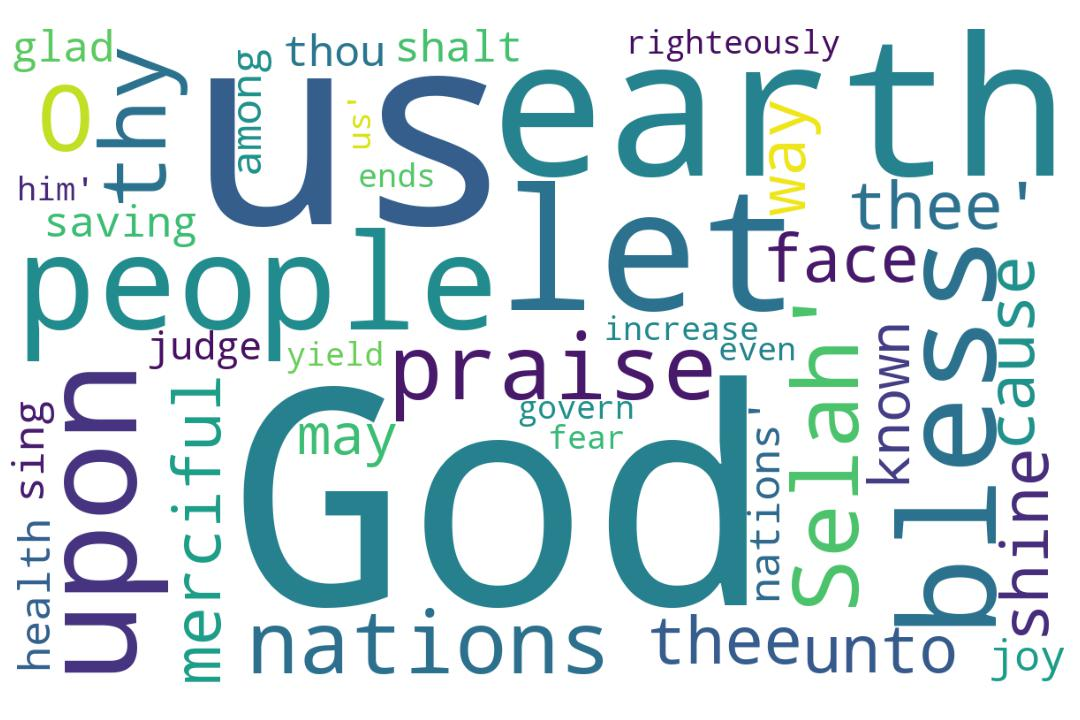
\includegraphics[width=\linewidth]{19OT-Psalms/Psalm67-WordCloud.jpg}
  \caption{Psalm 67 Word Cloud}
  \label{fig:Psalm 67 word Cloud}
\end{figure}


\marginpar{\scriptsize \centering \fcolorbox{bone}{lime}{\textbf{A PLEA FOR MERCY}}\\ (Psalm 67:1-7) \begin{compactenum}[I.][8]
    \item The \textbf{Cause of Comfort} \index[scripture]{Psalms!Psa 067:01}(Psa 67:1)
    \item A \textbf{Corporate Concern} \index[scripture]{Psalms!Psa 067:02}(Psa 67:2)
    \item A \textbf{Common Chorus} \index[scripture]{Psalms!Psa 067:04}(Psa 67:4)
    \item A \textbf{Cure for the Curse} \index[scripture]{Psalms!Psa 067:06}(Psa 67:6)
    \item A \textbf{Comforting Conclusion} \index[scripture]{Psalms!Psa 067:07}(Psa 67:7)
\end{compactenum}}

\footnote{\textcolor[rgb]{0.00,0.25,0.00}{\hyperlink{TOC}{Return to end of Table of Contents.}}}\footnote{\href{https://audiobible.com/bible/psalms_67.html}{\textcolor[cmyk]{0.99998,1,0,0}{Psalm 67 Audio}}}\textcolor[cmyk]{0.99998,1,0,0}{To the chief Musician on Neginoth, A Psalm \emph{or} Song.}\\
\\
\P  \textcolor[cmyk]{0.99998,1,0,0}{God be merciful unto us, and bless us; \emph{and} cause \fcolorbox{bone}{lime}{his face to shine} upon us; Selah.}\footnote{\textbf{Numbers 6:22-27} - And the LORD spake unto Moses, saying, [23] Speak unto Aaron and unto his sons, saying, On this wise ye shall bless the children of Israel, saying unto them, [24] The LORD bless thee, and keep thee: [25] The LORD make his face shine upon thee, and be gracious unto thee: [26] The LORD lift up his countenance upon thee, and give thee peace. [27] And they shall put my name upon the children of Israel; and I will bless them.}%\footnote{The key word to orient the reader shows up twice in seven verses (``Selah'' in verses 1 and 4). By now you know what the ``majority of conservative scholars'' are going to do with it. The entire Psalm deals with the Millennium and the Millennial Reign of the Son of God (see Psalm 2, 110; Isaiah 2, 11, etc.). ``God be merciful unto us and bless us...upon us.'' Verse 1 is a prayer for the restoration of Israel. Note especially the mid-Tribulation (or end-Tribulation) appearance of the Lord from heaven, as in the case of Job (Job 38:1), Saul (Acts 9:4--7), Daniel (Daniel 10:5--11), and Ezekiel (Ezekiel 1:1--4). We have commented on this under Psalm 31:16, which Kroll, Motyer, Yates, Jamieson, Baethgen, Briggs, Ewald, Dummelow, and Hengstenberg went by like they were in the Indianapolis 500. ``Thy saving health'' (vs. 2) is literal (see Psalm 91:3) and extends into eternity for the ``nations'' (see Revelation 22:2). ``All the people praise'' Him (see Psalm 2 and 110), and the ``nations'' will be glad and sing for joy, for the ``fulness of Israel'' (Romans 11:12) will affect nature (see Romans 8:20--27; Isaiah 11:1--10; Amos 9:13, etc.). The characteristics of the Millennium are Joy (vs. 4), Gladness (vs. 4), Blessing (vss. 1--7), Singing (vs. 4), Mercy (vs. 1), Praise (vs. 3), Righteousness (vs. 4), and Increase (vs. 6). This is the “Golden Age” of the unsaved philosophers; the “Thousand Year Reich” of the Nazis; the “Camelot” of the depraved Kennedy family; the “Great Society” of Lyndon Johnson, and the infamous “bringing in of Thy Kingdom” the Southern Baptists wasted their time on. It is the “Our Father” of the pagan Catholics answered at last—“thy kingdom come”— after those depraved killers had been praying it for sixteen hundred years. It came about without their help and despite their efforts, and when it came it destroyed their church, their theology, their priests and nuns, bishops and cardinals, archbishops and popes in one lick, because it was a Jewish kingdom (Luke 1:32). “Salvation is of the Jews” (John 4:22). Rome was never given the privilege, at either Advent, of saving anyone. \cite{Ruckman1992Psalms} }
[2] \textcolor[cmyk]{0.99998,1,0,0}{That thy way may be known upon earth, thy saving health \fcolorbox{bone}{lime}{among all nations}.} %\footnote{Ready for chaos? Here it is: ``May the people praise you...for you rule [present tense] the people justly'' (verses 3--4). This is the aborted perversion known as the New International Version. It simply erased the Millennial references. The nation’s knowledge of God is not even conditioned on God blessing Israel in the NIV, for the words “That thy way may be known” (vs. 2) have been removed from it. This is the godless abomination that bragged about how much more “readable” it was than the King James Bible and proved it by testing it out with a couple of hundred dead orthodox apostate kiddy school readers attached to dead orthodox churches. Not even the RSV of the NCC was this corrupt, although The Living Bible was; it did the same thing in order to disconnect the knowledge of God by the nations with the coming of the Lord. The Living Bible even destroys the sense of verse 1 by making it a present tense: ``as you look down on us.'' Kyle Yates (RSV committee) tells us that the Psalm is “Remarkable for its beauty, its simplicity and its world outlook.” (Can’t you guess what he is going to do? You get one guess!) “God’s gracious dealings are viewed as the means by which all people are led to turn to God...this is a striking universalistic note...expressing hope for God’s continued blessing in order that Israel’s mission may be completed.” \cite{Ruckman1992Psalms}} 
[3] \textcolor[cmyk]{0.99998,1,0,0}{Let the people praise thee, O God; let all the people praise thee.}
[4] \textcolor[cmyk]{0.99998,1,0,0}{O let the nations be glad and \fcolorbox{bone}{lime}{sing for joy}: for thou shalt judge the people righteously, and govern the nations upon earth. Selah.} %\footnote{Interpretation? “Rapunzel, Rapunzel, let down your golden hair.” No Advent, no return of Christ, no throne at Jerusalem, no Jesus Christ, no scriptural fulfillment, no restoration of Israel: just one big, godless, hellish, damnable denial of the main theme of the Bible, laden with enough piety and “godliness” to “gag a maggot” (circa 1980, Middle Schools). Kroll, being Premillennial, is finally forced to show his hand at verse 4, but not till then. He disassociates verse 1 from the Tribulation and the Advent and does away with the “saving health” by saying contemptuously it is “to be understood in the singular sense as salvation among all nations.” He didn’t make any connection with “health” at all, as it was given in Psalm 91:3; Ezekiel chapter 47; and Revelation 22:2; he equated “health” with Church Age salvation. Poor old Dummelow splashes around like a crippled thrasher in a bird bath. He wants the RV reading of Westcott and Hort put back into verses 4 and 6 and says that “God’s goodness to Israel reveals him [present tense] to the nations,” which of course is more nonsense. But Jamieson and Brown have the best way of saying what you don’t mean so you will think they mean what they think they didn’t say: “The manifest blessedness of Israel IN HER LORD shall attract all nations to the same Saviour...when all the people praise God then the earth itself shall be delivered from the curse...the future is to the eye of inspiration as sure as the already past...God’s blessing on the literal and spiritual Israel shall be the FORERUNNER of the conversion of the world.” Beautiful, ain’t it? No date given, no Lord returning, no Lord landing, no Lord reigning, no judgment on the nations, no judging the nations literally on earth, and no renovation of nature because of the King’s presence. The “blessing” came from people praising God. Dale Carnegie, Chuck Swindoll, Robert Schuller, and Norman Vincent Peale never did it any better. This is a typical masterpiece of “toning down,” “leavening,” and “stripping” a passage of its Biblical content. It is a dehydrating, blood letting, artificial preservative type of exposition that fills the works of the “godly scholars.” In the raw it is simply two things: unbelief and cowardice. \cite{Ruckman1992Psalms} }
[5] \textcolor[cmyk]{0.99998,1,0,0}{Let the people praise thee, O God; let all the people praise thee.}
[6] \textcolor[cmyk]{0.99998,1,0,0}{\emph{Then} shall the earth yield her increase; \emph{and} God, \emph{even} our own God, \fcolorbox{bone}{lime}{shall bless us}.}
[7] \textcolor[cmyk]{0.99998,1,0,0}{God shall bless us; and all the \fcolorbox{bone}{lime}{ends of the earth} shall fear him.}
\index[NWIV]{17!Psalms!Psa 67:1}\index[AWIP]{God!Psalms!Psa 67:1}\index[AWIP]{be!Psalms!Psa 67:1}\index[AWIP]{merciful!Psalms!Psa 67:1}\index[AWIP]{unto!Psalms!Psa 67:1}\index[AWIP]{us!Psalms!Psa 67:1}\index[AWIP]{us!Psalms!Psa 67:1 (2)}\index[AWIP]{us!Psalms!Psa 67:1 (3)}\index[AWIP]{and!Psalms!Psa 67:1}\index[AWIP]{bless!Psalms!Psa 67:1}\index[AWIP]{\emph{and}!Psalms!Psa 67:1}\index[AWIP]{cause!Psalms!Psa 67:1}\index[AWIP]{his!Psalms!Psa 67:1}\index[AWIP]{face!Psalms!Psa 67:1}\index[AWIP]{to!Psalms!Psa 67:1}\index[AWIP]{shine!Psalms!Psa 67:1}\index[AWIP]{upon!Psalms!Psa 67:1}\index[AWIP]{Selah!Psalms!Psa 67:1}\index[AWIP]{\emph{and}!Psalms!Psa 67:1}

\index[NWIV]{14!Psalms!Psa 67:2}\index[AWIP]{That!Psalms!Psa 67:2}\index[AWIP]{thy!Psalms!Psa 67:2}\index[AWIP]{thy!Psalms!Psa 67:2 (2)}\index[AWIP]{way!Psalms!Psa 67:2}\index[AWIP]{may!Psalms!Psa 67:2}\index[AWIP]{be!Psalms!Psa 67:2}\index[AWIP]{known!Psalms!Psa 67:2}\index[AWIP]{upon!Psalms!Psa 67:2}\index[AWIP]{earth!Psalms!Psa 67:2}\index[AWIP]{saving!Psalms!Psa 67:2}\index[AWIP]{health!Psalms!Psa 67:2}\index[AWIP]{among!Psalms!Psa 67:2}\index[AWIP]{all!Psalms!Psa 67:2}\index[AWIP]{nations!Psalms!Psa 67:2}

\index[NWIV]{13!Psalms!Psa 67:3}\index[AWIP]{Let!Psalms!Psa 67:3}\index[AWIP]{the!Psalms!Psa 67:3}\index[AWIP]{the!Psalms!Psa 67:3 (2)}\index[AWIP]{people!Psalms!Psa 67:3}\index[AWIP]{people!Psalms!Psa 67:3 (2)}\index[AWIP]{praise!Psalms!Psa 67:3}\index[AWIP]{praise!Psalms!Psa 67:3 (2)}\index[AWIP]{thee!Psalms!Psa 67:3}\index[AWIP]{thee!Psalms!Psa 67:3 (2)}\index[AWIP]{O!Psalms!Psa 67:3}\index[AWIP]{God!Psalms!Psa 67:3}\index[AWIP]{let!Psalms!Psa 67:3}\index[AWIP]{all!Psalms!Psa 67:3}

\index[NWIV]{24!Psalms!Psa 67:4}\index[AWIP]{O!Psalms!Psa 67:4}\index[AWIP]{let!Psalms!Psa 67:4}\index[AWIP]{the!Psalms!Psa 67:4}\index[AWIP]{the!Psalms!Psa 67:4 (2)}\index[AWIP]{the!Psalms!Psa 67:4 (3)}\index[AWIP]{nations!Psalms!Psa 67:4}\index[AWIP]{nations!Psalms!Psa 67:4 (2)}\index[AWIP]{be!Psalms!Psa 67:4}\index[AWIP]{glad!Psalms!Psa 67:4}\index[AWIP]{and!Psalms!Psa 67:4}\index[AWIP]{and!Psalms!Psa 67:4 (2)}\index[AWIP]{sing!Psalms!Psa 67:4}\index[AWIP]{for!Psalms!Psa 67:4}\index[AWIP]{for!Psalms!Psa 67:4 (2)}\index[AWIP]{joy!Psalms!Psa 67:4}\index[AWIP]{thou!Psalms!Psa 67:4}\index[AWIP]{shalt!Psalms!Psa 67:4}\index[AWIP]{judge!Psalms!Psa 67:4}\index[AWIP]{people!Psalms!Psa 67:4}\index[AWIP]{righteously!Psalms!Psa 67:4}\index[AWIP]{govern!Psalms!Psa 67:4}\index[AWIP]{upon!Psalms!Psa 67:4}\index[AWIP]{earth!Psalms!Psa 67:4}\index[AWIP]{Selah!Psalms!Psa 67:4}

\index[NWIV]{13!Psalms!Psa 67:5}\index[AWIP]{Let!Psalms!Psa 67:5}\index[AWIP]{the!Psalms!Psa 67:5}\index[AWIP]{the!Psalms!Psa 67:5 (2)}\index[AWIP]{people!Psalms!Psa 67:5}\index[AWIP]{people!Psalms!Psa 67:5 (2)}\index[AWIP]{praise!Psalms!Psa 67:5}\index[AWIP]{praise!Psalms!Psa 67:5 (2)}\index[AWIP]{thee!Psalms!Psa 67:5}\index[AWIP]{thee!Psalms!Psa 67:5 (2)}\index[AWIP]{O!Psalms!Psa 67:5}\index[AWIP]{God!Psalms!Psa 67:5}\index[AWIP]{let!Psalms!Psa 67:5}\index[AWIP]{all!Psalms!Psa 67:5}

\index[NWIV]{16!Psalms!Psa 67:6}\index[AWIP]{\emph{Then}!Psalms!Psa 67:6}\index[AWIP]{shall!Psalms!Psa 67:6}\index[AWIP]{shall!Psalms!Psa 67:6 (2)}\index[AWIP]{the!Psalms!Psa 67:6}\index[AWIP]{earth!Psalms!Psa 67:6}\index[AWIP]{yield!Psalms!Psa 67:6}\index[AWIP]{her!Psalms!Psa 67:6}\index[AWIP]{increase!Psalms!Psa 67:6}\index[AWIP]{\emph{and}!Psalms!Psa 67:6}\index[AWIP]{God!Psalms!Psa 67:6}\index[AWIP]{God!Psalms!Psa 67:6 (2)}\index[AWIP]{\emph{even}!Psalms!Psa 67:6}\index[AWIP]{our!Psalms!Psa 67:6}\index[AWIP]{own!Psalms!Psa 67:6}\index[AWIP]{bless!Psalms!Psa 67:6}\index[AWIP]{us!Psalms!Psa 67:6}\index[AWIP]{\emph{Then}!Psalms!Psa 67:6}\index[AWIP]{\emph{and}!Psalms!Psa 67:6}\index[AWIP]{\emph{even}!Psalms!Psa 67:6}

\index[NWIV]{14!Psalms!Psa 67:7}\index[AWIP]{God!Psalms!Psa 67:7}\index[AWIP]{shall!Psalms!Psa 67:7}\index[AWIP]{shall!Psalms!Psa 67:7 (2)}\index[AWIP]{bless!Psalms!Psa 67:7}\index[AWIP]{us!Psalms!Psa 67:7}\index[AWIP]{and!Psalms!Psa 67:7}\index[AWIP]{all!Psalms!Psa 67:7}\index[AWIP]{the!Psalms!Psa 67:7}\index[AWIP]{the!Psalms!Psa 67:7 (2)}\index[AWIP]{ends!Psalms!Psa 67:7}\index[AWIP]{of!Psalms!Psa 67:7}\index[AWIP]{earth!Psalms!Psa 67:7}\index[AWIP]{fear!Psalms!Psa 67:7}\index[AWIP]{him!Psalms!Psa 67:7}


\section{Psalm 67 Outlines}

\subsection{My Outlines}

\subsubsection{A Plea for Mercy}
\index[speaker]{Keith Anthony!Psalm 067 (A Plea for Mercy)}
\index[series]{Psalms (Keith Anthony)!Psalm 067 (A Plea for Mercy)}
\index[date]{2017/08/11!Psalm 067 (A Plea for Mercy) (Keith Anthony)}

\begin{compactenum}[I.]
    \item The \textbf{Cause of Comfort} \index[scripture]{Psalms!Psa 067:01}(Psa 67:1)
    \item A \textbf{Corporate Concern} \index[scripture]{Psalms!Psa 067:02}(Psa 67:2)
    \item A \textbf{Common Chorus} \index[scripture]{Psalms!Psa 067:04}(Psa 67:4)
    \item A \textbf{Cure for the Curse} \index[scripture]{Psalms!Psa 067:06}(Psa 67:6)
    \item A \textbf{Comforting Conclusion} \index[scripture]{Psalms!Psa 067:07}(Psa 67:7)
\end{compactenum}






\subsection{Outlines from Others}


\section{Psalm 67 Comments}

\subsection{Numeric Nuggets}
Verses 3 and 5 have 13 words. Verse 2 has 13 unique words.
\newpage
\subsection{Psalm 67 Repeated Phrases}


%%%%%%%%%%
%%%%%%%%%%
\normalsize
 
\begin{center}
\begin{longtable}{|p{3.0in}|p{0.5in}|}
\caption[Psalm 67 Repeated Phrases]{Psalm 67 Repeated Phrases}\label{table:Repeated Phrases Psalm 67} \\
\hline \multicolumn{1}{|c|}{\textbf{Phrase}} & \multicolumn{1}{c|}{\textbf{Frequency}} \\ \hline 
\endfirsthead
 
\multicolumn{2}{c}
{{\bfseries \tablename\ \thetable{} -- continued from previous page}} \\  
\hline \multicolumn{1}{|c|}{\textbf{Phrase}} & \multicolumn{1}{c|}{\textbf{Frequency}} \\ \hline 
\endhead
 
\hline \multicolumn{2}{c}{{ }} \\ \hline
\endfoot 
the people & 5\\ \hline 
the people praise & 4\\ \hline 
the people praise thee & 4\\ \hline 
people praise & 4\\ \hline 
people praise thee & 4\\ \hline 
praise thee & 4\\ \hline 
bless us & 3\\ \hline 
all the & 3\\ \hline 
\end{longtable}
\end{center}



%%%%%%%%%%
%%%%%%%%%%



\section{Psalm 67 Statistics}

%%%%%%%%%%%%%%%%%%%%%%%%%%%
%%%%% Word Statistics
%%%%%%%%%%%%%%%%%%%%%%%%%%


\normalsize



\subsection{Chapter Word Statistics}


%%%%%%%%%%
%%%%%%%%%%
 
\begin{center}
\begin{longtable}{l|c|c|c|c}
\caption[Stats for Psalm 67]{Stats for Psalm 67} \label{table:Stats for Psalm 67} \\ 
\hline \multicolumn{1}{|c|}{\textbf{Verse(s)}} & \multicolumn{1}{|c|}{\textbf{Count}} & \multicolumn{1}{|c|}{\textbf{Unique}} & \multicolumn{1}{|c|}{\textbf{Italics}} & \multicolumn{1}{|c|}{\textbf{Uniq Italic}}  \\ \hline 
\endfirsthead
 
\multicolumn{5}{c}
{{\bfseries \tablename\ \thetable{} -- continued from previous page}} \\  
\hline \multicolumn{1}{|c|}{\textbf{Verse(s)}} & \multicolumn{1}{|c|}{\textbf{Count}} & \multicolumn{1}{|c|}{\textbf{Unique}} & \multicolumn{1}{|c|}{\textbf{Italics}} & \multicolumn{1}{|c|}{\textbf{Uniq Italic}}  \\ \hline 
\endhead
 
\hline \multicolumn{5}{|r|}{{Continued if needed}} \\ \hline
\endfoot 
1 & 17 & 15 & 1 & 1\\ \hline
2 & 14 & 13 & 0 & 0\\ \hline
3 & 13 & 9 & 0 & 0\\ \hline
4 & 24 & 19 & 0 & 0\\ \hline
5 & 13 & 9 & 0 & 0\\ \hline
6 & 16 & 14 & 3 & 3\\ \hline
7 & 14 & 12 & 0 & 0\\ \hline
\hline \hline
Total & 111 & 54 & 4 & 3



\end{longtable}
\end{center}

%%%%%%%%%%
%%%%%%%%%%
 
\subsection{Words by Frequency}

\begin{center}
\begin{longtable}{l|r}
\caption[Word Frequencies in Psalm 67]{Word Frequencies in Psalm 67} \label{table:WordsIn-Psalm-67} \\ 
\hline \multicolumn{1}{|c|}{\textbf{Word}} & \multicolumn{1}{c|}{\textbf{Frequency}} \\ \hline 
\endfirsthead
 
\multicolumn{2}{c}
{{\bfseries \tablename\ \thetable{} -- continued from previous page}} \\ 
\hline \multicolumn{1}{|c|}{\textbf{Word}} & \multicolumn{1}{c|}{\textbf{Frequency}} \\ \hline 
\endhead
 
\hline \multicolumn{2}{|r|}{{Continued if needed}} \\ \hline
\endfoot
 
\hline \hline
\endlastfoot
the & 10 \\ \hline
God & 6 \\ \hline
us & 5 \\ \hline
people & 5 \\ \hline
and & 4 \\ \hline
earth & 4 \\ \hline
all & 4 \\ \hline
praise & 4 \\ \hline
thee & 4 \\ \hline
shall & 4 \\ \hline
be & 3 \\ \hline
bless & 3 \\ \hline
upon & 3 \\ \hline
nations & 3 \\ \hline
O & 3 \\ \hline
let & 3 \\ \hline
\emph{and} & 2 \\ \hline
Selah & 2 \\ \hline
thy & 2 \\ \hline
Let & 2 \\ \hline
for & 2 \\ \hline
merciful & 1 \\ \hline
unto & 1 \\ \hline
cause & 1 \\ \hline
his & 1 \\ \hline
face & 1 \\ \hline
to & 1 \\ \hline
shine & 1 \\ \hline
That & 1 \\ \hline
way & 1 \\ \hline
may & 1 \\ \hline
known & 1 \\ \hline
saving & 1 \\ \hline
health & 1 \\ \hline
among & 1 \\ \hline
glad & 1 \\ \hline
sing & 1 \\ \hline
joy & 1 \\ \hline
thou & 1 \\ \hline
shalt & 1 \\ \hline
judge & 1 \\ \hline
righteously & 1 \\ \hline
govern & 1 \\ \hline
\emph{Then} & 1 \\ \hline
yield & 1 \\ \hline
her & 1 \\ \hline
increase & 1 \\ \hline
\emph{even} & 1 \\ \hline
our & 1 \\ \hline
own & 1 \\ \hline
ends & 1 \\ \hline
of & 1 \\ \hline
fear & 1 \\ \hline
him & 1 \\ \hline
\end{longtable}
\end{center}



\normalsize



\subsection{Words Alphabetically}

\begin{center}
\begin{longtable}{l|r}
\caption[Word Alphabetically in Psalm 67]{Word Alphabetically in Psalm 67} \label{table:WordsIn-Psalm-67} \\ 
\hline \multicolumn{1}{|c|}{\textbf{Word}} & \multicolumn{1}{c|}{\textbf{Frequency}} \\ \hline 
\endfirsthead
 
\multicolumn{2}{c}
{{\bfseries \tablename\ \thetable{} -- continued from previous page}} \\ 
\hline \multicolumn{1}{|c|}{\textbf{Word}} & \multicolumn{1}{c|}{\textbf{Frequency}} \\ \hline 
\endhead
 
\hline \multicolumn{2}{|r|}{{Continued if needed}} \\ \hline
\endfoot
 
\hline \hline
\endlastfoot
God & 6 \\ \hline
Let & 2 \\ \hline
O & 3 \\ \hline
Selah & 2 \\ \hline
That & 1 \\ \hline
\emph{Then} & 1 \\ \hline
\emph{and} & 2 \\ \hline
\emph{even} & 1 \\ \hline
all & 4 \\ \hline
among & 1 \\ \hline
and & 4 \\ \hline
be & 3 \\ \hline
bless & 3 \\ \hline
cause & 1 \\ \hline
earth & 4 \\ \hline
ends & 1 \\ \hline
face & 1 \\ \hline
fear & 1 \\ \hline
for & 2 \\ \hline
glad & 1 \\ \hline
govern & 1 \\ \hline
health & 1 \\ \hline
her & 1 \\ \hline
him & 1 \\ \hline
his & 1 \\ \hline
increase & 1 \\ \hline
joy & 1 \\ \hline
judge & 1 \\ \hline
known & 1 \\ \hline
let & 3 \\ \hline
may & 1 \\ \hline
merciful & 1 \\ \hline
nations & 3 \\ \hline
of & 1 \\ \hline
our & 1 \\ \hline
own & 1 \\ \hline
people & 5 \\ \hline
praise & 4 \\ \hline
righteously & 1 \\ \hline
saving & 1 \\ \hline
shall & 4 \\ \hline
shalt & 1 \\ \hline
shine & 1 \\ \hline
sing & 1 \\ \hline
the & 10 \\ \hline
thee & 4 \\ \hline
thou & 1 \\ \hline
thy & 2 \\ \hline
to & 1 \\ \hline
unto & 1 \\ \hline
upon & 3 \\ \hline
us & 5 \\ \hline
way & 1 \\ \hline
yield & 1 \\ \hline
\end{longtable}
\end{center}



\normalsize



\subsection{Word Lengths in Chapter}
\normalsize
\begin{longtable}{l|p{3.75in}}
\caption[Words by Length in Psalm 67]{Words by Length in Psalm 67} \label{table:WordsIn-Psalm-67} \\ 
\hline \multicolumn{1}{|c|}{\textbf{Length}} & \multicolumn{1}{c|}{\textbf{Words}} \\ \hline 
\endfirsthead
 
\multicolumn{2}{c}
{{\bfseries \tablename\ \thetable{} -- continued from previous page}} \\ 
\hline \multicolumn{1}{|c|}{\textbf{Length}} & \multicolumn{1}{c|}{\textbf{Words}} \\ \hline 
\endhead
 
\hline \multicolumn{2}{|r|}{{Continued if needed}} \\ \hline
\endfoot
 
\hline \hline
\endlastfoot
1 & O \\ \hline
2 & be, us, to, of \\ \hline
3 & God, and, \emph{and}, his, thy, way, may, all, Let, the, let, for, joy, her, our, own, him \\ \hline
4 & unto, face, upon, That, thee, glad, sing, thou, \emph{Then}, \emph{even}, ends, fear \\ \hline
5 & bless, cause, shine, Selah, known, earth, among, shalt, judge, shall, yield \\ \hline
6 & saving, health, people, praise, govern \\ \hline
7 & nations \\ \hline
8 & merciful, increase \\ \hline
11 & righteously \\ \hline
\end{longtable}






%%%%%%%%%%
%%%%%%%%%%
 



%%%%%%%%%%
%%%%%%%%%%
\subsection{Verses with 13 Words in Chapter}
\normalsize
\begin{longtable}{l|p{3.75in}}
\caption[Verses with 13 Words  in Psalm 67]{Verses with 13 Words  in Psalm 67} \label{table:Verses with 13 Words in-Psalm-67} \\ 
\hline \multicolumn{1}{|c|}{\textbf{Reference}} & \multicolumn{1}{c|}{\textbf{Verse}} \\ \hline 
\endfirsthead
 
\multicolumn{2}{c}
{{\bfseries \tablename\ \thetable{} -- continued from previous page}} \\ 
\hline \multicolumn{1}{|c|}{\textbf{Reference}} & \multicolumn{1}{c|}{\textbf{Verse}} \\ \hline 
\endhead
 
\hline \multicolumn{2}{|r|}{{Continued if needed}} \\ \hline
\endfoot
 
\hline \hline
\endlastfoot
Psalms 067:3 & Let the people praise thee, O God; let all the people praise thee. \\ \hline
Psalms 067:5 & Let the people praise thee, O God; let all the people praise thee. \\ \hline
\end{longtable}






%%%%%%%%%%
%%%%%%%%%%

\chapter{Proverb 9}

\begin{figure}
  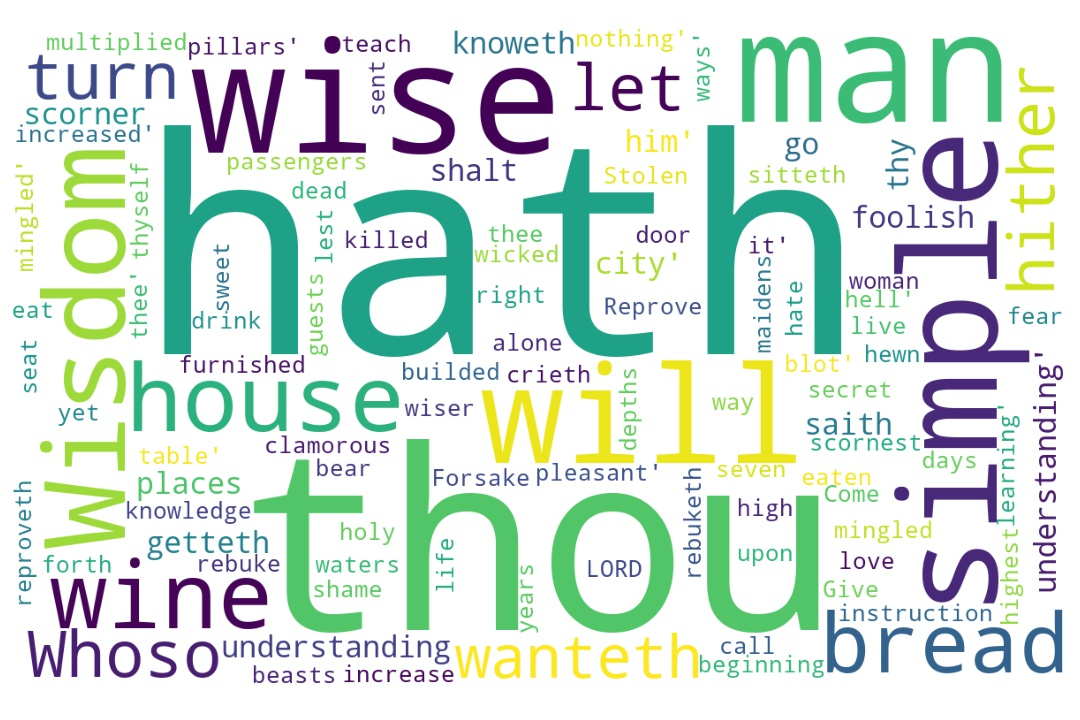
\includegraphics[width=\linewidth]{20OT-Proverbs/Proverb9-WordCloud.jpg}
  \caption{Proverb 9 Word Cloud}
  \label{fig:Proverb 9 Word Cloud}
\end{figure}


\marginpar{\scriptsize \centering \fcolorbox{bone}{lime}{\textbf{WISDOM: THE GOOD CHOICE}}\\ (Proverb 9:1-18) \begin{compactenum}[I.][8]
\item \textbf{Builds} a Life \index[scripture]{Proverbs!Pro 09:01}(Pro 9:1)
\item Has a \textbf{Banquet} \index[scripture]{Proverbs!Pro 09:02}(Pro 9:2)
\item Gives out \textbf{Bread} \index[scripture]{Proverbs!Pro 09:05}(Pro 9:5)
\item Has \textbf{Blessings} \index[scripture]{Proverbs!Pro 09:09}(Pro 9:9)
\item Was there from the \textbf{Beginning} \index[scripture]{Proverbs!Pro 09:10}(Pro 9:10)
\item Provides Lasting \textbf{Benefits} \index[scripture]{Proverbs!Pro 09:11}(Pro 9:11)
\item Is \textbf{Betrayed} \index[scripture]{Proverbs!Pro 09:13}(Pro 9:13)
\end{compactenum}}

\marginpar{\scriptsize \centering \fcolorbox{bone}{yellow}{\textbf{WISDOM AT WORK}}\\ (Proverb 9:1-18) \begin{compactenum}[I.][8]
    \item \textbf{Builds a House} \index[scripture]{Proverbs!Pro 09:01}(Pro 9:1)
    \item \textbf{Hews out Pillars} \index[scripture]{Proverbs!Pro 09:01}(Pro 9:1)
    \item \textbf{Kills her Beats} \index[scripture]{Proverbs!Pro 09:02}(Pro 9:2)
    \item \textbf{Mingles Her Wine} \index[scripture]{Proverbs!Pro 09:02}(Pro 9:2)
    \item \textbf{Furnishes her Table} \index[scripture]{Proverbs!Pro 09:02}(Pro 9:2)
    \item \textbf{Sends forthe her Maidens} \index[scripture]{Proverbs!Pro 09:03}(Pro 9:3)
    \item \textbf{Cries from the High Places} \index[scripture]{Proverbs!Pro 09:03}(Pro 9:3)
\end{compactenum}}

\marginpar{\scriptsize \centering \fcolorbox{bone}{black}{\textbf{\textcolor[cmyk]{0,0,0,0}{LOOKING FOR WISDOM}}}\\ (Proverb 9) 
\begin{compactenum}[I.][8]
    \item The \textbf{Rendering of Wisdom} \index[scripture]{Proverbs!Pro 09:01}(Pro 9:1) 
   \item The \textbf{Reaction to Wisdom} \index[scripture]{Proverbs!Pro 09:09}(Pro 9:9) 
    \item The \textbf{Reach for Wisdom} \index[scripture]{Proverbs!Pro 09:10}(Pro 9:10) 
    \item The \textbf{Road to Wisdom} \index[scripture]{Proverbs!Pro 09:11}(Pro 9:11) 
    \item The \textbf{Rejection of Wisdom} \index[scripture]{Proverbs!Pro 09:13}(Pro 9:13) 
    \item Man's \textbf{Regard \& Reverence for Foolishness} \index[scripture]{Proverbs!Pro 09:14}(Pro 9:14) 
    \item A \textbf{Reunion of Fools} \index[scripture]{Proverbs!Pro 09:15}(Pro 9:15) 
\end{compactenum}}

\footnote{\textcolor[cmyk]{0.99998,1,0,0}{\hyperlink{TOC}{Return to end of Table of Contents.}}}\footnote{\href{https://audiobible.com/bible/proverbs_9.html}{\textcolor[cmyk]{0.99998,1,0,0}{Proverbs Audio}}}\textcolor[cmyk]{0.99998,1,0,0}{Wisdom hath \fcolorbox{bone}{lime}{builded her house}, she hath hewn out her seven pillars:}\footnote{\textbf{1 Kings 8:27} - But will God indeed dwell on the earth? behold, the heaven and heaven of heavens cannot contain thee; how much less this house that I have builded?} 
[2] \textcolor[cmyk]{0.99998,1,0,0}{She hath killed her beasts; she hath mingled her wine; she hath also \fcolorbox{bone}{lime}{furnished} her table.}
[3] \textcolor[cmyk]{0.99998,1,0,0}{She hath sent forth her maidens: she crieth upon the highest places of the city,}
[4] \textcolor[cmyk]{0.99998,1,0,0}{Whoso \emph{is} simple, let him turn in hither: \emph{as} \emph{for} him that wanteth \fcolorbox{bone}{MYGOLD}{understanding}, she saith to him,}
[5] \textcolor[cmyk]{0.99998,1,0,0}{Come, \fcolorbox{bone}{lime}{eat of my} \fcolorbox{bone}{lime}{bread}, and drink of the wine \emph{which} I have mingled.}
[6] \textcolor[cmyk]{0.99998,1,0,0}{Forsake the foolish, and live; and go in the way of \fcolorbox{bone}{MYGOLD}{understanding}.}
[7] \textcolor[cmyk]{0.99998,1,0,0}{He that reproveth a scorner getteth to himself shame: and he that rebuketh a wicked \emph{man} \emph{getteth} himself a blot.}
[8] \textcolor[cmyk]{0.99998,1,0,0}{Reprove not a scorner, lest he hate thee: rebuke a wise man, and he will love thee.}
[9] \textcolor[cmyk]{0.99998,1,0,0}{Give \emph{instruction} to a wise \emph{man}, and he will \fcolorbox{bone}{lime}{be yet wiser}: teach a just \emph{man}, and he will increase in learning.}
[10] \textcolor[cmyk]{0.99998,1,0,0}{The fear of the LORD \emph{is} the \fcolorbox{bone}{lime}{beginning of wisdom}: and the knowledge of the holy \emph{is} \fcolorbox{bone}{MYGOLD}{understanding}.}
[11] \textcolor[cmyk]{0.99998,1,0,0}{For by me thy days shall be multiplied, and the years of thy life shall be \fcolorbox{bone}{lime}{increased}.}
[12] \textcolor[cmyk]{0.99998,1,0,0}{If thou be wise, thou shalt be wise for thyself: but \emph{if} thou scornest, thou alone shalt bear \emph{it}.}
[13] \textcolor[cmyk]{0.99998,1,0,0}{A foolish woman \emph{is} clamorous: \emph{she} \emph{is} simple, and \fcolorbox{bone}{lime}{knoweth nothing}.}
[14] \textcolor[cmyk]{0.99998,1,0,0}{For she sitteth at the door of her house, on a seat in the high places of the city,}
[15] \textcolor[cmyk]{0.99998,1,0,0}{To call passengers who go right on their ways:}
[16] \textcolor[cmyk]{0.99998,1,0,0}{Whoso \emph{is} simple, let him turn in hither: and \emph{as} \emph{for} him that wanteth \fcolorbox{bone}{MYGOLD}{understanding}, she saith to him,}
[17] \textcolor[cmyk]{0.99998,1,0,0}{Stolen waters are sweet, and bread \emph{eaten} in secret is pleasant.}
[18] \textcolor[cmyk]{0.99998,1,0,0}{But he knoweth not that the dead \emph{are} there; \emph{and} \emph{that} her guests \emph{are} in the depths of hell.}



\index[NWIV]{12!Proverbs!Pro 9:1}\index[AWIP]{Wisdom!Proverbs!Pro 9:1}\index[AWIP]{hath!Proverbs!Pro 9:1}\index[AWIP]{hath!Proverbs!Pro 9:1 (2)}\index[AWIP]{builded!Proverbs!Pro 9:1}\index[AWIP]{her!Proverbs!Pro 9:1}\index[AWIP]{her!Proverbs!Pro 9:1 (2)}\index[AWIP]{house!Proverbs!Pro 9:1}\index[AWIP]{she!Proverbs!Pro 9:1}\index[AWIP]{hewn!Proverbs!Pro 9:1}\index[AWIP]{out!Proverbs!Pro 9:1}\index[AWIP]{seven!Proverbs!Pro 9:1}\index[AWIP]{pillars!Proverbs!Pro 9:1}

\index[NWIV]{16!Proverbs!Pro 9:2}\index[AWIP]{She!Proverbs!Pro 9:2}\index[AWIP]{hath!Proverbs!Pro 9:2}\index[AWIP]{hath!Proverbs!Pro 9:2 (2)}\index[AWIP]{hath!Proverbs!Pro 9:2 (3)}\index[AWIP]{killed!Proverbs!Pro 9:2}\index[AWIP]{her!Proverbs!Pro 9:2}\index[AWIP]{her!Proverbs!Pro 9:2 (2)}\index[AWIP]{her!Proverbs!Pro 9:2 (3)}\index[AWIP]{beasts!Proverbs!Pro 9:2}\index[AWIP]{she!Proverbs!Pro 9:2}\index[AWIP]{she!Proverbs!Pro 9:2 (2)}\index[AWIP]{mingled!Proverbs!Pro 9:2}\index[AWIP]{wine!Proverbs!Pro 9:2}\index[AWIP]{also!Proverbs!Pro 9:2}\index[AWIP]{furnished!Proverbs!Pro 9:2}\index[AWIP]{table!Proverbs!Pro 9:2}

\index[NWIV]{15!Proverbs!Pro 9:3}\index[AWIP]{She!Proverbs!Pro 9:3}\index[AWIP]{hath!Proverbs!Pro 9:3}\index[AWIP]{sent!Proverbs!Pro 9:3}\index[AWIP]{forth!Proverbs!Pro 9:3}\index[AWIP]{her!Proverbs!Pro 9:3}\index[AWIP]{maidens!Proverbs!Pro 9:3}\index[AWIP]{she!Proverbs!Pro 9:3}\index[AWIP]{crieth!Proverbs!Pro 9:3}\index[AWIP]{upon!Proverbs!Pro 9:3}\index[AWIP]{the!Proverbs!Pro 9:3}\index[AWIP]{the!Proverbs!Pro 9:3 (2)}\index[AWIP]{highest!Proverbs!Pro 9:3}\index[AWIP]{places!Proverbs!Pro 9:3}\index[AWIP]{of!Proverbs!Pro 9:3}\index[AWIP]{city!Proverbs!Pro 9:3}

\index[NWIV]{18!Proverbs!Pro 9:4}\index[AWIP]{Whoso!Proverbs!Pro 9:4}\index[AWIP]{\emph{is}!Proverbs!Pro 9:4}\index[AWIP]{simple!Proverbs!Pro 9:4}\index[AWIP]{let!Proverbs!Pro 9:4}\index[AWIP]{him!Proverbs!Pro 9:4}\index[AWIP]{him!Proverbs!Pro 9:4 (2)}\index[AWIP]{him!Proverbs!Pro 9:4 (3)}\index[AWIP]{turn!Proverbs!Pro 9:4}\index[AWIP]{in!Proverbs!Pro 9:4}\index[AWIP]{hither!Proverbs!Pro 9:4}\index[AWIP]{\emph{as}!Proverbs!Pro 9:4}\index[AWIP]{\emph{for}!Proverbs!Pro 9:4}\index[AWIP]{that!Proverbs!Pro 9:4}\index[AWIP]{wanteth!Proverbs!Pro 9:4}\index[AWIP]{understanding!Proverbs!Pro 9:4}\index[AWIP]{she!Proverbs!Pro 9:4}\index[AWIP]{saith!Proverbs!Pro 9:4}\index[AWIP]{to!Proverbs!Pro 9:4}\index[AWIP]{\emph{is}!Proverbs!Pro 9:4}\index[AWIP]{\emph{as}!Proverbs!Pro 9:4}\index[AWIP]{\emph{for}!Proverbs!Pro 9:4}

\index[NWIV]{14!Proverbs!Pro 9:5}\index[AWIP]{Come!Proverbs!Pro 9:5}\index[AWIP]{eat!Proverbs!Pro 9:5}\index[AWIP]{of!Proverbs!Pro 9:5}\index[AWIP]{of!Proverbs!Pro 9:5 (2)}\index[AWIP]{my!Proverbs!Pro 9:5}\index[AWIP]{bread!Proverbs!Pro 9:5}\index[AWIP]{and!Proverbs!Pro 9:5}\index[AWIP]{drink!Proverbs!Pro 9:5}\index[AWIP]{the!Proverbs!Pro 9:5}\index[AWIP]{wine!Proverbs!Pro 9:5}\index[AWIP]{\emph{which}!Proverbs!Pro 9:5}\index[AWIP]{I!Proverbs!Pro 9:5}\index[AWIP]{have!Proverbs!Pro 9:5}\index[AWIP]{mingled!Proverbs!Pro 9:5}\index[AWIP]{\emph{which}!Proverbs!Pro 9:5}

\index[NWIV]{12!Proverbs!Pro 9:6}\index[AWIP]{Forsake!Proverbs!Pro 9:6}\index[AWIP]{the!Proverbs!Pro 9:6}\index[AWIP]{the!Proverbs!Pro 9:6 (2)}\index[AWIP]{foolish!Proverbs!Pro 9:6}\index[AWIP]{and!Proverbs!Pro 9:6}\index[AWIP]{and!Proverbs!Pro 9:6 (2)}\index[AWIP]{live!Proverbs!Pro 9:6}\index[AWIP]{go!Proverbs!Pro 9:6}\index[AWIP]{in!Proverbs!Pro 9:6}\index[AWIP]{way!Proverbs!Pro 9:6}\index[AWIP]{of!Proverbs!Pro 9:6}\index[AWIP]{understanding!Proverbs!Pro 9:6}

\index[NWIV]{20!Proverbs!Pro 9:7}\index[AWIP]{He!Proverbs!Pro 9:7}\index[AWIP]{that!Proverbs!Pro 9:7}\index[AWIP]{that!Proverbs!Pro 9:7 (2)}\index[AWIP]{reproveth!Proverbs!Pro 9:7}\index[AWIP]{a!Proverbs!Pro 9:7}\index[AWIP]{a!Proverbs!Pro 9:7 (2)}\index[AWIP]{a!Proverbs!Pro 9:7 (3)}\index[AWIP]{scorner!Proverbs!Pro 9:7}\index[AWIP]{getteth!Proverbs!Pro 9:7}\index[AWIP]{to!Proverbs!Pro 9:7}\index[AWIP]{himself!Proverbs!Pro 9:7}\index[AWIP]{himself!Proverbs!Pro 9:7 (2)}\index[AWIP]{shame!Proverbs!Pro 9:7}\index[AWIP]{and!Proverbs!Pro 9:7}\index[AWIP]{he!Proverbs!Pro 9:7}\index[AWIP]{rebuketh!Proverbs!Pro 9:7}\index[AWIP]{wicked!Proverbs!Pro 9:7}\index[AWIP]{\emph{man}!Proverbs!Pro 9:7}\index[AWIP]{\emph{getteth}!Proverbs!Pro 9:7}\index[AWIP]{blot!Proverbs!Pro 9:7}\index[AWIP]{\emph{man}!Proverbs!Pro 9:7}\index[AWIP]{\emph{getteth}!Proverbs!Pro 9:7}

\index[NWIV]{17!Proverbs!Pro 9:8}\index[AWIP]{Reprove!Proverbs!Pro 9:8}\index[AWIP]{not!Proverbs!Pro 9:8}\index[AWIP]{a!Proverbs!Pro 9:8}\index[AWIP]{a!Proverbs!Pro 9:8 (2)}\index[AWIP]{scorner!Proverbs!Pro 9:8}\index[AWIP]{lest!Proverbs!Pro 9:8}\index[AWIP]{he!Proverbs!Pro 9:8}\index[AWIP]{he!Proverbs!Pro 9:8 (2)}\index[AWIP]{hate!Proverbs!Pro 9:8}\index[AWIP]{thee!Proverbs!Pro 9:8}\index[AWIP]{thee!Proverbs!Pro 9:8 (2)}\index[AWIP]{rebuke!Proverbs!Pro 9:8}\index[AWIP]{wise!Proverbs!Pro 9:8}\index[AWIP]{man!Proverbs!Pro 9:8}\index[AWIP]{and!Proverbs!Pro 9:8}\index[AWIP]{will!Proverbs!Pro 9:8}\index[AWIP]{love!Proverbs!Pro 9:8}

\index[NWIV]{22!Proverbs!Pro 9:9}\index[AWIP]{Give!Proverbs!Pro 9:9}\index[AWIP]{\emph{instruction}!Proverbs!Pro 9:9}\index[AWIP]{to!Proverbs!Pro 9:9}\index[AWIP]{a!Proverbs!Pro 9:9}\index[AWIP]{a!Proverbs!Pro 9:9 (2)}\index[AWIP]{wise!Proverbs!Pro 9:9}\index[AWIP]{\emph{man}!Proverbs!Pro 9:9}\index[AWIP]{\emph{man}!Proverbs!Pro 9:9 (2)}\index[AWIP]{and!Proverbs!Pro 9:9}\index[AWIP]{and!Proverbs!Pro 9:9 (2)}\index[AWIP]{he!Proverbs!Pro 9:9}\index[AWIP]{he!Proverbs!Pro 9:9 (2)}\index[AWIP]{will!Proverbs!Pro 9:9}\index[AWIP]{will!Proverbs!Pro 9:9 (2)}\index[AWIP]{be!Proverbs!Pro 9:9}\index[AWIP]{yet!Proverbs!Pro 9:9}\index[AWIP]{wiser!Proverbs!Pro 9:9}\index[AWIP]{teach!Proverbs!Pro 9:9}\index[AWIP]{just!Proverbs!Pro 9:9}\index[AWIP]{increase!Proverbs!Pro 9:9}\index[AWIP]{in!Proverbs!Pro 9:9}\index[AWIP]{learning!Proverbs!Pro 9:9}\index[AWIP]{\emph{instruction}!Proverbs!Pro 9:9}\index[AWIP]{\emph{man}!Proverbs!Pro 9:9}\index[AWIP]{\emph{man}!Proverbs!Pro 9:9 (2)}

\index[NWIV]{18!Proverbs!Pro 9:10}\index[AWIP]{The!Proverbs!Pro 9:10}\index[AWIP]{fear!Proverbs!Pro 9:10}\index[AWIP]{of!Proverbs!Pro 9:10}\index[AWIP]{of!Proverbs!Pro 9:10 (2)}\index[AWIP]{of!Proverbs!Pro 9:10 (3)}\index[AWIP]{the!Proverbs!Pro 9:10}\index[AWIP]{the!Proverbs!Pro 9:10 (2)}\index[AWIP]{the!Proverbs!Pro 9:10 (3)}\index[AWIP]{the!Proverbs!Pro 9:10 (4)}\index[AWIP]{LORD!Proverbs!Pro 9:10}\index[AWIP]{\emph{is}!Proverbs!Pro 9:10}\index[AWIP]{\emph{is}!Proverbs!Pro 9:10 (2)}\index[AWIP]{beginning!Proverbs!Pro 9:10}\index[AWIP]{wisdom!Proverbs!Pro 9:10}\index[AWIP]{and!Proverbs!Pro 9:10}\index[AWIP]{knowledge!Proverbs!Pro 9:10}\index[AWIP]{holy!Proverbs!Pro 9:10}\index[AWIP]{understanding!Proverbs!Pro 9:10}\index[AWIP]{\emph{is}!Proverbs!Pro 9:10}\index[AWIP]{\emph{is}!Proverbs!Pro 9:10 (2)}

\index[NWIV]{17!Proverbs!Pro 9:11}\index[AWIP]{For!Proverbs!Pro 9:11}\index[AWIP]{by!Proverbs!Pro 9:11}\index[AWIP]{me!Proverbs!Pro 9:11}\index[AWIP]{thy!Proverbs!Pro 9:11}\index[AWIP]{thy!Proverbs!Pro 9:11 (2)}\index[AWIP]{days!Proverbs!Pro 9:11}\index[AWIP]{shall!Proverbs!Pro 9:11}\index[AWIP]{shall!Proverbs!Pro 9:11 (2)}\index[AWIP]{be!Proverbs!Pro 9:11}\index[AWIP]{be!Proverbs!Pro 9:11 (2)}\index[AWIP]{multiplied!Proverbs!Pro 9:11}\index[AWIP]{and!Proverbs!Pro 9:11}\index[AWIP]{the!Proverbs!Pro 9:11}\index[AWIP]{years!Proverbs!Pro 9:11}\index[AWIP]{of!Proverbs!Pro 9:11}\index[AWIP]{life!Proverbs!Pro 9:11}\index[AWIP]{increased!Proverbs!Pro 9:11}

\index[NWIV]{19!Proverbs!Pro 9:12}\index[AWIP]{If!Proverbs!Pro 9:12}\index[AWIP]{thou!Proverbs!Pro 9:12}\index[AWIP]{thou!Proverbs!Pro 9:12 (2)}\index[AWIP]{thou!Proverbs!Pro 9:12 (3)}\index[AWIP]{thou!Proverbs!Pro 9:12 (4)}\index[AWIP]{be!Proverbs!Pro 9:12}\index[AWIP]{be!Proverbs!Pro 9:12 (2)}\index[AWIP]{wise!Proverbs!Pro 9:12}\index[AWIP]{wise!Proverbs!Pro 9:12 (2)}\index[AWIP]{shalt!Proverbs!Pro 9:12}\index[AWIP]{shalt!Proverbs!Pro 9:12 (2)}\index[AWIP]{for!Proverbs!Pro 9:12}\index[AWIP]{thyself!Proverbs!Pro 9:12}\index[AWIP]{but!Proverbs!Pro 9:12}\index[AWIP]{\emph{if}!Proverbs!Pro 9:12}\index[AWIP]{scornest!Proverbs!Pro 9:12}\index[AWIP]{alone!Proverbs!Pro 9:12}\index[AWIP]{bear!Proverbs!Pro 9:12}\index[AWIP]{\emph{it}!Proverbs!Pro 9:12}\index[AWIP]{\emph{if}!Proverbs!Pro 9:12}\index[AWIP]{\emph{it}!Proverbs!Pro 9:12}

\index[NWIV]{11!Proverbs!Pro 9:13}\index[AWIP]{A!Proverbs!Pro 9:13}\index[AWIP]{foolish!Proverbs!Pro 9:13}\index[AWIP]{woman!Proverbs!Pro 9:13}\index[AWIP]{\emph{is}!Proverbs!Pro 9:13}\index[AWIP]{\emph{is}!Proverbs!Pro 9:13 (2)}\index[AWIP]{clamorous!Proverbs!Pro 9:13}\index[AWIP]{\emph{she}!Proverbs!Pro 9:13}\index[AWIP]{simple!Proverbs!Pro 9:13}\index[AWIP]{and!Proverbs!Pro 9:13}\index[AWIP]{knoweth!Proverbs!Pro 9:13}\index[AWIP]{nothing!Proverbs!Pro 9:13}\index[AWIP]{\emph{is}!Proverbs!Pro 9:13}\index[AWIP]{\emph{is}!Proverbs!Pro 9:13 (2)}\index[AWIP]{\emph{she}!Proverbs!Pro 9:13}

\index[NWIV]{19!Proverbs!Pro 9:14}\index[AWIP]{For!Proverbs!Pro 9:14}\index[AWIP]{she!Proverbs!Pro 9:14}\index[AWIP]{sitteth!Proverbs!Pro 9:14}\index[AWIP]{at!Proverbs!Pro 9:14}\index[AWIP]{the!Proverbs!Pro 9:14}\index[AWIP]{the!Proverbs!Pro 9:14 (2)}\index[AWIP]{the!Proverbs!Pro 9:14 (3)}\index[AWIP]{door!Proverbs!Pro 9:14}\index[AWIP]{of!Proverbs!Pro 9:14}\index[AWIP]{of!Proverbs!Pro 9:14 (2)}\index[AWIP]{her!Proverbs!Pro 9:14}\index[AWIP]{house!Proverbs!Pro 9:14}\index[AWIP]{on!Proverbs!Pro 9:14}\index[AWIP]{a!Proverbs!Pro 9:14}\index[AWIP]{seat!Proverbs!Pro 9:14}\index[AWIP]{in!Proverbs!Pro 9:14}\index[AWIP]{high!Proverbs!Pro 9:14}\index[AWIP]{places!Proverbs!Pro 9:14}\index[AWIP]{city!Proverbs!Pro 9:14}

\index[NWIV]{9!Proverbs!Pro 9:15}\index[AWIP]{To!Proverbs!Pro 9:15}\index[AWIP]{call!Proverbs!Pro 9:15}\index[AWIP]{passengers!Proverbs!Pro 9:15}\index[AWIP]{who!Proverbs!Pro 9:15}\index[AWIP]{go!Proverbs!Pro 9:15}\index[AWIP]{right!Proverbs!Pro 9:15}\index[AWIP]{on!Proverbs!Pro 9:15}\index[AWIP]{their!Proverbs!Pro 9:15}\index[AWIP]{ways!Proverbs!Pro 9:15}

\index[NWIV]{19!Proverbs!Pro 9:16}\index[AWIP]{Whoso!Proverbs!Pro 9:16}\index[AWIP]{\emph{is}!Proverbs!Pro 9:16}\index[AWIP]{simple!Proverbs!Pro 9:16}\index[AWIP]{let!Proverbs!Pro 9:16}\index[AWIP]{him!Proverbs!Pro 9:16}\index[AWIP]{him!Proverbs!Pro 9:16 (2)}\index[AWIP]{him!Proverbs!Pro 9:16 (3)}\index[AWIP]{turn!Proverbs!Pro 9:16}\index[AWIP]{in!Proverbs!Pro 9:16}\index[AWIP]{hither!Proverbs!Pro 9:16}\index[AWIP]{and!Proverbs!Pro 9:16}\index[AWIP]{\emph{as}!Proverbs!Pro 9:16}\index[AWIP]{\emph{for}!Proverbs!Pro 9:16}\index[AWIP]{that!Proverbs!Pro 9:16}\index[AWIP]{wanteth!Proverbs!Pro 9:16}\index[AWIP]{understanding!Proverbs!Pro 9:16}\index[AWIP]{she!Proverbs!Pro 9:16}\index[AWIP]{saith!Proverbs!Pro 9:16}\index[AWIP]{to!Proverbs!Pro 9:16}\index[AWIP]{\emph{is}!Proverbs!Pro 9:16}\index[AWIP]{\emph{as}!Proverbs!Pro 9:16}\index[AWIP]{\emph{for}!Proverbs!Pro 9:16}

\index[NWIV]{11!Proverbs!Pro 9:17}\index[AWIP]{Stolen!Proverbs!Pro 9:17}\index[AWIP]{waters!Proverbs!Pro 9:17}\index[AWIP]{are!Proverbs!Pro 9:17}\index[AWIP]{sweet!Proverbs!Pro 9:17}\index[AWIP]{and!Proverbs!Pro 9:17}\index[AWIP]{bread!Proverbs!Pro 9:17}\index[AWIP]{\emph{eaten}!Proverbs!Pro 9:17}\index[AWIP]{in!Proverbs!Pro 9:17}\index[AWIP]{secret!Proverbs!Pro 9:17}\index[AWIP]{is!Proverbs!Pro 9:17}\index[AWIP]{pleasant!Proverbs!Pro 9:17}\index[AWIP]{\emph{eaten}!Proverbs!Pro 9:17}

\index[NWIV]{19!Proverbs!Pro 9:18}\index[AWIP]{But!Proverbs!Pro 9:18}\index[AWIP]{he!Proverbs!Pro 9:18}\index[AWIP]{knoweth!Proverbs!Pro 9:18}\index[AWIP]{not!Proverbs!Pro 9:18}\index[AWIP]{that!Proverbs!Pro 9:18}\index[AWIP]{the!Proverbs!Pro 9:18}\index[AWIP]{the!Proverbs!Pro 9:18 (2)}\index[AWIP]{dead!Proverbs!Pro 9:18}\index[AWIP]{\emph{are}!Proverbs!Pro 9:18}\index[AWIP]{\emph{are}!Proverbs!Pro 9:18 (2)}\index[AWIP]{there!Proverbs!Pro 9:18}\index[AWIP]{\emph{and}!Proverbs!Pro 9:18}\index[AWIP]{\emph{that}!Proverbs!Pro 9:18}\index[AWIP]{her!Proverbs!Pro 9:18}\index[AWIP]{guests!Proverbs!Pro 9:18}\index[AWIP]{in!Proverbs!Pro 9:18}\index[AWIP]{depths!Proverbs!Pro 9:18}\index[AWIP]{of!Proverbs!Pro 9:18}\index[AWIP]{hell!Proverbs!Pro 9:18}\index[AWIP]{\emph{are}!Proverbs!Pro 9:18}\index[AWIP]{\emph{are}!Proverbs!Pro 9:18 (2)}\index[AWIP]{\emph{and}!Proverbs!Pro 9:18}\index[AWIP]{\emph{that}!Proverbs!Pro 9:18}


\section{Proverbs 9 Outlines}

\subsection{My Outlines}

\subsubsection{Wisdom: The Good Choice}
\index[speaker]{Keith Anthony!Proverb 09 (Wisdom: The Good Choice)}
\index[series]{Proverbs (Keith Anthony)!Pro 09 (Wisdom: The Good Choice)}
\index[date]{2016/05/09!Proverb 09  (Wisdom: The Good Choice)}
%\textbf{Lineage}: adpated from S. Conway\\
\textbf{Introduction}: In Proverbs 9, wisdom and folly both invite men to take part in them. Folly invites those walking a straight (right) path (verse 15) to turn unto a way that ends in the depths of hell (verse 18).  But the path of wisdom:
\begin{compactenum}[I.]
\item \textbf{Builds} a Life \index[scripture]{Proverbs!Pro 09:01}(Pro 9:1)
\item Has a \textbf{Banquet} \index[scripture]{Proverbs!Pro 09:02}(Pro 9:2)
\item Gives out \textbf{Bread} \index[scripture]{Proverbs!Pro 09:05}(Pro 9:5)
\item Has \textbf{Blessings} \index[scripture]{Proverbs!Pro 09:09}(Pro 9:9)
\item Was there from the \textbf{Beginning} \index[scripture]{Proverbs!Pro 09:10}(Pro 9:10)
\item Provides Lasting \textbf{Benefits} \index[scripture]{Proverbs!Pro 09:11}(Pro 9:11)
\item Is \textbf{Betrayed} \index[scripture]{Proverbs!Pro 09:13}(Pro 9:13)
\end{compactenum}

\subsubsection{Wisdom at Work}
\index[speaker]{Keith Anthony!Proverb 09 (Wisdom at Work)}
\index[series]{Proverbs (Keith Anthony)!Pro 09 (Wisdom at Work)}
\index[date]{2016/05/09!Proverb 09 (Wisdom is There) (Wisdom at Work)}
\textbf{Introduction}: Proverbs 9:1-3 lists the activities of wisdom:\footnote{9 June 2016, Keith Anthony}
\begin{compactenum}[I.][7]
    \item \textbf{Builds a House} \index[scripture]{Proverbs!Pro 09:01}(Pro 9:1)
    \item \textbf{Hews out Pillars} \index[scripture]{Proverbs!Pro 09:01}(Pro 9:1)
    \item \textbf{Kills her Beats} \index[scripture]{Proverbs!Pro 09:02}(Pro 9:2)
    \item \textbf{Mingles Her Wine} \index[scripture]{Proverbs!Pro 09:02}(Pro 9:2)
    \item \textbf{Furnishes her Table} \index[scripture]{Proverbs!Pro 09:02}(Pro 9:2)
    \item \textbf{Sends forthe her Maidens} \index[scripture]{Proverbs!Pro 09:03}(Pro 9:3)
    \item \textbf{Cries from the High Places} \index[scripture]{Proverbs!Pro 09:03}(Pro 9:3)
\end{compactenum}

\subsubsection{Looking for Wisdom}
%\textbf{Introduction:} Wisdom not only delivers one from evil, but promises certain rewards:
%\footnote{03 November 2014, Keith Anthony}
\index[speaker]{Keith Anthony!Proverb 09 (Looking for Wisdom)}
\index[series]{Proverbs (Keith Anthony)!Pro 09 (Looking for Wisdom)}
\index[date]{2017/01/09!Proverb 09 (Looking for Wisdom) (Keith Anthony)}
\begin{compactenum}[I.][7]
    \item The \textbf{Rendering of Wisdom} \index[scripture]{Proverbs!Pro 09:01}(Pro 9:1) 
    \item The \textbf{Reaction to Wisdom} \index[scripture]{Proverbs!Pro 09:09}(Pro 9:9) 
    \item The \textbf{Reach for Wisdom} \index[scripture]{Proverbs!Pro 09:10}(Pro 9:10) 
    \item The \textbf{Road to Wisdom} \index[scripture]{Proverbs!Pro 09:11}(Pro 9:11) 
    \item The \textbf{Rejection of Wisdom} \index[scripture]{Proverbs!Pro 09:13}(Pro 9:13) 
    \item Man's \textbf{Regard \& Reverence for Foolishness} \index[scripture]{Proverbs!Pro 09:14}(Pro 9:14) 
    \item A \textbf{Reunion of Fools} \index[scripture]{Proverbs!Pro 09:15}(Pro 9:15) 
\end{compactenum}

\subsection{Outlines from Others}


\section{Proverb 9 Comments}

\subsection{Numeric Nuggets}
\textbf{13:} The 13-letter word ``understanding'' is used in Proverb 9. Verses 5 and 12 have 13 unique words. The word ``and'' is used 13 times, one instance in italics.

\subsection{Proverb 9:1}
What about these seven pillars?
\begin{compactenum}
    \item One respected preacher identifies these seven pillars as the seven descriptions of the Word of God found in Psalm 119.
    \item William Grady maps the seven pillars of wisdom to 2 Peter 2:4-7: (1) faith, (2) virtue, (3) knowledge, (4) temperance, (5) godliness, (6) brotherly kindness, and (7) charity. These pillars would map to seven physical pillars around the temple: 3 of the south side, temperance on the west, and the remaining three heading back toward the Temple opening on the north \cite{grady2010given}. This is the interpretation which I think fits best.
    \item Henry Morris, of the Institute for Creation Research (ICR), has the seven pillars listed in James 3:17:  (1) genuine purity, (2) peaceableness, (3) gentleness, (4) reasonableness, (5) helpfulness, (6) humility, and (7) sincerity. But these words are not found in the AV1611.  Instead are adjectives describing wisdom.
    \item Some equate these 7 pillars withe seven divisions of Proverbs: identified in (1) Proverbs 1:1 "The proverbs of Solomon", (2) Proverbs 10:1 "The proverbs of Solomon", (3) Proverbs 22:17 "hear the words of the wise", (4) Proverbs 24:23 "These things also belong to the wise", (5) Proverbs 25:1 "These are also the proverbs of Solomon", (6) Proverbs 30:1 "The words of A'gur... even the prophecy...", and (7) Proverbs 31:1.
    \item But, noting the septatic (7) structure found throughout scripture, some equate the pillars to the seven main sections of the Bible: (1) Torah/Law,(2) OT History, (3) Wisdom Books, (4) Major Prophets, (5) Minor Prophets, (6) NT History, and (7) NT Epistles.
    \item William Brown, in The Seven Pillars of Creation: The Bible, Science, and the Ecology of Wonder, cites Rabbinical scholars who equated these pillars with the seven days of creation. \cite{brown2010SevenPillars}
\end{compactenum}

\subsection{Proverb 9:7, 8}
The verses say to not waste your time with a scorner.

\subsection{Proverb 9:13}
This is the only use of the word ``clamorous'' in the KJV. Webster's has three definitions of the word. First. Clamorous is one who ``engages in or is marked by loud and insistent cries especially of protest."  Clamorous is ``full of or characterized by the presence of noise.'' And clamorous is ``marked by a high volume of sound.''  A list of synonyms includes: blatant, caterwauling, clamant, obstreperous, squawking, vociferant, vociferating, vociferous, yawping (or yauping), yowling, clangorous, clattering, clattery, noisy, rackety, resounding, uproarious, blaring, blasting, booming, deafening, earsplitting, loud, piercing, plangent, resounding, ringing, roaring, slam-bang, sonorous, stentorian, thundering, and thunderous. 

\subsection{Proverb 9:15}
The word ``wanteth'' here. is understood as ``lacks.'' The foolish and clamorous woman is not speaking to the one with understanding, but the one who does not have any.


\subsection{Proverb 9 Repeated Phrases}


%%%%%%%%%%
%%%%%%%%%%
\normalsize
 
\begin{center}
\begin{longtable}{|p{3.0in}|p{0.5in}|}
\caption[Proverb 9 Repeated Phrases]{Proverb 9 Repeated Phrases}\label{table:Repeated Phrases Proverb 9} \\
\hline \multicolumn{1}{|c|}{\textbf{Phrase}} & \multicolumn{1}{c|}{\textbf{Frequency}} \\ \hline 
\endfirsthead
 
\multicolumn{2}{c}
{{\bfseries \tablename\ \thetable{} -- continued from previous page}} \\  
\hline \multicolumn{1}{|c|}{\textbf{Phrase}} & \multicolumn{1}{c|}{\textbf{Frequency}} \\ \hline 
\endhead
 
\hline \multicolumn{2}{c}{{ }} \\ \hline
\endfoot 
of the & 5\\ \hline 
and he & 4\\ \hline 
she hath & 3\\ \hline 
\emph{is} simple & 3\\ \hline 
in the & 3\\ \hline 
and he will & 3\\ \hline 
he will & 3\\ \hline 
\end{longtable}
\end{center}



%%%%%%%%%%
%%%%%%%%%%



%\newpage
\section{Proverb 9 Comments}

\subsection{Numeric Nuggets}
\textbf{13:} The 13-letter word ``understanding'' is used in Proverb 9. Verses 5 and 12 have 13 unique words. The word ``and'' is used 13 times, one instance in italics.

\subsection{Proverb 9:1}
What about these seven pillars?
\begin{compactenum}
    \item One respected preacher identifies these seven pillars as the seven descriptions of the Word of God found in Psalm 119.
    \item William Grady maps the seven pillars of wisdom to 2 Peter 2:4-7: (1) faith, (2) virtue, (3) knowledge, (4) temperance, (5) godliness, (6) brotherly kindness, and (7) charity. These pillars would map to seven physical pillars around the temple: 3 of the south side, temperance on the west, and the remaining three heading back toward the Temple opening on the north \cite{grady2010given}. This is the interpretation which I think fits best.
    \item Henry Morris, of the Institute for Creation Research (ICR), has the seven pillars listed in James 3:17:  (1) genuine purity, (2) peaceableness, (3) gentleness, (4) reasonableness, (5) helpfulness, (6) humility, and (7) sincerity. But these words are not found in the AV1611.  Instead are adjectives describing wisdom.
    \item Some equate these 7 pillars withe seven divisions of Proverbs: identified in (1) Proverbs 1:1 "The proverbs of Solomon", (2) Proverbs 10:1 "The proverbs of Solomon", (3) Proverbs 22:17 "hear the words of the wise", (4) Proverbs 24:23 "These things also belong to the wise", (5) Proverbs 25:1 "These are also the proverbs of Solomon", (6) Proverbs 30:1 "The words of A'gur... even the prophecy...", and (7) Proverbs 31:1.
    \item But, noting the septatic (7) structure found throughout scripture, some equate the pillars to the seven main sections of the Bible: (1) Torah/Law,(2) OT History, (3) Wisdom Books, (4) Major Prophets, (5) Minor Prophets, (6) NT History, and (7) NT Epistles.
    \item William Brown, in The Seven Pillars of Creation: The Bible, Science, and the Ecology of Wonder, cites Rabbinical scholars who equated these pillars with the seven days of creation. \cite{brown2010SevenPillars}
\end{compactenum}

\subsection{Proverb 9:7, 8}
The verses say to not waste your time with a scorner.

\subsection{Proverb 9:13}
This is the only use of the word ``clamorous'' in the KJV. Webster's has three definitions of the word. First. Clamorous is one who ``engages in or is marked by loud and insistent cries especially of protest."  Clamorous is ``full of or characterized by the presence of noise.'' And clamorous is ``marked by a high volume of sound.''  A list of synonyms includes: blatant, caterwauling, clamant, obstreperous, squawking, vociferant, vociferating, vociferous, yawping (or yauping), yowling, clangorous, clattering, clattery, noisy, rackety, resounding, uproarious, blaring, blasting, booming, deafening, earsplitting, loud, piercing, plangent, resounding, ringing, roaring, slam-bang, sonorous, stentorian, thundering, and thunderous. 

\subsection{Proverb 9:15}
The word ``wanteth'' here. is understood as ``lacks.'' The foolish and clamorous woman is not speaking to the one with understanding, but the one who does not have any.


%\input{20OT-Proverbs/Example-DEVOTIONAL-Psalm3-DEVOTIONAL-BryanChapel}



%%% For Indexes

%\index[DEVOTIONAL]{TGIF1!Os Hillman (Living for a Cause Greater Than Yourself) - Proverb 19:17!2021/12/21}

%\index[DEVOTIONAL]{TGIF1!Os Hillman (Living for a Cause Greater Than Yourself) - Proverb 19:17!2021/12/21}

















%%% colour: cardinal red - \textcolor[cmyk]{0,0.85,0.70,0.23}{text}


%%%% Example marginpar with a compactenum list --- green color text
%\marginpar{\scriptsize \textcolor[rgb]{0.00,0.545,0.269}{$\rightarrow$7 Abominations: 
%\begin{compactenum}
%	\item A proud look,
%	\item a lying tongue,
%	\item hands that shed innocent blood,
%	\item An heart that deviseth wicked imaginations,
%	\item feet that be swift in running to mischief,
%	\item A false witness that speaketh lies, and
%	\item he that soweth discord among brethren.
%\end{compactenum}}}



%\newpage

%\begin{mdframed}[style=MyFrame]
%\begin{center}
%\begin{longtable}{|p{.5in}|p{3.5in}|}

%\caption[Corruption Alert: Proverbs 18:1]{Corruption Alert: Proverbs 18:1} \label{table:CorruptionProv18:1} \\ 

%\hline  
%\multicolumn{1}{|c|}{\textbf{Version}} & 
%\multicolumn{1}{c|}{\textbf{Corruption}}  \\ \hline 
%\endfirsthead
 
%\multicolumn{2}{c}
%{{\bfseries \tablename\ \thetable{} -- continued from previous page}} \\  \hline  
%\multicolumn{1}{|c|}{\textbf{Version}} & 
%\multicolumn{1}{c|}{\textbf{Corruption}}  \\ \hline 
%\endhead
 
%\hline \multicolumn{2}{|r|}{{Continued on next page}} \\ \hline
%\endfoot 
%\textcolor[rgb]{0.00,0.00,1.00}{AV} & \textcolor[rgb]{0.00,0.00,1.00}{Through desire a man, having separated himself, seeketh \emph{and} intermeddleth with all wisdom.} \\ \hline
%
%ASV &  He that separateth himself seeketh his own desire, And  rageth against all sound wisdom. \\ \hline
%
%CEB &  Unfriendly people look out for themselves; they bicker with sensible people.\\ \hline
%
%ESV & Whoever isolates himself seeks his own desire;  he breaks out against all sound judgment. \\ \hline
%
%NASV &  He who separates himself seeks his own desire, He quarrels against all sound wisdom.\\ \hline
%
%MEV & He who separates himself seeks his own desire; he seeks and quarrels against all wisdom.\\ \hline
%
%NIV &  An unfriendly person pursues selfish ends and against all sound judgment starts quarrels. \\ \hline
%
%NKJV &  A man who isolates himself seeks his own desire; He rages against all wise judgment.\\ \hline
%
%RSV &  He who is estranged seeks pretexts  to break out against all sound judgment.\\ \hline

% \multicolumn{2}{p{4.3in}}{{Modern translations, such as the ASV and others, strike out the first part of the verse, concealing the intent of mankind in genewisdom clearly revealed in scripture. How wonderful is the obfuscated RSV text: ``He who is estranged seeks pretexts.'' What does THAT mean?}} \\ %\hline

%\hline

%\end{longtable}
%\end{center}

%\normalsize 
%\end{mdframed}

%\marginpar{\scriptsize \centering \fcolorbox{black}{lime}{\textbf{OUTIDE THE PLACE OF PROMISE}}\\ (Psalm 137:1--9) 
%\begin{compactenum}[I.][8]
%	\item \textbf{Plight \& Distress} \index[scripture]{Psalms!Psa 137:01} (Psalm 137:1)
%	\item The \textbf{Place Desired} \index[scripture]{Psalms!Psa 137:01} (Psalm 137:1)
%	\item \textbf{Pining \& Despiar} \index[scripture]{Psalms!Psa 137:02} (Psalm 137:2)
%	\item \textbf{Provoked \& Degraded}\index[scripture]{Psalms!Psa 137:03} (Psalm 137:3)
%	\item The \textbf{Predicament Described}\index[scripture]{Psalms!Psa 137:04} (Psalm 137:4)
%	\item A \textbf{Preference Decided}\index[scripture]{Psalms!Psa 137:06} (Psalm 137:6)
%	\item A \textbf{Prediction of Destruction}\index[scripture]{Psalms!Psa 137:08} (Psalm 137:8)
%\end{compactenum} }


%\subsection{Outlines from Others}

%\subsubsection{Words on Wisdom}
%\index[speaker]{John Battles!Proverbs 01 (Words on Wisdom)}
%\index[series]{Proverbs (John Battles)!Proverbs 01 (Words on Wisdom)}
%\index[date]{2016/01/20!Proverbs 01 (Words on Wisdom) (John Battles)}
%\textbf{Lineage}: adpated from S. Conway\\
%\textbf{Introduction}: Proverbs distinctly points out things that a fool does:
%\begin{compactenum}[I.][4]
%	\item \textbf{Welcome to Wisdom} \index[scripture]{Proverbs!Pro 01:01-09}(Proverbs 1:1-9)
%	\item \textbf{Warnings of Wisdom} \index[scripture]{Proverbs!Pro 01:10-19}(Proverbs 1:10-19).
%	\item \textbf{Woe of Wisdom} \index[scripture]{Proverbs!Pro 01:24-32}(Proverbs 1:24-32)
%	\item \textbf{Watchcare of Wisdom} \index[scripture]{Proverbs!Pro 01:33}(Proverbs 1:33).
%\end{compactenum}


%%%%% COLOR FOR MARGINPAR OUTLINES
%% 1  LIME - \marginpar{\scriptsize \centering \fcolorbox{black}{lime}{\textbf{TITLE}}\\ (Passage) 
%% 2. YELLOW - \marginpar{\scriptsize \centering \fcolorbox{black}{yellow}{\textbf{TITLE}}\\ (Passage) 
%% 3. Blue BGND, WHITE LETTERS - \marginpar{\scriptsize \centering \fcolorbox{black}{blue}{\textbf{\textcolor[cmyk]{0,0,0,0}{TITLE}}}\\ (Passage) 
%% 4. black BGND, WHITE LETTERS - \marginpar{\scriptsize \centering \fcolorbox{black}{black}{\textbf{\textcolor[cmyk]{0,0,0,0}{TITLE}}}\\ (Passage) 
%% 5. red BGND, WHITE LETTERS - \marginpar{\scriptsize \centering \fcolorbox{black}{red}{\textbf{\textcolor[cmyk]{0,0,0,0}{TITLE}}}\\ (Passage) 

%%%%%% INCLUSION OF GRAPHIC
%\newpage

%\begin{figure}
%\begin{center}
%\includegraphics[scale=0.5, angle=90]{07OT-Judges/References/b201107i1-large}
%\caption[Summary of the 13 Judges]{Summary of the 13 Judges}
%\label{fig:Summary of the 13 Judges}
%\end{center}
%\end{figure}


%%%%%%%%%%%
%%%%%%%%%%%

% SYTEMATIC THEOLOGY (10 + 2)
% Theology proper – The study of the character of God
% Angelology – The study of angels
% Biblical theology – The study of the Bible
% Christology – The study of Christ
% Ecclesiology – The study of the church
% Eschatology – The study of the end times[5]
% Hamartiology – The study of sin
% Pneumatology – The study of the Holy Spirit
% Soteriology – The study of salvation
% Theological anthropology – The study of the nature of humanity.
% ++
% Moral theology
% Bilical cosomolgy

%%%%%%%%%%%%%%
%%%%%%%%%%%%%%

% \footnote{\href{https://audiobible.com/bible/psalms_91.html}{\textcolor[cmyk]{0.99998,1,0,0}{Psalm 91 Audio}}}

% \marginpar{\scriptsize \centering \fcolorbox{black}{lime}{\textbf{JERUSALEM}}\\
% \fcolorbox{black}{lime}{\textbf{DON'T GO BACK TO EGYPT}} \\ (Isaiah 31:1--9) 

%%%%%%%%%%%%%%
%%% Extra Colors
%%% from https://latexcolor.blogspot.com/2019/10/list-of-latex-colors.html
%%%%%%%%%%%%%%
% \definecolor{champagne}{rgb}{0.97,0.91,0.81}
% \definecolor{bone}{rgb}{0.89,0.85,0.79}
%\titleJE
%

%%%%% EXAMPLE Index entry:
% \index[DOCTRINES]{Eschatology - Millennium!Psalms!Psa 069:036}

%%% for things found 13 times
%\fcolorbox{black}{bone}{TEXT}
\scriptsize

%%%%%%%%%%%%%%%%%%%%%%%%%%%%%
%Indices

\chapter{Indexes}
\printindex[DOCTRINES]
\printindex[scripture]
\printindex[speaker]
%\printindex[series]

\printindex[FACEBOOK]
\printindex[LOCATION]
\printindex[DEVOTIONAL]
\printindex[AWIP]

\printbibliography
\end{document}

